\documentclass[semcabeco,showtrims,10pt,conselho,spreadimages]{memoir}

\usepackage[catalogo2]{hedraoptions} %% << %%%%%%%%%%%%%%%%
\usepackage[baruch]{hedrastyles}
\usepackage[xetex,chicagofootnotes]{tipografia}
\usepackage[standart,sempontinhos]{toc}
\usepackage{hedraextra}
\usepackage{penalidades}
\usepackage{graficos}
\usepackage{hedralogo}
\usepackage{hifensextras}
\usepackage{fichatecnica}
\usepackage[standart]{aparatos}
\usepackage{tabelas}
\usepackage{versos}
\usepackage{gitrevisioninfo}

\usepackage{wasysym}
\usepackage{amssymb}

\usepackage{wrapfig}



\newcommand{\forceindent}{\leavevmode{\parindent=1em\indent}}


\linespread{1.15}

\usepackage{endnotes}
\renewcommand{\notesname}{Notas}

\usepackage{multicol}

%\counterwithin*{endnote}{part}
%\counterwithin*{endnote}{chapter}

%\let\latexchapter\chapter
%\makeatletter
%\renewcommand\enoteheading{%
  %\setcounter{secnumdepth}{-2}
  %\latexchapter*{\notesname\markboth{NOTAS}{}}
  %\mbox{}\par\vskip-\baselineskip
  %\let\@afterindentfalse\@afterindenttrue
%}
%\makeatother

\baselineskip=15pt


\usepackage{xcolor, soul}

\newcommand{\hlc}[2][yellow]{{\sethlcolor{#1}\hl{#2}}}
\colorlet{lightyellow}{yellow!60}


\usepackage{hyphenat}


%--------------------------------------------PERMITIR FONTES MAIORES (HUGE)

\usepackage{anyfontsize}

%--------------------------------------------TIRAR TRAÇO DIVISOR DA FOOTNOTE

\usepackage{footmisc}

\renewcommand*\footnoterule{}
%\fancyhf[RO]{\cnvt{\thepage} -- \thepage}
%\fancyfoot{}
%\renewcommand{\headrulewidth}{0pt}
%\renewcommand{\footrulewidth}{0pt}}

%--------------------------------------------DEFININDO FONTES A SEREM USADAS NO LIVRO

\usepackage{fontspec}

%\setmainfont[Ligatures=TeX]{Formular-Regular}

\newcommand{\slsc}[1]{\fontspec[SmallCapsFeatures={FakeSlant=0.6}]{Formular-LightItalic}\textsc{#1}\fontspec[]{FormularLight-Italic}}

%\usepackage{Formular}
\setmainfont{Formular-Regular.otf}[
BoldFont = Formular-Bold.otf ,
ItalicFont = Formular-Italic.otf]

\newfontfamily\fakereceipt{fake receipt}
\newfontfamily\arial{Arial}
%\newfontfamily\Cobraarisca{Cobra arisca-Regular}
%\newfontfamily\fakereceipt{fake receipt}
%\newfontfamily\Brabo{FS Brabo Pro-Regular}

%--------------------------------------------ALTERAR FONTE DA NOTA DE RODAPÉ

%\setsansfont{Formular-Light}


\usepackage{etoolbox}
\makeatletter
\patchcmd{\@footnotetext}{\footnotesize}{\scriptsize\sffamily}{}{}
\makeatother


%--------------------------------------------ALTERAR FONTE DA NUMERAÇÃO DE PÁGINA
\usepackage{graphicx}
\usepackage{fancyhdr}
\fancyhfoffset[]{3cm}
\pagestyle{fancy}
\fancyhf{}
\rhead{Catálogo EdLab \hspace{2cm}}
\lhead{\hspace{2cm} \thepage \hspace{.25cm} \textbf{Livros}}


%\fancyfoot[CE,CO]{\Formular \footnotesize \textit \thepage}%\renewcommand{\headrulewidth}{0pt}

\usepackage{titlesec}

\titleformat{\chapter}
[display]
{\Large\bfseries}
 {\large\chaptertitlename\space\thechapter}
  {20pt}
  {\flushleft}


%%% HEADERS DE CADA EDITORA

\fancypagestyle{grid}{
\setlength{\headsep}{1cm}
\fancyhf{}
\fancyhead[RE]{Catálogo EdLab \hspace{2cm}}
\fancyhead[LE]{\rule[-1ex]{0pt}{1ex} \hspace{2cm} \thepage \hspace{.25cm} \textbf{Livros}}
\fancyhead[RO]{\rule[-1ex]{0pt}{1ex} \textbf{Livros} \hspace{.25cm} \thepage \hspace{2cm}}
\fancyhead[LO]{\rule[-1ex]{0pt}{1ex}  \hspace{2cm} Catálogo EdLab}
\fancyfoot[C]{}
}


\fancypagestyle{indice}{
\setlength{\headsep}{1cm}
\fancyhf{}
\fancyhead[L]{\rule[-1ex]{0pt}{1ex} \hspace{2cm} \textbf{Catálogo 2021/ 4}}
\fancyfoot[C]{}
}

\fancypagestyle{ayllon}{
\setlength{\headsep}{1cm}
\fancyhf{}
\fancyhead[RE]{\rule[-1ex]{0pt}{1ex} Catálogo EdLab \hspace{2cm}}
\fancyhead[LE]{\rule[-1ex]{0pt}{1ex} \hspace{2cm} \thepage \hspace{.25cm} \textbf{Aylllon}}
\fancyhead[RO]{\rule[-1ex]{0pt}{1ex} \textbf{Ayllon} \hspace{.25cm} \thepage \hspace{2cm}}
\fancyhead[LO]{\rule[-1ex]{0pt}{1ex}  \hspace{2cm} Catálogo EdLab}
\fancyfoot[C]{}
}

\fancypagestyle{azougue}{
\setlength{\headsep}{1cm}
\fancyhf{}
\fancyhead[RE]{\rule[-1ex]{0pt}{1ex} Catálogo EdLab \hspace{2cm}}
\fancyhead[LE]{\rule[-1ex]{0pt}{1ex} \hspace{2cm} \thepage \hspace{.25cm} \textbf{Azougue}}
\fancyhead[RO]{\rule[-1ex]{0pt}{1ex} \textbf{Azougue} \hspace{.25cm} \thepage \hspace{2cm}}
\fancyhead[LO]{\rule[-1ex]{0pt}{1ex}  \hspace{2cm} Catálogo EdLab}
\fancyfoot[C]{}
}

\fancypagestyle{azouguecat}{
\setlength{\headsep}{.5cm}
\fancyhf{}
\fancyhead[RE]{Destaques \hspace{2cm}}
\fancyhead[LE]{\rule[-1ex]{0pt}{1ex} \hspace{2cm} \thepage \hspace{.25cm} \textbf{Azougue}}
\fancyhead[RO]{\rule[-1ex]{0pt}{1ex} \textbf{Azougue} \hspace{.25cm} \thepage \hspace{2cm}}
\fancyhead[LO]{\rule[-1ex]{0pt}{1ex}  \hspace{2cm} Destaques}
\fancyfoot[C]{}
}

\fancypagestyle{circuito}{
\setlength{\headsep}{1cm}
\fancyhf{}
\fancyhead[RE]{\rule[-1ex]{0pt}{1ex} Catálogo EdLab \hspace{2cm}}
\fancyhead[LE]{\rule[-1ex]{0pt}{1ex} \hspace{2cm} \thepage \hspace{.25cm} \textbf{Circuito}}
\fancyhead[RO]{\rule[-1ex]{0pt}{1ex} \textbf{Circuito} \hspace{.25cm} \thepage \hspace{2cm}}
\fancyhead[LO]{\rule[-1ex]{0pt}{1ex}  \hspace{2cm} Catálogo EdLab}
\fancyfoot[C]{}
}

\fancypagestyle{circuitocat}{
\setlength{\headsep}{.5cm}
\fancyhf{}
\fancyhead[RE]{Destaques \hspace{2cm}}
\fancyhead[LE]{\rule[-1ex]{0pt}{1ex} \hspace{2cm} \thepage \hspace{.25cm} \textbf{Circuito}}
\fancyhead[RO]{\rule[-1ex]{0pt}{1ex} \textbf{Circuito} \hspace{.25cm} \thepage \hspace{2cm}}
\fancyhead[LO]{\rule[-1ex]{0pt}{1ex}  \hspace{2cm} Destaques}
\fancyfoot[C]{}
}

\fancypagestyle{hedra}{
\setlength{\headsep}{1cm}
\fancyhf{}
\fancyhead[RE]{\rule[-1ex]{0pt}{1ex} Catálogo EdLab \hspace{2cm}}
\fancyhead[LE]{\rule[-1ex]{0pt}{1ex} \hspace{2cm} \thepage \hspace{.25cm} \textbf{Hedra}}
\fancyhead[RO]{\rule[-1ex]{0pt}{1ex} \textbf{Hedra} \hspace{.25cm} \thepage \hspace{2cm}}
\fancyhead[LO]{\rule[-1ex]{0pt}{1ex}  \hspace{2cm} Catálogo EdLab}
\fancyfoot[C]{}
}

\fancypagestyle{hedracat}{
\setlength{\headsep}{.5cm}
\fancyhf{}
\fancyhead[RE]{Destaques \hspace{2cm}}
\fancyhead[LE]{\rule[-1ex]{0pt}{1ex} \hspace{2cm} \thepage \hspace{.25cm} \textbf{Hedra}}
\fancyhead[RO]{\rule[-1ex]{0pt}{1ex} \textbf{Hedra} \hspace{.25cm} \thepage \hspace{2cm}}
\fancyhead[LO]{\rule[-1ex]{0pt}{1ex}  \hspace{2cm} Destaques}
\fancyfoot[C]{}
}

\fancypagestyle{aylloncat}{
\setlength{\headsep}{.5cm}
\fancyhf{}
\fancyhead[RE]{Destaques \hspace{2cm}}
\fancyhead[LE]{\rule[-1ex]{0pt}{1ex} \hspace{2cm} \thepage \hspace{.25cm} \textbf{Ayllon}}
\fancyhead[RO]{\rule[-1ex]{0pt}{1ex} \textbf{Hedra} \hspace{.25cm} \thepage \hspace{2cm}}
\fancyhead[LO]{\rule[-1ex]{0pt}{1ex}  \hspace{2cm} Destaques}
\fancyfoot[C]{}
}

\fancypagestyle{ima}{
\setlength{\headsep}{1cm}
\fancyhf{}
\fancyhead[RE]{\rule[-1ex]{0pt}{1ex} Catálogo EdLab \hspace{2cm}}
\fancyhead[LE]{\rule[-1ex]{0pt}{1ex} \hspace{2cm} \thepage \hspace{.25cm} \textbf{Ímã Editorial}}
\fancyhead[RO]{\rule[-1ex]{0pt}{1ex} \textbf{Ímã Editorial} \hspace{.25cm} \thepage \hspace{2cm}}
\fancyhead[LO]{\rule[-1ex]{0pt}{1ex}  \hspace{2cm} Catálogo EdLab}
\fancyfoot[C]{}
}

\fancypagestyle{imacat}{
\setlength{\headsep}{.5cm}
\fancyhf{}
\fancyhead[RE]{Destaques \hspace{2cm}}
\fancyhead[LE]{\rule[-1ex]{0pt}{1ex} \hspace{2cm} \thepage \hspace{.25cm} \textbf{Ímã Editorial}}
\fancyhead[RO]{\rule[-1ex]{0pt}{1ex} \textbf{Ímã Editorial} \hspace{.25cm} \thepage \hspace{2cm}}
\fancyhead[LO]{\rule[-1ex]{0pt}{1ex}  \hspace{2cm} Destaques}
\fancyfoot[C]{}
}

\fancypagestyle{acorde}{
\setlength{\headsep}{1cm}
\fancyhf{}
\fancyhead[RE]{\rule[-1ex]{0pt}{1ex} Catálogo EdLab \hspace{2cm}}
\fancyhead[LE]{\rule[-1ex]{0pt}{1ex} \hspace{2cm} \thepage \hspace{.25cm} \textbf{Acorde}}
\fancyhead[RO]{\rule[-1ex]{0pt}{1ex} \textbf{Acorde} \hspace{.25cm} \thepage \hspace{2cm}}
\fancyhead[LO]{\rule[-1ex]{0pt}{1ex}  \hspace{2cm} Catálogo EdLab}
\fancyfoot[C]{}
}

\fancypagestyle{acordecat}{
\setlength{\headsep}{.5cm}
\fancyhf{}
\fancyhead[RE]{Destaques \hspace{2cm}}
\fancyhead[LE]{\rule[-1ex]{0pt}{1ex} \hspace{2cm} \thepage \hspace{.25cm} \textbf{Acorde}}
\fancyhead[RO]{\rule[-1ex]{0pt}{1ex} \textbf{Acorde} \hspace{.25cm} \thepage \hspace{2cm}}
\fancyhead[LO]{\rule[-1ex]{0pt}{1ex}  \hspace{2cm} Destaques}
\fancyfoot[C]{}
}

\fancypagestyle{kalinka}{
\setlength{\headsep}{1cm}
\fancyhf{}
\fancyhead[RE]{\rule[-1ex]{0pt}{1ex} Catálogo EdLab \hspace{2cm}}
\fancyhead[LE]{\rule[-1ex]{0pt}{1ex} \hspace{2cm} \thepage \hspace{.25cm} \textbf{Kalinka}}
\fancyhead[RO]{\rule[-1ex]{0pt}{1ex} \textbf{Kalinka} \hspace{.25cm} \thepage \hspace{2cm}}
\fancyhead[LO]{\rule[-1ex]{0pt}{1ex}  \hspace{2cm} Catálogo EdLab}
\fancyfoot[C]{}
}

\fancypagestyle{kalinkacat}{
\setlength{\headsep}{.5cm}
\fancyhf{}
\fancyhead[RE]{Destaques \hspace{2cm}}
\fancyhead[LE]{\rule[-1ex]{0pt}{1ex} \hspace{2cm} \thepage \hspace{.25cm} \textbf{Kalinka}}
\fancyhead[RO]{\rule[-1ex]{0pt}{1ex} \textbf{Kalinka} \hspace{.25cm} \thepage \hspace{2cm}}
\fancyhead[LO]{\rule[-1ex]{0pt}{1ex}  \hspace{2cm} Destaques}
\fancyfoot[C]{}
}

\fancypagestyle{n-1}{
\setlength{\headsep}{1cm}
\fancyhf{}
\fancyhead[R]{\rule[-1ex]{0pt}{1ex} Catálogo EdLab \hspace{2cm}}
\fancyhead[L]{\rule[-1ex]{0pt}{1ex} \hspace{2cm} \thepage \hspace{.25cm} \textbf{n-1 edições}}
\fancyhead[RO]{\rule[-1ex]{0pt}{1ex} \textbf{n-1 edições} \hspace{.25cm} \thepage \hspace{2cm}}
\fancyhead[LO]{\rule[-1ex]{0pt}{1ex}  \hspace{2cm} Catálogo EdLab}
\fancyfoot[C]{}
}

\fancypagestyle{n-1cat}{
\setlength{\headsep}{.5cm}
\fancyhf{}
\fancyhead[RE]{Destaques \hspace{2cm}}
\fancyhead[LE]{\rule[-1ex]{0pt}{1ex} \hspace{2cm} \thepage \hspace{.25cm} \textbf{n-1 edições}}
\fancyhead[RO]{\rule[-1ex]{0pt}{1ex} \textbf{n-1 edições} \hspace{.25cm} \thepage \hspace{2cm}}
\fancyhead[LO]{\rule[-1ex]{0pt}{1ex}  \hspace{2cm} Destaques}
\fancyfoot[C]{}
}

\fancypagestyle{quadrado}{
\setlength{\headsep}{1cm}
\fancyhf{}
\fancyhead[RE]{\rule[-1ex]{0pt}{1ex} Catálogo EdLab \hspace{2cm}}
\fancyhead[LE]{\rule[-1ex]{0pt}{1ex} \hspace{2cm} \thepage \hspace{.25cm} \textbf{Quadradocirculo}}
\fancyhead[RO]{\rule[-1ex]{0pt}{1ex} \textbf{Quadradocirculo} \hspace{.25cm} \thepage \hspace{2cm}}
\fancyhead[LO]{\rule[-1ex]{0pt}{1ex}  \hspace{2cm} Catálogo EdLab}
\fancyfoot[C]{}
}
%--------------------------------------------
\usepackage{afterpage}

\newcommand\blankpage{%
    \null
    \thispagestyle{empty}%
    \addtocounter{page}{0}%
    \newpage}


\newenvironment{changemargin}{
  \addtolength{\textheight}{-5mm}
  \addtolength{\headsep}{.7cm}
}


\usepackage{changepage}
\usepackage{placeins}
\usepackage{float}
\usepackage{floatpag}
\usepackage{rotating}
%\usepackage{afterpage}
\usepackage{paracol}
\setlength{\columnsep}{0.8cm}

\newenvironment{absolutelynopagebreak}
  {\par\nobreak\vfil\penalty0\vfilneg
   \vtop\bgroup}
  {\par\xdef\tpd{\the\prevdepth}\egroup
   \prevdepth=\tpd}


\setcounter{tocdepth}{0}
\setcounter{secnumdepth}{-2} 
%\linespread{1.08}

\makeatletter
\newenvironment{Parskip}{%
   \par
   \parskip=0.3\baselineskip \advance\parskip by 0pt plus 2pt
   \parindent=\z@
   \def\@listI{\leftmargin\leftmargini
      \topsep\z@ \parsep\parskip \itemsep\z@}
   \let\@listi\@listI
   \@listi
   \def\@listii{\leftmargin\leftmarginii
      \labelwidth\leftmarginii\advance\labelwidth-\labelsep
      \topsep\z@ \parsep\parskip \itemsep\z@}
   \def\@listiii{\leftmargin\leftmarginiii
       \labelwidth\leftmarginiii\advance\labelwidth-\labelsep
       \topsep\z@ \parsep\parskip \itemsep\z@}
   \partopsep=\z@
}{\par}
\makeatother

\makeatletter
\newenvironment{myParskip}{%
   \par
   \parskip=0.2\baselineskip \advance\parskip by 0pt plus 2pt
   \parindent=\z@
   \def\@listI{\leftmargin\leftmargini
      \topsep\z@ \parsep\parskip \itemsep\z@}
   \let\@listi\@listI
   \@listi
   \def\@listii{\leftmargin\leftmarginii
      \labelwidth\leftmarginii\advance\labelwidth-\labelsep
      \topsep\z@ \parsep\parskip \itemsep\z@}
   \def\@listiii{\leftmargin\leftmarginiii
       \labelwidth\leftmarginiii\advance\labelwidth-\labelsep
       \topsep\z@ \parsep\parskip \itemsep\z@}
   \partopsep=\z@
}{\par}
\makeatother

\newcommand{\mystar}{{\fontfamily{lmr}\selectfont$\star$}}


\begin{document}

%\input{ABRE}
\begin{textblock*}{5.625in}(0pt,0pt)%
\vspace*{-3cm}
\hspace*{-2.1cm}\includegraphics*[width=162mm]{EDLAB}
\end{textblock*}
\pagebreak

\pagestyle{indice}
{\centering{
\includegraphics[width=130mm]{LETTERING.pdf}}}

\vspace{1.2cm}

{\LARGE
\hspace*{6.8cm}0\pageref{hedra} \textbf{HEDRA}

\hspace*{6.8cm}\pageref{n-1} \textbf{N-1 EDIÇÕES}

\hspace*{6.8cm}\pageref{circuito} \textbf{CIRCUITO}

\hspace*{6.8cm}\pageref{ayllon} \textbf{AYLLON}

\hspace*{6.8cm}\pageref{acorde} \textbf{ACORDE}

%\hspace*{6.8cm}\pageref{kalinka} \textbf{KALINKA}

}

\hspace*{-7cm}\hrulefill\hspace*{-7cm}

\vspace{1cm}

\hspace*{-.5cm}\parbox{180pt}{\raggedright 
Neste catálogo apresentamos os 44 lançamentos das cinco editoras do grupo EdLab, que serão publicados durante o segund semestre de 2021 (julho--dezembro).\\
\smallskip
Temos o prazer de anunciar, além do release e a ficha técnica dos livros, uma seleção de artigos escolhida pelos próprios editores.\\
\smallskip
Consta também a lista de livros ativos de cada editora. Lembramos aos livreiros que todos os nossos títulos estão cadastrados na Metabooks.\\
\bigskip
Conheça também nosso site\\
\textbf{edlab.press}
}

\pagebreak

\pagestyle{grid}
\begin{figure}[!htbp]
\begin{tabular}{cccc}
\vspace{.5cm}
\hspace*{.5cm}
\subfloat{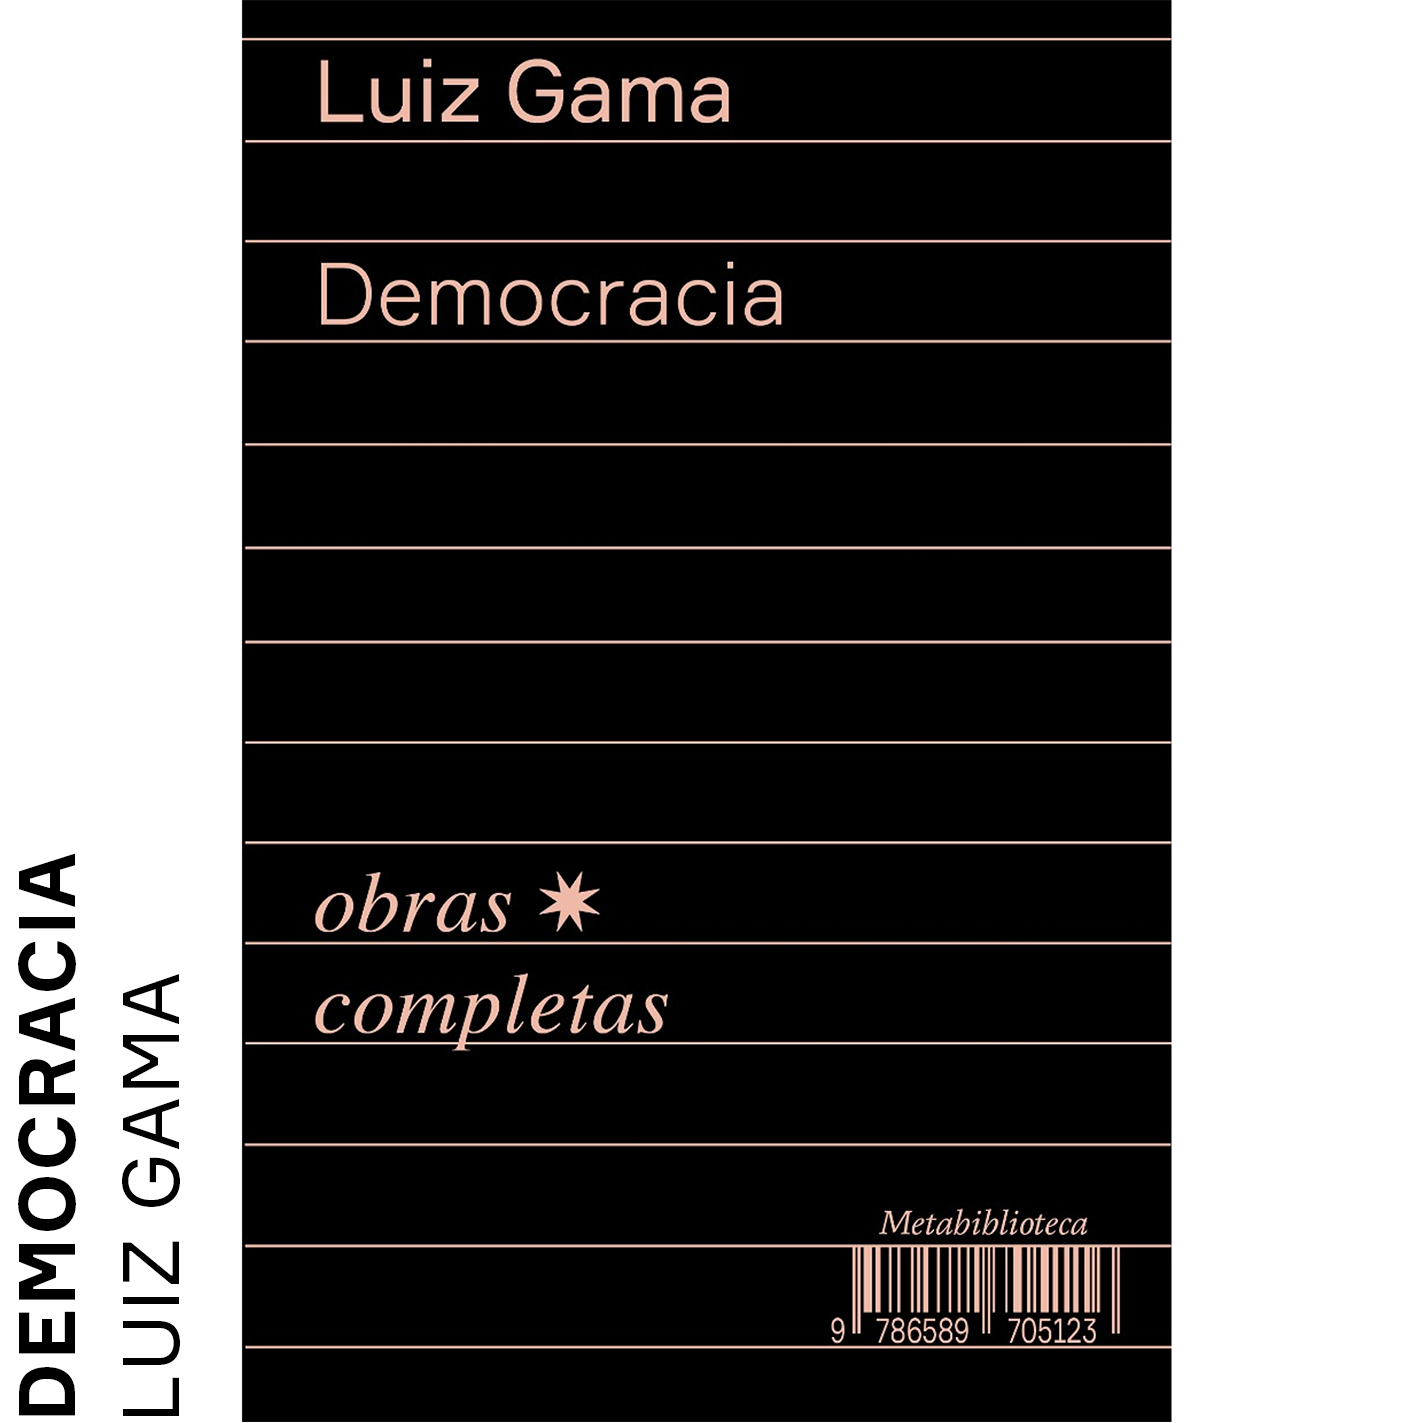
\includegraphics[width=40mm]{./GRID/HEDRA_DEMOCRACIA.png}}
\subfloat{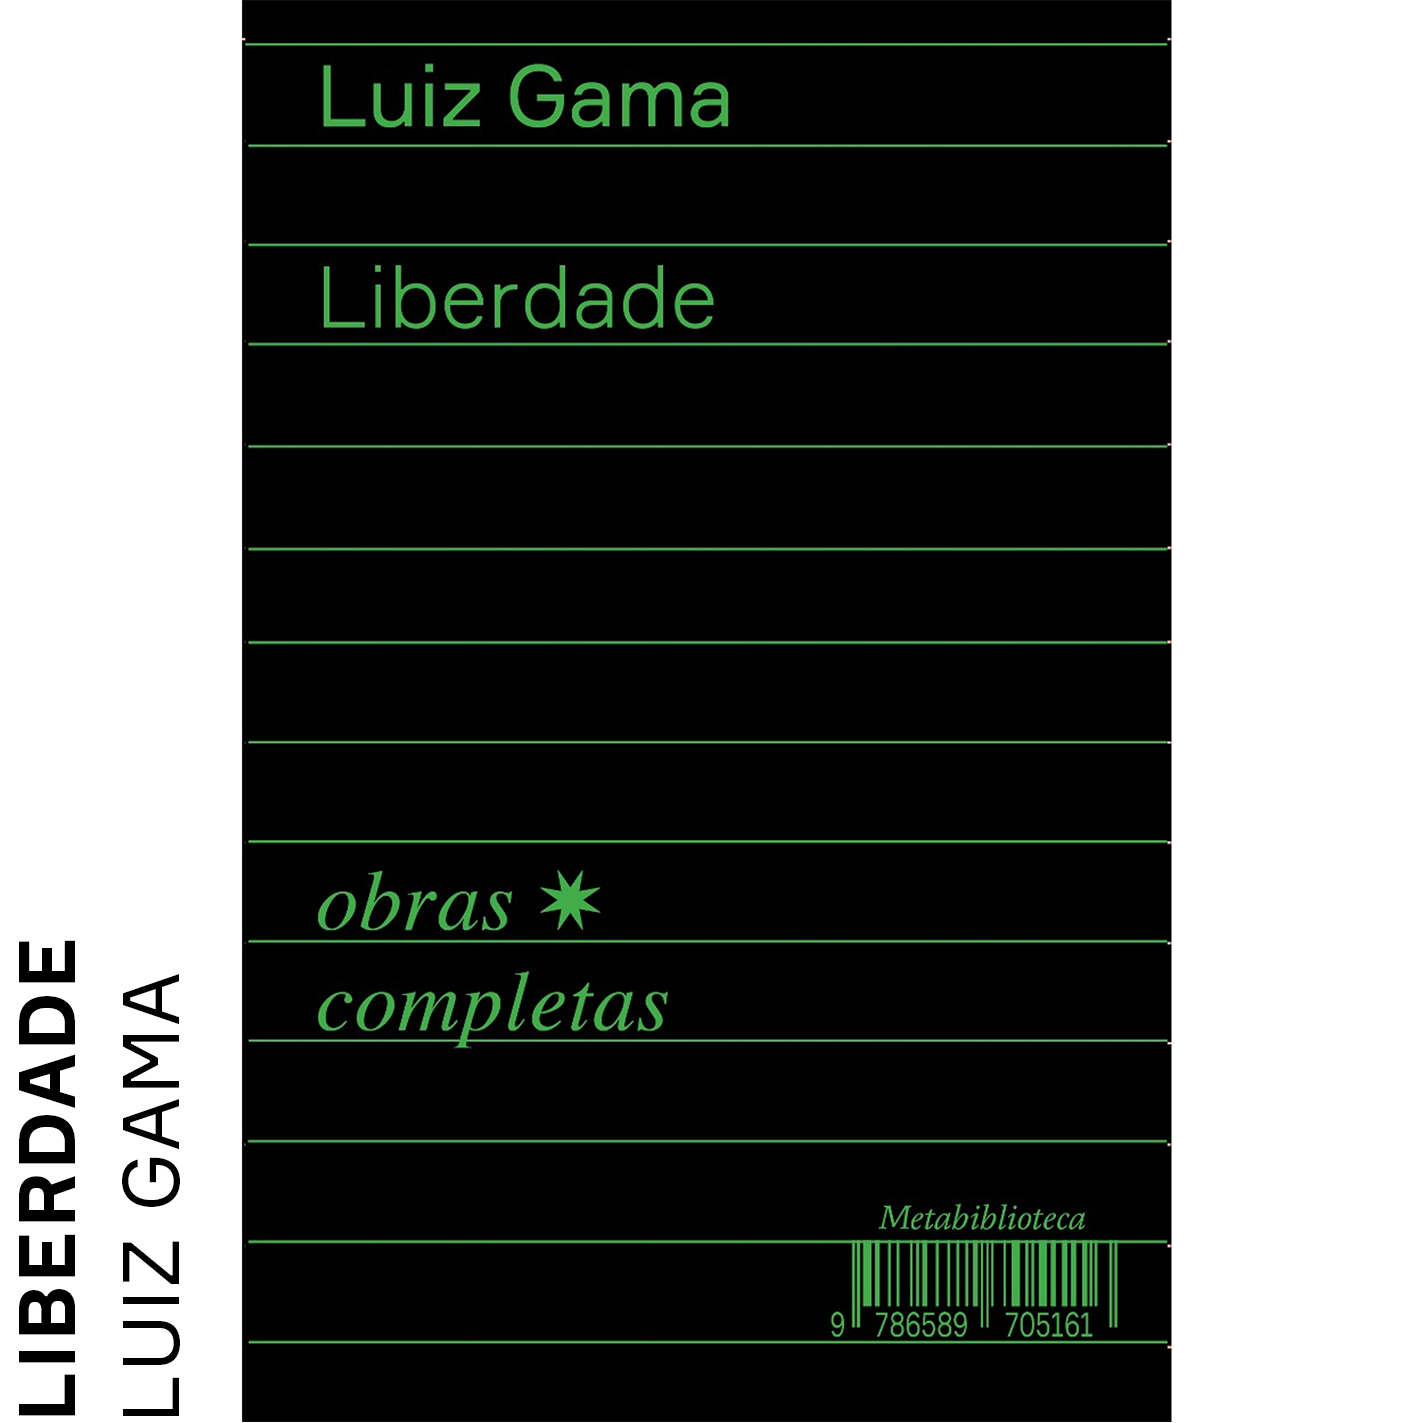
\includegraphics[width=40mm]{./GRID/HEDRA_LIBERDADE.png}}
\subfloat{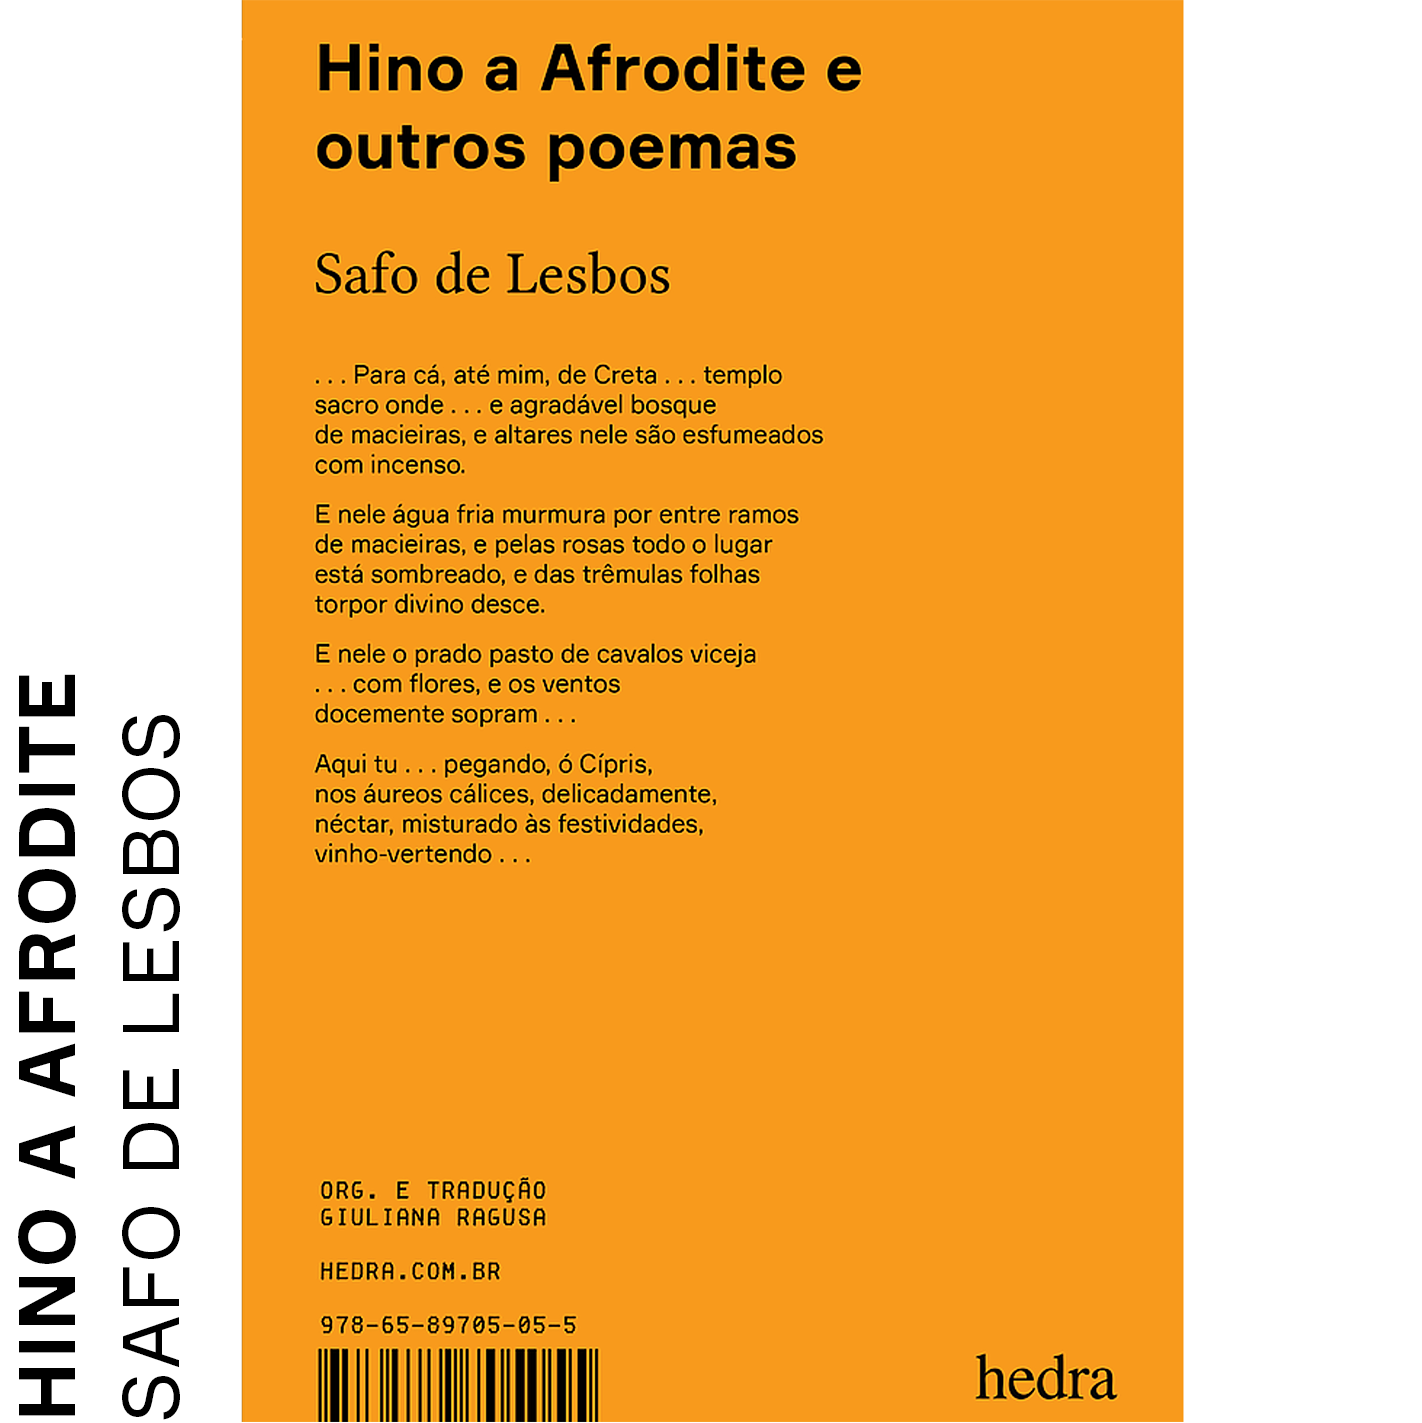
\includegraphics[width=40mm]{./GRID/HEDRA_SAFO.png}}\\\hspace*{.5cm}

\vspace{.5cm}

\subfloat{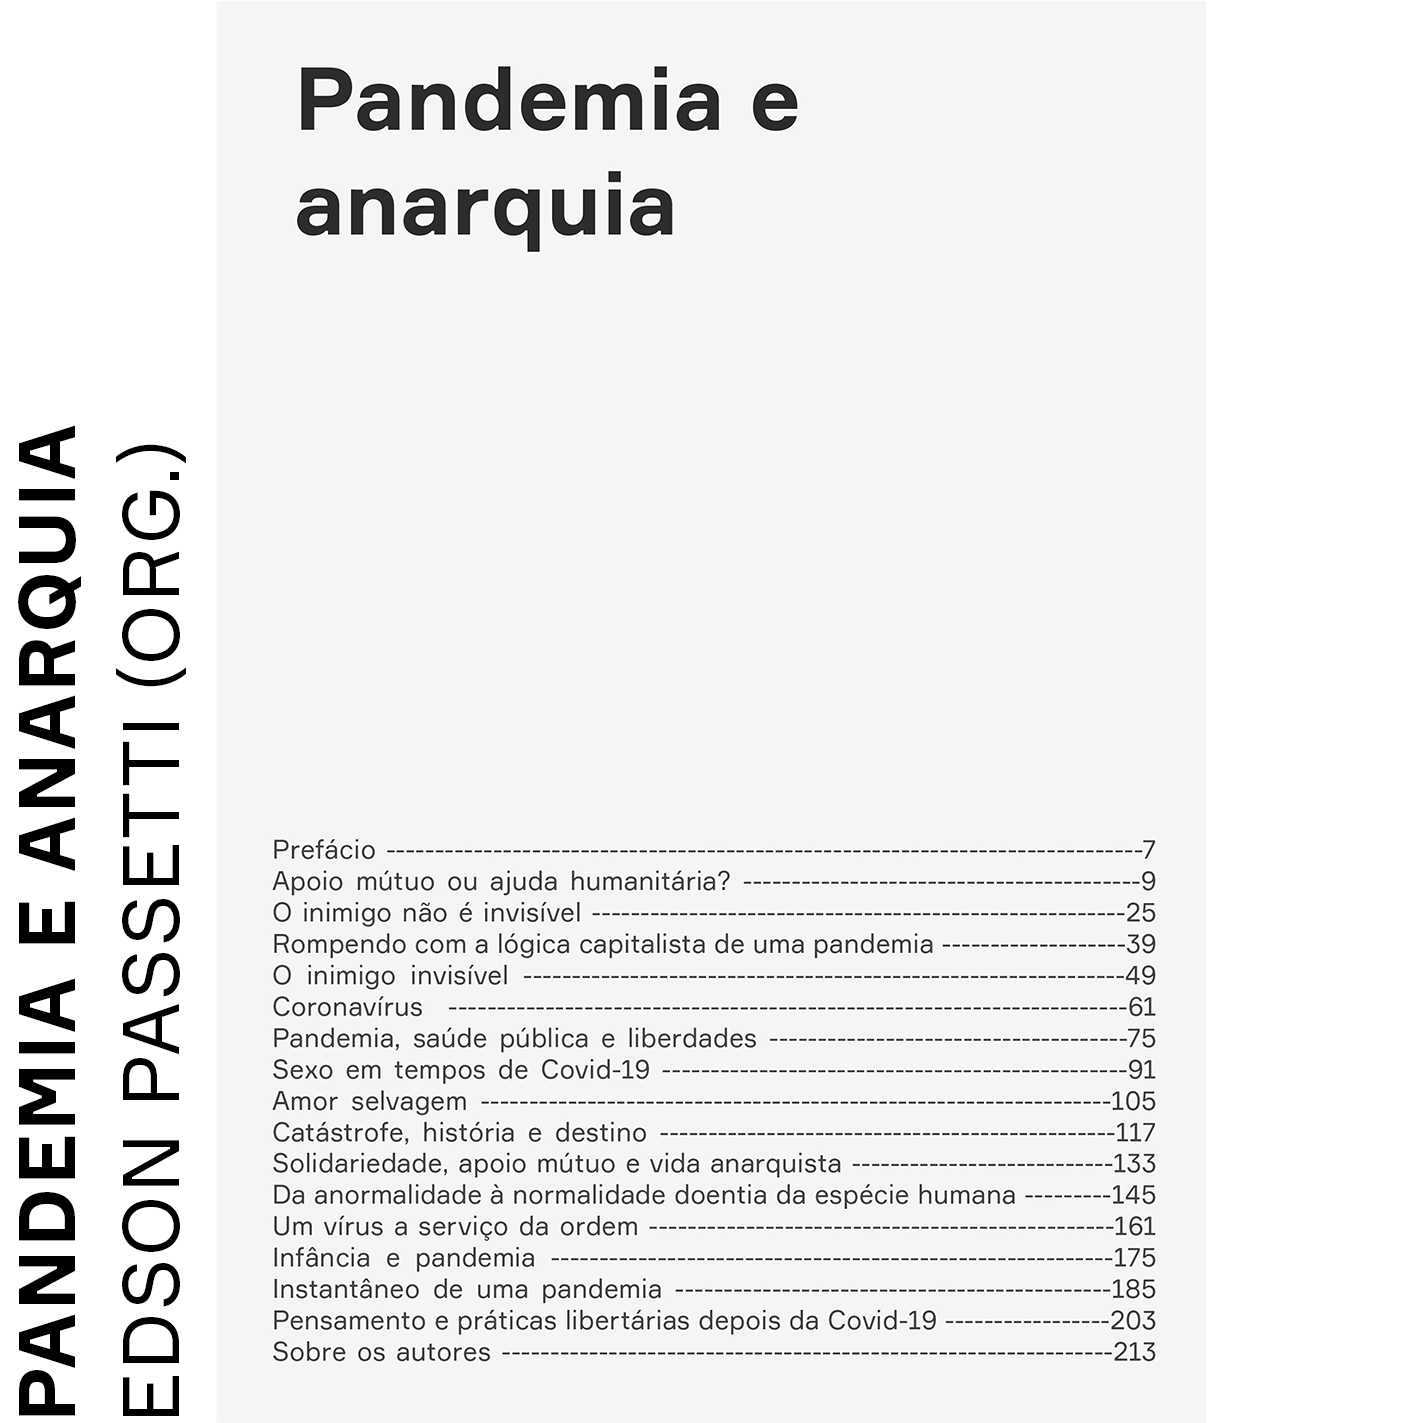
\includegraphics[width=40mm]{./GRID/HEDRA_PANDEMIA.png}}
\subfloat{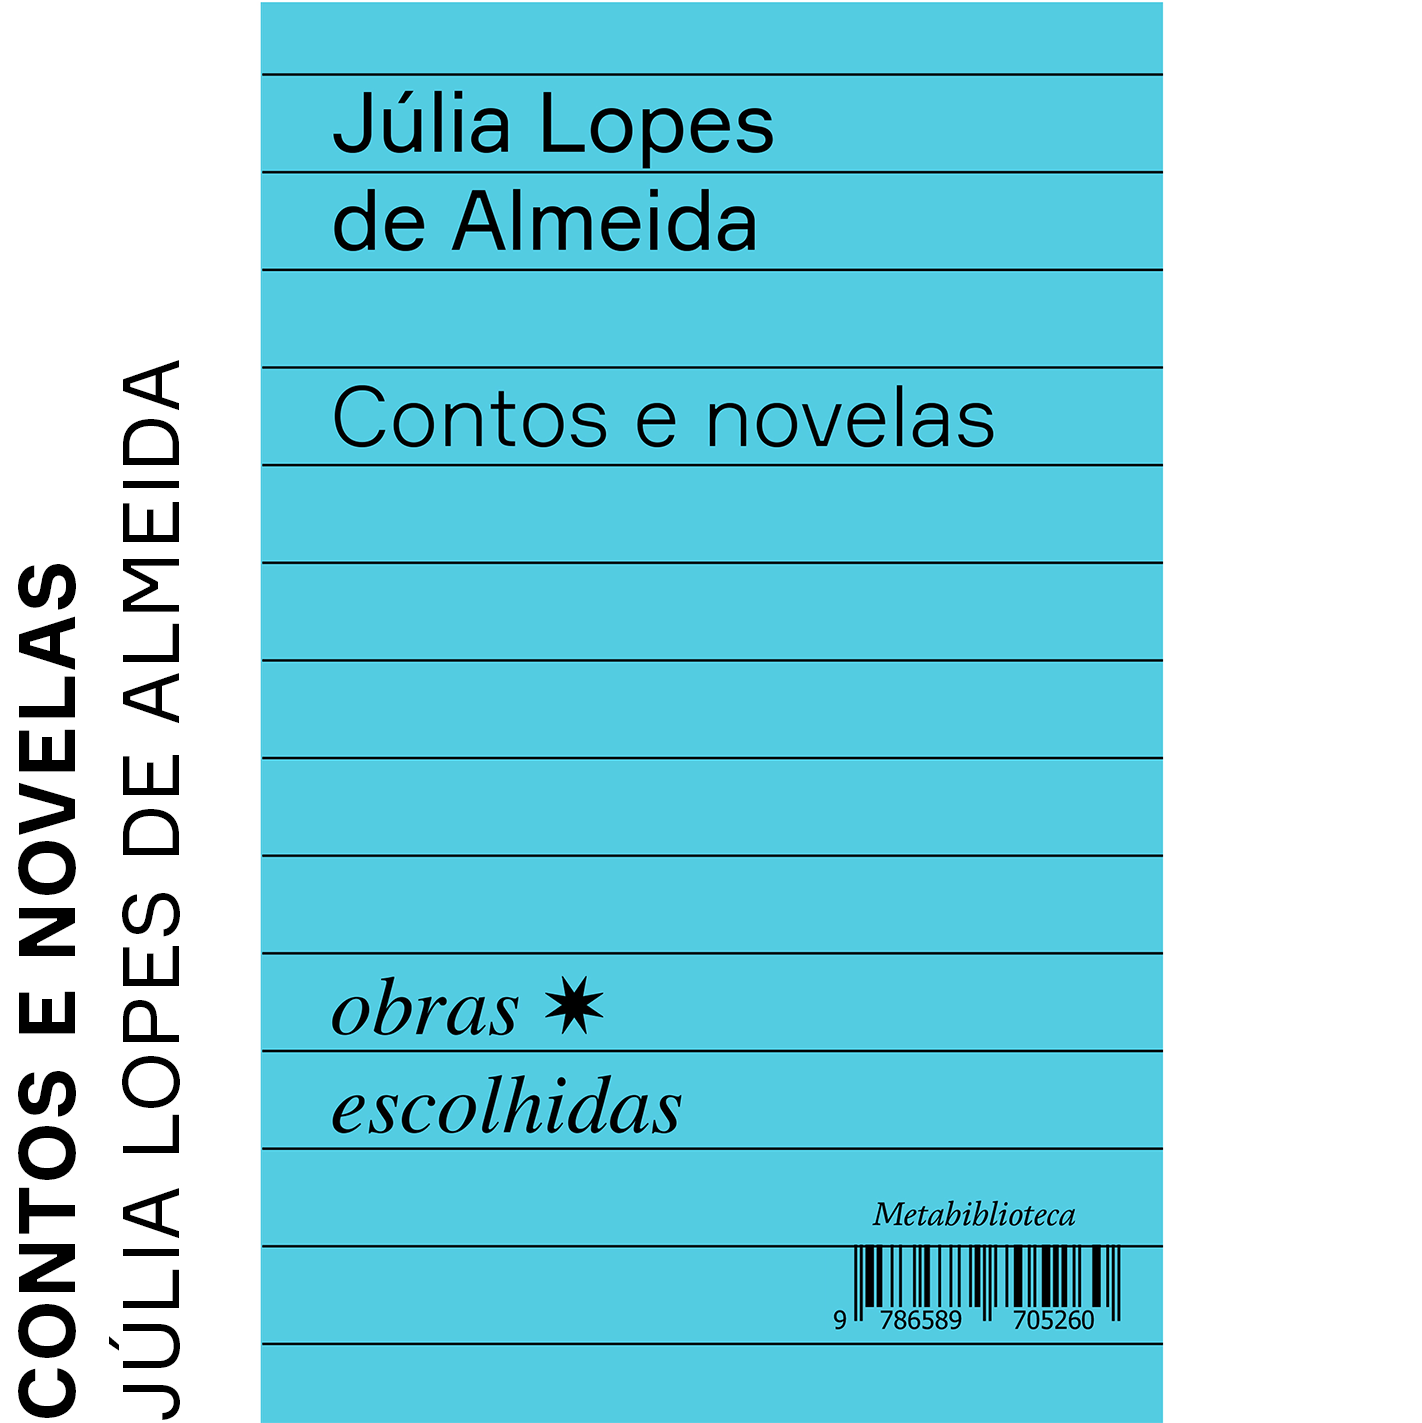
\includegraphics[width=40mm]{./GRID/HEDRA_JULIA.png}}
\subfloat{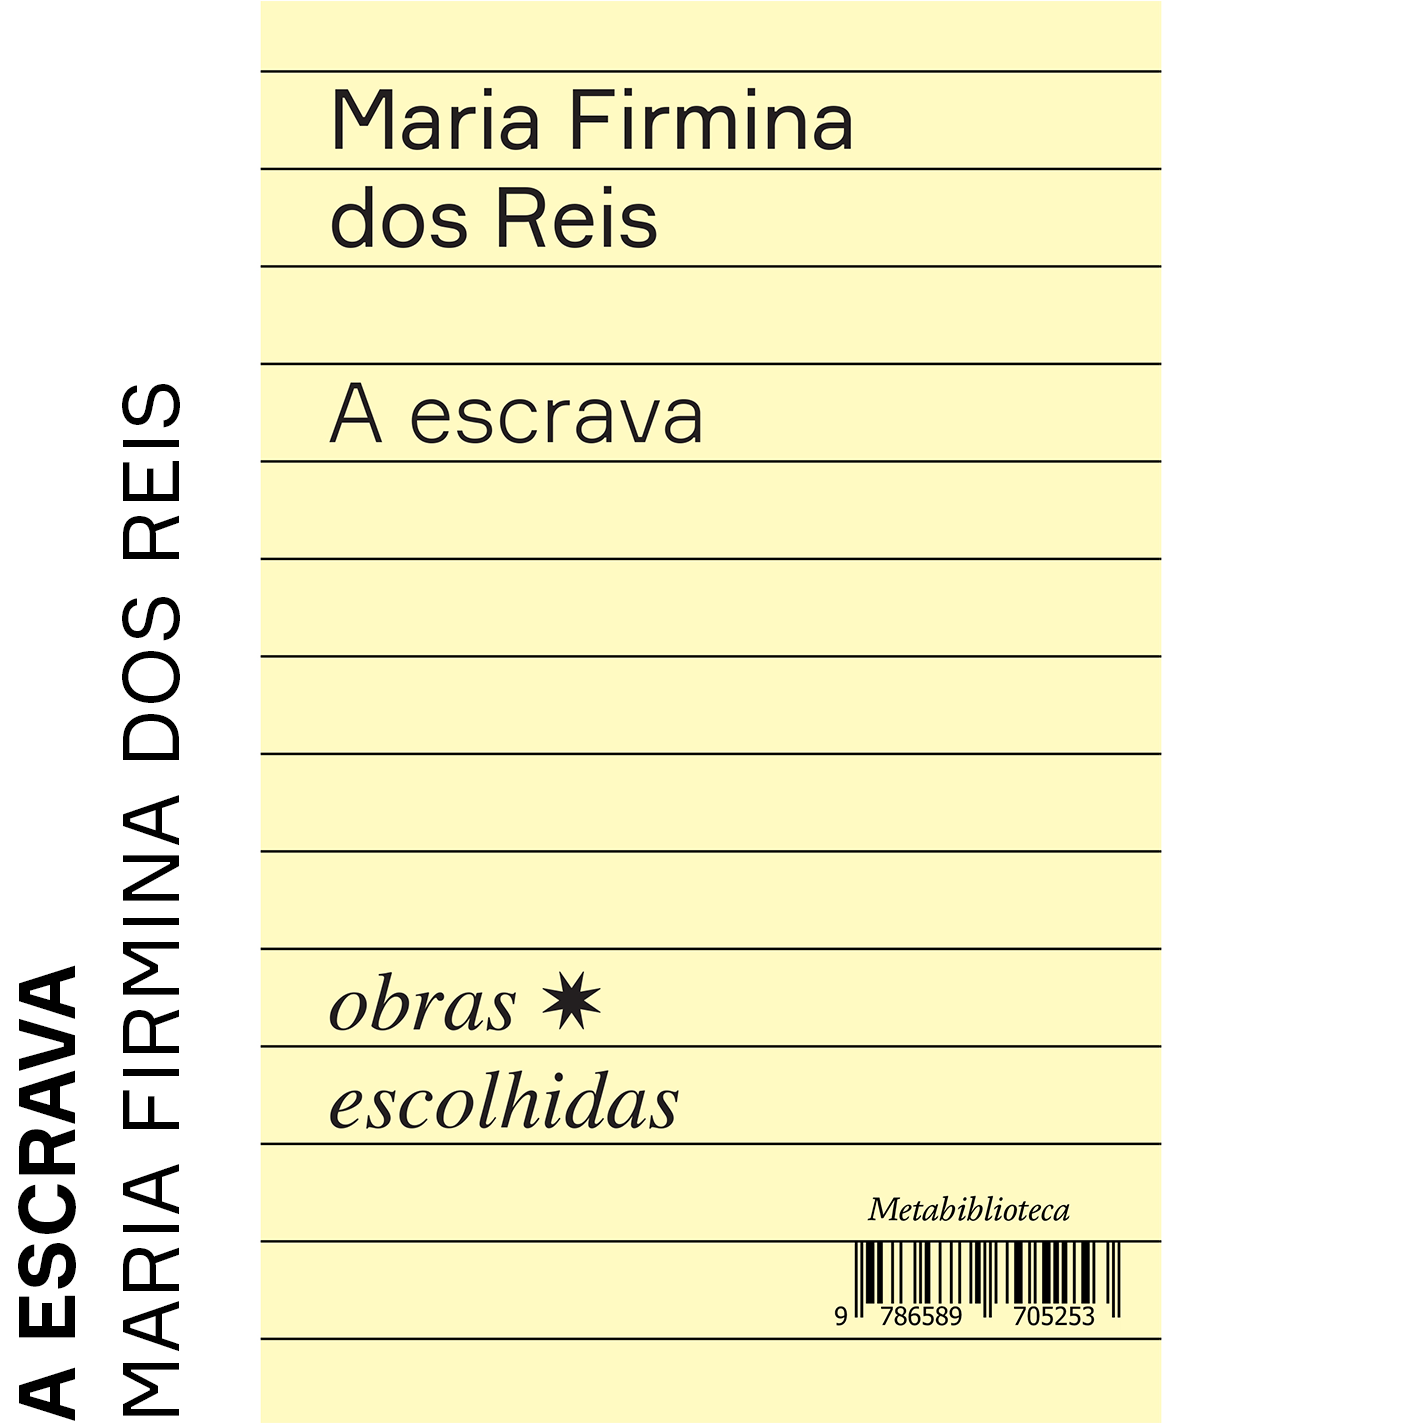
\includegraphics[width=40mm]{./GRID/HEDRA_FIRMINA.png}}\\\hspace*{.5cm}

\vspace{.5cm}

\subfloat{
\includegraphics[width=40mm]{./GRID/HEDRA_ARUAQUES.png}}
\subfloat{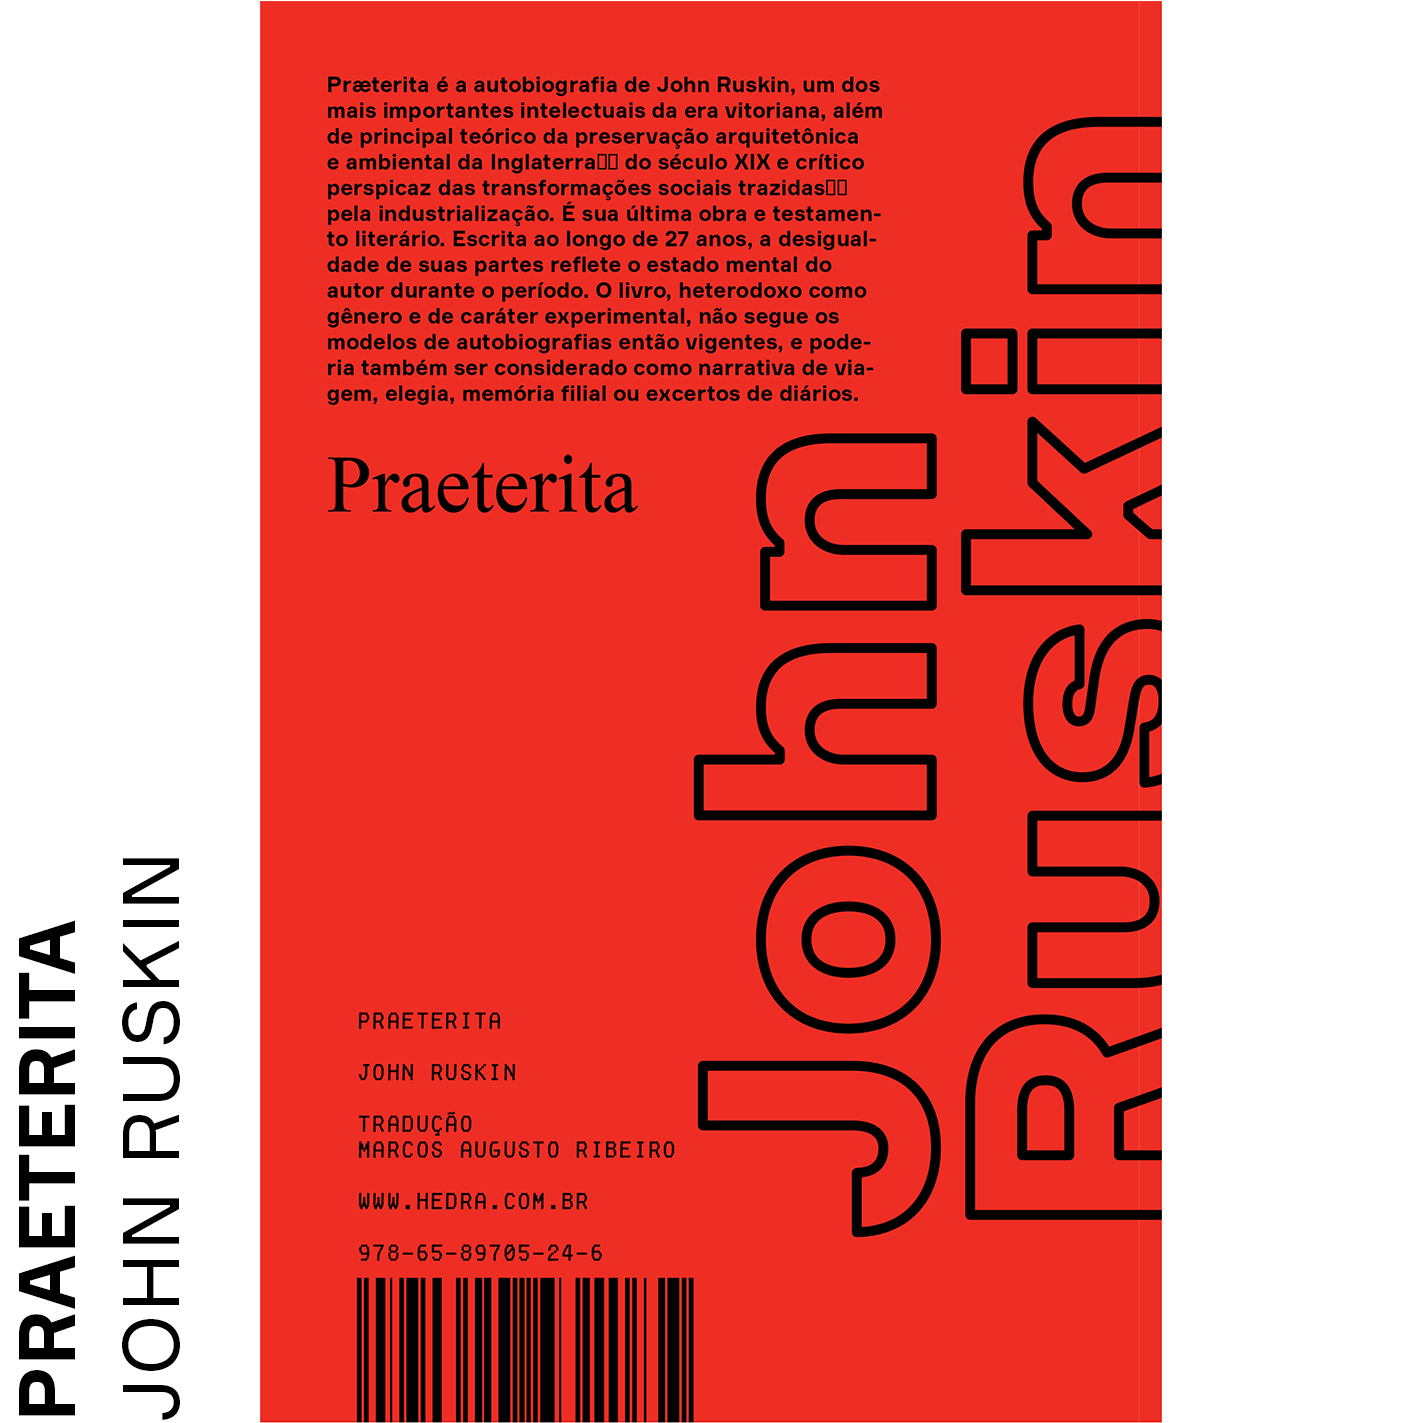
\includegraphics[width=40mm]{./GRID/HEDRA_RUSKIN.png}}
\subfloat{
\includegraphics[width=40mm]{./GRID/HEDRA_SOCIEDADE.png}}\\\hspace*{.5cm}

\vspace{.5cm}

\subfloat{
\includegraphics[width=40mm]{./GRID/HEDRA_ATIVISMO.png}}
\subfloat{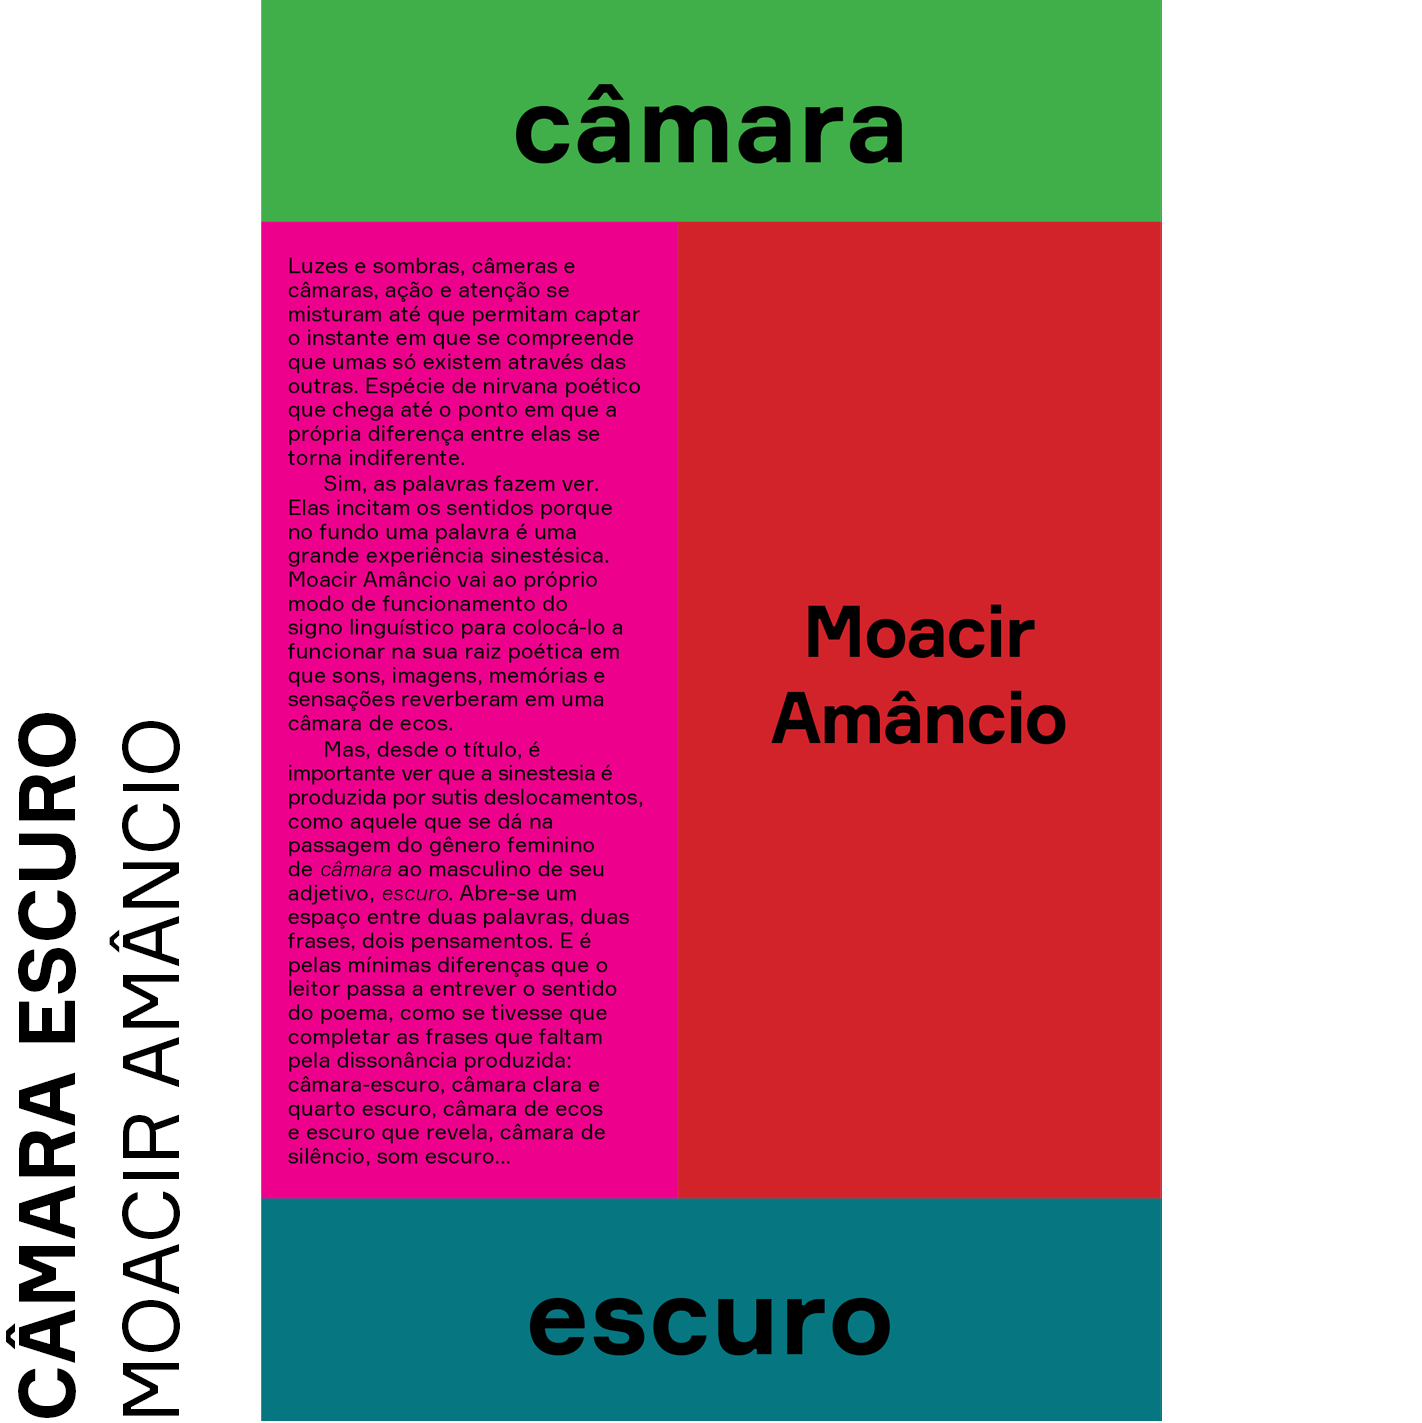
\includegraphics[width=40mm]{./GRID/HEDRA_CAMARA.png}}
\subfloat{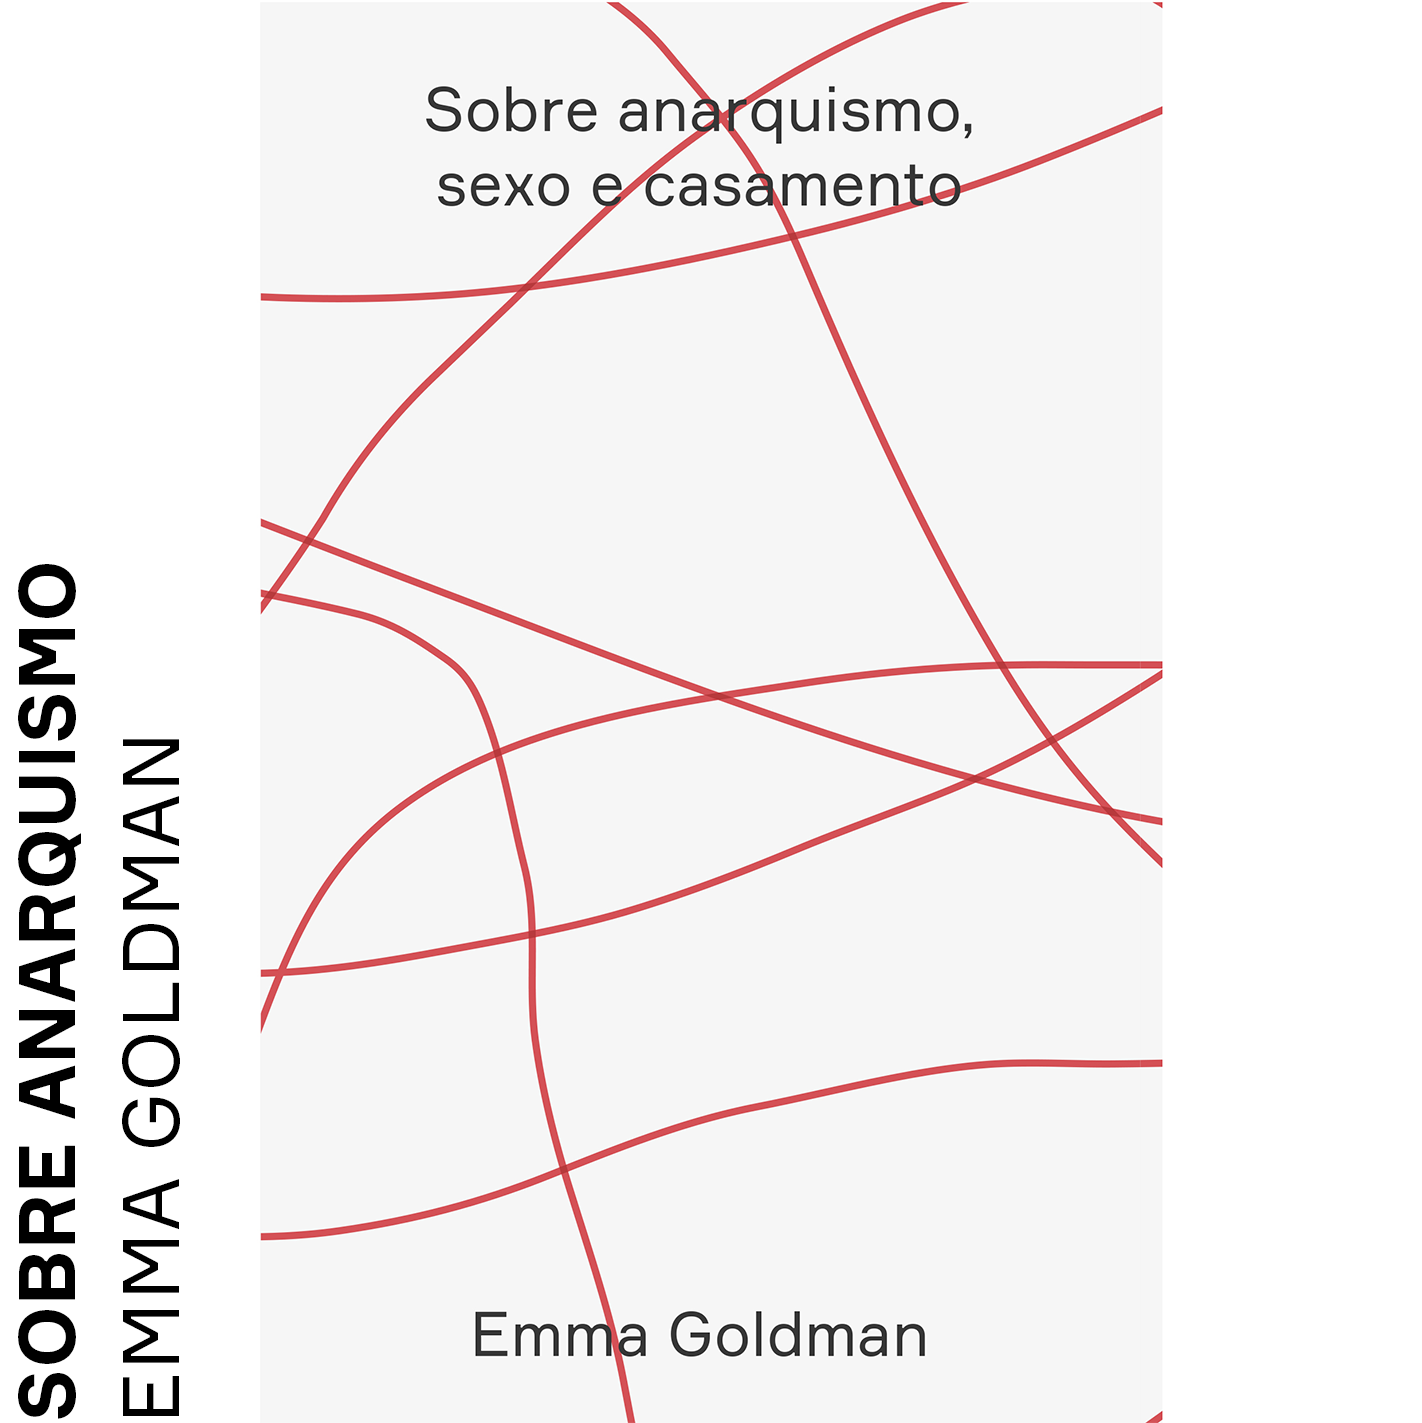
\includegraphics[width=40mm]{./GRID/HEDRA_GOLDMAN.png}}\\\hspace*{.5cm}
\end{tabular}
\end{figure}
\pagebreak

\pagestyle{grid}
\begin{figure}[!htbp]
\begin{tabular}{cccc}
\vspace{.5cm}
\hspace*{.5cm}
\subfloat{
\includegraphics[width=40mm]{./GRID/HEDRA_DESINFORMACAO.png}}
\subfloat{
\includegraphics[width=40mm]{./GRID/HEDRA_ROBINSON.png}}
\subfloat{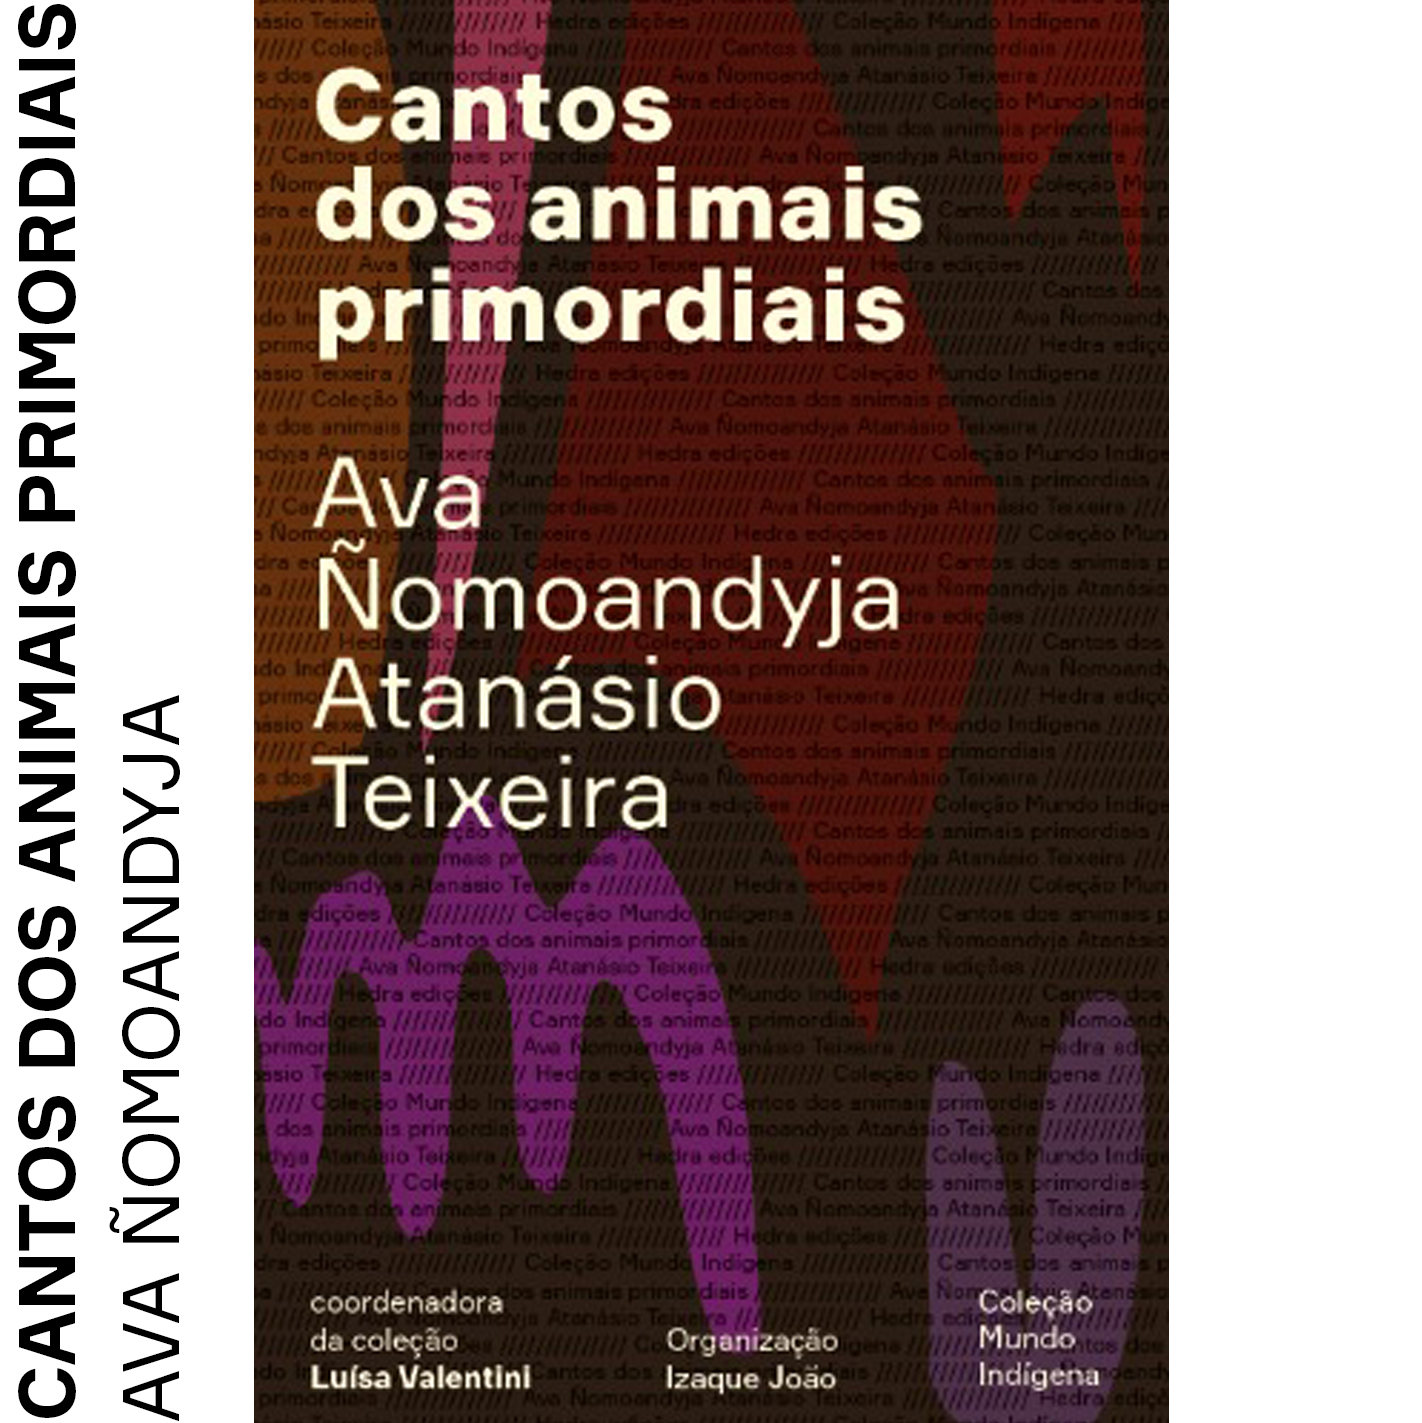
\includegraphics[width=40mm]{./GRID/HEDRA_CANTOS.png}}\\\hspace*{.5cm}

\vspace{.5cm}

\subfloat{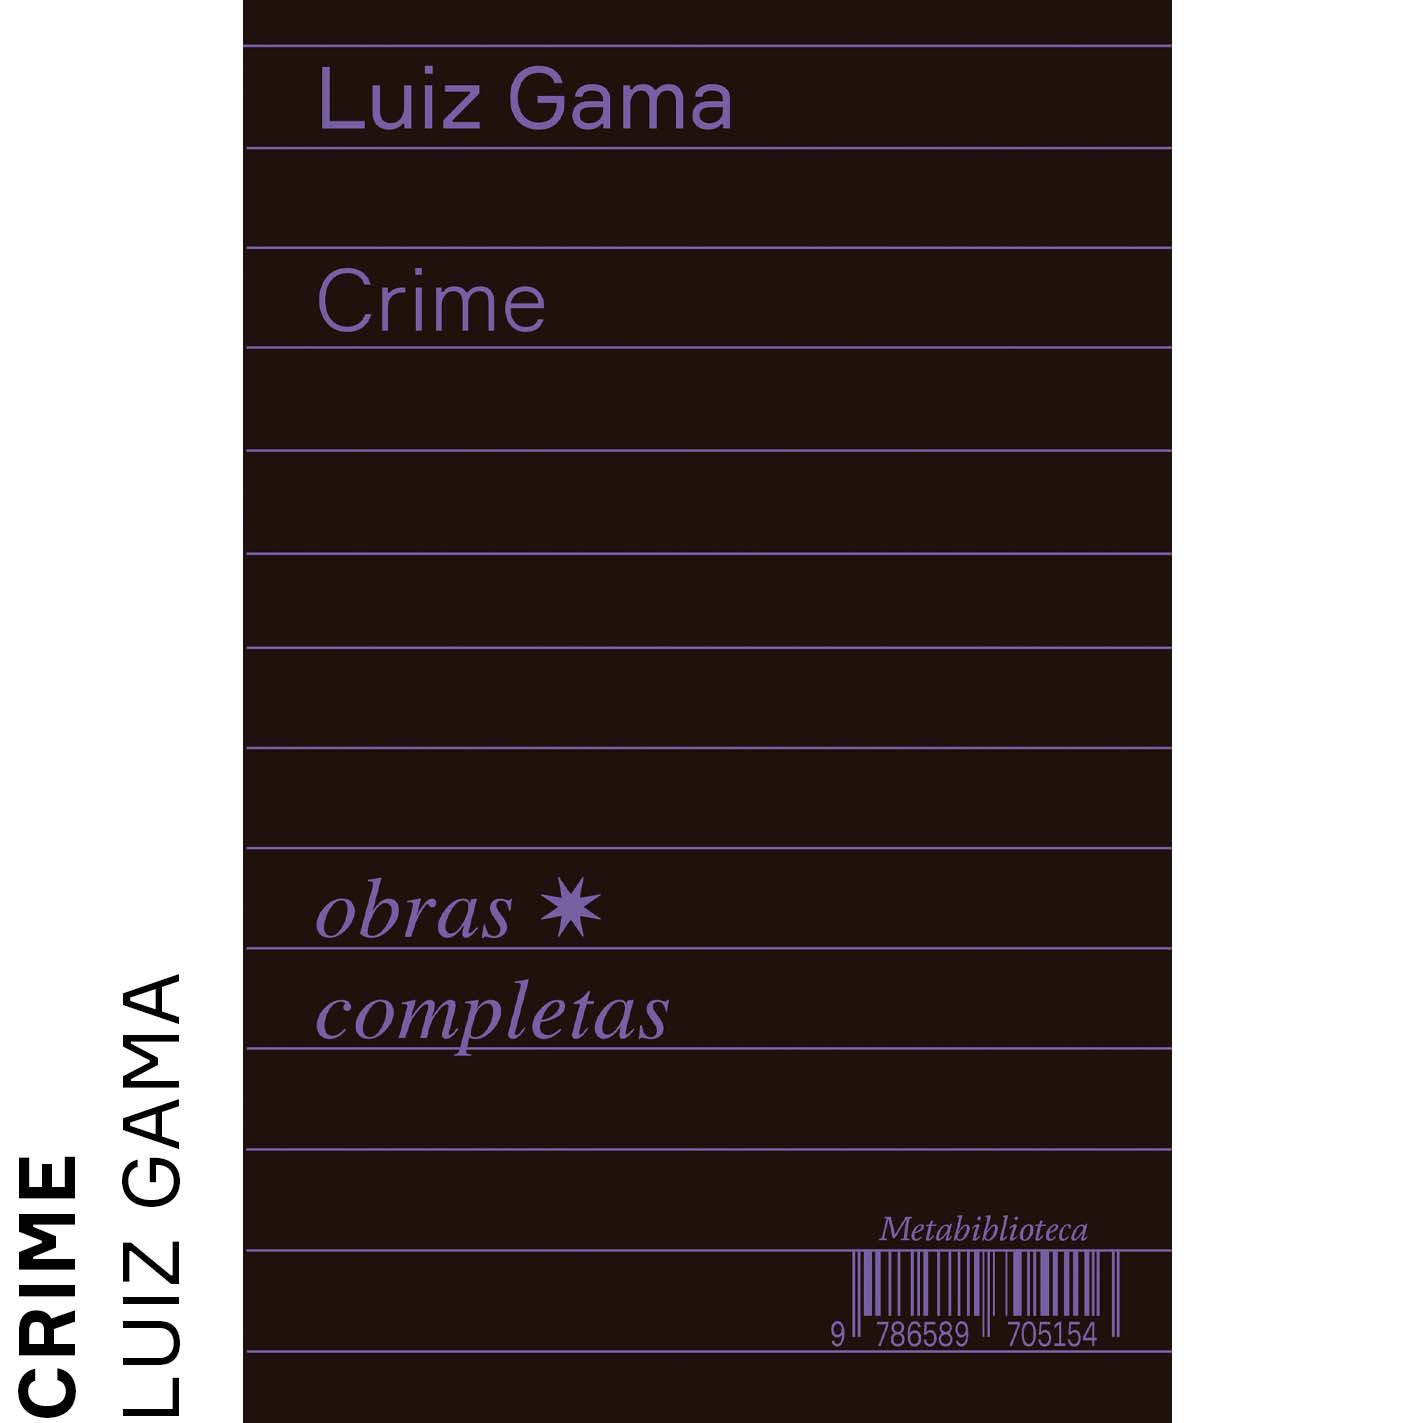
\includegraphics[width=40mm]{./GRID/HEDRA_CRIME.png}}
\subfloat{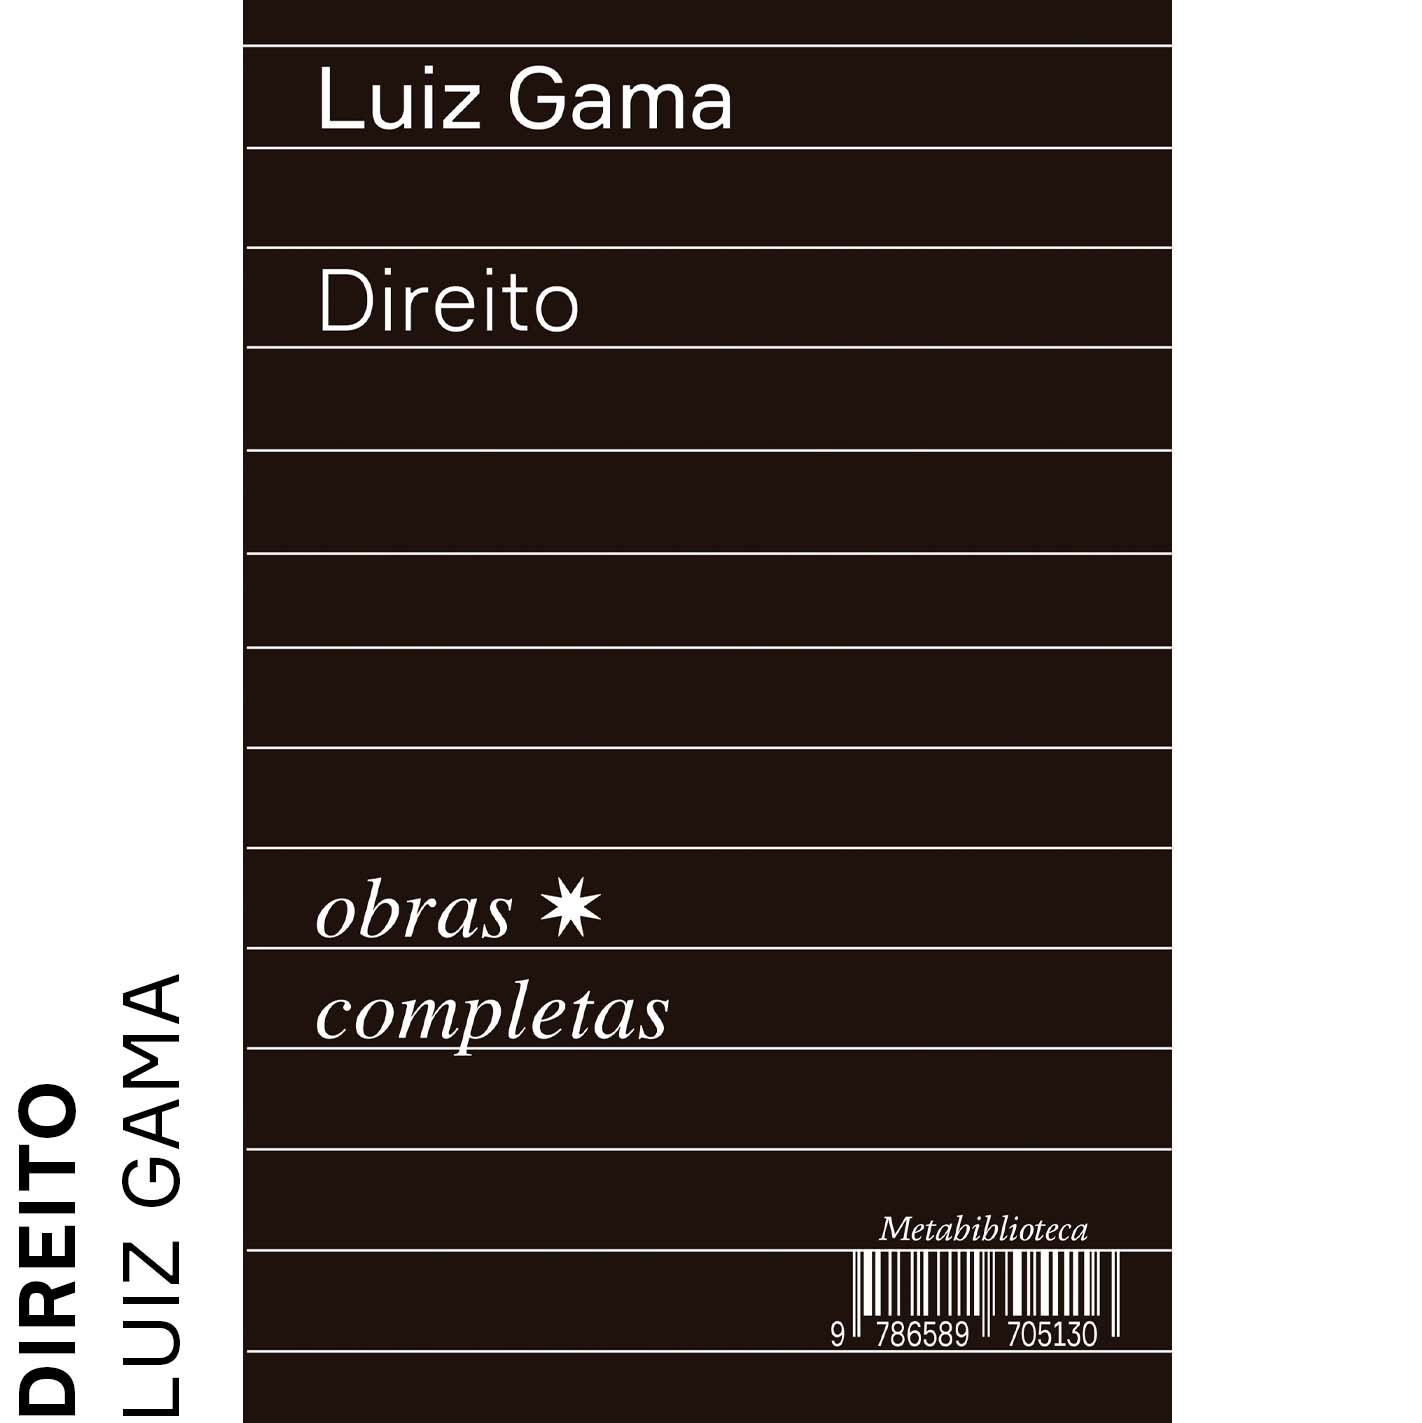
\includegraphics[width=40mm]{./GRID/HEDRA_DIREITO.png}}
\subfloat{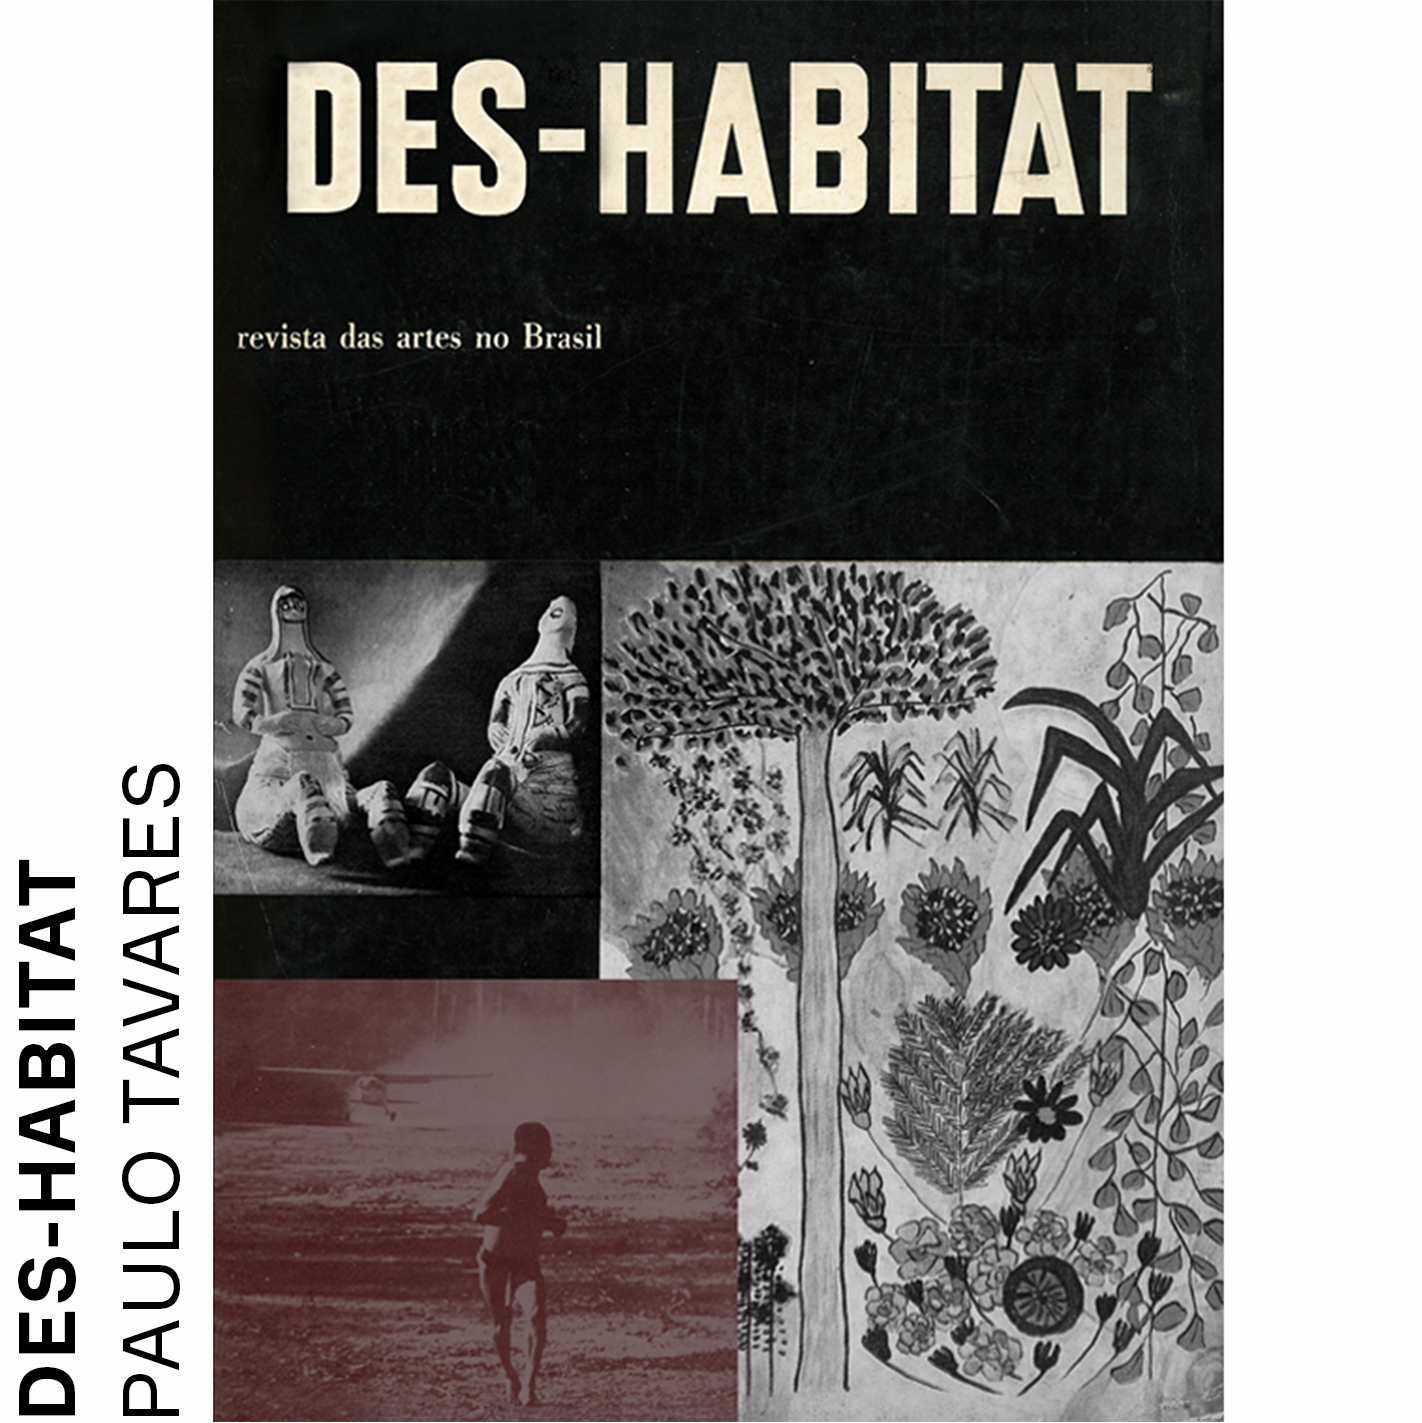
\includegraphics[width=40mm]{./GRID/N-1_HABITAT.png}}\\\hspace*{.5cm}

\vspace{.5cm}

\subfloat{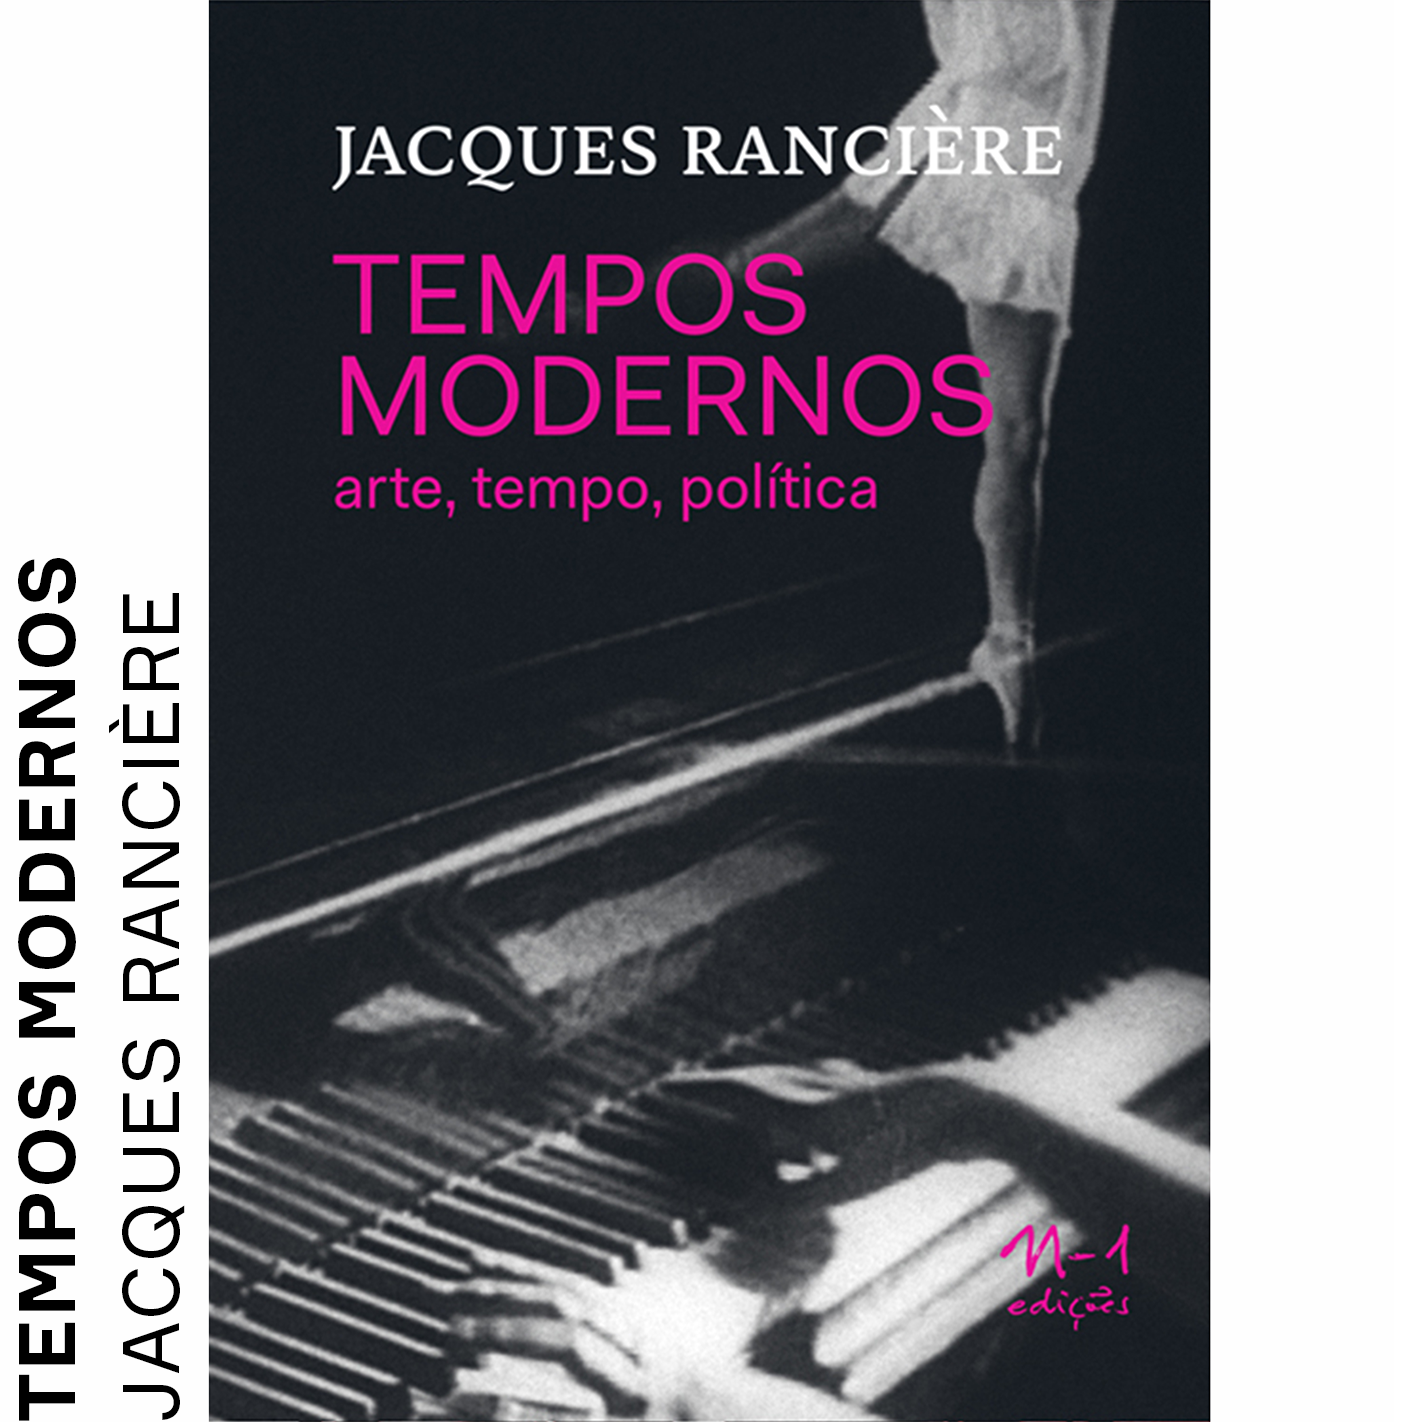
\includegraphics[width=40mm]{./GRID/N-1_JACQUES.png}}
\subfloat{
\includegraphics[width=40mm]{./GRID/N-1_POVO.png}}
\subfloat{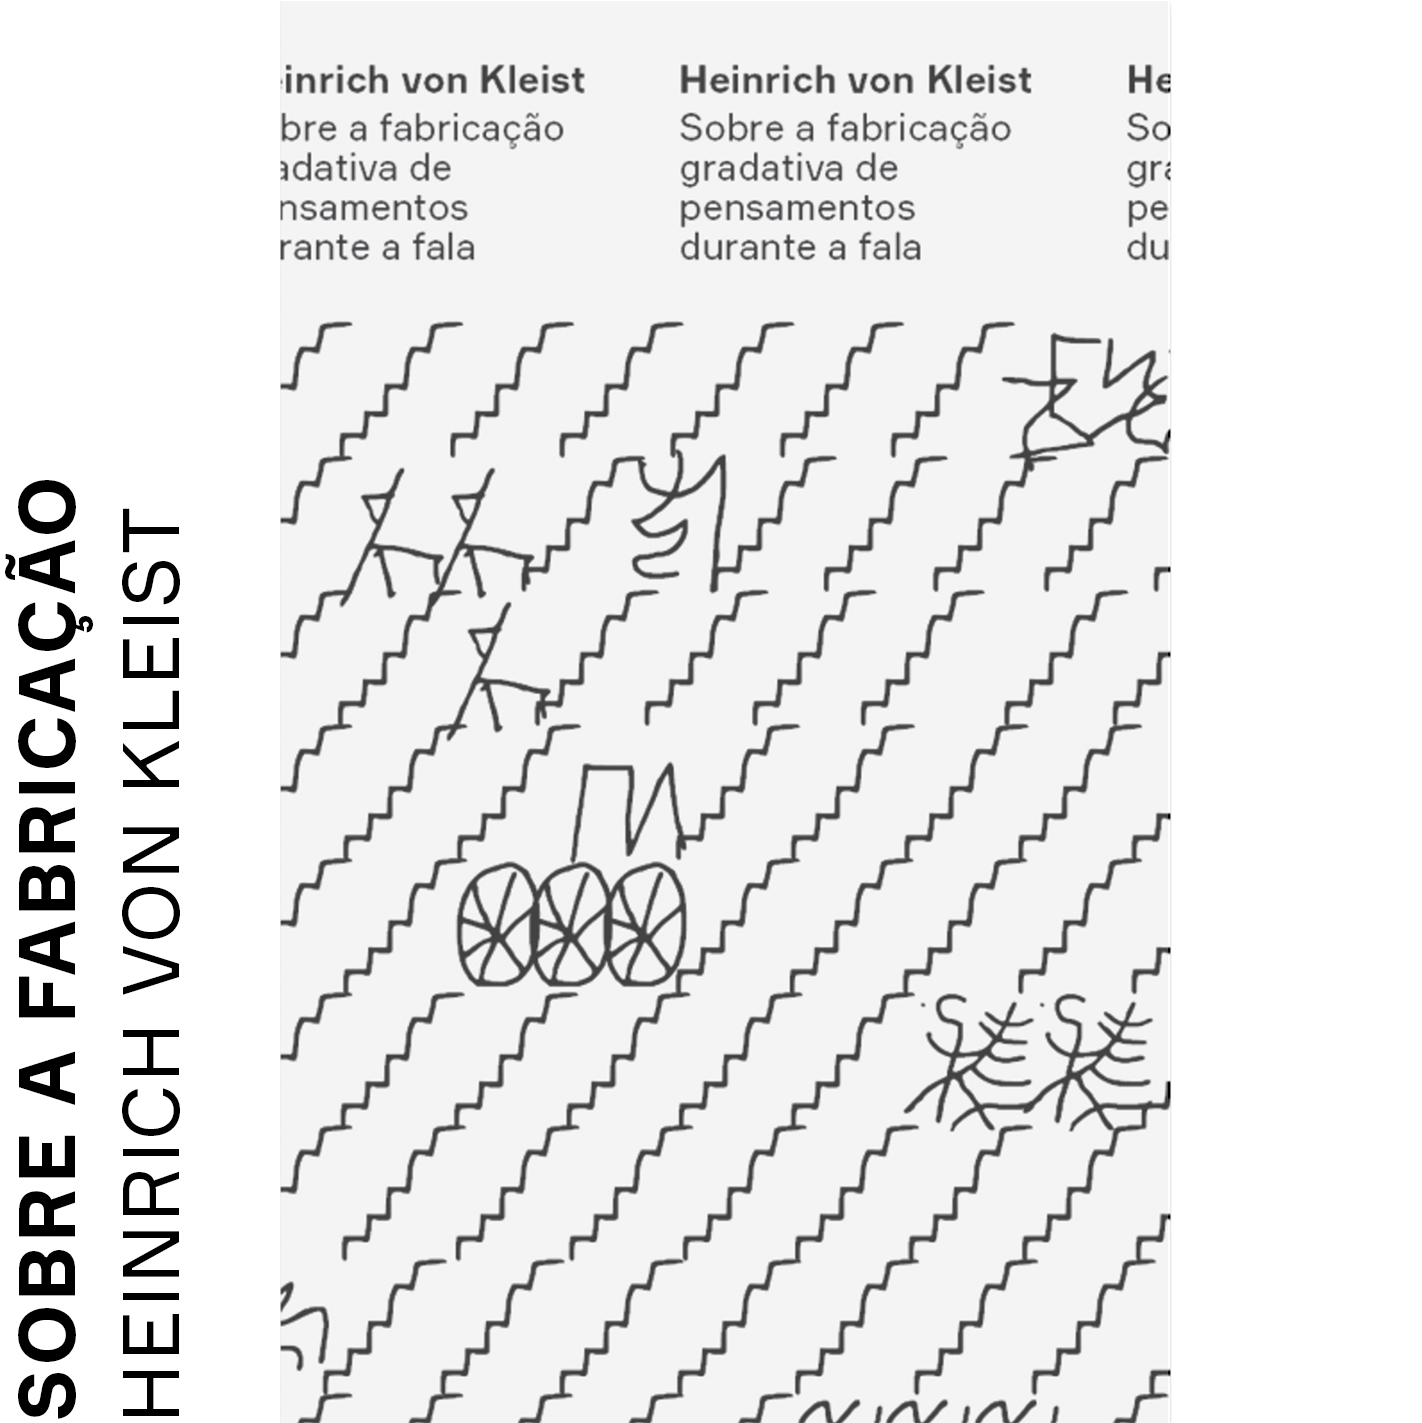
\includegraphics[width=40mm]{./GRID/N-1_FABRICACAO.png}}\\\hspace*{.5cm}

\vspace{.5cm}

\subfloat{
\includegraphics[width=40mm]{./GRID/N-1_EXPERIENCIA.png}}
\subfloat{
\includegraphics[width=40mm]{./GRID/N-1_HIDRA.png}}
\subfloat{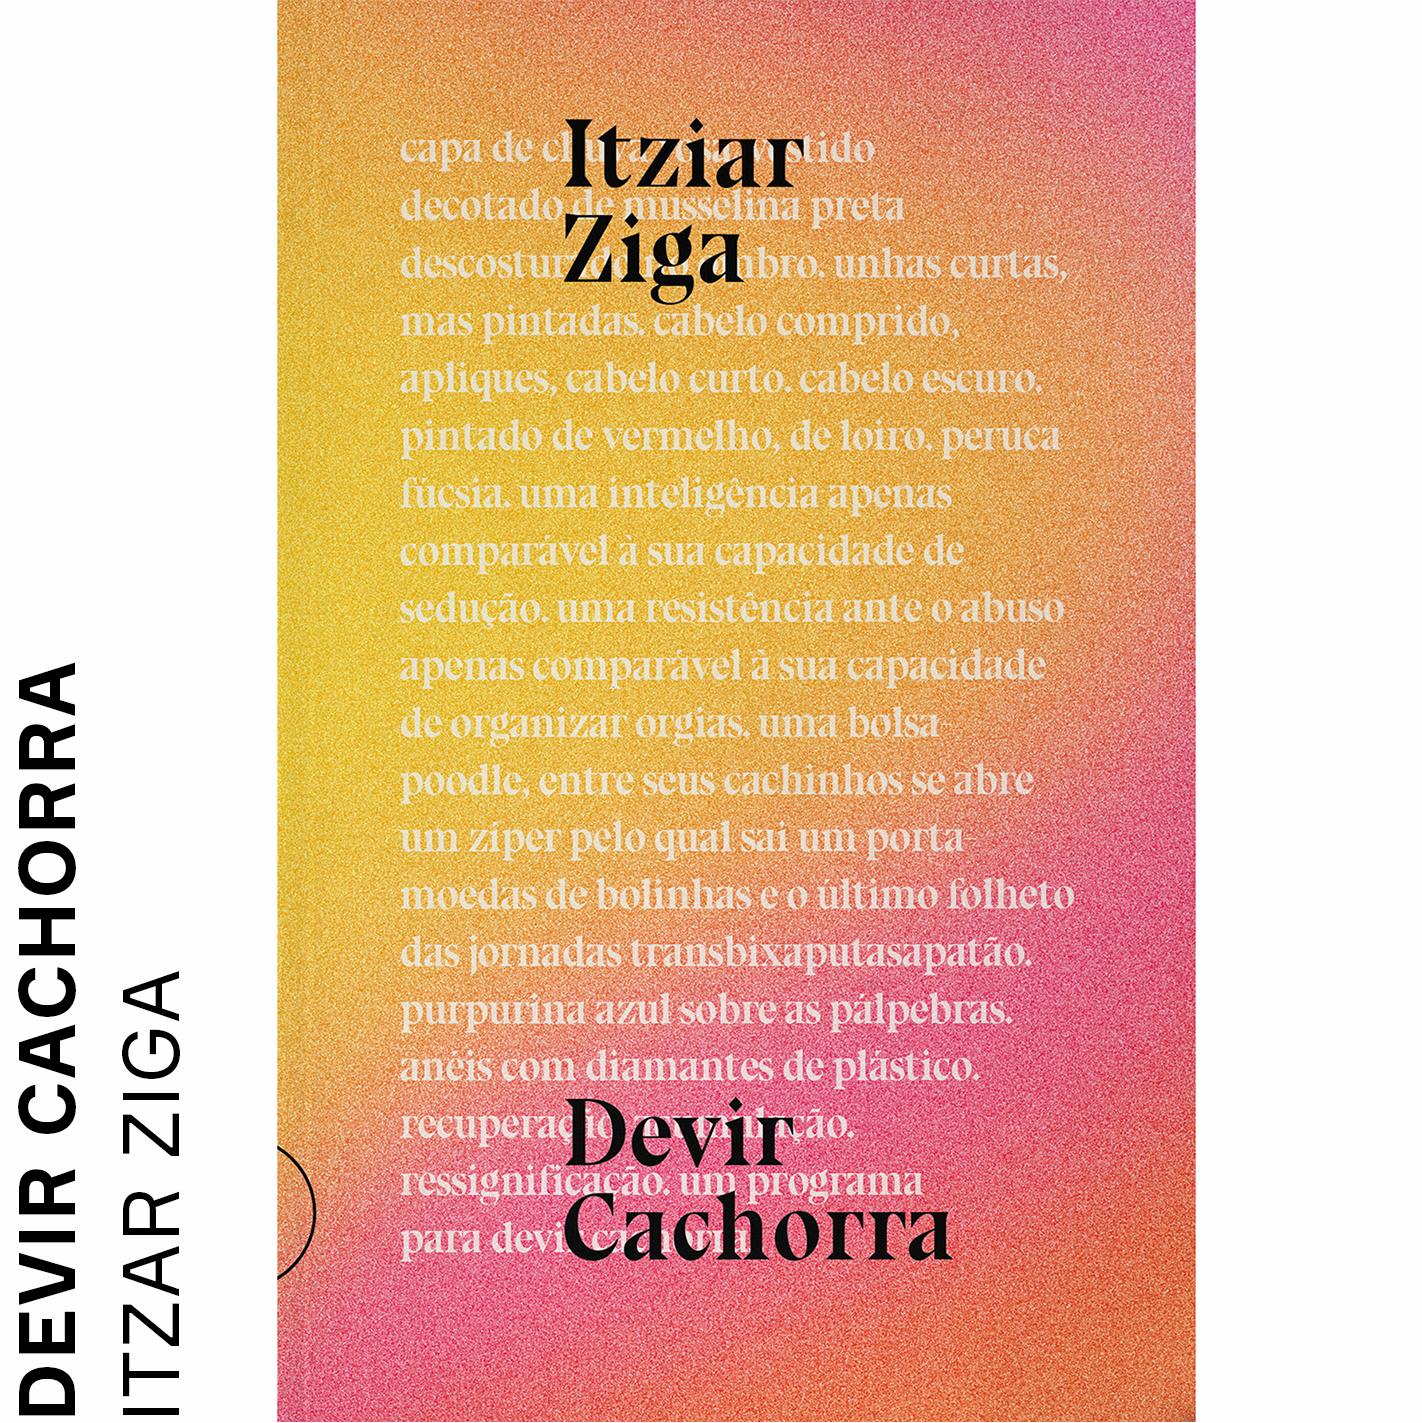
\includegraphics[width=40mm]{./GRID/N-1_DEVIR.png}}\\\hspace*{.5cm}
\end{tabular}
\end{figure}
\pagebreak

\pagestyle{grid}
\begin{figure}[!htbp]
\begin{tabular}{cccc}
\vspace{.5cm}
\hspace*{.5cm}
\subfloat{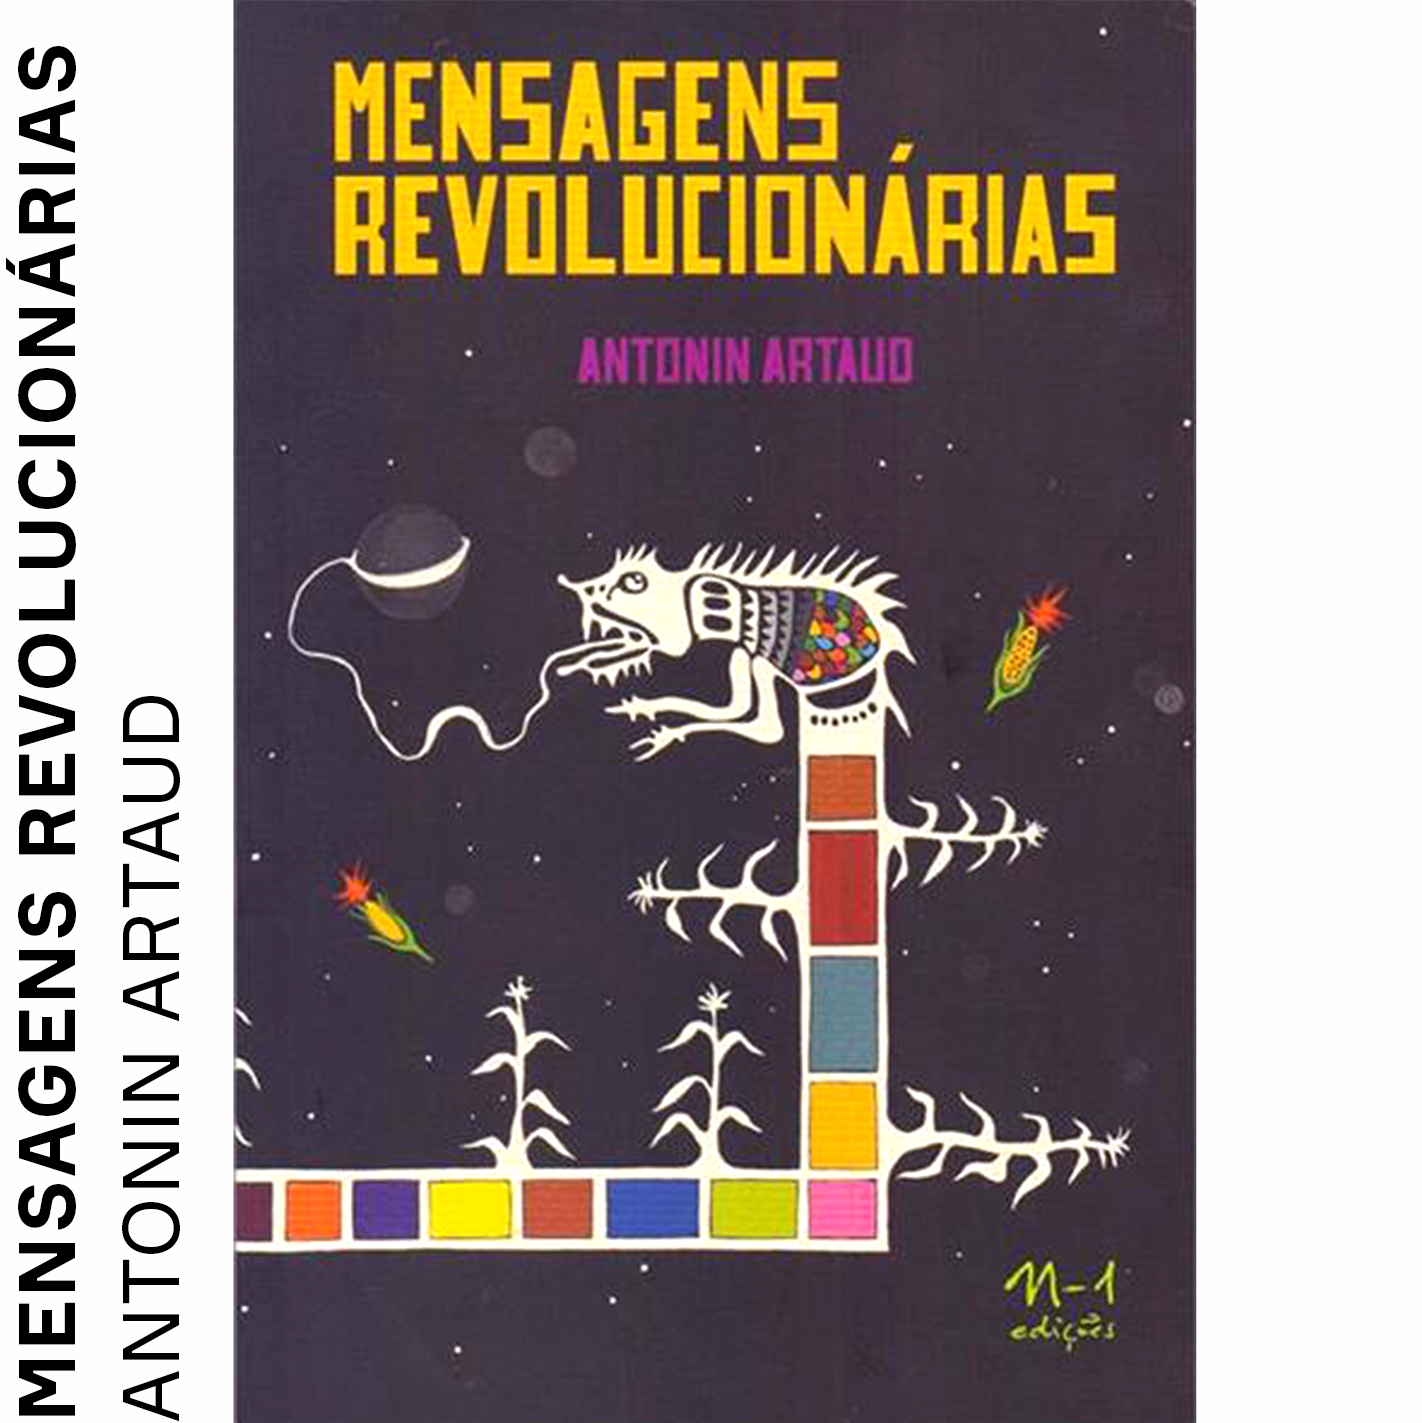
\includegraphics[width=40mm]{./GRID/N-1_MENSAGENS.png}}
\subfloat{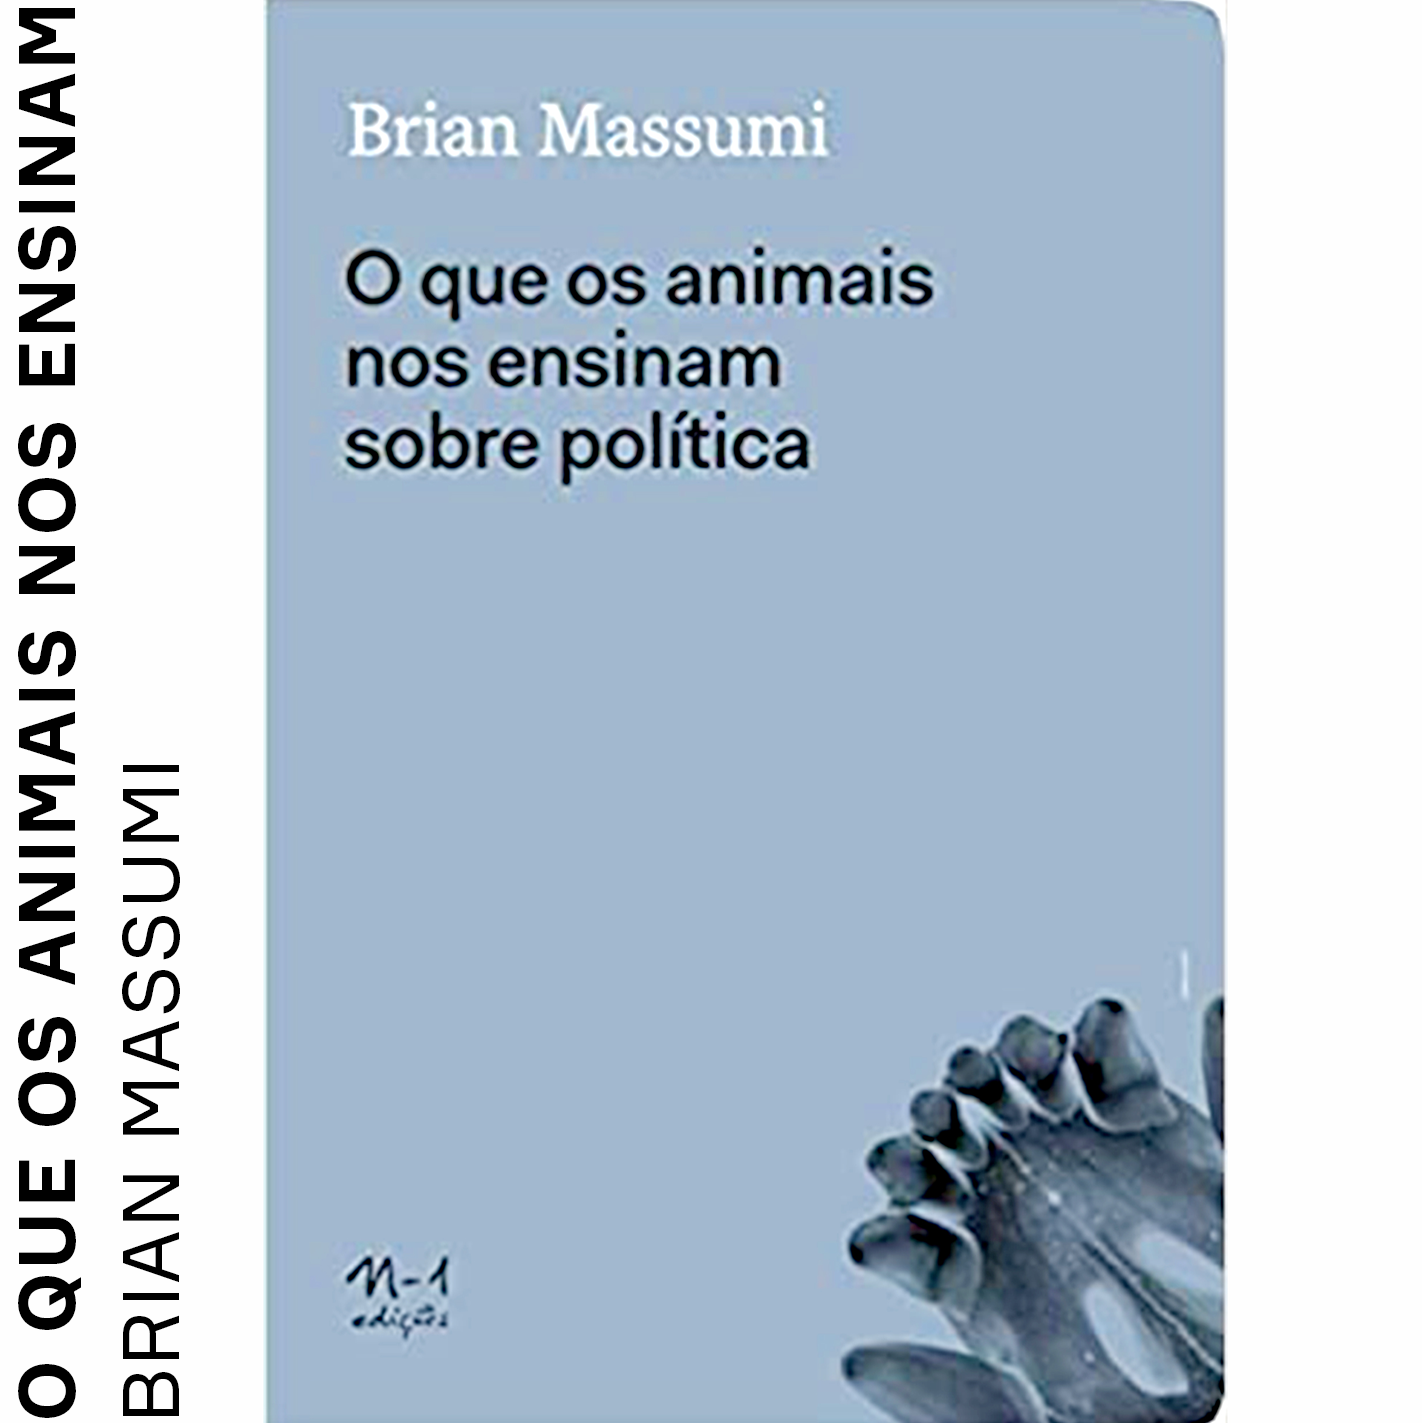
\includegraphics[width=40mm]{./GRID/N-1_ANIMAIS.png}}
\subfloat{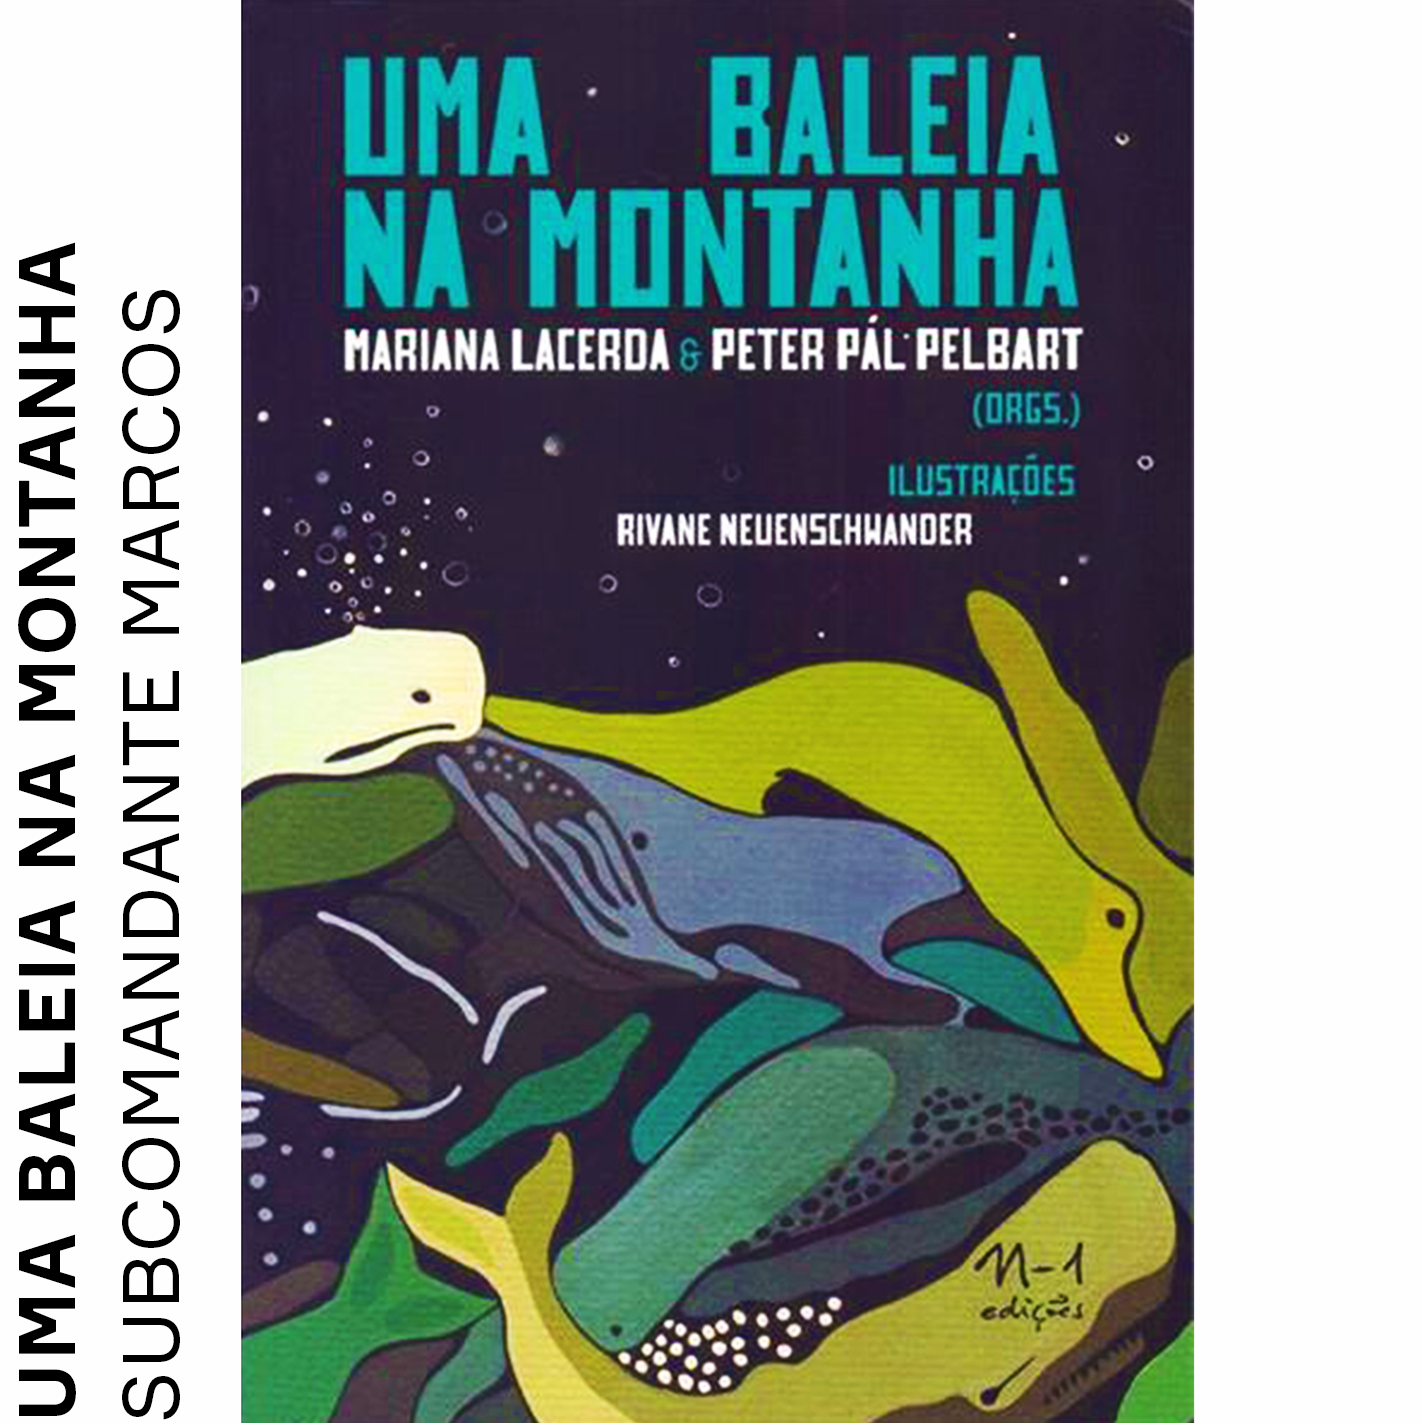
\includegraphics[width=40mm]{./GRID/N-1_BALEIA.png}}\\\hspace*{.5cm}

\vspace{.5cm}

\subfloat{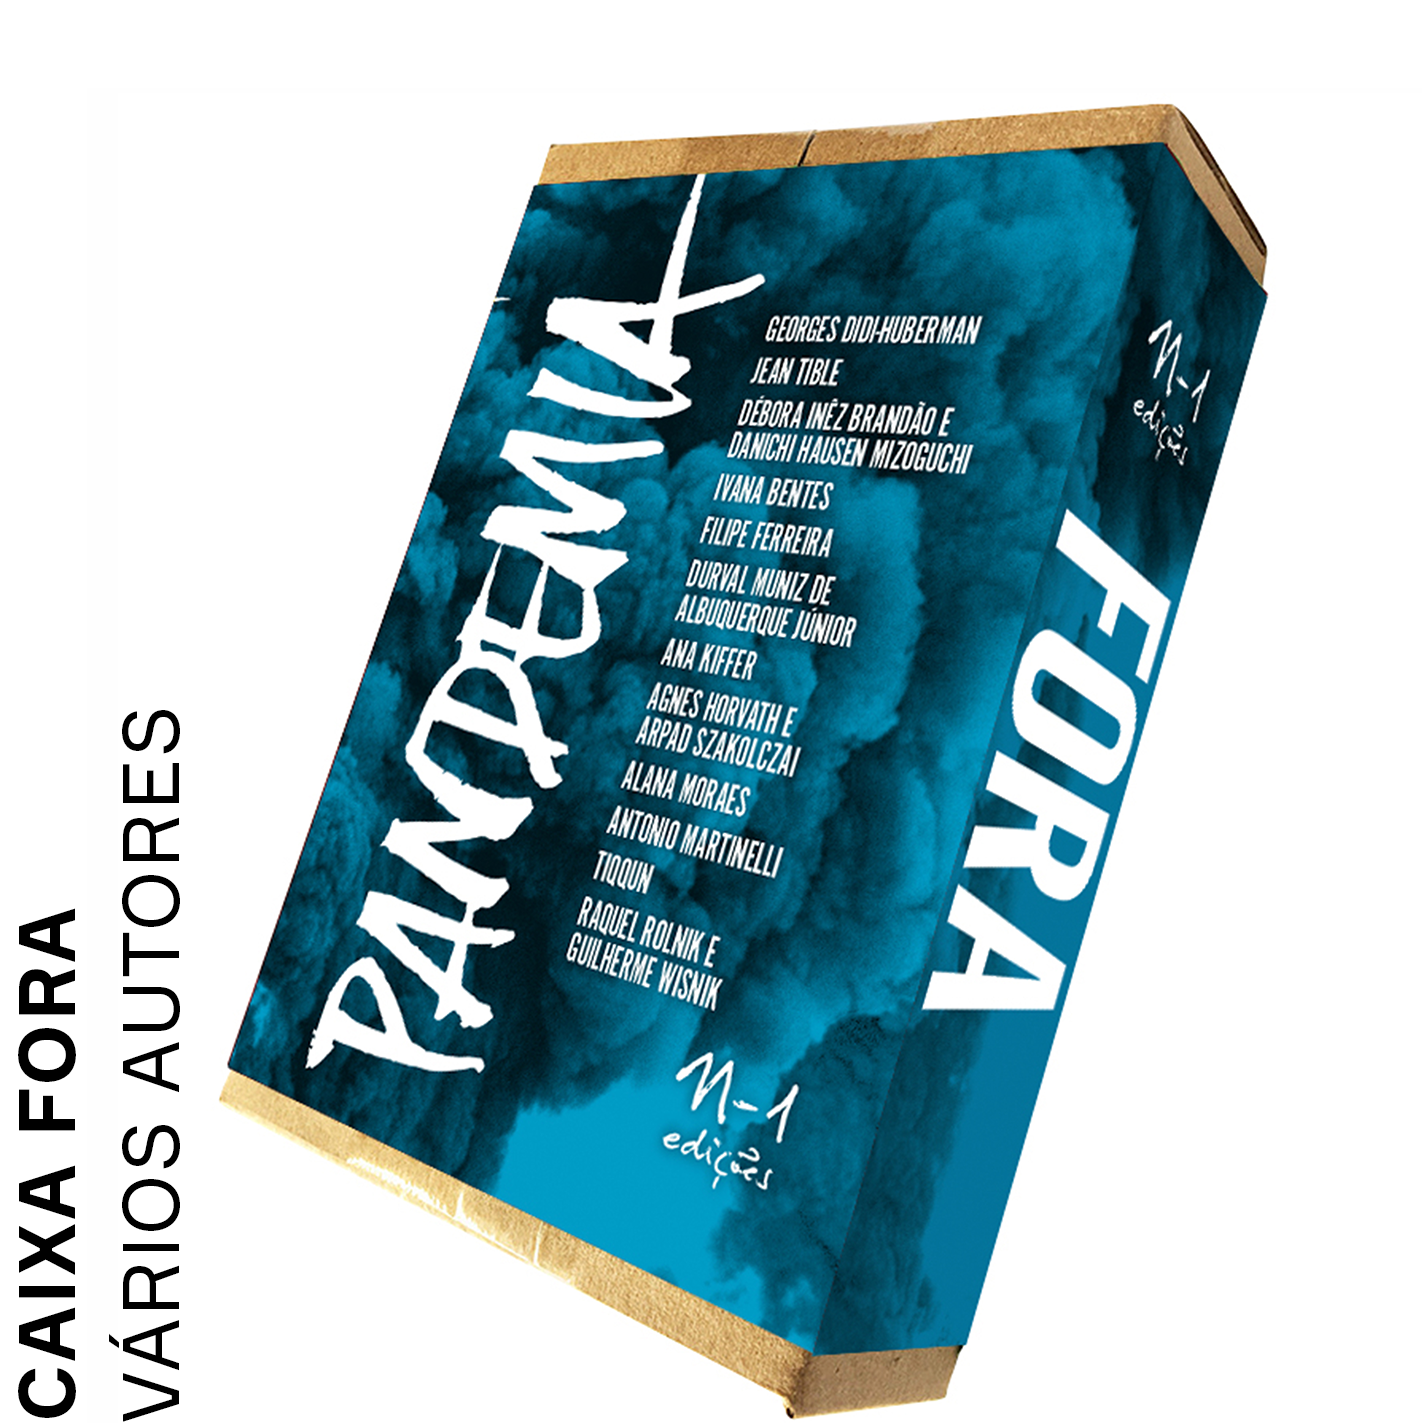
\includegraphics[width=40mm]{./GRID/N-1_CAIXA.png}}
\subfloat{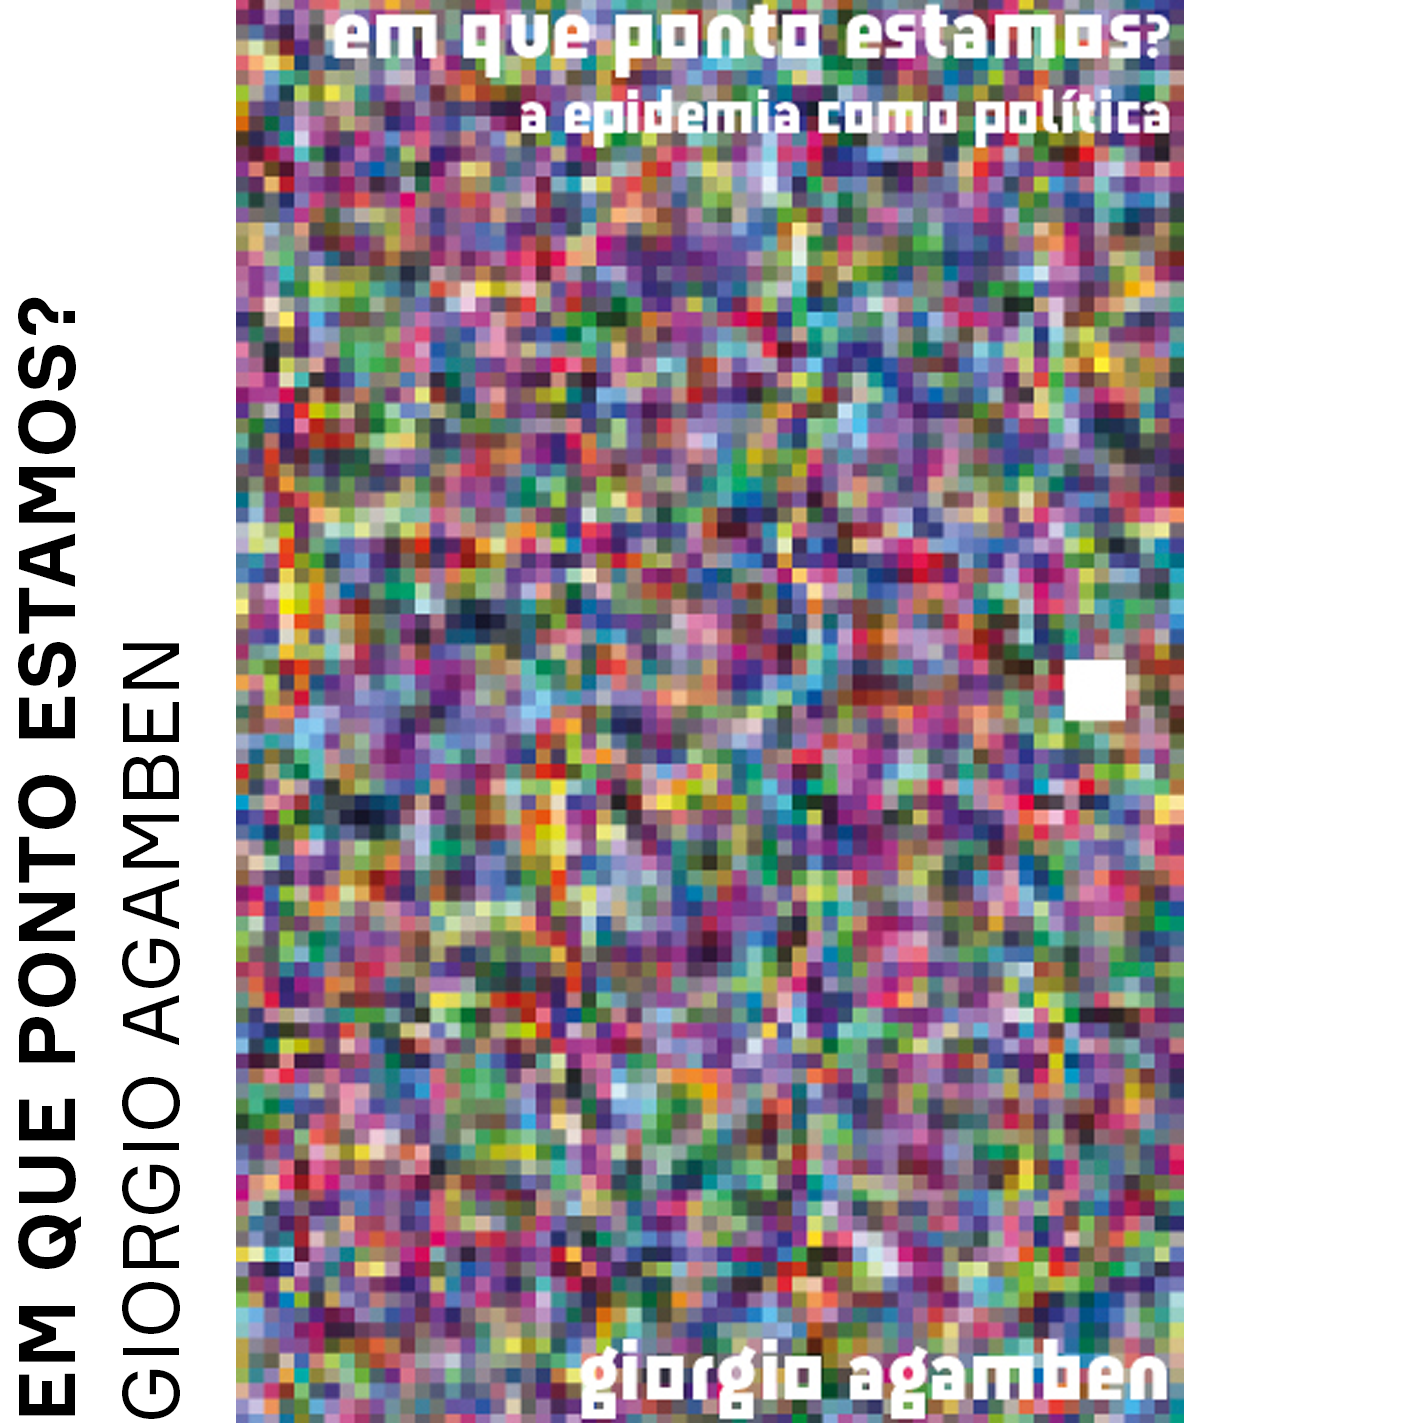
\includegraphics[width=40mm]{./GRID/N1_AGAMBEN.png}}
\subfloat{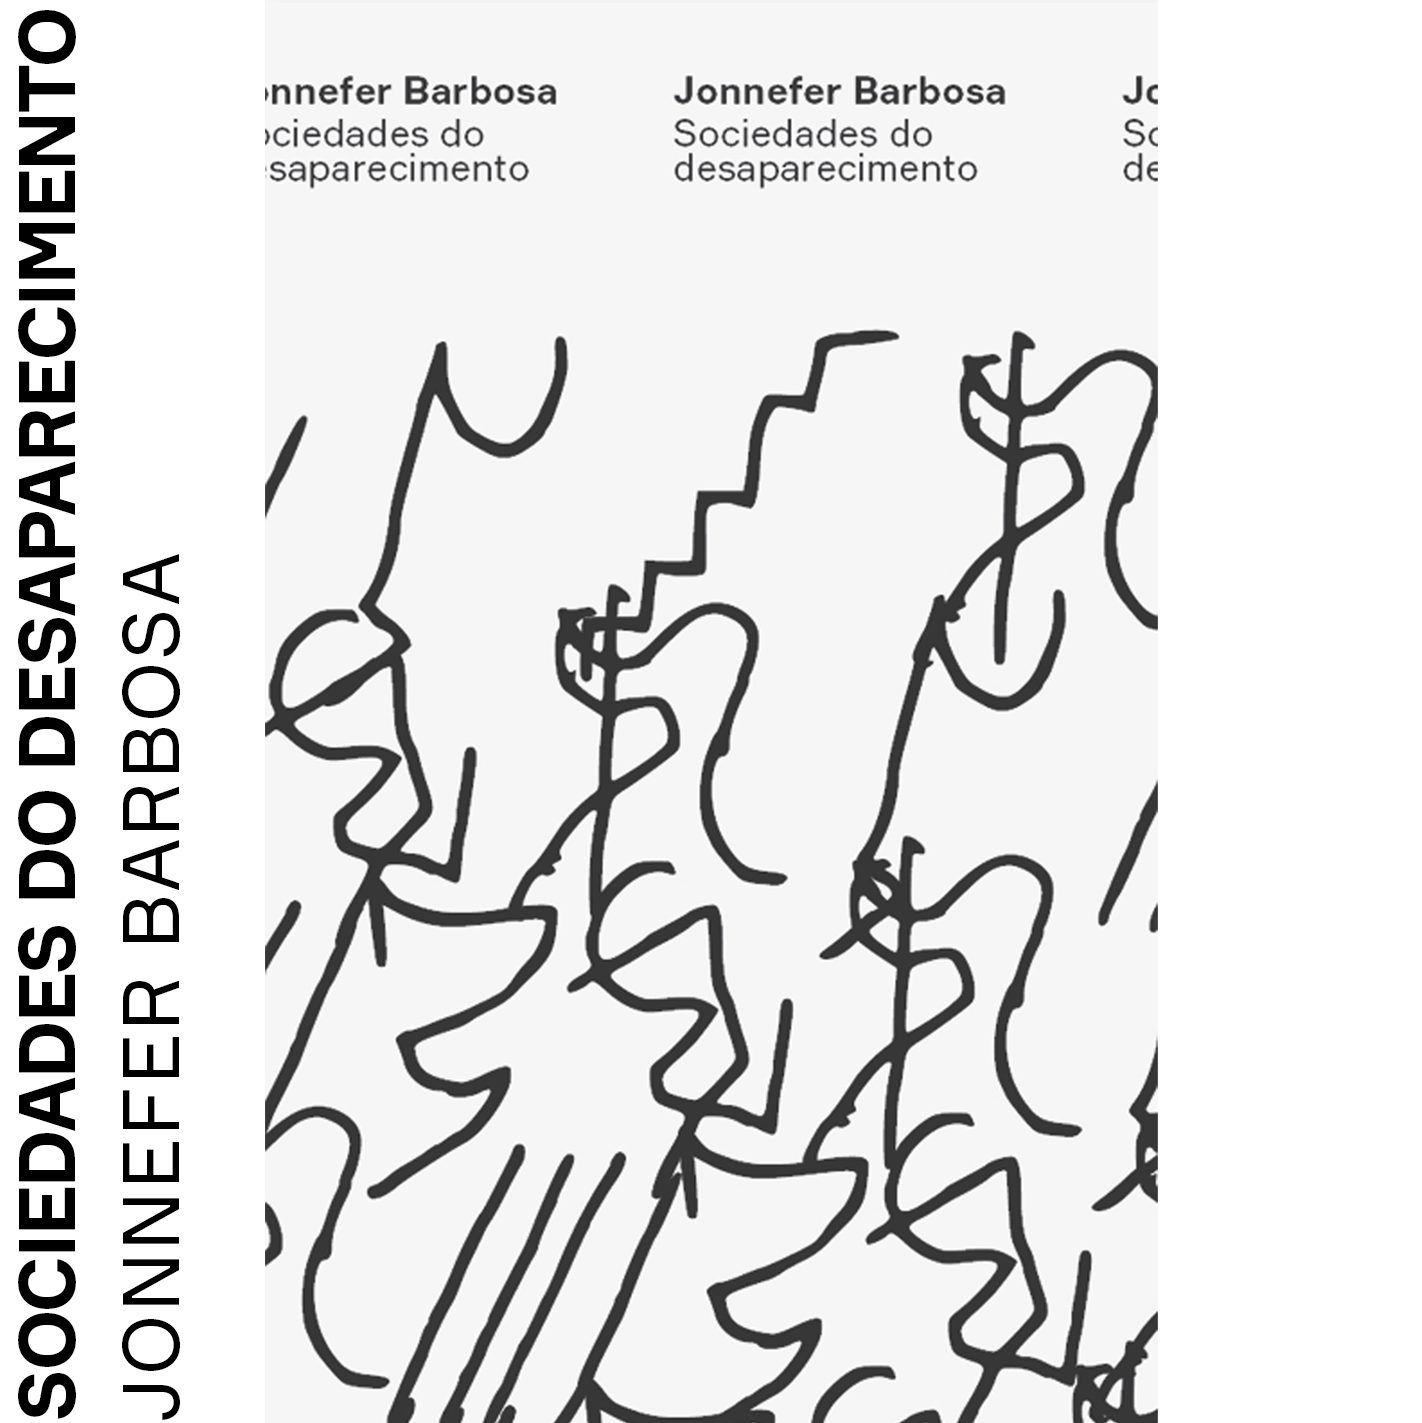
\includegraphics[width=40mm]{./GRID/N1_BARBOSA.png}}\\\hspace*{.5cm}

\vspace{.5cm}

\subfloat{
\includegraphics[width=40mm]{./GRID/N1_MBEMBE.png}}
\subfloat{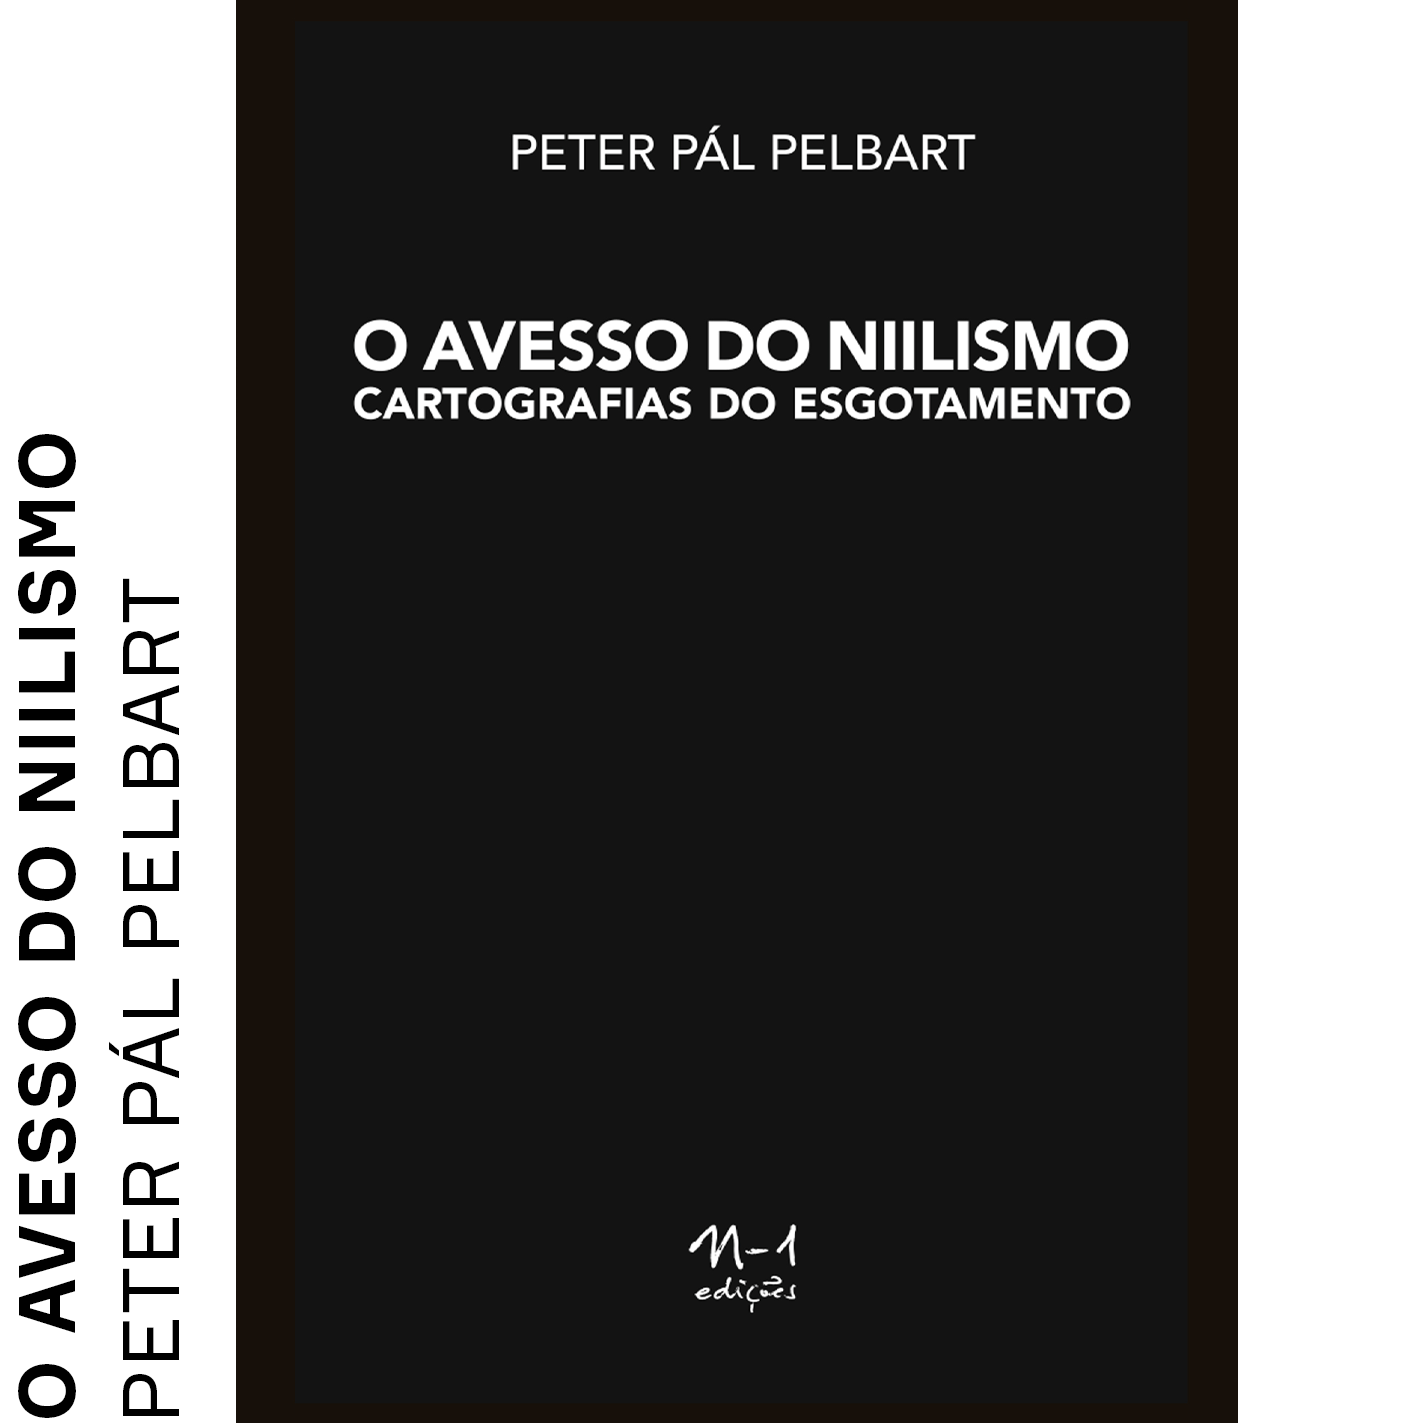
\includegraphics[width=40mm]{./GRID/N1_PELBART.png}}
\subfloat{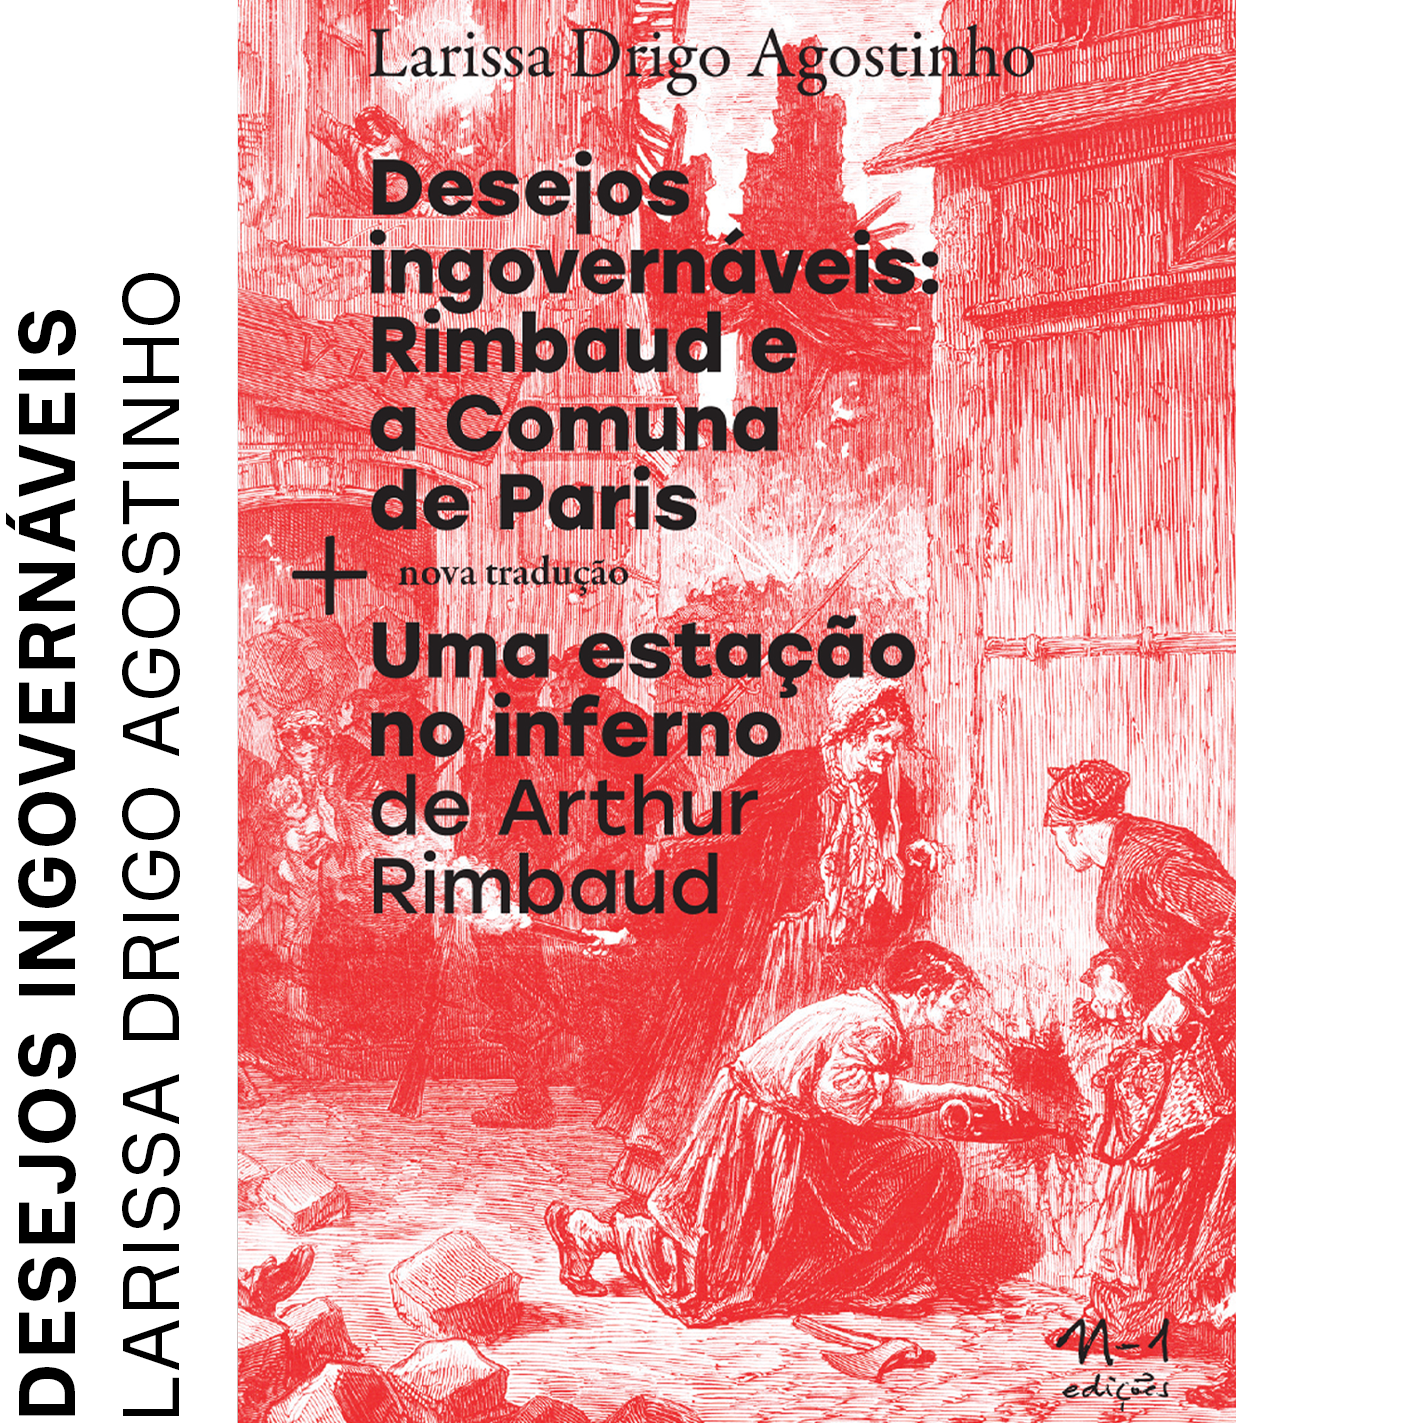
\includegraphics[width=40mm]{./GRID/N1_RIMBAUD.png}}\\\hspace*{.5cm}

\vspace{.5cm}

\subfloat{
\includegraphics[width=40mm]{./GRID/N1_TRATADO.png}}
\subfloat{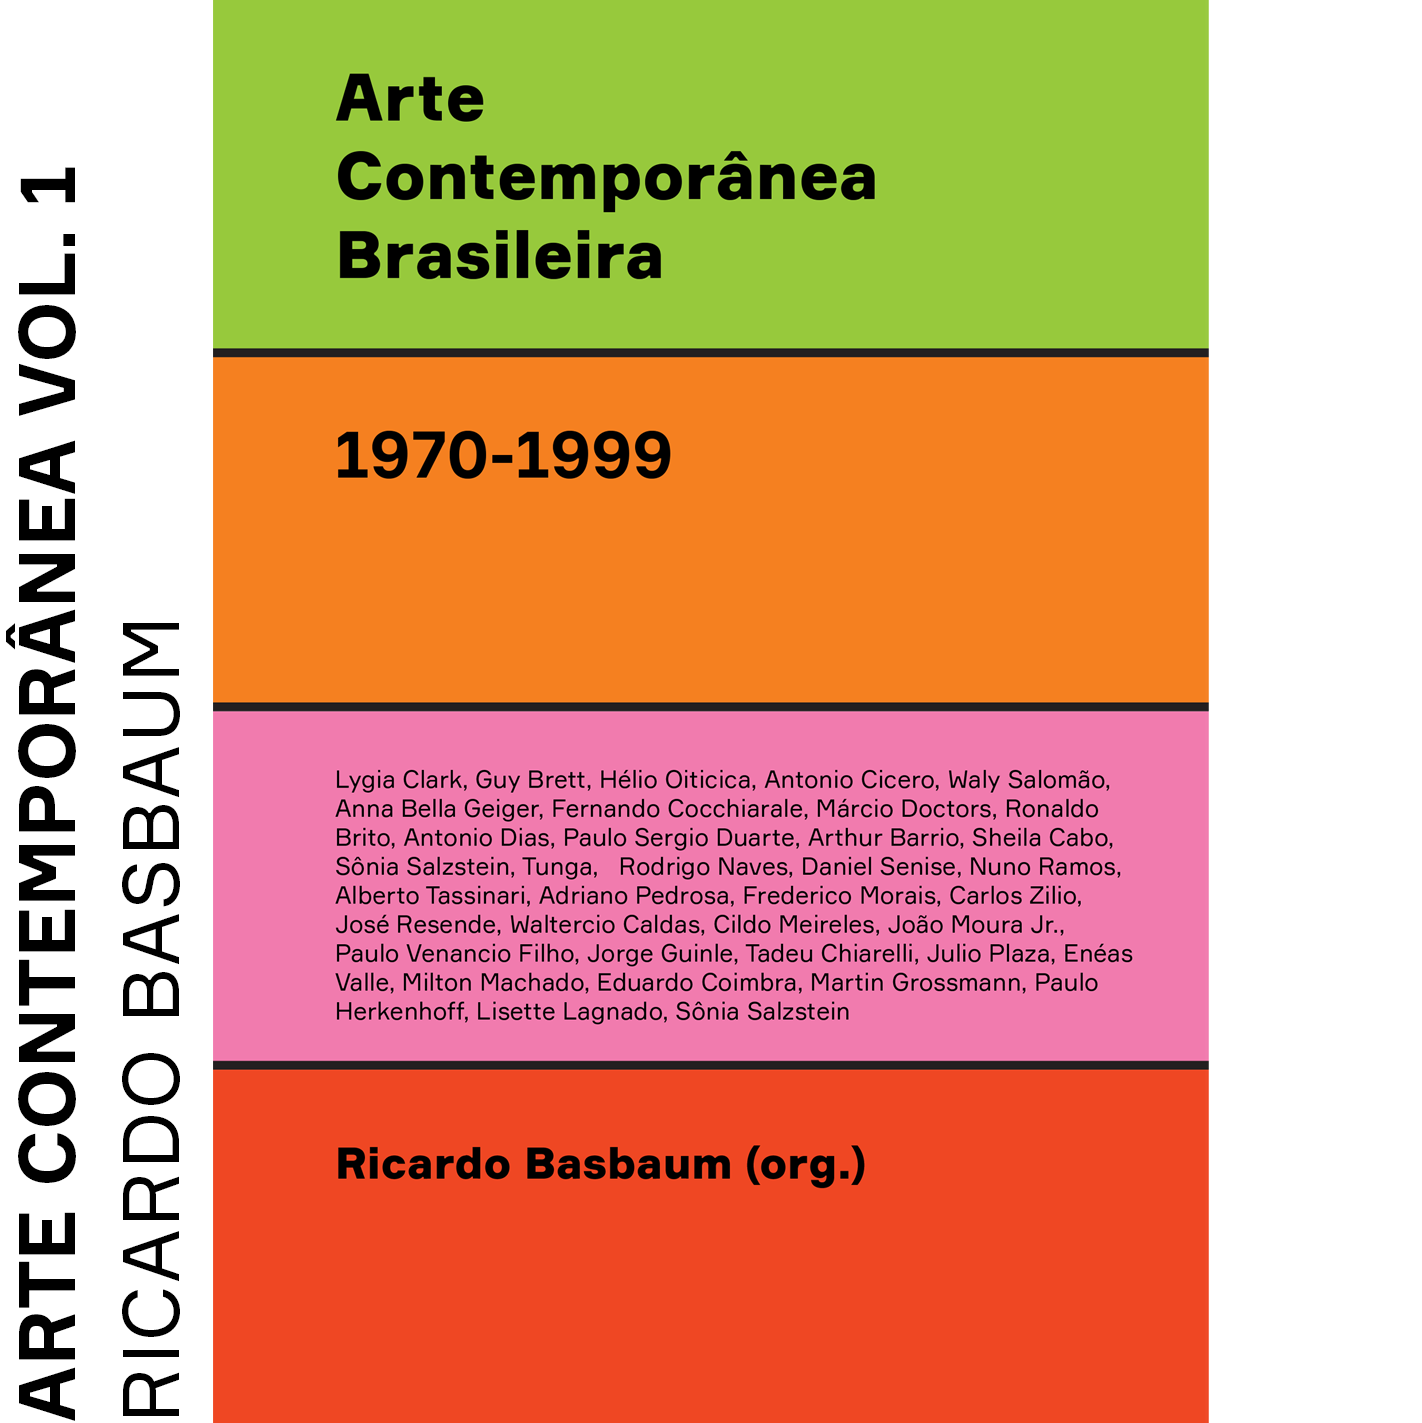
\includegraphics[width=40mm]{./GRID/CIRCUITO_BASBAUM.png}}
\subfloat{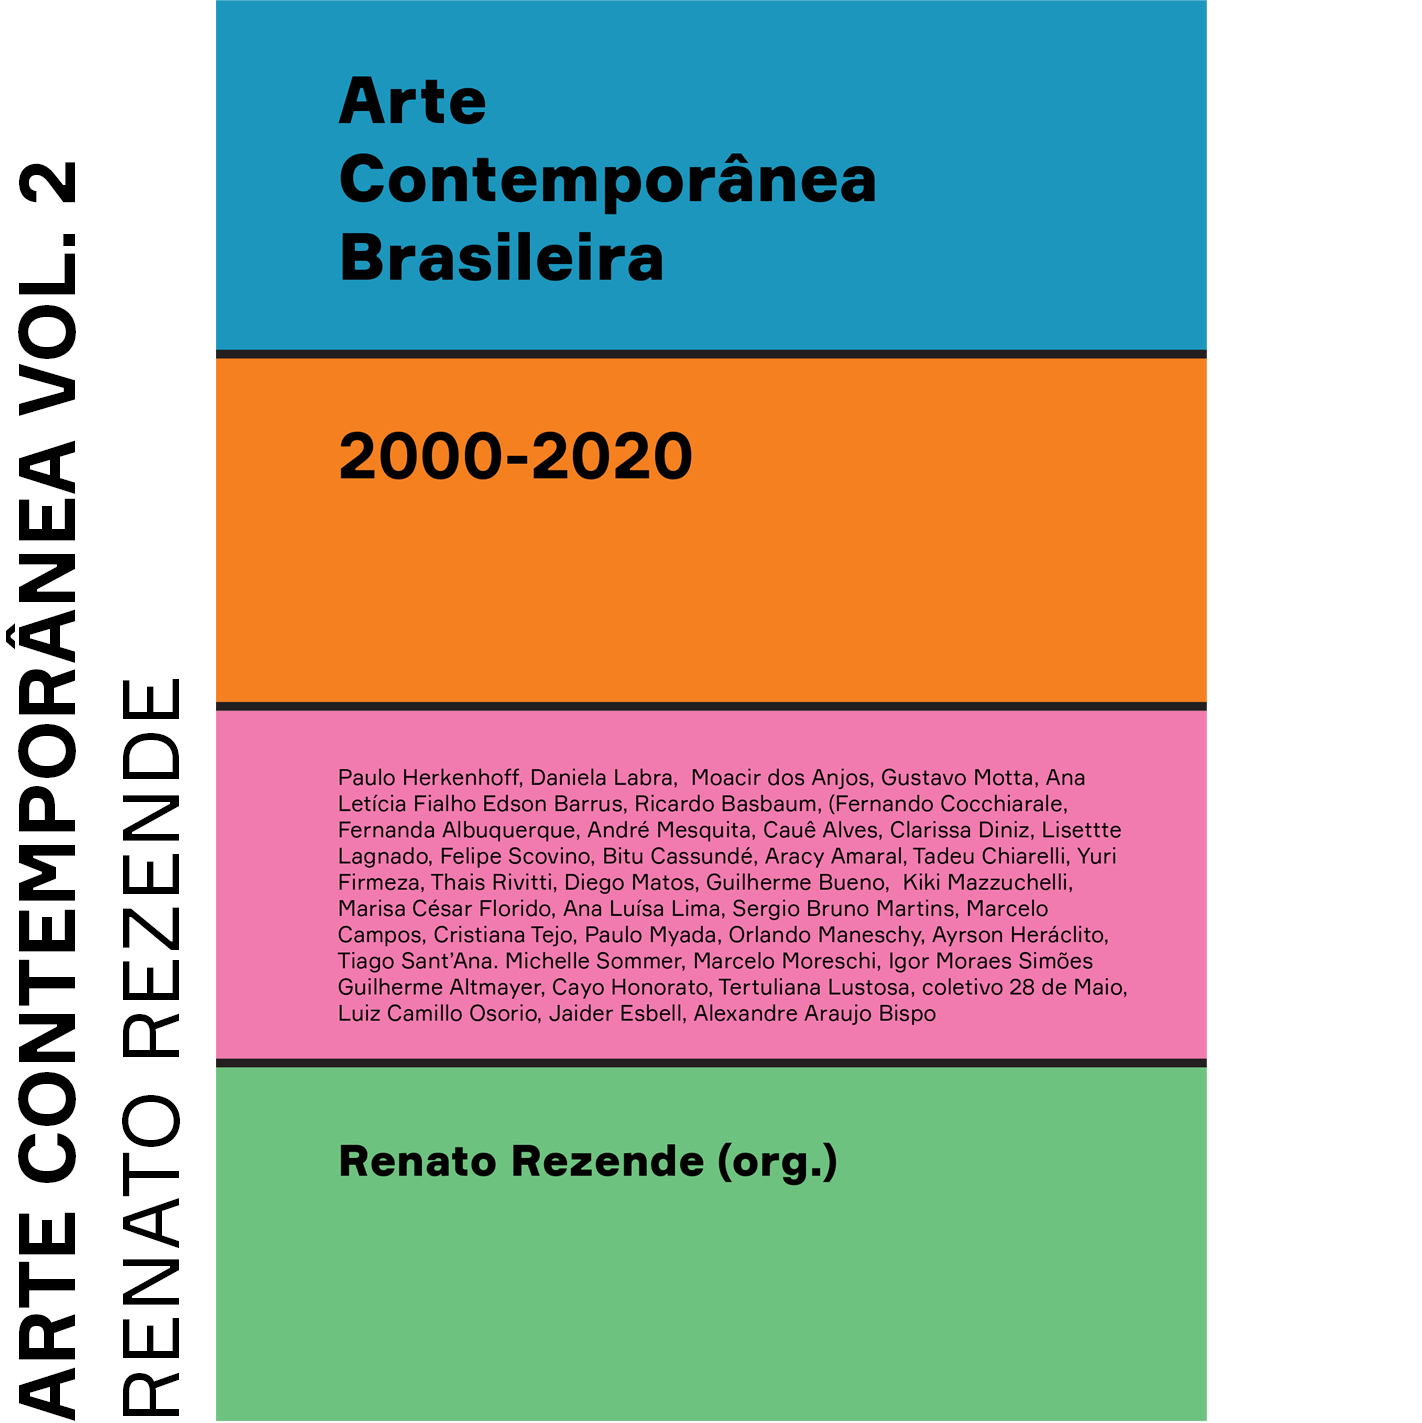
\includegraphics[width=40mm]{./GRID/CIRCUITO_REZENDE.png}}\\\hspace*{.5cm}
\end{tabular}
\end{figure}
\pagebreak

\pagestyle{grid}
\begin{figure}[!htbp]
\begin{tabular}{cccc}
\vspace{.5cm}
\hspace*{.5cm}
\subfloat{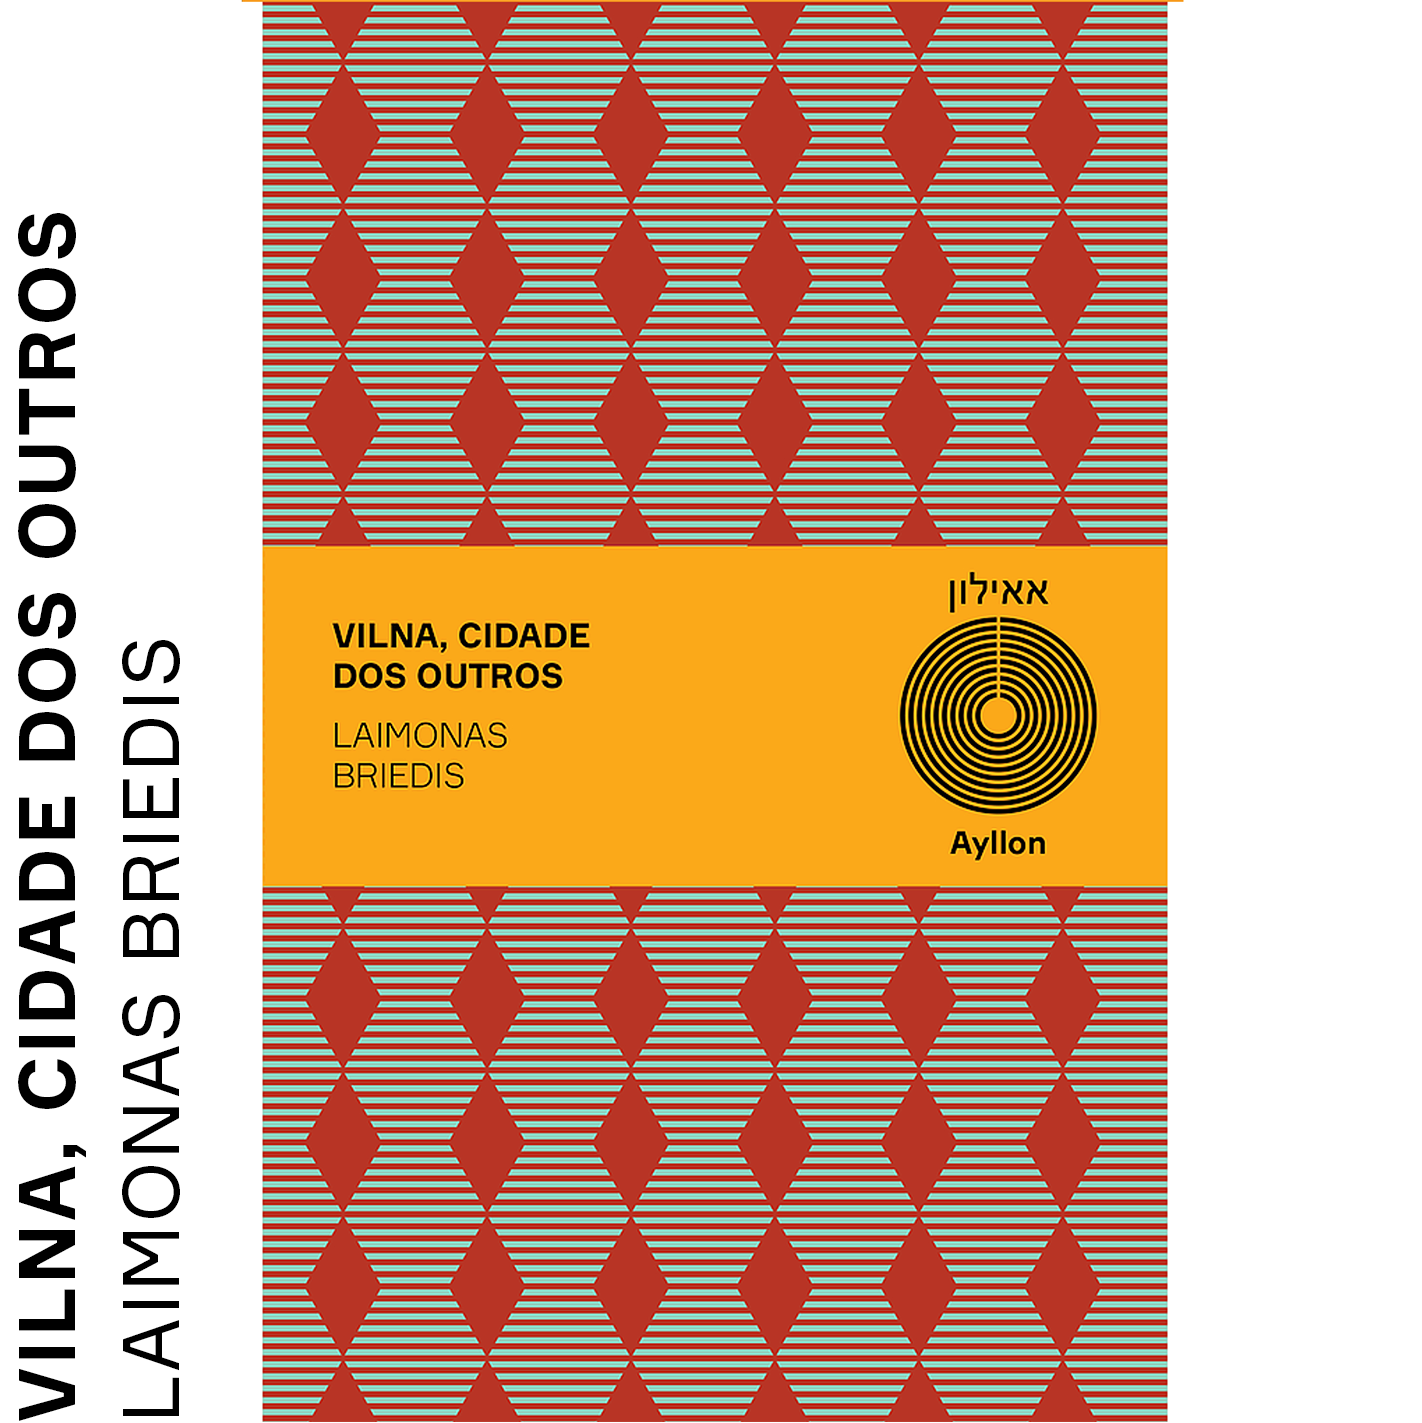
\includegraphics[width=40mm]{./GRID/AYLLON_VILNA.png}}
\subfloat{
\includegraphics[width=40mm]{./GRID/AYLLON_BLECHER.png}}
\subfloat{
\includegraphics[width=40mm]{./GRID/AYLLON_AMERICA.png}}\\\hspace*{.5cm}

\vspace{.5cm}

\subfloat{
\includegraphics[width=40mm]{./GRID/ACORDE_TATIT.png}}
\subfloat{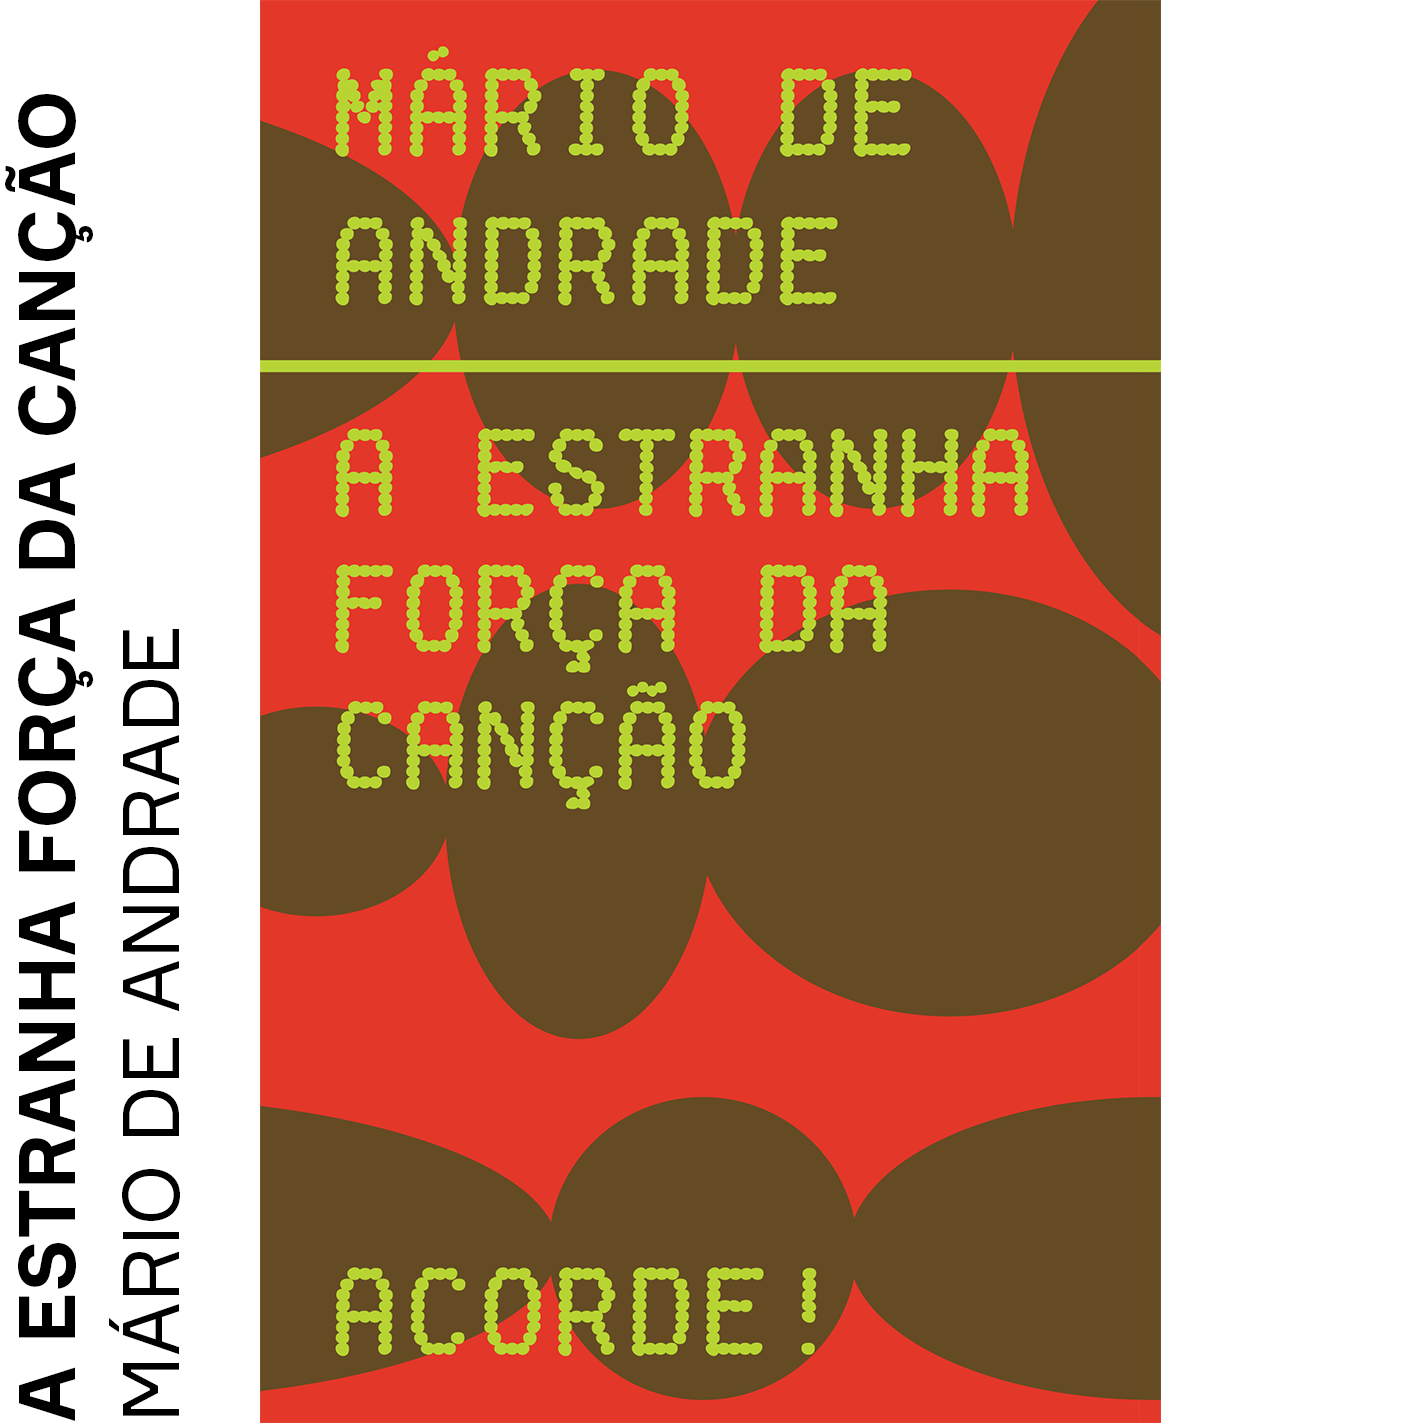
\includegraphics[width=40mm]{./GRID/ACORDE_MARIO.png}}\\\hspace*{.5cm}
\end{tabular}
\end{figure}
\pagebreak
\blankpage

\blankpage

\pagestyle{hedra}
\label{hedra}
%\begin{textblock*}{5.625in}(0pt,0pt)%
%\vspace*{-3.5cm}
%\hspace*{-2.77cm}\includegraphics*[width=175.2mm]{./propagandas/HEDRA.pdf}
%\end{textblock*}
%\pagebreak

\begin{center}
\hspace*{-3.6cm}\raisebox{5cm}{\rotatebox[origin=t]{90}{\huge\textbf{Lançamento}}}
\hspace*{3.1cm}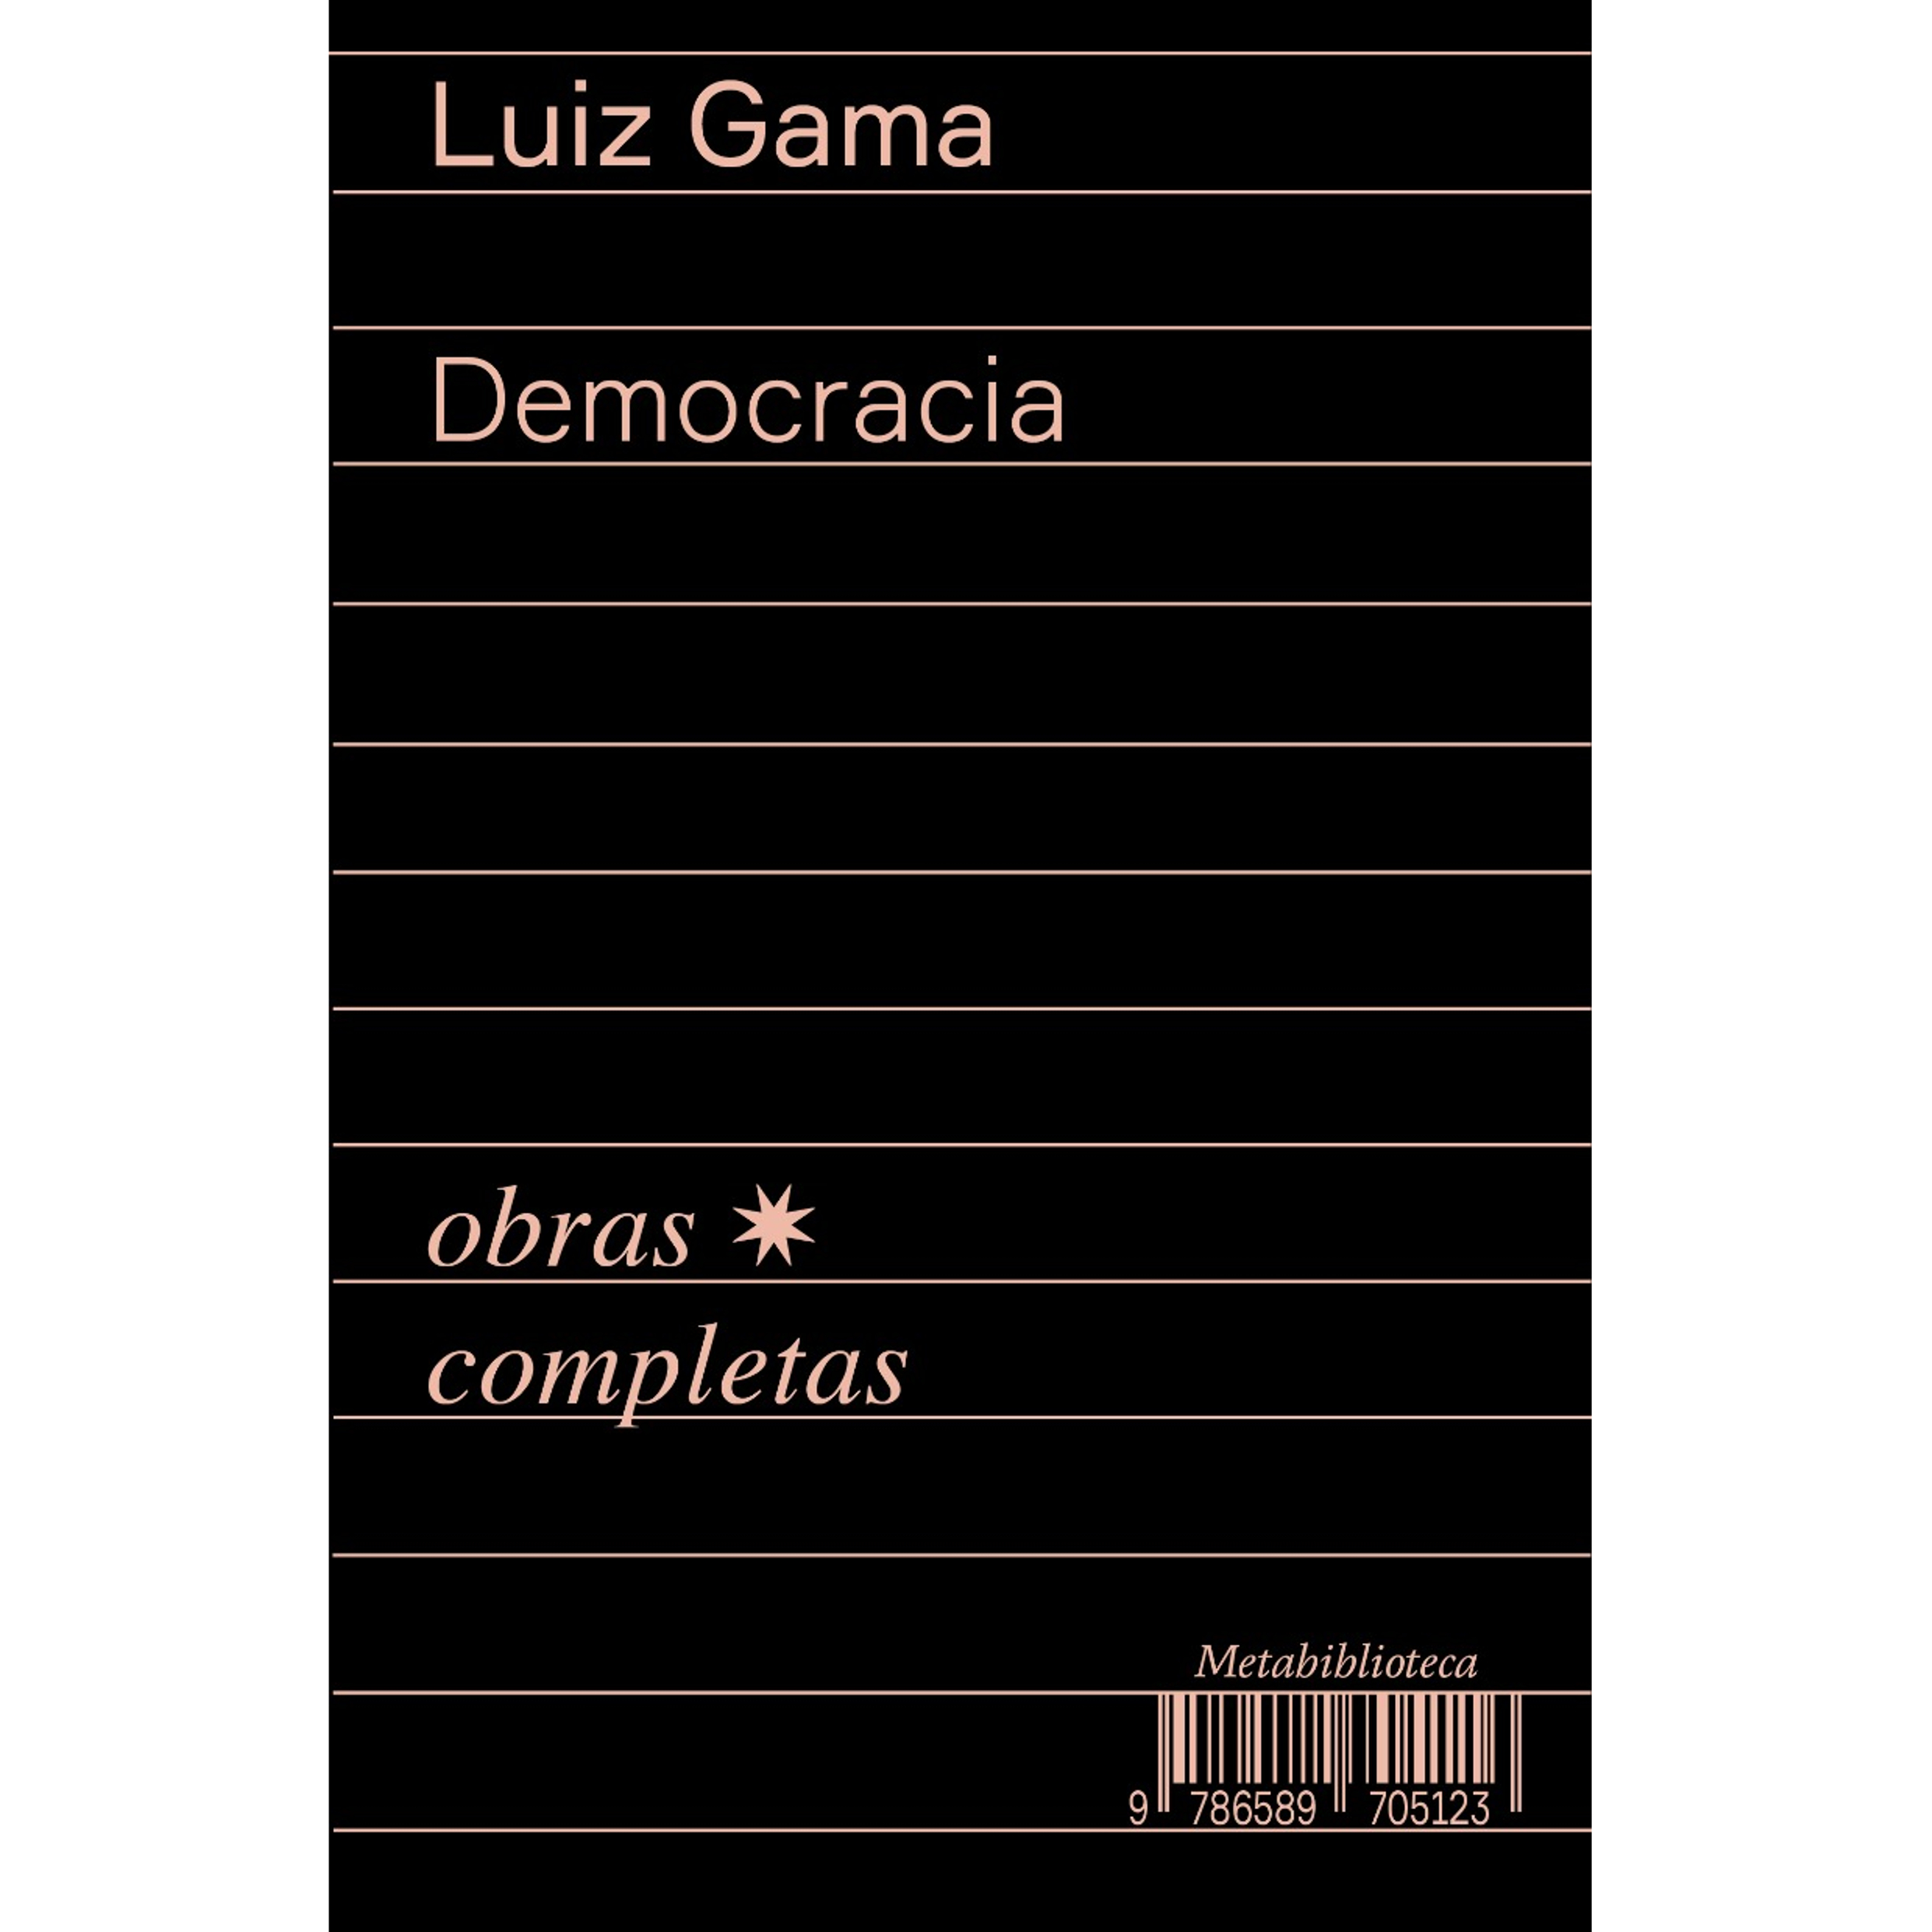
\includegraphics[width=74mm]{./CAPAS/HEDRA_DEMOCRACIA.jpg}
\end{center}
\hspace*{-7cm}\hrulefill\hspace*{-7cm}
\medskip

\noindent{}Os textos e artigos incluídos em \textit{Democracia} foram publicados originalmente entre os anos de 1866 e 1869. Nesses artigos, Luiz Gama se manifesta publicamente sobre educação, política e direitos universais. \hlc{Lançando mão de uma estratégia autoral ousada, que incluía o uso de pseudônimos, Gama defende abertamente o direito à educação universal e as obrigações do Estado em garantir um ensino público de qualidade} em todos os níveis como os fundamentos da vida democrática.

\textit{Democracia} integra as \textit{Obras completas} de Luiz Gama, advogado negro e abolicionista, a serem lançadas em 11 volumes com cerca de 800 escritos --- 600 inéditos ---, revelando as diversas facetas e estilos empregados pelo escritor para advogar pela grande causa de sua vida: a abolição da escravidão e a emancipação negra. Esquecidos em parte por quase dois séculos, os textos foram recuperados pelo pesquisador Bruno Rodrigues de Lima, que passou nove anos localizando-os em arquivos da imprensa e do judiciário de todo o país.

\vfill
\noindent\begin{minipage}[c]{1\linewidth}
{\small\textbf{
\hspace*{-.1cm}Editora: Hedra\\
Título: Democracia (1866--1869)\\
Autor: Luiz Gama\\ 
ISBN: 978-65-89705-12-3\\
Páginas: 506\\
Formato: 13,3x21\,cm\\
Preço: R\$ 110,00\\
}}
\end{minipage}
\pagebreak

\begin{center}
\hspace*{.5cm}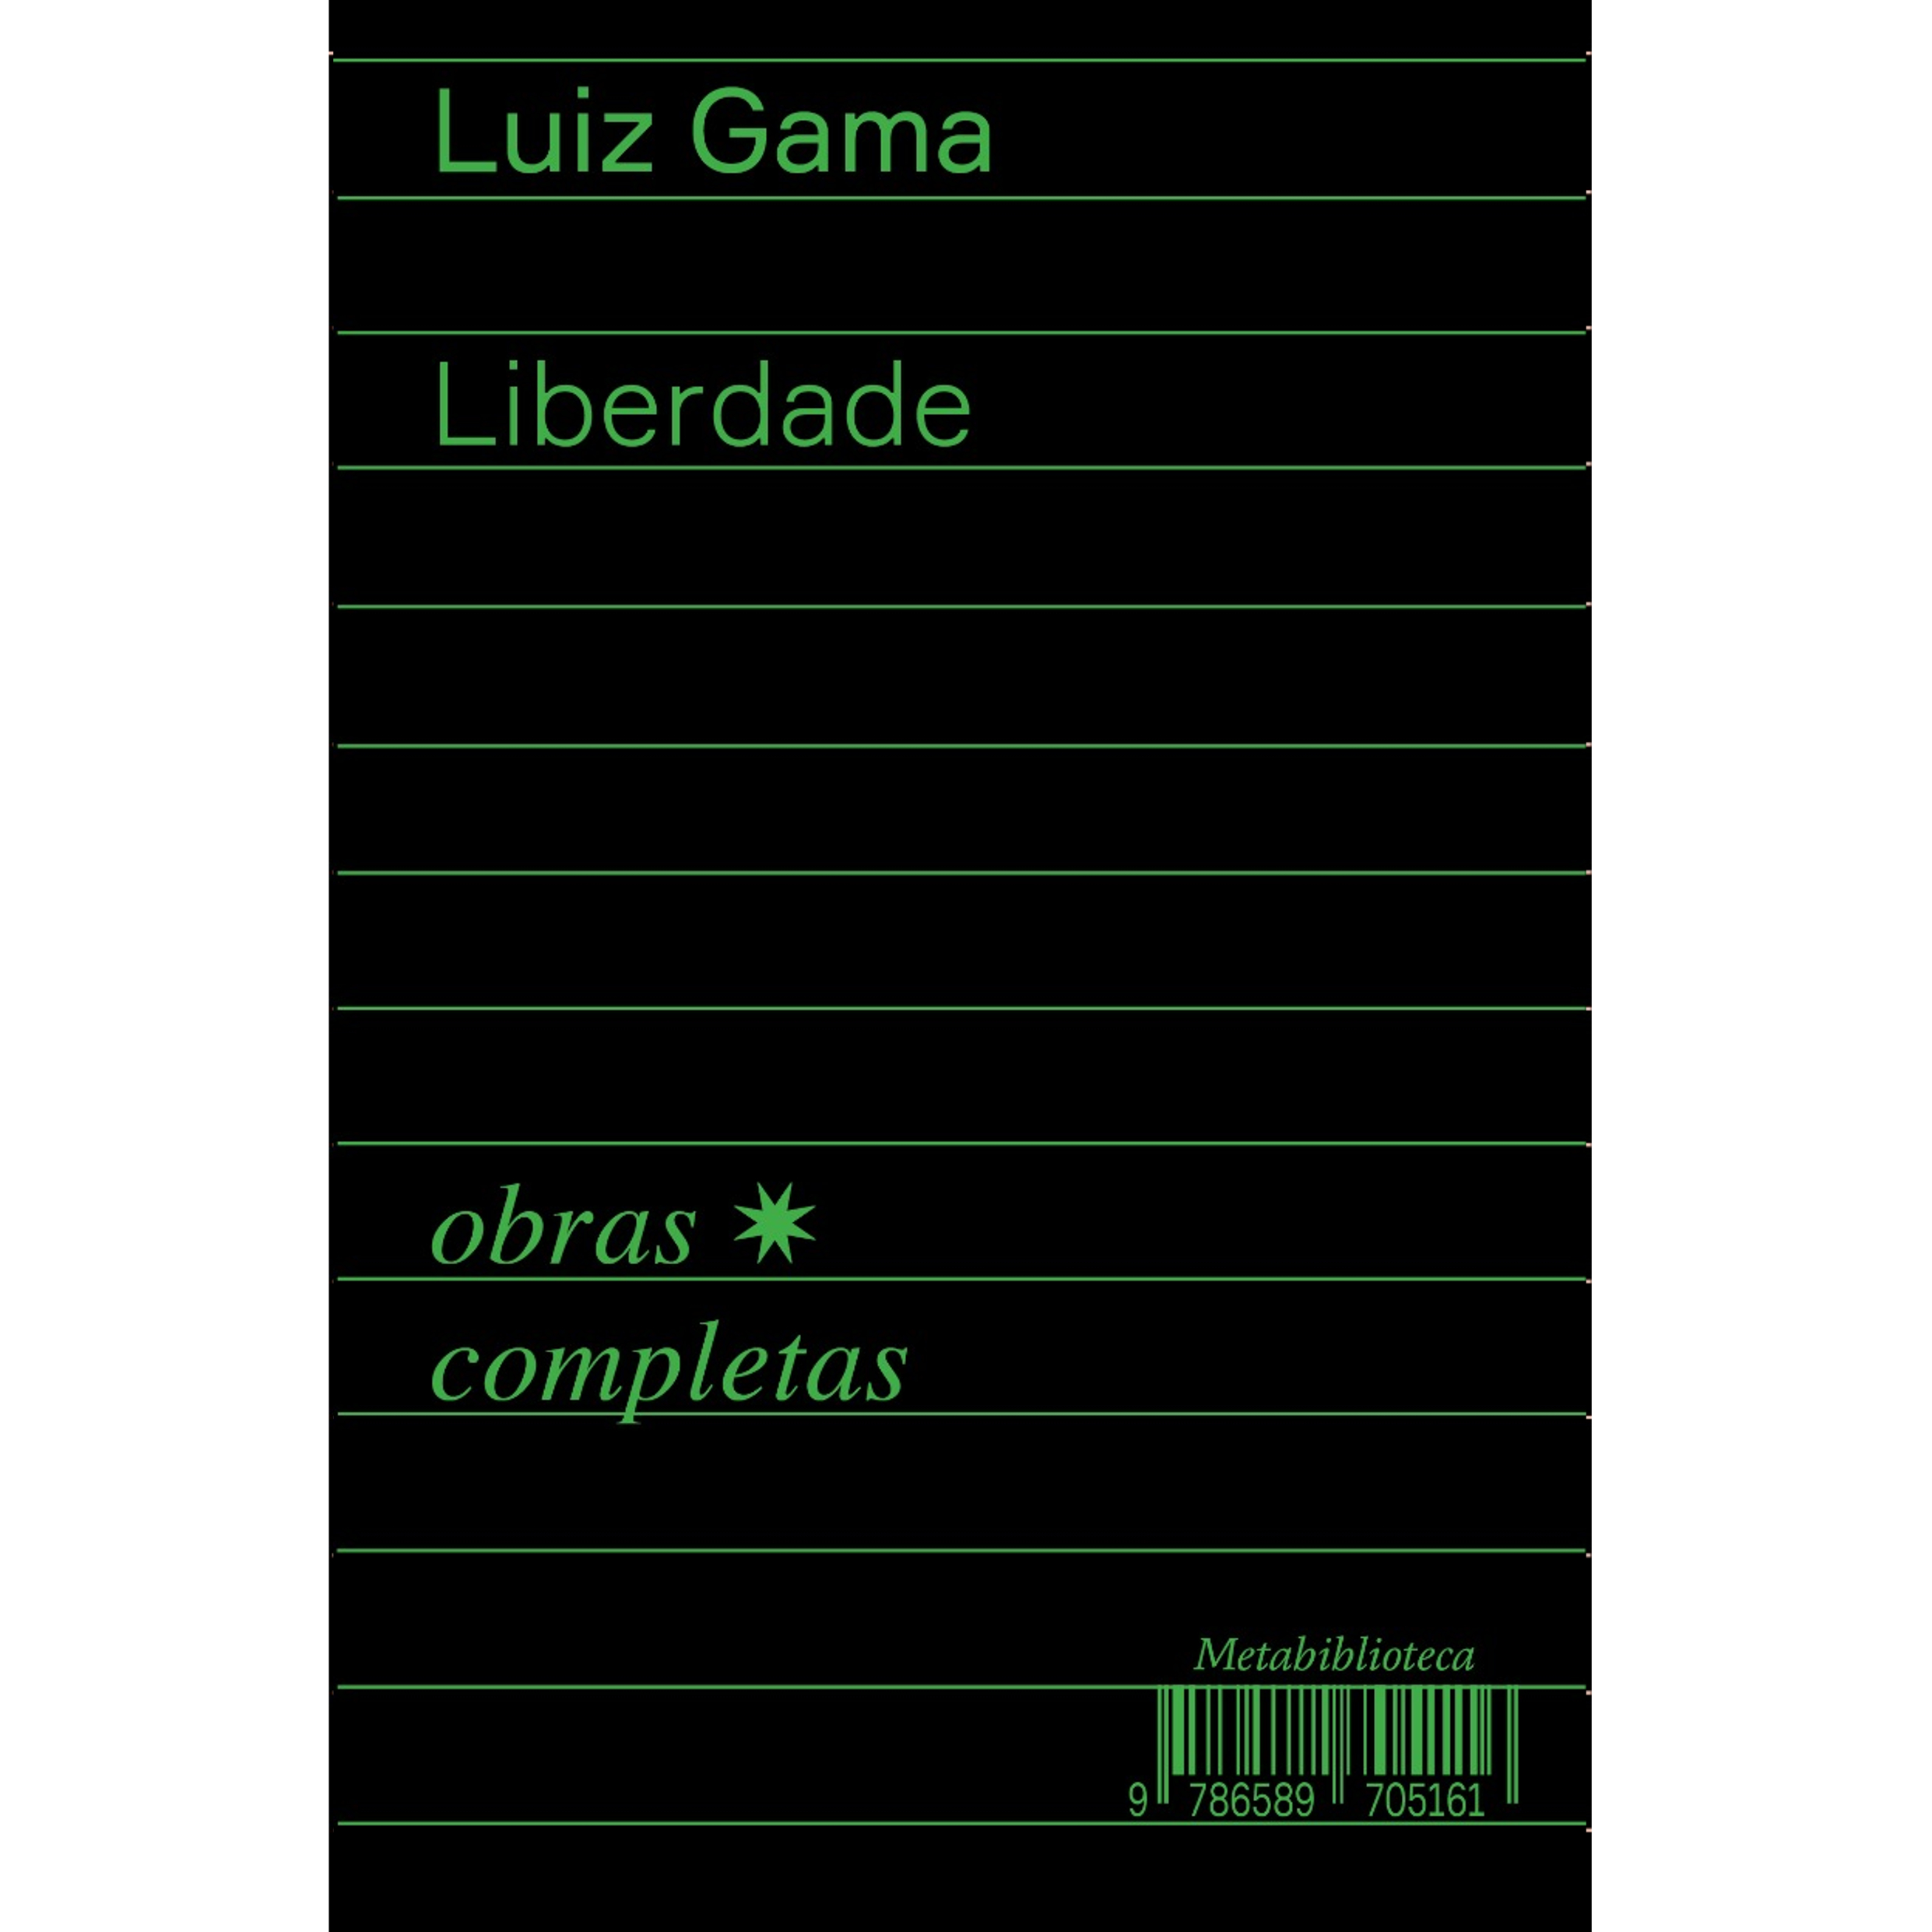
\includegraphics[width=74mm]{./CAPAS/HEDRA_LIBERDADE.jpg}
\end{center}
\hspace*{-7cm}\hrulefill\hspace*{-7cm}
\medskip

\noindent{}Os textos deste volume são \hlc{fruto da campanha pela abolição radical, que também visava à garantia da educação e cidadania para os libertos: o abolicionismo de Gama exigia cidadania e igualdade de fato e de direito}. O advogado também refletia sobre o processo histórico em curso, e propunha soluções políticas para o tempo presente, revelando sua natureza intelectual até hoje pouco conhecida e quase sempre não reconhecida.

\textit{Liberdade} integra as \textit{Obras completas} de Luiz Gama, advogado negro e abolicionista, a serem lançadas em 11 volumes com cerca de 800 escritos --- 600 inéditos ---, revelando as diversas facetas e estilos empregados pelo escritor para advogar pela grande causa de sua vida: a abolição da escravidão e a emancipação negra. Esquecidos em parte por quase dois séculos, os textos foram recuperados pelo pesquisador Bruno Rodrigues de Lima, que passou nove anos localizando-os em arquivos da imprensa e do judiciário de todo o país.

\vfill
\noindent\begin{minipage}[c]{.5\linewidth}
{\small\textbf{
\hspace*{-.1cm}Editora: Hedra\\
Título: Liberdade (1880--1882)\\
Autor: Luiz Gama\\ 
ISBN: 978-65-89705-16-1\\
Páginas: 446\\
Formato: 13,3x21\,cm\\
Preço: R\$ 99,90\\
}}
\end{minipage}
\pagebreak

\begin{center}
\hspace*{-3.6cm}\raisebox{5cm}{\rotatebox[origin=t]{90}{\huge\textbf{Lançamento}}}
\hspace*{3.1cm}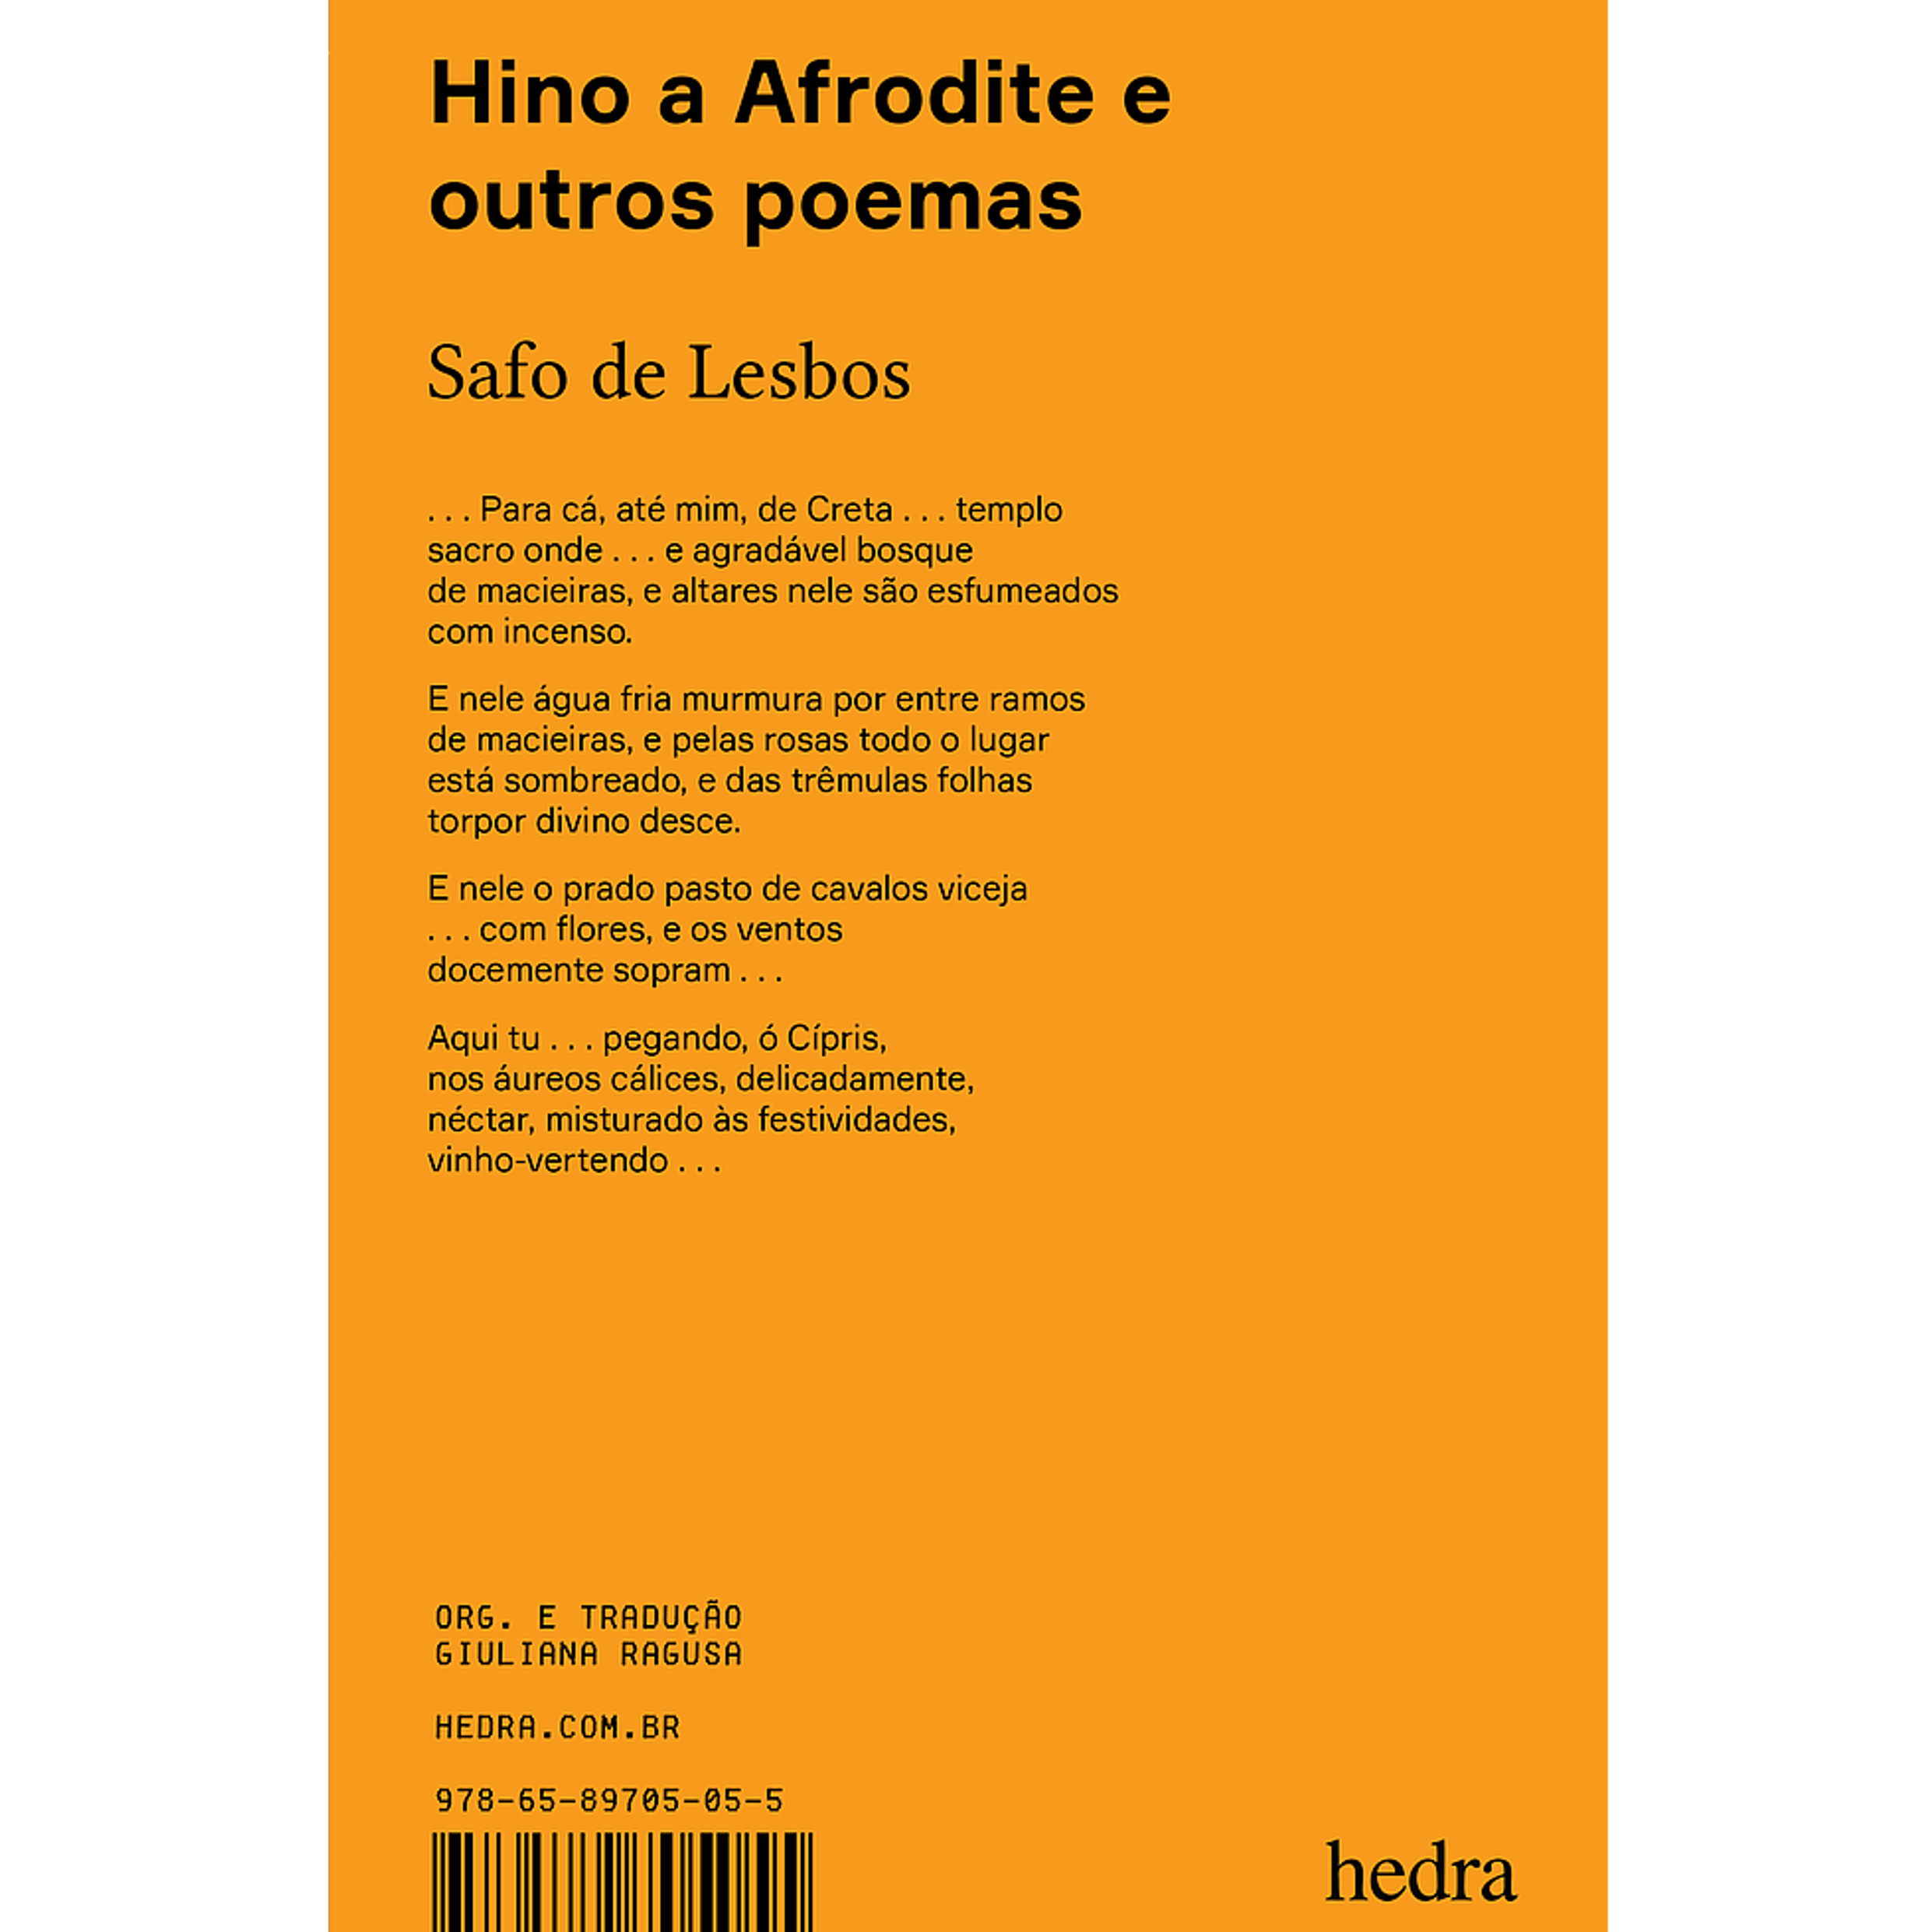
\includegraphics[width=74mm]{./CAPAS/HEDRA_SAFO.jpg}
\end{center}
\hspace*{-7cm}\hrulefill\hspace*{-7cm}
\medskip

\noindent{}Reunião de \hlc{textos remanescentes da mélica de Safo, ou seja, as canções para performance ao som da lira. Os textos aqui são traduzidos e anotados por Giuliana Ragusa em segunda edição --- com novos poemas, atualizações e em versão bilíngue} ---, autora que ganhou o Jabuti 2006 com um livro sobre a lírica da poeta, a única mulher entre os grandes da época. Para esta edição foram selecionados a única canção completa e os fragmentos mais legíveis de canções do corpus de Safo. As anotações de leitura buscam lançar luz sobre elementos relevantes da estrutura, conteúdo ou transmissão dos fragmentos organizados tematicamente. Precede a tradução anotada uma introdução sobre a poeta, sua poesia e o contexto em que se produziu e circulou, o gênero mélico, a fortuna crítica sobre ela, a transmissão de sua obra, e as outras poetas mulheres de que se tem notícia.

\vfill
\noindent\begin{minipage}[c]{1\linewidth}
{\small\textbf{
\hspace*{-.1cm}Editora: Hedra\\
Título: Hino a Afrodite e outros poemas\\
Autor: Safo de Lesbos\\ 
ISBN: 978-65-89705-05-5\\
Páginas: 212\\
Formato: 13,3x21\,cm\\
Preço: R\$ 69,00\\
}}
\end{minipage}
\pagebreak

\begin{center}
\hspace*{.5cm}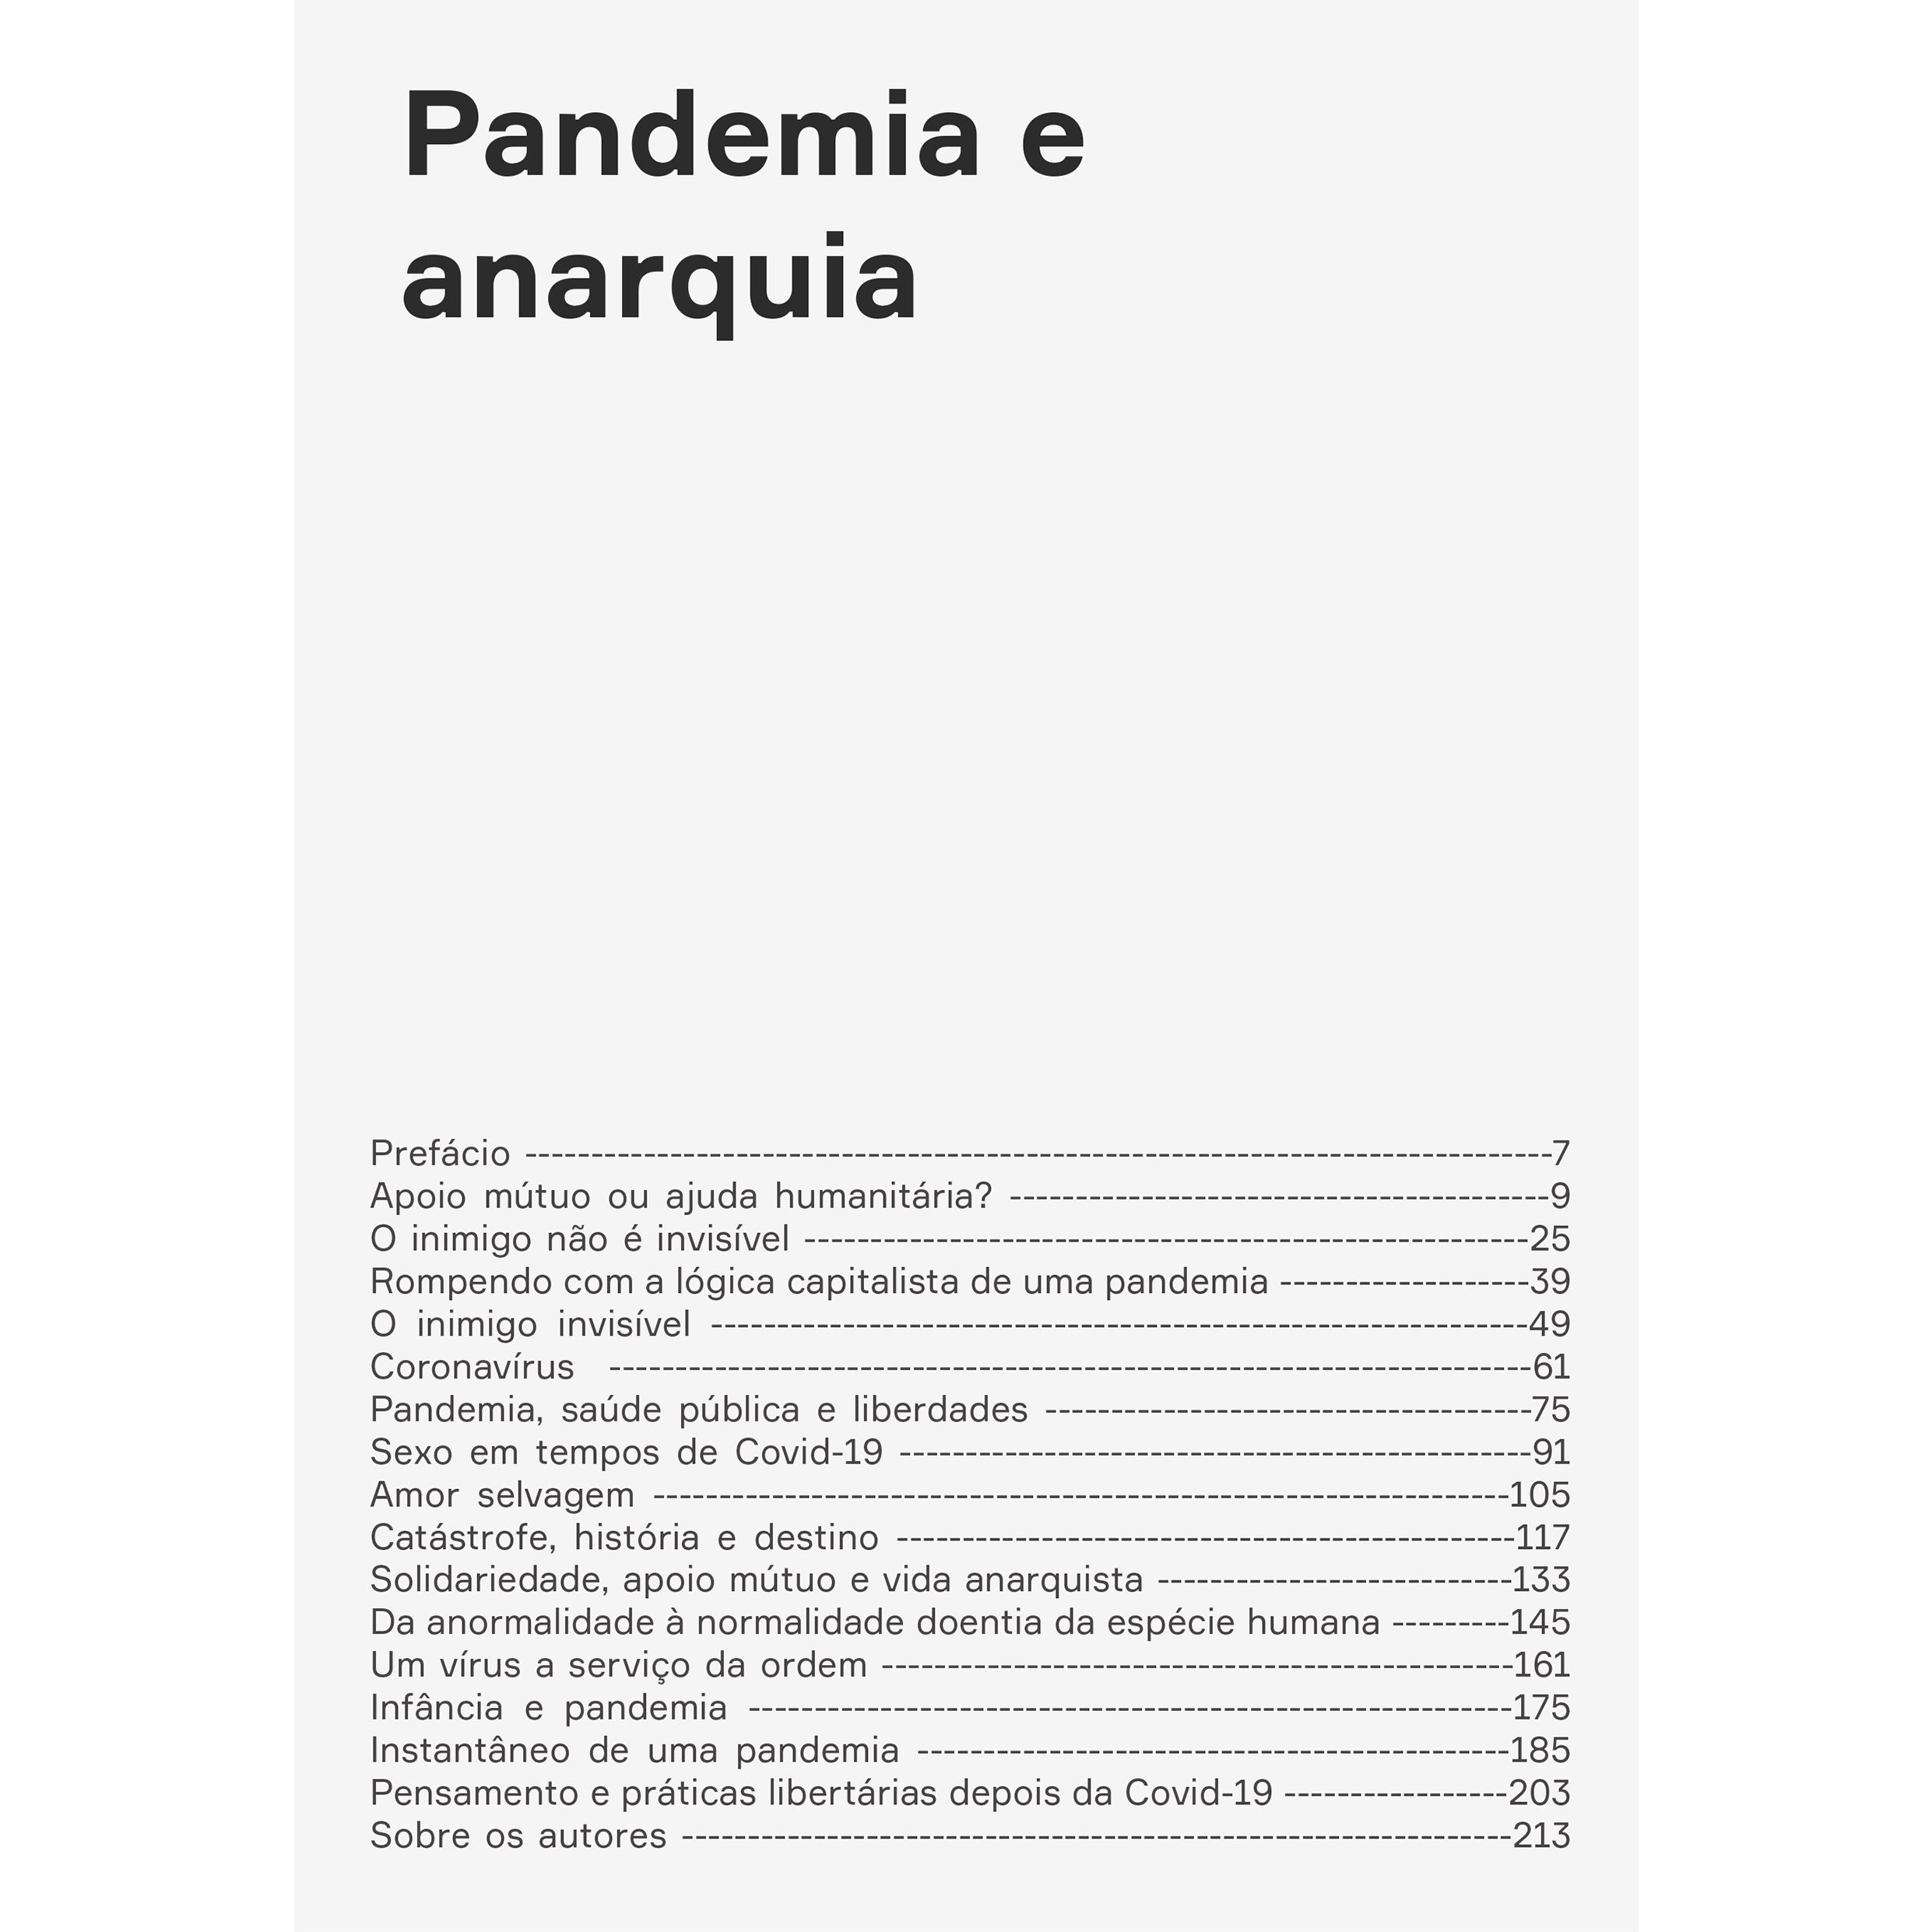
\includegraphics[width=74mm]{./CAPAS/HEDRA_PANDEMIA.jpg}
\end{center}
\hspace*{-7cm}\hrulefill\hspace*{-7cm}
\medskip

\noindent{}\textit{Pandemia e anarquia} reúne quinze ensaios de pesquisadores das práticas libertárias que analisam as implicações sociopolíticas do novo coronavírus e sua relação com os modos de existência. Além da Somaterapia e de pesquisadores do Nu-Sol (Núcleo de Sociabilidade Libertária), este livro traz escritos de historiadores e cientistas políticos residentes em diversos espaços do planeta. Perpassando diversas esferas das relações humanas, da economia e da ciência às relações amorosas e ao ser criança durante a pandemia, \hlc{os escritos insurgem-se contra a suposta ruptura com o mundo dado antes da Covid-19 para analisar e estancar a racionalidade neoliberal}, e a chamada crise sanitária. Com isso, traçam a afirmação de uma vida outra no presente.

\vfill
\noindent\begin{minipage}[c]{.5\linewidth}
{\small\textbf{
\hspace*{-.1cm}Editora: Hedra\\
Título: Pandemia e anarquia\\
Autor: Edson Passetti, João da Mata e José Maria Carvalho Ferreira (orgs.)\\ 
ISBN: 978-65-89705-04-8\\
Páginas: 220\\
Formato: 16x23\,cm\\
Preço: R\$ 69,00\\
}}
\end{minipage}
\pagebreak

\begin{center}
\hspace*{-3.6cm}\raisebox{5cm}{\rotatebox[origin=t]{90}{\huge\textbf{Lançamento}}}
\hspace*{3.1cm}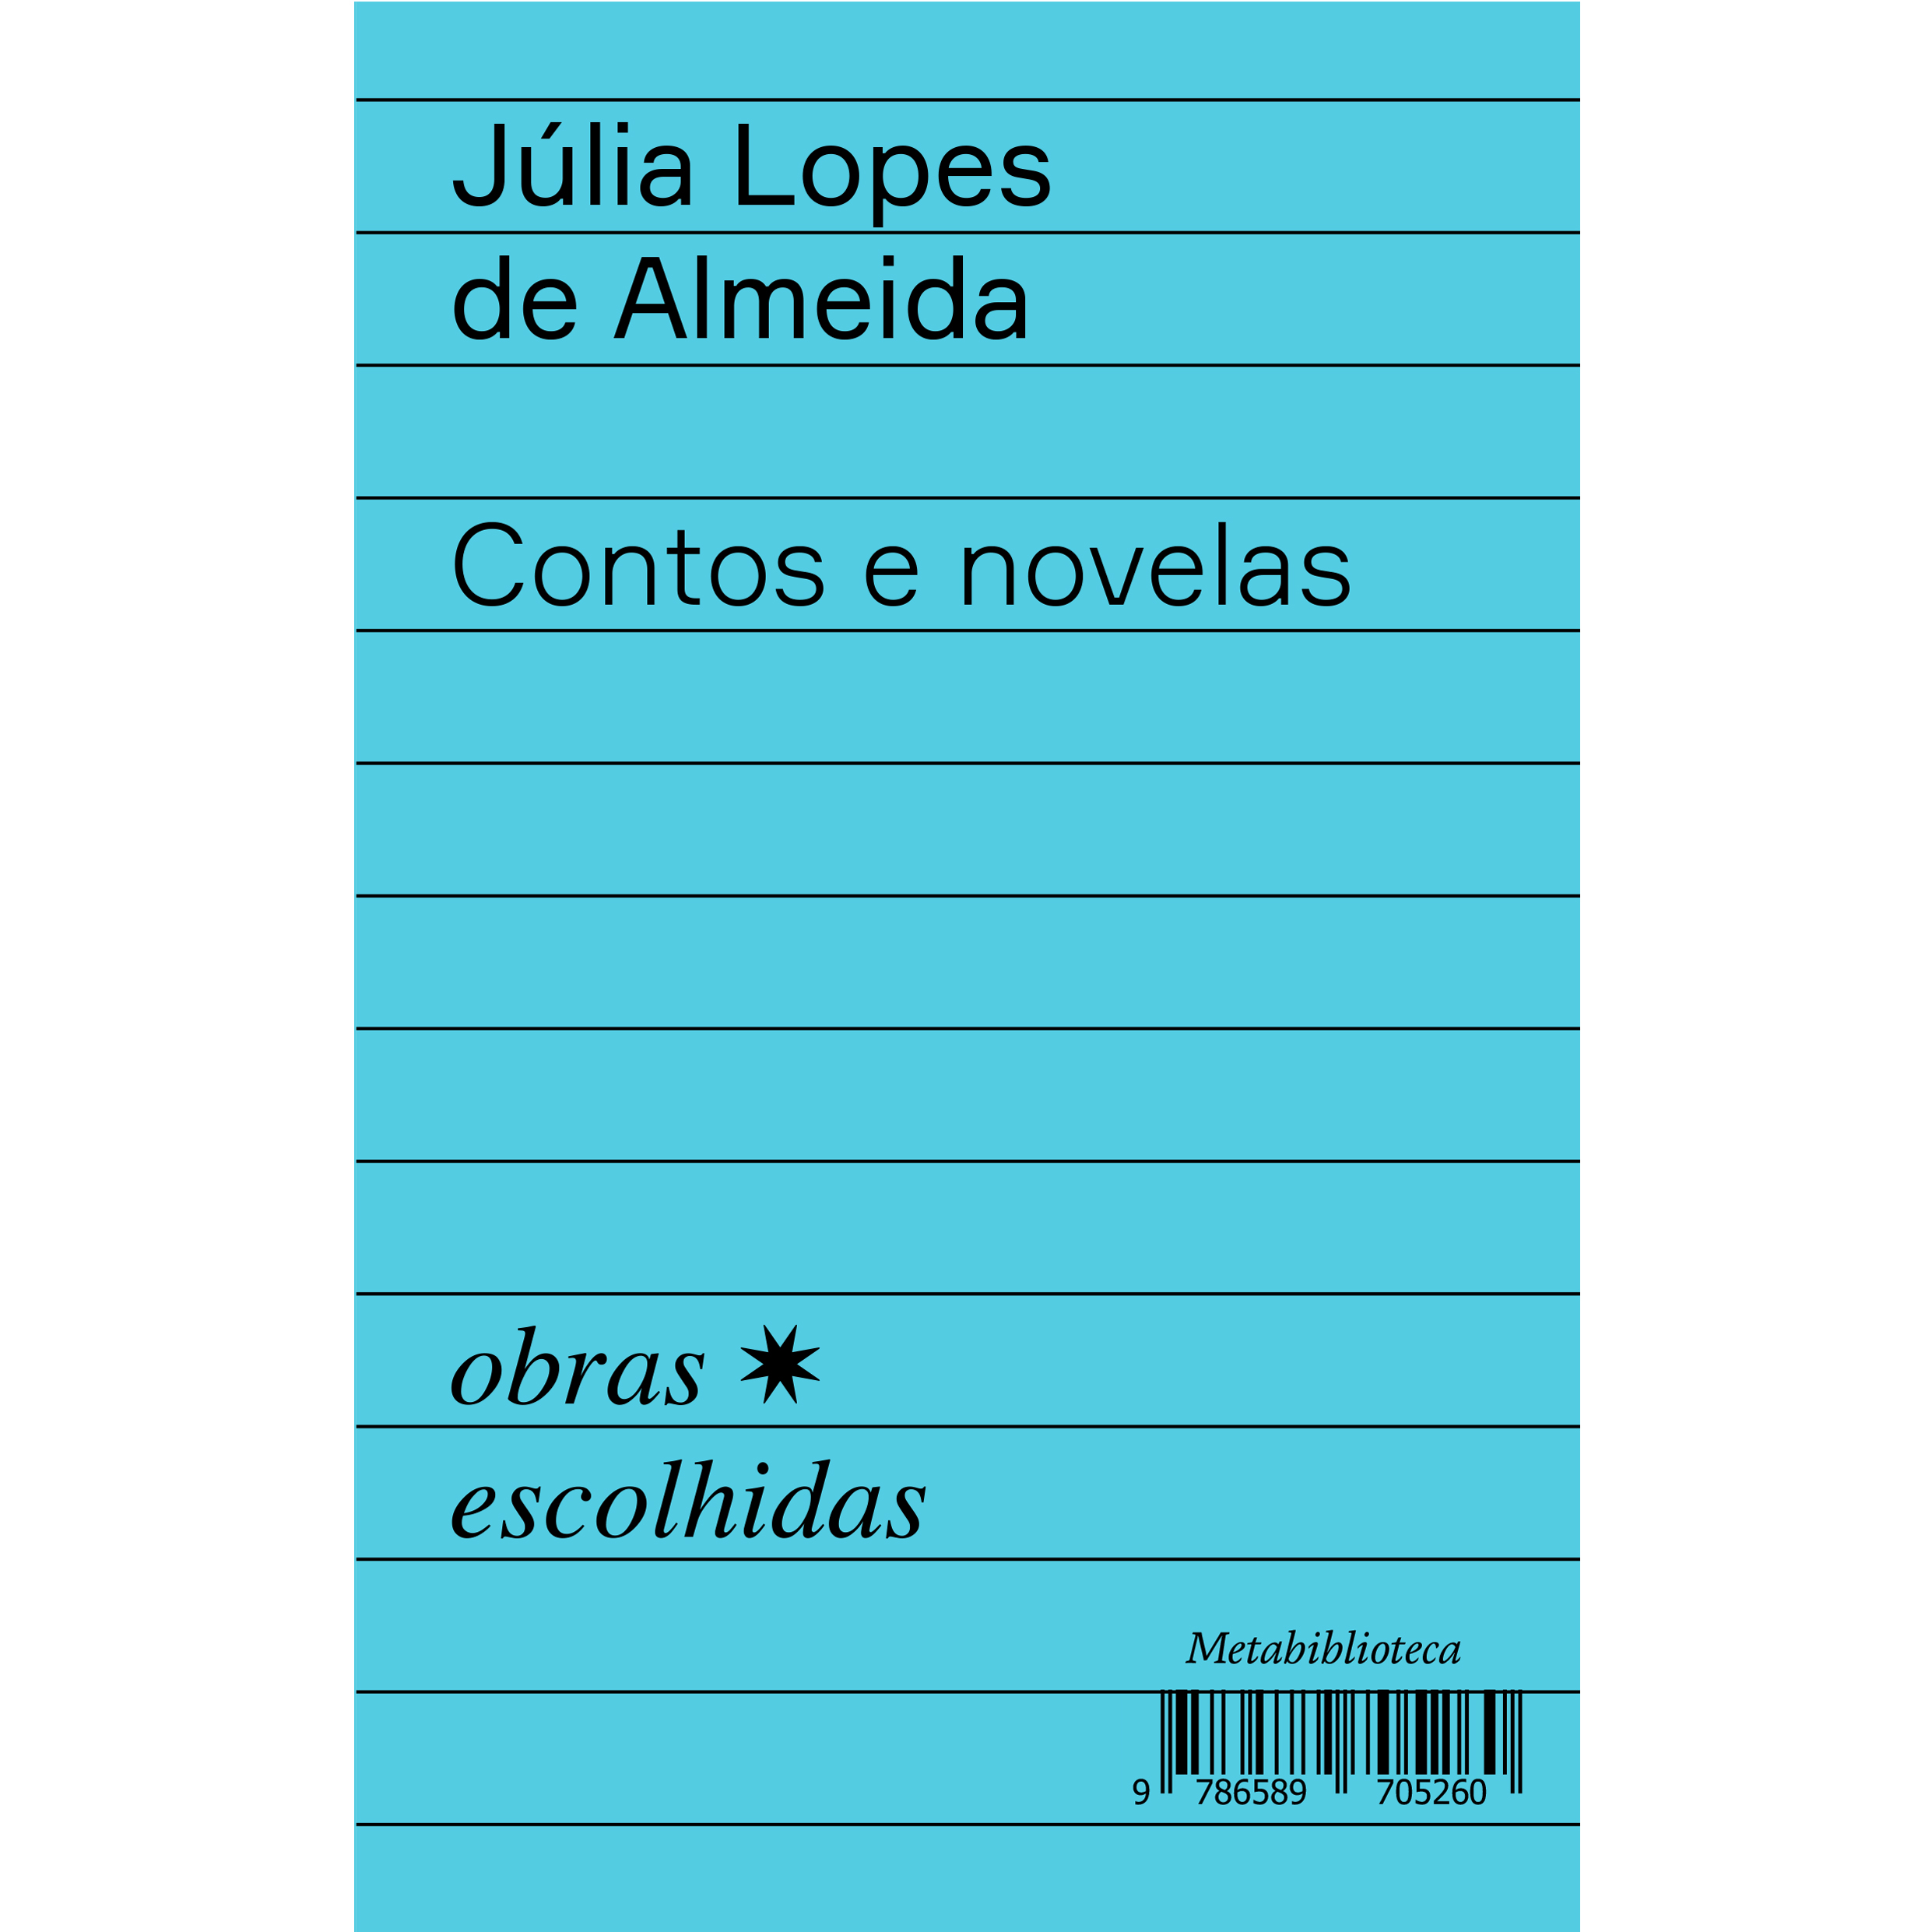
\includegraphics[width=74mm]{./CAPAS/HEDRA_JULIA.jpg}
\end{center}
\hspace*{-7cm}\hrulefill\hspace*{-7cm}
\medskip

\noindent{}\textit{Contos e novelas} reúne narrativas curtas de Júlia Lopes de Almeida, extraídas de duas de suas obras: \textit{Ânsia eterna} (1903) e \textit{A isca} (1922). Da primeira, fortemente influenciada pelo escritor francês Guy de Maupassant, foram selecionados dez contos, marcados pelo insólito e pelo fantástico. Da segunda, que reunia originalmente quatro novelas, foram selecionadas duas que apresentam algumas das características da narrativa de Júlia Lopes e dos temas que permeiam sua obra. Com tintas do naturalismo e do realismo francês, sua prosa tem traços da objetividade, do antropocentrismo e do cientificismo que fizeram escola no século XIX. \hlc{Não ficam de fora, no entanto, as críticas à sociedade brasileira: o lugar da mulher na sociedade patriarcal, os conflitos familiares, as marcas da escravidão e os contrastes sociais, políticos e econômicos} resultantes da modernização são temas recorrentes.

\vfill
\noindent\begin{minipage}[c]{1\linewidth}
{\small\textbf{
\hspace*{-.1cm}Editora: Hedra\\
Título: Contos e novelas: obras escolhidas\\
Autor: Júlia Lopes de Almeida\\ 
ISBN: 978-65-89705-26-0\\
Páginas: 190\\
Formato: 13,3x21\,cm\\
Preço: R\$ 64,00\\
}}
\end{minipage}
\pagebreak

\begin{center}
\hspace*{.5cm}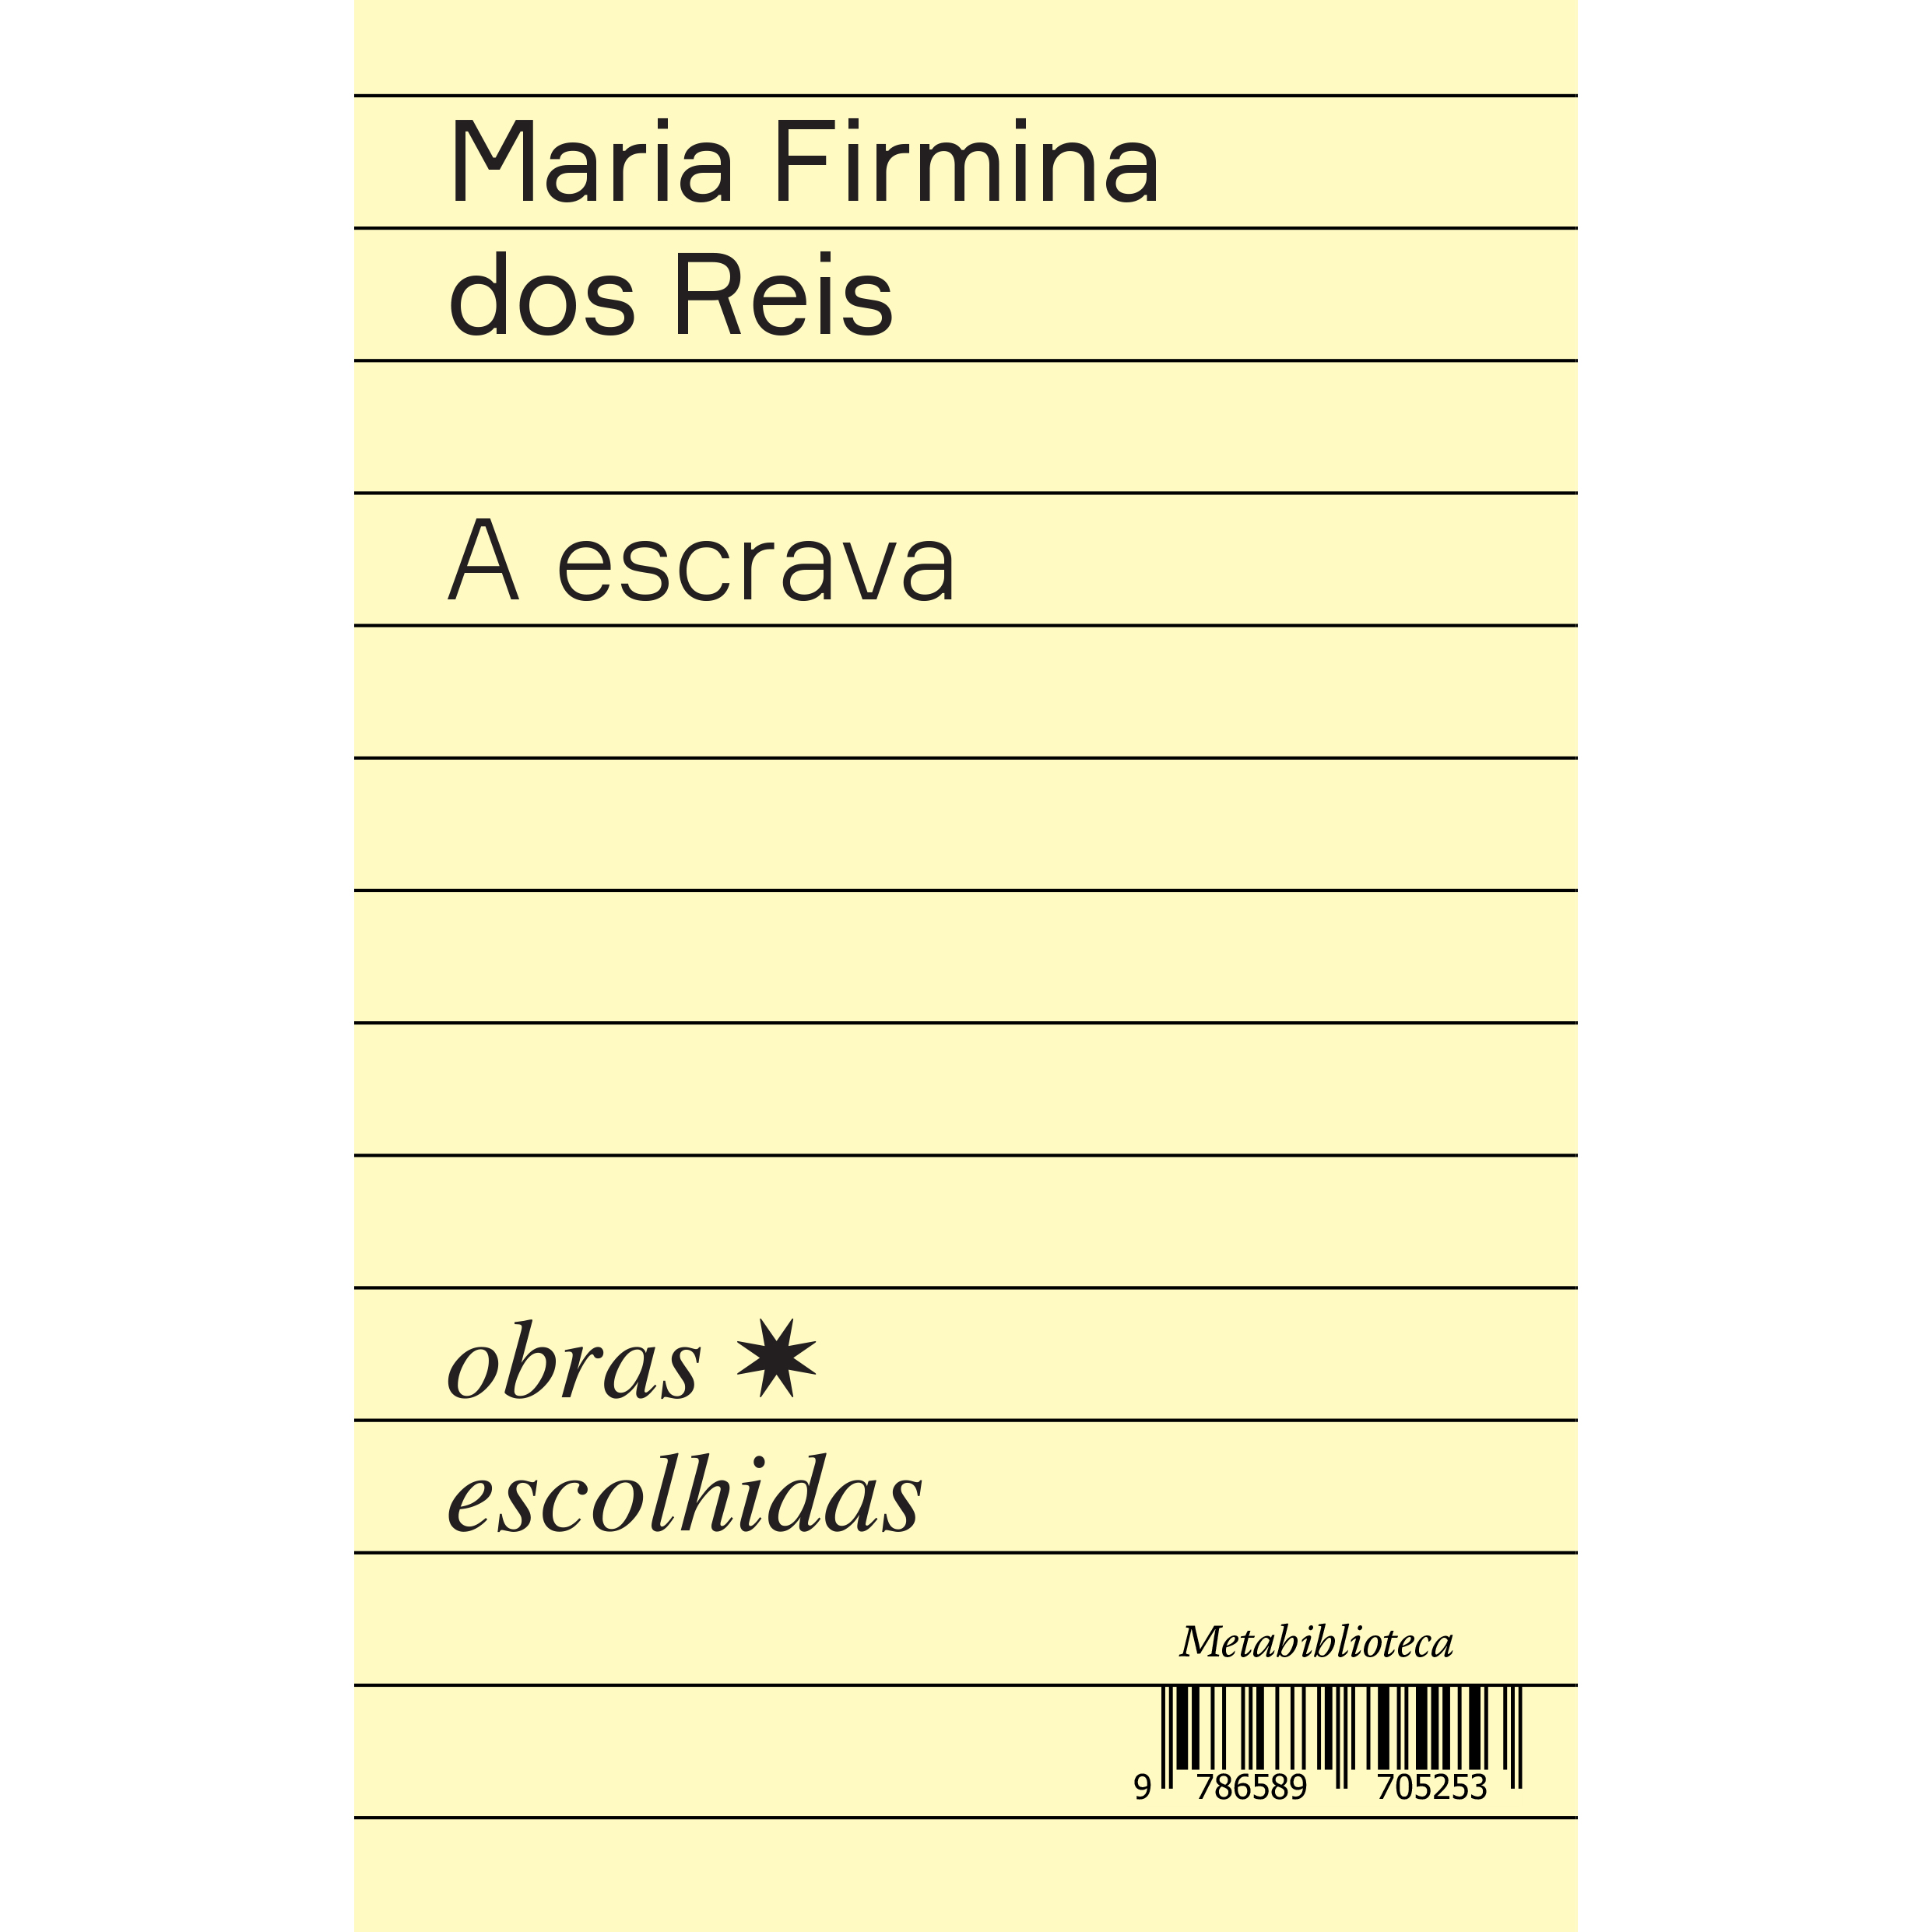
\includegraphics[width=74mm]{./CAPAS/HEDRA_FIRMINA.jpg}
\end{center}
\hspace*{-7cm}\hrulefill\hspace*{-7cm}
\medskip

\noindent{}\textit{A escrava} consiste em uma seleção de textos em prosa e poemas de Maria Firmina dos Reis (1822–1917), considerada a primeira romancista negra da história da literatura brasileira. Estão presentes o conto ``A escrava'', de 1887, a novela ``Gupeva'', de 1861, e 32 poemas: dos quais 29 foram extraídos entre os 56 de \textit{Cantos à beira-mar} (1871), dois da antologia \textit{Parnaso maranhense} (1861), e o famoso ``Hino à liberdade dos escravos'', originalmente escrito para ser cantado e acompanhado por instrumentos musicais. Nesta seleção, apresentam-se alguns dos principais elementos que caracterizam a literatura da escritora: \hlc{a situação dos escravizados, que passam a ter protagonismo nas narrativas, o papel da mulher na sociedade, as condições dos povos indígenas, um sentimentalismo romântico amoroso e a exaltação da terra.}

\vfill
\noindent\begin{minipage}[c]{1\linewidth}
{\small\textbf{
\hspace*{-.1cm}Editora: Hedra\\
Título: A escrava: antologia de prosa e versos\\
Autor: Maria Firmina dos Reis\\ 
ISBN: 978-65-89705-25-3\\
Páginas: 162\\
Formato: 13,3x21\,cm\\
Preço: R\$ 56,00\\
}}
\end{minipage}
\pagebreak

\begin{center}
\hspace*{-3.6cm}\raisebox{5cm}{\rotatebox[origin=t]{90}{\huge\textbf{Lançamento}}}
\hspace*{3.1cm}
\includegraphics[width=74mm]{./CAPAS/HEDRA_ARUAQUES.jpg}
\end{center}
\hspace*{-7cm}\hrulefill\hspace*{-7cm}
\medskip

\noindent{}\textit{Os aruaques} é um \hlc{livro clássico, escrito antes da Primeira Guerra Mundial, sobre os povos indígenas falantes de línguas aruaque. Durante suas expedições, Max Schmidt já tinha observado a influência cultural dos povos aruaques sobre outros grupos, o que estimulou interesse por sua enorme expansão geográfica} nas terras baixas da América do Sul: o problema central não seria descobrir a origem geográfica dos aruaques, mas explicar sua dinâmica cultural. 

Schmidt opera com distinções claras entre língua e cultura, e conceitos como \textit{aculturação}, \textit{difusão} e \textit{mudança cultural}. Seu argumento principal é que outros autores, anteriores a ele, não teriam levantado as questões certas sobre sua expansão, por isso a falta de respostas satisfatórias. Sua teoria de fato é diferente dos antecessores, mostrando grande originalidade para a época. \textit{Die Aruaken} é a segunda tese de doutorado de Max Schmidt (1874--1950), que já tinha realizado três expedições na América do Sul, em 1900--01, 1910 e 1914.

\vfill
\noindent\begin{minipage}[c]{1\linewidth}
{\small\textbf{
\hspace*{-.1cm}Editora: Hedra\\
Título: Os Aruaques\\
Autor: Max Schmidt\\ 
ISBN: 978-65-89705-22-2\\
Páginas: 182\\
Formato: 13,3x21\,cm\\
Preço: R\$ 57,00\\
}}
\end{minipage}
\pagebreak

\begin{center}
\hspace*{.5cm}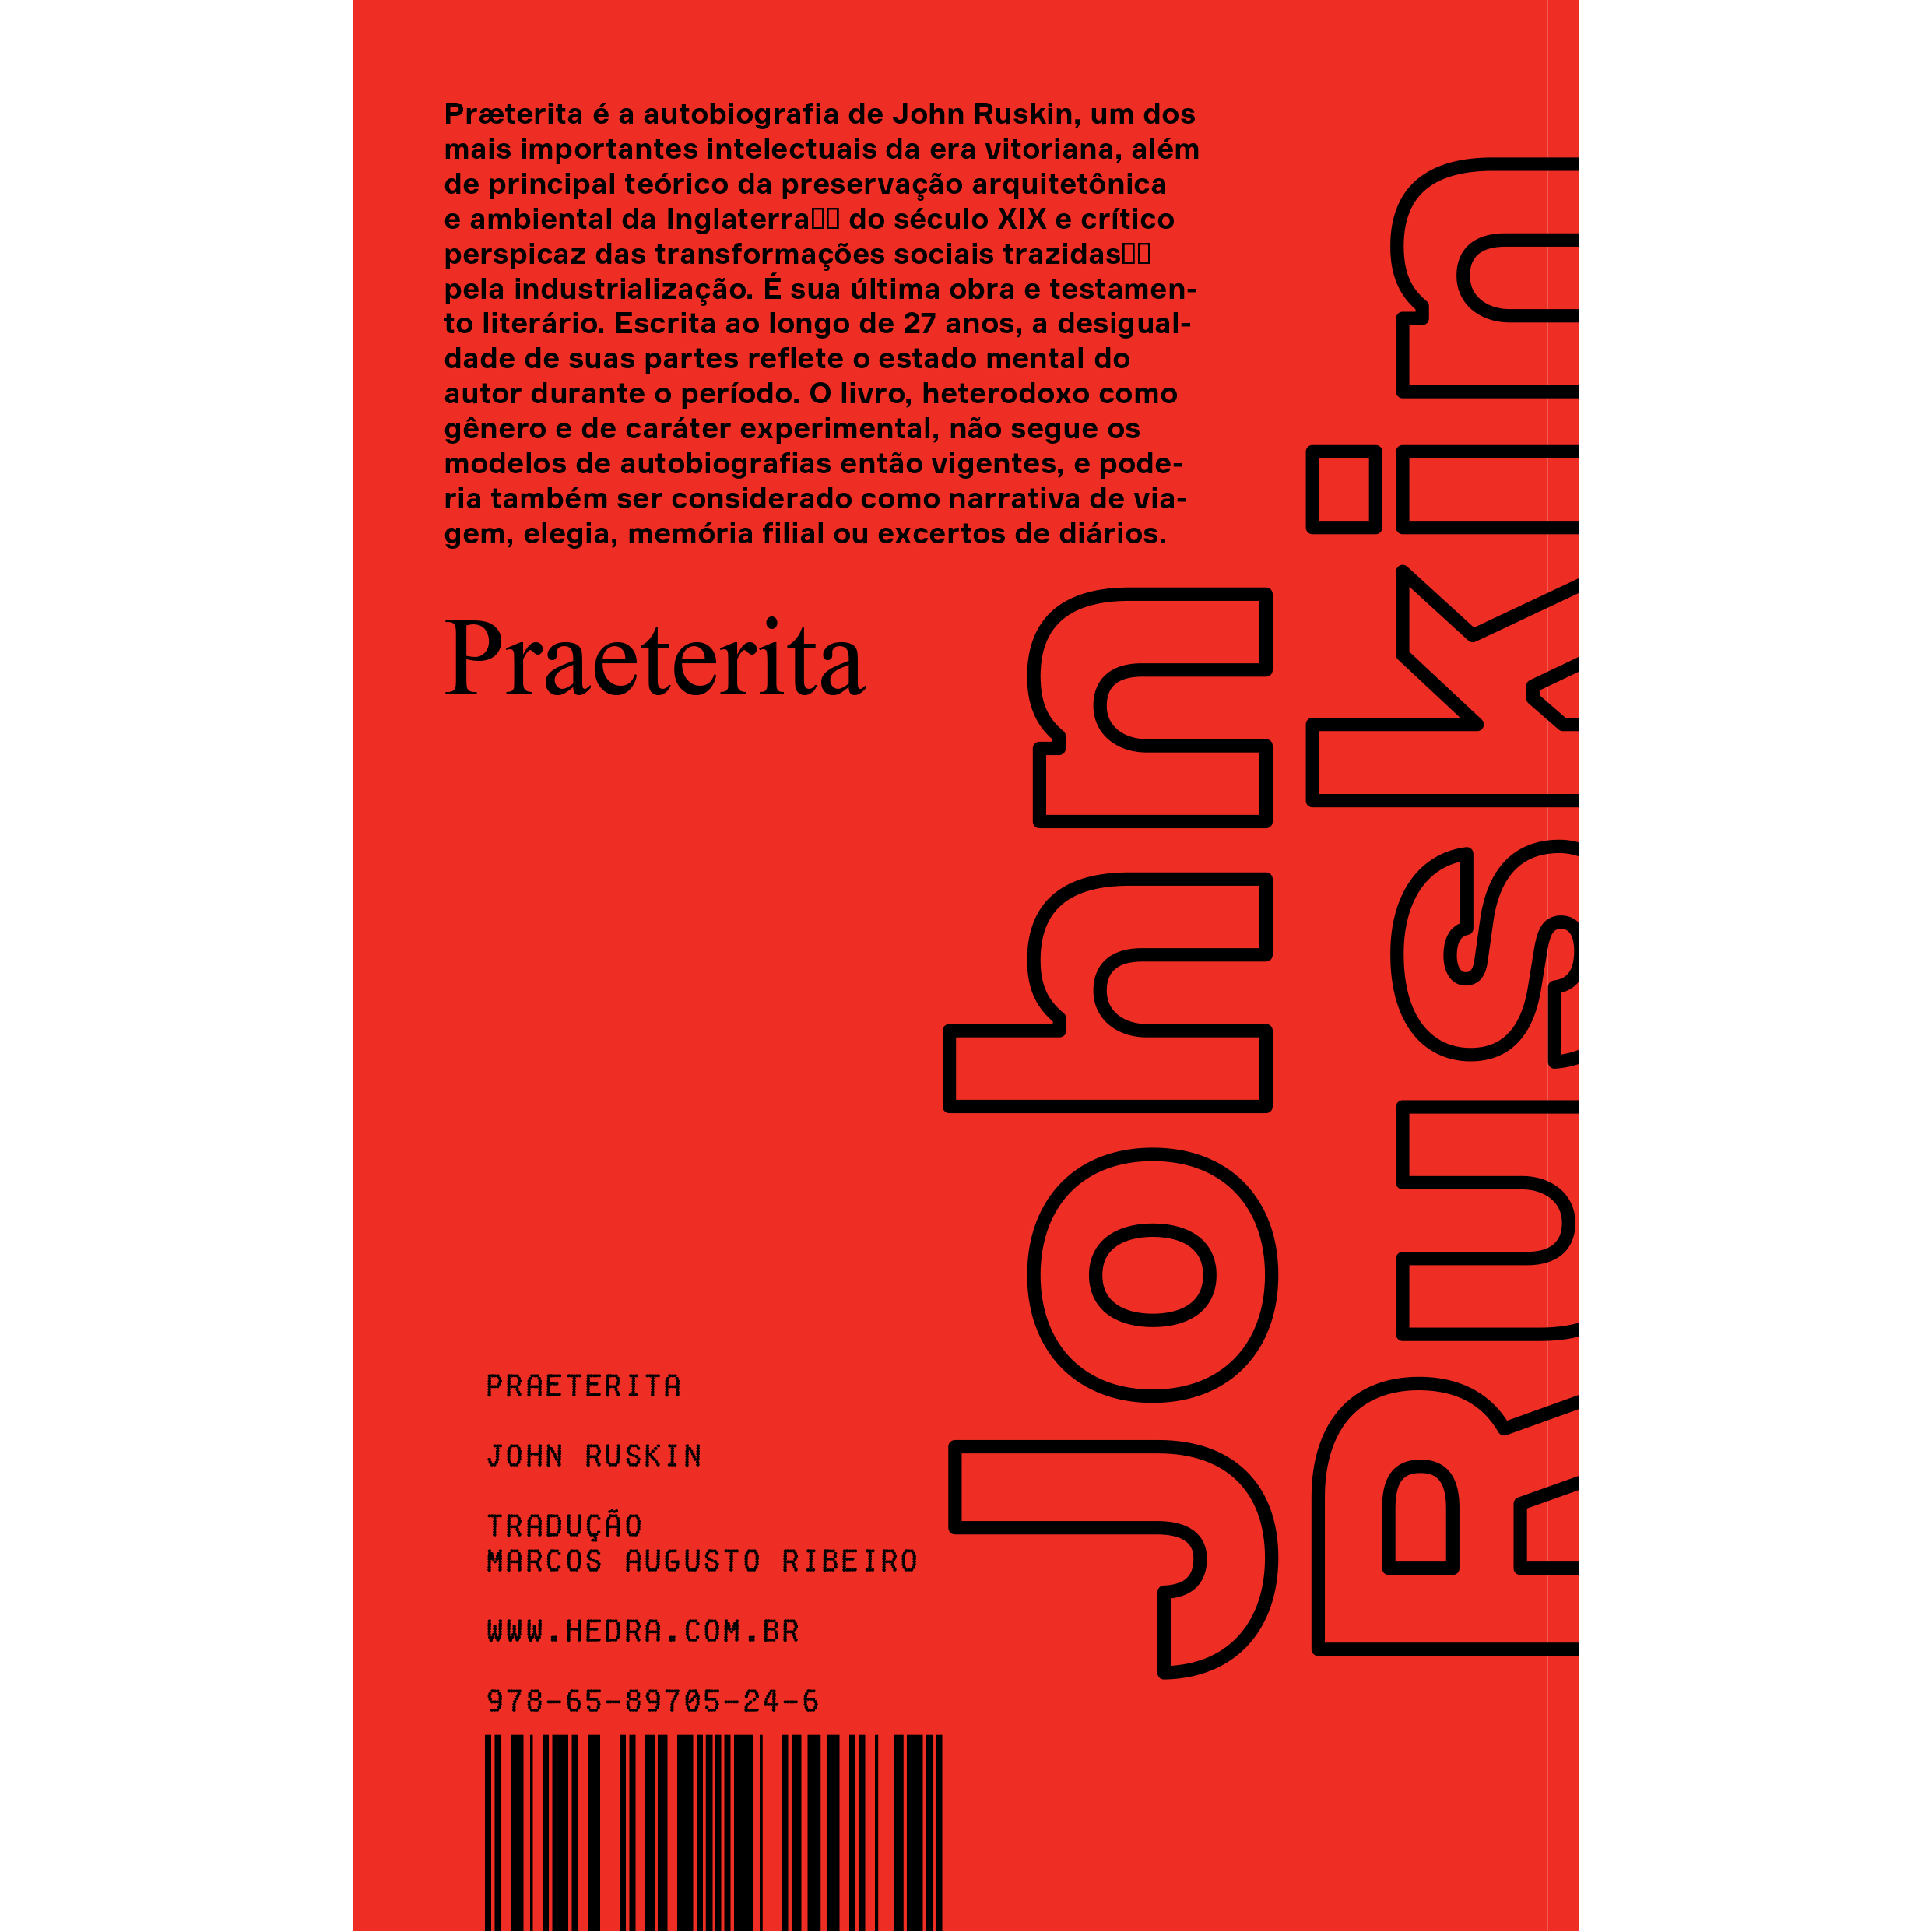
\includegraphics[width=74mm]{./CAPAS/HEDRA_RUSKIN.jpg}
\end{center}
\hspace*{-7cm}\hrulefill\hspace*{-7cm}
\medskip

\noindent{}John Ruskin (1819--1900), \hlc{foi um dos mais importantes intelectuais da era vitoriana. Principal teórico da preservação arquitetônica e ambiental da Inglaterra do século XIX e crítico perspicaz das transformações sociais trazidas ao país pela industrialização}, a qual veementemente combateu. Excêntrico, vinculado ao romantismo, grande esteta, valorizava a sensibilidade subjetiva em contraponto à razão; contraditório --- ao mesmo tempo aristocrático, reacionário e simpático ao socialismo. \textit{Prætērita}, sua autobiografia, foi sua última obra e testamento literário. Escrita ao longo de 27 anos, a desigualdade de suas partes reflete o estado mental do autor durante o período de sua elaboração. O livro, heterodoxo como gênero e de caráter ``experimental'', não segue os modelos de autobiografias então vigentes --- geralmente apresentados em termos de confissão religiosa ---, e poderia também ser considerado como narrativa de viagem, elegia, memória filial ou coleção de excertos de diários. Esta tradução contempla apenas o primeiro dos três volumes de \textit{Prætērita}.

\vfill
\noindent\begin{minipage}[c]{1\linewidth}
{\small\textbf{
\hspace*{-.1cm}Editora: Hedra\\
Título: Prætērita\\
Autor: John Ruskin\\ 
ISBN: 978-65-89705-24-6\\
Páginas: 246\\
Formato: 13,3x21\,cm\\
Preço: R\$ 66,00\\
}}
\end{minipage}
\pagebreak

\begin{center}
\hspace*{-3.6cm}\raisebox{5cm}{\rotatebox[origin=t]{90}{\huge\textbf{Lançamento}}}
\hspace*{3.1cm}\includegraphics[width=74mm]{./CAPAS/HEDRA_SOCIEDADE.jpg}
\end{center}
\hspace*{-7cm}\hrulefill\hspace*{-7cm}
\medskip

\noindent{}As relações sociais passaram a figurar cada vez mais em ambientes digitais, e se transformaram em elementos de controle e disputas. É o \hlc{chamado \textit{capitalismo informacional}, baseado na coleta, monitoramento e análise de dados pessoais. Se deveriam circular livremente em redes distribuídas globalmente, têm sido coletados constantemente e utilizados sem que saibamos como e por quê} e, em grande parte, fora de regulamentação. É neste cenário que as corporações têm se apropriado da tecnologia para se colocar à frente da concorrência, ao passo que governos as usam como dispositivos de controle sobre os cidadãos. Para compreender esse fenômeno, pesquisadores se propõem a analisar neste livro as tensões da sociedade de controle, se apoiando nas contribuições de Gilbert Simondon, Félix Guattari, Gilles Deleuze, Maurizio Lazzarato, Michel Foucault, Manuel Castells, Frank Pasquale, Shoshana Zuboff, entre outros.

\vfill
\noindent\begin{minipage}[c]{1\linewidth}
{\small\textbf{
\hspace*{-.1cm}Editora: Hedra\\
Título: A sociedade de controle: manipulação e\\modulação nas redes digitais\\
Autor: Joyce Souza, Rodolfo Avelino e\\Sérgio Amadeu da Silveira (orgs.)\\ 
ISBN: 978-65-89705-19-2\\
Páginas: 160\\
Formato: 12,7x19,1\,cm\\
Preço: R\$ 59,00\\
}}
\end{minipage}
\pagebreak

\begin{center}
\hspace*{.5cm}\includegraphics[width=74mm]{./CAPAS/HEDRA_ATIVISMO.jpg}
\end{center}
\hspace*{-7cm}\hrulefill\hspace*{-7cm}
\medskip

\noindent{}\textit{Ativismo digital hoje} reúne nove textos que refletem, de diferentes óticas, sobre a influência das redes sociais na política e na cultura atualmente: \hlc{ciberfeminismo, democracia digital, políticas online, ativismo online, cibervigilância, conflitos nas redes sociais, governo aberto, governança da Internet e cultura digital} são alguns dos temas explorados.
Pela abrangência do assunto, os artigos são divididos em três eixos: ciberpolítica, com enfoque na interface digital da política; ciberativismo, que percorre as alterações no campo do ativismo ocorridas desde a década de 1990; e cibercultura, que explora a emergência de práticas culturais e a expressão de subjetividades em consonância com as novas práticas comunicacionais do meio digital.

\vfill
\noindent\begin{minipage}[c]{1\linewidth}
{\small\textbf{
\hspace*{-.1cm}Editora: Hedra\\
Título: Ativismo digital hoje: política e\\cultura na era das redes\\
Autor: Rosemary Segurado, Claudio Penteado e\\Sérgio Amadeu da Silveira (orgs.)\\ 
ISBN: 978-85-7715-616-0\\
Páginas: 238\\
Formato: 12,7x19,1\,cm\\
Preço: R\$ 74,00\\
}}
\end{minipage}
\pagebreak

\begin{center}
\hspace*{-3.6cm}\raisebox{5cm}{\rotatebox[origin=t]{90}{\huge\textbf{Lançamento}}}
\hspace*{3.1cm}\includegraphics[width=74mm]{./CAPAS/HEDRA_CAMARA.jpg}
\end{center}
\hspace*{-7cm}\hrulefill\hspace*{-7cm}
\medskip

\noindent{}Aguardando descrição.

\vfill
\noindent\begin{minipage}[c]{1\linewidth}
{\small\textbf{
\hspace*{-.1cm}Editora: Hedra\\
Título: Câmara escuro\\
Autor: Moacir Amâncio\\ 
ISBN: 978-65-89705-27-7\\
Páginas: 73 (provisório)\\
Formato: 13,3x21\,cm\\
Preço: R\$ 34,00 (provisório)\\
}}
\end{minipage}
\pagebreak

\begin{center}
\hspace*{.5cm}\includegraphics[width=74mm]{./CAPAS/HEDRA_GOLDMAN.jpg}
\end{center}
\hspace*{-7cm}\hrulefill\hspace*{-7cm}
\medskip

\noindent{}Sob perspectiva da implacável anarquista que foi Emma Goldman, \textit{Sobre anarquismo, sexo e casamento} trata de temas como o \hlc{controle de natalidade, o puritanismo norte-americano, a repressão sexual, o amor livre, o ciúme, a prostituição, a homossexualidade, a desigualdade entre os sexos, a maternidade, a emancipação feminina, o movimento sufragista na Inglaterra e Estados Unidos e a trajetória de uma série de mulheres extraordinárias}, dentre elas heroínas e mártires do movimento revolucionário russo. 

O contexto no qual esses textos foram escritos passou pela Primeira Guerra Mundial, a Revolução Russa e a ascensão do fascismo italiano e do nacional-socialismo na Alemanha. Dada a sua condição de russa, judia, anarquista e crítica implacável do puritanismo estadunidense à autocracia soviética, tornavam-lhe ainda mais vulnerável --- dos Estados Unidos à Rússia, e nos mais diferentes círculos.

\vfill
\noindent\begin{minipage}[c]{.5\linewidth}
{\small\textbf{
\hspace*{-.1cm}Editora: Hedra\\
Título: Sobre anarquismo,\\sexo e casamento\\
Autor: Emma Goldman\\ 
ISBN: 978-65-89705-23-9\\
Páginas: 264 (provisório)\\
Formato: 13,3x21\,cm\\
Preço: R\$ 69,90 (provisório)\\
}}
\end{minipage}
\pagebreak

\begin{center}
\hspace*{-3.6cm}\raisebox{5cm}{\rotatebox[origin=t]{90}{\huge\textbf{Lançamento}}}
\hspace*{3.1cm}\includegraphics[width=74mm]{./CAPAS/BREVE.jpg}
\end{center}
\hspace*{-7cm}\hrulefill\hspace*{-7cm}
\medskip

\noindent{}As plataformas digitais foram fundamentais para diminuir o impacto do distanciamento social durante a pandemia da Covid-19. A internet e as redes sociais digitais passaram a ser a janela para o mundo para muitos e através dela eram realizadas atividades profissionais, encontros entre amigos e familiares, compras e vendas online, aulas, consultas médicas e acesso à cultura. 

\hlc{A vida estava, enfim, circunscrita às telas de nossos computadores e celulares, embora a maior parte da população brasileira não pudesse se manter em isolamento social. Mas foi também por meio delas verificamos o aumento do compartilhamento de informações falsas}, mentiras e boatos sobre a pandemia. O Brasil ocupou o triste lugar de país que mais compartilha informações falsas ou duvidosas sobre o coronavírus.

\vfill
\noindent\begin{minipage}[c]{1\linewidth}
{\small\textbf{
\hspace*{-.1cm}Editora: Hedra\\
Título: Democracia e desinformação: fake news na internet\\
Autor: Rosemary Segurado (org.)\\ 
ISBN: 978-65-89705-34-5\\
Páginas: 238 (provisório)\\
Formato: 12,7x19,1\,cm\\
Preço: R\$ 74,00 (provisório)\\
}}
\end{minipage}
\pagebreak

\begin{center}
\hspace*{.5cm}\includegraphics[width=74mm]{./CAPAS/HEDRA_ROBINSON.jpg}
\end{center}
\hspace*{-7cm}\hrulefill\hspace*{-7cm}
\medskip

\noindent{}Daniel Defoe (1660--1731) escreveu \textit{Robinson Crusoé} em primeira pessoa, livro que segue o modo epistolar de um diário. Publicado durante uma época conhecida por fazer ascender o romance, seus detalhes objetivos influenciaram Herman Melville, em \textit{Moby Dick} (1851).

O náufrago Robinson Crusoé, que dá nome ao livro, \hlc{é uma espécie de autobiografia fictícia de um homem que passou 28 anos em uma remota ilha tropical encontrando canibais cativos e revoltosos antes de ser resgatado}. Originalmente publicado na forma de folhetins no \textit{The Daily Post}, é um clássico lido em diversas versões --- até mesmo em adaptações infanto-juvenis. É, todavia, uma obra complexa e seus contornos históricos até hoje propõem discussões. 

\vfill
\noindent\begin{minipage}[c]{1\linewidth}
{\small\textbf{
\hspace*{-.1cm}Editora: Hedra\\
Título: Robinson Crusoé\\
Autor: Daniel Defoe\\ 
ISBN: 978-65-89705-31-4\\
Páginas: 350 (provisório)\\
Formato: 13,3x21\,cm\\
Preço: R\$ 89,00 (provisório)\\
}}
\end{minipage}
\pagebreak

\begin{center}
\hspace*{-3.6cm}\raisebox{5cm}{\rotatebox[origin=t]{90}{\huge\textbf{Lançamento}}}
\hspace*{3.1cm}\includegraphics[width=74mm]{./CAPAS/HEDRA_CANTOS.jpg}
\end{center}
\hspace*{-7cm}\hrulefill\hspace*{-7cm}
\medskip

\noindent{}Neste livro são apresentadas \hlc{26 histórias de aves e outros animais da mata, acompanhados pelos cantos \textit{guahu} que cantam sua história desde o princípio dos tempos.} Esses \textit{guahu} fazem parte de um conjunto maior de cantos, rezas e danças dominados por Atanásio Teixeira ou Ava Ñomoandyja, um dos mais prestigiosos xamãs do povo Guarani Kaiowá. As narrativas e explicações que acompanham os cantos foram elaboradas pelo historiador Izaque João, a partir de falas e orientações de Atanásio Teixeira ao longo dos últimos seis anos. 

Os processos de seleção, transcrição e tradução para esta edição bilíngue também foram feitos em diálogo com o xamã e as versões em português dos textos e cantos \textit{guahu} são um exercício de aproximação de suas belas palavras.

\vfill
\noindent\begin{minipage}[c]{1\linewidth}
{\small\textbf{
\hspace*{-.1cm}Editora: Hedra\\
Título: Cantos dos animais primordiais\\
Autor: Ava Ñomoandyja Atanásio Teixeira\\ 
ISBN: 978-65-89705-30-7\\
Páginas: 200 (provisório)\\
Formato: 13,3x21\,cm\\
Preço: R\$ 69,00 (provisório)\\
}}
\end{minipage}
\pagebreak

% \begin{center}
% \hspace*{.5cm}\includegraphics[width=74mm]{./CAPAS/HEDRA_CRIME.jpg}
% \end{center}
% \hspace*{-7cm}\hrulefill\hspace*{-7cm}
% \medskip

% \noindent{}\textit{Crime} apresenta \hlc{a volta de Luiz Gama ao direito a partir de textos que são, em sua maioria, casos criminais: petições de \textit{habeas corpus}, denúncias de violação de direitos de presos e prisões ilegais.} E tornam este livro uma espécie de desenvolvimento do quinto volume, \textit{Direito}. Relacionados à matéria penal e processual penal, \textit{Crime} revela o conhecimento de causa com que interpretava o direito criminal do Brasil. Uma habilidade técnica que outros --- que o chamavam \textit{rábula} --- tentam diminuir, ocultar ou desprezar.

% \textit{Crime} integra as \textit{Obras completas} de Luiz Gama, advogado negro e abolicionista, a serem lançadas em 11 volumes com cerca de 800 escritos --- 600 inéditos ---, revelando as diversas facetas e estilos empregados pelo escritor para advogar pela grande causa de sua vida: a abolição da escravidão e a emancipação negra. Esquecidos em parte por quase dois séculos, os textos foram recuperados pelo pesquisador Bruno Rodrigues de Lima, que passou nove anos localizando-os em arquivos da imprensa e do judiciário de todo o país.

% \vfill
% \noindent\begin{minipage}[c]{1\linewidth}
% {\small\textbf{
% \hspace*{-.1cm}Editora: Hedra\\
% Título: Crime [1877--1879]\\
% Autor: Luiz Gama\\ 
% ISBN: 978-65-89705-15-4\\
% Páginas: Inserir.\\
% Formato: 13,3x21\,cm\\
% Preço: R\$ Inserir.\\
% }}
% \end{minipage}
% \pagebreak

% \begin{center}
% \hspace*{.5cm}\includegraphics[width=74mm]{./CAPAS/HEDRA_DIREITO.jpg}
% \end{center}
% \hspace*{-7cm}\hrulefill\hspace*{-7cm}
% \medskip

% \noindent{}\textit{Direito} é marcado pela saída de Luiz Gama da polícia e o início de seu percurso como advogado. Este volume reúne sua literatura normativo-pragmática: são textos que podem ser lidos segundo divisões temáticas internas do direito e a partir dos casos concretos. \hlc{A maioria dos textos trata de causas que envolvem escravidão e liberdade, mas Gama também atuou em causas de outras naturezas jurídicas}, eminentemente técnicas, sem lidar com a questão da vida e da morte, o que revela o domínio intelectual do advogado.

% \textit{Direito} integra as \textit{Obras completas} de Luiz Gama, advogado negro e abolicionista, a serem lançadas em 11 volumes com cerca de 800 escritos --- 600 inéditos ---, revelando as diversas facetas e estilos empregados pelo escritor para advogar pela grande causa de sua vida: a abolição da escravidão e a emancipação negra. Esquecidos em parte por quase dois séculos, os textos foram recuperados pelo pesquisador Bruno Rodrigues de Lima, que passou nove anos localizando-os em arquivos da imprensa e do judiciário de todo o país.

% \vfill
% \noindent\begin{minipage}[c]{1\linewidth}
% {\small\textbf{
% \hspace*{-.1cm}Editora: Hedra\\
% Título: Direito [1870--1875]\\
% Autor: Luiz Gama\\ 
% ISBN: 978-65-89705-13-0\\
% Páginas: 400 (provisório)\\
% Formato: 13,3x21\,cm\\
% Preço: R\$ 90,00 (provisório)\\
% }}
% \end{minipage}
% \pagebreak

\vspace*{1.5cm}
\noindent{}{\nohyphens{\LARGE{Um novo patamar da luta\\política abolicionista}}}
\bigskip

\hfill{}\scalebox{.8}{BRUNO RODRIGUES DE LIMA}
\bigskip
\bigskip
\bigskip

\begin{multicols}{2}
\noindent{}Como Luiz Gama radicalizou a luta abolicionista no Brasil? Quais foram suas táticas de luta --- no debate, na imprensa e nos tribunais? Quem esteve ao seu lado a toda 
hora --- e quem atravessou a rua de fininho e mudou de calçada?
O volume \textit{Liberdade} reúne textos que respondem a essas, e outras, perguntas.

Partindo do início de 1880 e chegando até a morte de Gama, em agosto de 1882, \textit{Liberdade} sintetiza a visão política da maior liderança abolicionista de São Paulo na última década da escravidão no Brasil. Jornalista e advogado experiente, Gama usaria de sua veia literária para mudar a chave narrativa e operar uma clivagem conceitual e prática no reposicionamento do movimento abolicionista em São Paulo, que viria a ter repercussão em todo o país. Muito de caso pensado, Gama politizará a racialização da violência e do terrorismo de Estado, radicalizando, assim, o discurso abolicionista a níveis nunca antes vistos. E o fará na esfera discursiva, em momentos decisivos, através de pseudônimos, convertidos em arma retórica e nexo de inflexão radicalizadora do conceito e da prática.

De modo inédito no abolicionismo brasileiro, Gama definiria a política da escravidão como significante indissociável de violência, crueldade, terror, crime e impunidade, ao passo em que enalteceria a resistência dos escravizados pardos e negros como ação política imbuída de indiscutível valor moral e autonomia da vontade.

\vspace{\baselineskip}
{\small\fakereceipt{
\noindent{}Quem abrisse os jornais daquela quarta"-feira, 1º de dezembro de 1880, principalmente no Rio de Janeiro ou em São Paulo, veria que três grandes polêmicas sobre a escravidão tomavam corpo na imprensa. Nas três, a presença do advogado negro Luiz Gama se destacava.
}}
\vspace{\baselineskip}

E Gama dirigia essa radicalização conceitual no abolicionismo com um sentido pragmático: conquistar a abolição e a cidadania ampla, geral e irrestrita o mais rápido possível. Para isso, posicionou o tema da violência racial e policial nos mais improváveis repertórios, como a filosofia do direito natural e o conhecimento normativo legislativo, doutrinário e jurisprudencial brasileiro, descrevendo em mínimos detalhes a estupidez branca e o terrorismo judiciário da política da escravidão.

Parte significativa dos próprios abolicionistas reagiria muito mal à mudança de chave narrativa de Gama. Joaquim Nabuco, por metonímia da classe, diria mais tarde que o seu abolicionismo era o de baluartes como Wilbeforce e Garrisson, e não o “de Spartacus, ou de John Brown”,\footnote{Joaquim Nabuco. \textit{O abolicionismo}. Londres: Tipografia de Abraham Kingdon, 1883, p.\,25.} aqui tomados como signos de fúria e barbárie.

Para bom entendedor, é claro que ele refutava oblíqua e dissimuladamente as ideias de Gama, que dois anos antes escrevera que desejava ser ``louco como Espártacos, como Lincoln, como John Brown, como Jesus''.\footnote{``A liberdade urge'', conforme cita o original.} Se ninguém serve a dois senhores, logo se verá que o abolicionismo de um não foi, e quiçá nunca mesmo poderia ter sido, o abolicionismo do outro.

Assim como o movimento que ele organizava, pode"-se dizer que Gama elegia ``retóricas, estratégias e arenas conforme a conjuntura política''.\footnote{Angela Alonso. \textit{Flores, votos e balas: o movimento abolicionista brasileiro (1868--88)}. São Paulo: Companhia das Letras, 2015, p.\,19.} No início da década de 1880, que lamentavelmente marcaria o final de sua vida, o advogado  mudava o patamar discursivo do abolicionismo no espaço público brasileiro, escolhendo a retórica da fúria negra, potencializada pelo uso de pseudônimos enquanto estratégia autoral, para disseminar sua voz por diferentes arenas de debates, sempre atento às injunções da conjuntura política --- sobretudo a da política local. A combinação explosiva desses elementos atordoaria correligionários, oponentes e inimigos. Mas inegavelmente representava a esperança de liberdade, justiça e cidadania para ``um milhão e quinhentas mil vítimas do mais abominável crime''.\footnote{``Terrorismo judiciário'', conforme cita o original.}

O Brasil de 1880 estava numa encruzilhada --- e Gama não tinha dúvida de que lado, e ao lado de quem estava.

Quem abrisse os jornais daquela quarta"-feira, 1º de dezembro de 1880, principalmente no Rio de Janeiro ou em São Paulo, veria que três grandes polêmicas sobre a escravidão tomavam corpo na imprensa. Nas três, a presença do advogado negro Luiz Gama se destacava. Na capa da \textit{Gazeta da Tarde}, folha carioca de viés abolicionista, aparecia o despretensioso ``trecho de uma carta'' que, como se confirmaria nos meses seguintes, seria a primeira das onze partes de uma das mais impressionantes, senão a mais radical obra política de Luiz Gama.\footnote{``Olho vivo no parlamento'', conforme cita o original.} 

Em São Paulo, onde conhecia a todos e era por todos conhecido, outros dois artigos ganharam as páginas naquele mesmo dia: um na \textit{Gazeta do Povo}, em que, defendendo o seu camarada José do Patrocínio, anunciava um novo patamar da luta política abolicionista;\footnote{``O meu companheiro José do Patrocinio'', conforme cita o original.} e outro artigo na \textit{Província de S.\,Paulo} onde, como se verá, teve de usar de um pseudônimo para denunciar a tortura e o assassinato de uma criança parda de sete anos de idade pelas mãos de dois senhores brancos, que a quiseram enterrar viva.\footnote{``Revirando as vísceras da medicina legal'', conforme cita o original.}

Os três artigos não foram, até hoje, lidos em conjunto. Trata"-se, portanto, de reunião inédita na literatura de Luiz Gama. Partes de uma mesma estratégia literária e editorial, os três artigos abrem portas para se compreender a obra do maior jurista da história desse país e a sua luta, com as roupas e as armas da imprensa e do direito, pela liberdade e pelos direitos dos humilhados, ofendidos e condenados da terra. Semelhantes no propósito, os três artigos, contudo, tinham formas e destinatários diferentes, o que explica terem sido publicados não em um, mas em três jornais distintos. Com isso, intensificava a presença abolicionista na imprensa, visando, certamente, acelerar o processo histórico em curso.

Na capital do Império, Gama era apresentado pela \textit{Gazeta da Tarde} como o maior líder abolicionista em São Paulo. Desse lugar, ele se dirigia ao público simpático às ideias que tinham em comum, mirando um movimento popular de massas que derrubasse a monarquia, que ele entendia ser a fonte de sustentação da escravidão. Suas cartas corriam no fio da navalha, entre a sobriedade do jurista erudito e a insurgência do revolucionário, emitindo múltiplas mensagens para a diversidade de atores na arena política, muito embora tivessem o objetivo prático de mobilizar os abolicionistas para um conjunto de ações em comum. Foi justamente nesse contexto, como reforço à construção de sua liderança junto ao movimento, agora em perspectiva nacional, que a \textit{Gazeta da Tarde} publicou seu perfil biográfico, destacando pela primeira vez a jornada épica do menino preto nascido livre, escravizado pelo próprio pai, que fugiu do cativeiro e conquistou sua liberdade para, no futuro, libertar mais de quinhentas pessoas ilegalmente escravizadas.

\bigskip
\noindent{}\textcolor{gray}{\footnotesize\slsc{\textls[-15]{Excerto da introdução do volume ``Liberdade'', oitavo volume das \textit{Obras completas} de Luiz Gama.}}}
\end{multicols}

\pagebreak
\pagestyle{hedracat}
\begin{multicols}{2}
\begin{enumerate}
\raggedright\nohyphens{
\item A sociedade de controle \textbf{Joyce Souza, Rodolfo Avelino, Sérgio Amadeu da Silveira}
\item O contador de histórias e outros textos \textbf{Walter Benjamin}
\item Diário parisiense e outros escritos \textbf{Walter Benjamin}
\item Rashômon e outros contos \textbf{Akutagawa}
\item A linguagem fascista \textbf{Carlos Piovezani, Emilio Gentile}
\item Teogonia \textbf{Hesíodo}
\item Liberdade (1880-1882) \textbf{Luiz Gama}
\item Poesia completa \textbf{Orides Fontela}
\item Sobre verdade e mentira \textbf{Friedrich Nietzsche}
\item A volta do parafuso \textbf{Henry James}
\item Democracia (1866-1869) \textbf{Luiz Gama}
\item Trabalhos e os dias \textbf{Hesíodo}
\item Deus e o Estado \textbf{Mikhail Bakunin}
\item Hino a Afrodite e outros poemas \textbf{Safo de Lesbos}
\item O princípio anarquista e outros ensaios \textbf{Piotr Alekseievitch Kropotkin}
\item Pandemia e anarquia \textbf{Edson Passetti, João da Mata, José Maria Carvalho Ferreira}
\item Lugar de negro, lugar de branco? \textbf{Douglas Rodrigues Barros}
\item O indivíduo, a sociedade e o Estado e outros ensaios \textbf{Emma Goldman}
\item Machismo, racismo, capitalismo identitário \textbf{Pablo Polese}
\item Dicionário de mitologia nórdica \textbf{Johnni Langer}
\item Freud e o patriarcado \textbf{Léa Silveira, Alessandra Martins Parente}
\item Dicionário de história e cultura da era Viking \textbf{Johnni Langer} 
\item O princípio do Estado e outros ensaios \textbf{Mikhail Bakunin}
\item Sobre a utilidade e a desvantagem da história para a vida \textbf{Friedrich Nietzsche}
\item Ode sobre a melancolia e outros poemas \textbf{John Keats}
\item O chamado de Cthulhu \textbf{H. P. Lovecraft}
\item Saga dos Volsungos \textbf{Anônimo}
\item Os sofrimentos do jovem Werther \textbf{Johann Wolfgang Von Goethe}
\item Memórias do subsolo \textbf{Fiódor Dostoiévski}
\item A monadologia e outros textos \textbf{Gottfried Leibniz}
}
\end{enumerate}
\end{multicols}

\pagebreak

\pagestyle{n-1}
\label{n-1}

\pagebreak


\begin{center}
\hspace*{.5cm}\includegraphics[width=74mm]{./CAPAS/N-1_HABITAT.jpg}
\end{center}

\hspace*{-7cm}\hrulefill\hspace*{-7cm}

\medskip

\noindent{}Neste ensaio visual, Paulo Tavares intervém em \textit{Habitat}, revista de artes e design editada pela arquiteta Lina Bo Bardi nos anos 1950. \hlc{Resignificando imagens e imaginários dominantes, \textit{Des-Habitat} nos carrega através de uma narrativa visual sobre a colonialidade da arquitetura moderna e suas mídias}, abrindo um horizonte para a potencial descolonização de seus legados. Com ensaio e design de Paulo Tavares, e prefácio da curadora Marion von Osten, em uma parceria entre agência autônoma e n-1 edições.

\vfill

\hspace*{-.4cm}\begin{minipage}[c]{1\linewidth}
\small\textbf{
\hspace*{-.1cm}Editora: n-1\\
Título: Des-Habitat\\
Autor: Paulo Tavares\\ 
ISBN: 978-65-86941-39-5\\
Páginas: 97\\
Formato: 23,5x33\,cm\\
Preço: R\$ 70,00\\
}
\end{minipage}

\pagebreak %PRAGMATISMO PULSIONAL


\begin{center}
\hspace*{-3.6cm}\raisebox{5cm}{\rotatebox[origin=t]{90}{\huge\textbf{Lançamento}}}
\hspace*{3.1cm}\includegraphics[width=74mm]{./CAPAS/N-1_JACQUES.jpg}
\end{center}

\hspace*{-7cm}\hrulefill\hspace*{-7cm}

\medskip

\noindent{}Não há tempo moderno, mas tempos modernos, \hlc{maneiras diferentes ou contraditórias de agenciar as temporalidades das artes do movimento}, suas continuidades, seus cortes, seus reajustes e suas retomadas, para produzir obras que respondam às condições do presente e às exigências do futuro.
\vfill

\hspace*{-.4cm}\begin{minipage}[c]{.8\linewidth}
\small\textbf{
\hspace*{-.1cm}Editora: n-1\\
Título: Tempos modernos: arte, tempo, política\\
Autor: Jacques Rancière\\ 
ISBN: 978-65-86941-40-1\\
Páginas: 160\\
Formato: 17x12\,cm\\
Preço: R\$ 65,00\\
}
\end{minipage}

\pagebreak

\begin{center}
\hspace*{.5cm}\includegraphics[width=74mm]{./CAPAS/N-1_POVO.jpg}
\end{center}

\hspace*{-7cm}\hrulefill\hspace*{-7cm}

\medskip

\noindent{}Este livro parte da análise de uma única situação, porém exemplar: um homem morre de morte injusta e violenta; mulheres se juntam para chorá-lo; logo mais é um povo em lágrimas que se reúne a elas. Ora, essa situação que se vê por toda parte foi esplendidamente retratada por Serguei Eisenstein em seu célebre filme \textit{O encouraçado Potemkin}. Mas como foi que Roland Barthes, uma das vozes mais influentes no domínio do discurso contemporâneo sobre as imagens, pôde considerar tal construção do \textit{pathos} ``vulgar'' e ``lamentável''?
A melhor resposta à crítica \textit{barthesiana} será fornecida pelo próprio Eisenstein na estrutura de sua sequência de imagens, assim como no discurso --- imenso, abundante, genial, tão importante quanto o dos maiores pensadores de seu tempo --- que ele sustenta sobre a questão das imagens patéticas. Descobre-se uma emoção que sabe dizer \textit{nós}, e não só \textit{eu}, um \textit{pathos} que não é apenas passivo, mas se constitui em \textit{práxis}: \hlc{quando as velhas carpideiras de Odessa, em volta do marinheiro morto, passam da lamentação à cólera, ``prestam queixa'' e exigem justiça, fazem nascer esse \textit{povo em armas} da revolução que vem.}

\vfill

\hspace*{-.4cm}\begin{minipage}[c]{.5\linewidth}
\small\textbf{
\hspace*{-.1cm}Editora: n-1\\
Título: Povo em lágrimas, povo em armas\\
Autor: Georges Didi-Huberman\\ 
ISBN: 978-65-86941-18-0\\
Páginas: 520\\
Formato: 14x21\,cm\\
Preço: R\$ 120,00\\
}
\end{minipage}

\pagebreak

\begin{center}
\hspace*{-3.6cm}\raisebox{5cm}{\rotatebox[origin=t]{90}{\huge\textbf{Lançamento}}}
\hspace*{3.1cm}\includegraphics[width=74mm]{./CAPAS/N-1_FABRICACAO.jpg}
\end{center}

\hspace*{-7cm}\hrulefill\hspace*{-7cm}

\medskip

\noindent{}Ensaio publicado por Heinrich von Kleist em 1870, no qual \hlc{aborda a questão da construção do pensamento durante a fala}. Ensaio crítico introdutório de Maria Cristina Franco Ferraz, onde aponta as conexões deste texto com Nietzsche e a extemporaneidade do pensamento, além do pensamento como máquina de guerra proposto por Deleuze e Guattari. 

% Não se alcançam ideias claras isolando-se dos outros e do mundo, em um movimento introspectivo que favoreceria a inspeção da razão por ela mesma. Deleuze e Guattari ressaltam ainda o antiplatonismo dessa espécie de diálogo, que é de fato um anti-diálogo: o texto salienta que começamos a falar com alguém sobre uma ideia nebulosa não para que o interlocutor nos esclareça, mas para que o próprio movimento inicial da frase, infletindo-se em direção a seu desfecho, perfaça e clarifique a ideia. Portanto, nem pensamento interiorizado nem diálogo metódico; em Kleist, não perguntar, apostar na força viva do discurso e no acaso dos encontros faz parte da cena em que o pensamento pode ser fabricado. De fora, portanto, e em trocas presenciais com corpos alheios.


\vfill

\hspace*{-.4cm}\begin{minipage}[c]{.5\linewidth}
\small\textbf{
\hspace*{-.1cm}Editora: n-1 \& Hedra\\
Título: Sobre a fabricação gradativa de pensamentos durante a fala\\
Autor: Heinrich von Kleist\\ 
ISBN: 978-65-86941-44-9\\
Páginas: 80\\
Formato: 18x11\,cm\\
Preço: R\$ 36,00\\
}
\end{minipage}

\pagebreak

\begin{center}
\hspace*{.5cm}\includegraphics[width=74mm]{./CAPAS/N-1_EXPERIENCIA.jpg}
\end{center}

\hspace*{-7cm}\hrulefill\hspace*{-7cm}

\medskip

\noindent{}``É nossa convicção e nossa prática que para se rebelar e lutar não são necessários nem líderes, nem caudilhos, nem messias, nem salvadores. Para lutar é necessário apenas um pouco de vergonha, um tanto de dignidade e muita organização'', escreveu o Subcomandante Marcos, em 2014. Neste livro, \hlc{o historiador Jérôme Baschet retraça a gênese do movimento zapatista e reconstitui suas várias etapas, desde o levante armado até os dias de hoje}. Assim, temos acesso à lógica de sua organização, à capacidade de autotransformação e à originalidade de sua trajetória. O prefácio do autor acrescido à edição brasileira nos inspira a atravessar a noite tão escura no Brasil à luz da experiência zapatista, que é também indígena, feminina, e poética.

\vfill

\hspace*{-.4cm}\begin{minipage}[c]{.5\linewidth}
\small\textbf{
\hspace*{-.1cm}Editora: n-1\\
Título: A experiência zapatista\\
Autor: Jerôme Baschet\\
ISBN: 978-65-86941-41-8\\
Páginas: 400\\
Formato: 14x21\,cm\\
Preço: R\$ 100,00\\
}
\end{minipage}

\pagebreak

\pagebreak

\begin{center}
\hspace*{-3.6cm}\raisebox{5cm}{\rotatebox[origin=t]{90}{\huge\textbf{Lançamento}}}
\hspace*{3.1cm}\includegraphics[width=74mm]{./CAPAS/N-1_HIDRA.jpg}
\end{center}

\hspace*{-7cm}\hrulefill\hspace*{-7cm}

\medskip

\noindent{}Para além da aura midiática do encapuzado Subcomandante Insurgente Marcos, rebatizado de Galeano em 2014, \hlc{quase nada sabemos das motivações, aspirações, estratégias e rumos dessa insurgência que desde 1994 ocupa parte do território mexicano. No entanto, ali surgiu um dos bolsões revolucionários mais originais deste século}. Liberados da obsessão estatista, da lógica capitalista, da propriedade privada da terra, da dominação de gênero, de etnia, de classe --- eis uma insurgência que reverteu a mercantilização da existência. Quem melhor do que aquele que a liderou, em seu estilo jocoso, elíptico, à beira da ficção, para dá-la a ver? \textit{Contra a Hidra Capitalista}, com falas do Subcomandante Insurgente Galeano, é um dos quatro livros desta coleção zapatista. Os outros são \textit{A experiência zapatista: rebeldia, resistência e autonomia}, por Jérôme Baschet, \textit{Uma baleia na montanha}, por Mariana Lacerda e Peter Pál Pelbart, e \textit{Mensagens revolucionárias}, por Antonin Artaud. As pinturas das capas dos livros são de Rivane Neuenschwander.

\vfill

\hspace*{-.4cm}\begin{minipage}[c]{.5\linewidth}
\small\textbf{
\hspace*{-.1cm}Editora: n-1\\
Título: Contra a hidra capitalista\\
Autor: Subcomandante Marcos Galeano\\ 
ISBN: 978-65-86941-42-5\\
Páginas: 192\\
Formato: 14x21\,cm\\
Preço: R\$ 70,00\\
}
\end{minipage}

\pagebreak

\begin{center}
\hspace*{.5cm}\includegraphics[width=74mm]{./CAPAS/N-1_DEVIR.jpg}
\end{center}

\hspace*{-7cm}\hrulefill\hspace*{-7cm}

\medskip

\noindent{}Itziar Ziga conhece a cidade como quem sempre viveu fora. Anda pelas ruas como se pertencessem a ela. Sapatos de princesinha, mas com as solas desgastadas. Dá pra perceber que já fez todos os trajetos, tanto de noite quanto de dia, tanto alerta quanto doidona, com os olhos cheios de lágrimas ou de raiva, em grupo, casal, trisal, sozinha, mas sempre parte da matilha. Mulher da rua, garota de bar, rata de livrarias e corredora de manifestações. \hlc{Itziar Ziga é uma mistureba político-cultural: o campo e a cidade, sua mãe e suas colegas, Euskalerria e Catalunya, o melô e o feminismo iraquiano, Judith Butler e Manuela Trasobares, a teoria queer e as oficinas de pantojismo, a cultura trans e as avós putas, Alaska e Benedetti, santa Ágata e a Dulce Neus}. (Trecho do prefácio de Paul B. Preciado e Virginie Despentes.)

\vfill

\hspace*{-.4cm}\begin{minipage}[c]{.5\linewidth}
\small\textbf{
\hspace*{-.1cm}Editora: n-1\\
Título: Devir cachorra\\
Autor: Itziar Ziga\\
ISBN: 978-65-86941-47-0\\
Páginas: 176\\
Formato: 14x21\,cm\\
Preço: R\$ 54,00\\
}
\end{minipage}

\pagebreak

\begin{center}
\hspace*{-3.6cm}\raisebox{5cm}{\rotatebox[origin=t]{90}{\huge\textbf{Lançamento}}}
\hspace*{3.1cm}\includegraphics[width=74mm]{./CAPAS/N-1_MENSAGENS.jpg}
\end{center}

\hspace*{-7cm}\hrulefill\hspace*{-7cm}

\medskip

\noindent{}Os textos, conferências e artigos aqui reunidos são fruto da estadia de Antonin Artaud no México, ocorrida em 1936. Mas afinal, o que Artaud foi fazer no México? É esta pergunta que acompanha a mente de quem percorre esses \textit{manifestos} sulfurosos. Eis a resposta do autor: \hlc{``Junto à revolução social e econômica indispensável, esperamos todos uma revolução da consciência que nos permitirá curar a vida. Cabe ao México moderno empreender essa revolução} (...) Nós esperamos do México, em suma, um novo conceito de revolução (...) e também um novo conceito do Homem''. Nesta frase encontramos a semente que nos inspira a avizinhar textos deixados por Artaud ao Movimento Zapatista.

\vfill

\hspace*{-.4cm}\begin{minipage}[c]{.5\linewidth}
\small\textbf{
\hspace*{-.1cm}Editora: n-1\\
Título: Mensagens revolucionárias\\
Autor: Antonin Artaud\\ 
ISBN: 978-65-86941-53-1\\
Páginas: 112\\
Formato: 14x21cm\\
Preço: R\$ 60,00\\
}
\end{minipage}

\pagebreak

\begin{center}
\hspace*{.5cm}\includegraphics[width=74mm]{./CAPAS/N-1_ANIMAIS.jpg}
\end{center}

\hspace*{-7cm}\hrulefill\hspace*{-7cm}

\medskip

\noindent{} Em \textit{O que os animais nos ensinam sobre política}, \hlc{o filósofo canadense Brian Massumi discute a questão do animal sob uma ótica inusitada. Noções tais como jogo, simpatia e criatividade, menosprezadas pela biologia evolucionista}, pelas ciências do comportamento animal ou pela filosofia, aqui são diretamente incorporadas ao conceito de natureza.

\vfill

\hspace*{-.4cm}\begin{minipage}[c]{.5\linewidth}
\small\textbf{
\hspace*{-.1cm}Editora: n-1\\
Título: O que os animais nos ensinam\\sobre política\\
Autor: Brian Mussumi\\
ISBN: 978-85-66943-47-4\\
Páginas: 192\\
Formato: 14x21\,cm\\
Preço: R\$ 55,00\\
}
\end{minipage}

\pagebreak

\begin{center}
\hspace*{-3.6cm}\raisebox{5cm}{\rotatebox[origin=t]{90}{\huge\textbf{Lançamento}}}
\hspace*{3.1cm}\includegraphics[width=74mm]{./CAPAS/N-1_BALEIA.jpg}
\end{center}

\hspace*{-7cm}\hrulefill\hspace*{-7cm}

\medskip

\noindent{}Para além de certos clichês, \hlc{pouco se sabe sobre o zapatismo no Brasil. Um movimento que parece ter surgido do nada, e às portas do terceiro milênio pega em armas, não para ensejar a militarização da luta, mas ao contrário, para chegar ao ponto em que se possa prescindir delas}. Um movimento que desmonetariza as trocas, rejeita a subserviência ao Estado e ao Capital, e a partir da herança maia reinventa as práticas comuns e as faz colocando a natureza, as mulheres, gays, trans e crianças no centro de seu mundo, sustentando o que os gregos chamavam de parrhesia, a palavra franca, o dizer-verdadeiro; para os maia: a \textit{palavra-espelho}. Um conto infantil do Subcomandante Marcos, com pinturas de Rivane Neuenschwander, é um convite especial às nossas crianças cujas almas parecem tão cansadas de telas.

\vfill

\hspace*{-.4cm}\begin{minipage}[c]{.5\linewidth}
\small\textbf{
\hspace*{-.1cm}Editora: n-1\\
Título: Uma baleia na montanha\\
Autor: Subcomandante Marcos\\ 
ISBN: 978-65-86941-32-6\\
Páginas: 288\\
Formato: 14x21cm\\
Preço: R\$ 87,00\\
}
\end{minipage}

\pagebreak

\begin{center}
\hspace*{.5cm}\includegraphics[width=74mm]{./CAPAS/N-1_CAIXA.jpg}
\end{center}

\hspace*{-7cm}\hrulefill\hspace*{-7cm}

\medskip

\noindent{} Caixa \hlc{composta por 12 textos dos seguintes autores}: Georges Didi-Huberman, Débora Inêz Brandão, Danich Hausen Mizoguchi, Durval Muniz de Albuquerque Júnior, Tiqqun, Ivana Bentes, Filipe Ferreira, Ana Kiffer, Agnes Horvath, Arpad Szakolczai, Alana Moraes, Antonio Martinelli, Jean Tible, Raquel Rolnik e Guilherme Wisnik.

\vfill

\hspace*{-.4cm}\begin{minipage}[c]{.5\linewidth}
\small\textbf{
\hspace*{-.1cm}Editora: n-1\\
Título: Caixa Fora\\
Autor: Vários\\
ISBN: 978-65-86941-48-7\\
Páginas: 355\\
Formato: 19x11\,cm\\
Preço: R\$ 85,00\\
}
\end{minipage}

\pagebreak

\begin{center}
\hspace*{-3.6cm}\raisebox{5cm}{\rotatebox[origin=t]{90}{\huge\textbf{Lançamento}}}
\hspace*{3.1cm}\includegraphics[width=74mm]{./CAPAS/N-1_AGAMBEN.jpg}
\end{center}

\hspace*{-7cm}\hrulefill\hspace*{-7cm}

\medskip

\noindent{}Teremos, em uma palavra, que nos colocar seriamente \hlc{a única pergunta que conta, que não é, como repetem há séculos os falsos filósofos, \textit{de onde viemos} ou \textit{para onde vamos?}, mas, simplesmente, \textit{em que ponto estamos?}.} Esta é a pergunta à qual deveremos tentar responder, do modo que pudermos e onde quer que estejamos, mas, em todo caso, com a nossa vida e não apenas com as palavras.

\vfill

\hspace*{-.4cm}\begin{minipage}[c]{1\linewidth}
\small\textbf{
\hspace*{-.1cm}Editora: n-1\\
Título: Em que ponto estamos?\\
Autor: Giorgio Agamben\\
ISBN: 978-65-86941-55-5\\
Páginas: 128\\
Formato: 21x14\,cm\\
Preço: R\$ 68,00\\
}
\end{minipage}

\pagebreak


\begin{center}
\hspace*{.5cm}\includegraphics[width=74mm]{./CAPAS/N-1_BARBOSA.jpg}
\end{center}

\hspace*{-7cm}\hrulefill\hspace*{-7cm}

\medskip

\noindent{}O desaparecimento enquanto técnica governamental expõe uma desterritorialização da gestão biopolítica de populações. Tratava-se nesta de governar a impessoalidade da vida biológica. \hlc{A multiplicidade das novas modalidades do poder nas sociedades do desaparecimento expressa-se em diversos e singulares dispositivos, com caracteres e intensidades variáveis.} Do algoritmo criptocibernético à normalização do aniquilamento e da execução sumária como práticas de governo, protagonizadas pelos aparatos policiais ou paraestatais.  Formas de violência gestadas em territórios como a América Latina, que hoje se disseminam como modelo paradigmático e explicativo de uma diagrama governamental mundial.

\vfill

\hspace*{-.4cm}\begin{minipage}[c]{1\linewidth}
\small\textbf{
\hspace*{-.1cm}Editora: n-1\\
Título: Sociedades do desaparecimento\\
Autor: Jonnefer Barbosa\\
ISBN: 978-65-86941-43-2\\
Páginas: 80\\
Formato: 18x11\,cm\\
Preço: R\$ 44,00\\
}
\end{minipage}

\pagebreak

\begin{center}
\hspace*{-3.6cm}\raisebox{5cm}{\rotatebox[origin=t]{90}{\huge\textbf{Lançamento}}}
\hspace*{3.1cm}\includegraphics[width=74mm]{./CAPAS/N-1_MBEMBE.jpg}
\end{center}

\hspace*{-7cm}\hrulefill\hspace*{-7cm}

\medskip

\noindent{} Um vasto empreendimento de ocupação territorial, de domínio sobre os corpos e os imaginários, de desmontagem, dissociação e demolição está em curso. Ele conduz, praticamente em toda parte, a \textit{estados de emergência} ou \textit{exceção}, que logo se estendem a permanentes. \hlc{As modalidades contemporâneas de demolição se cristalizam, enquanto as clássicas dicotomias forma/\,matéria, matéria/\,material, material/\,imaterial, natural/\,artificial e fim/\,meio são profundamente questionadas.} A lógica das oposições foi substituída pela das permutações, convergências e conversões múltiplas. Não há mais nenhuma matéria intrinsecamente disponível e dócil. Ela existe apenas coconstituída a partir de uma heterogeneidade de matrizes e conexões.

\vfill

\hspace*{-.4cm}\begin{minipage}[c]{1\linewidth}
\small\textbf{
\hspace*{-.1cm}Editora: n-1\\
Título: Brutalismo\\
Autor: Achille Mbembe\\
ISBN: 978-65-86941-62-3\\
Páginas: 256\\
Formato: 21x14\,cm\\
Preço: R\$ 90,00\\
}
\end{minipage}

\pagebreak

\begin{center}
\hspace*{.5cm}\includegraphics[width=74mm]{./CAPAS/N-1_PELBART.jpg}
\end{center}

\hspace*{-7cm}\hrulefill\hspace*{-7cm}

\medskip

\noindent{}Afinal, do que é que estamos tão esgotados? Inspirado em um vasto leque de autores --- de Musil a Blanchot, Deleuze, Agamben, Jünger, Sloterdijk ---, mas também apoiado em experiências"-limite de Deligny ou trabalhos esquizo"-cênicos, \textit{O avesso do niilismo} apresenta indícios de um deslocamento em curso. De quem? Do quê? Em qual direção? Não sabemos ao certo. 

É uma cartografia coletiva, inacabada, movente, que indica pontos de estrangulamento através dos quais, nos \textit{avessos do niilismo} biopolítico, se liberam outras energias, visões, noções. \hlc{Não se trata de saber \textit{quem fala}, nem \textit{de qual lugar se fala}, mas, como o sugeriu Guattari, \textit{o que fala através de nós}}: uma cartografia do esgotamento, espécie de sintomatologia molecular de Beckett.

\vfill

\hspace*{-.4cm}\begin{minipage}[c]{1\linewidth}
\small\textbf{
\hspace*{-.1cm}Editora: n-1\\
Título: O avesso do niilismo\\
Autor: Peter Pál Pelbart\\
ISBN: 978-65-86941-64-7\\
Páginas: 448\\
Formato: 21x14\,cm\\
Preço: R\$ 68,00\\
}
\end{minipage}

\pagebreak

\begin{center}
\hspace*{-3.6cm}\raisebox{5cm}{\rotatebox[origin=t]{90}{\huge\textbf{Lançamento}}}
\hspace*{3.1cm}\includegraphics[width=74mm]{./CAPAS/N-1_RIMBAUD.jpg}
\end{center}

\hspace*{-7cm}\hrulefill\hspace*{-7cm}

\medskip

\noindent{}Visões poéticas, assim como as verdadeiras transformações políticas, são resultado de um lento e racionado esforço quase monstruoso que vem, ao mesmo tempo, do corpo e da imaginação. Como as estações, as visões e as revoluções vão e vêm.

\hlc{Não estamos, portanto, diante de um poema descritivo, mas de um poema crítico. Uma crítica da história da França que, às vezes, extravasa e pretende abarcar todo o Ocidente.} Rimbaud não descreve, ele delira as raças e os continentes contra a história demasiado real de uma raça de cérebro estreito que tirava o coro de bestas ferozes, pregava o batismo e fazia os outros trabalharem. Uma raça imperialista de colonizadores, de homens que se tomam por fortes, mas são brutais; uma raça branca que faz o narrador declarar pertencer a outra raça, inferior para toda a eternidade.
\vfill

\hspace*{-.4cm}\begin{minipage}[c]{1\linewidth}
\small\textbf{
\hspace*{-.1cm}Editora: n-1\\
Título: Desejos ingovernáveis: Rimbaud e a\\comuna de Paris + Uma estação no inferno\\
Autor: Larissa Drigo Agostinho e\\Arthur Rimbaud\\
ISBN: 978-65-86941-52-4\\
Páginas: 196\\
Formato: 19x11\,cm\\
Preço: R\$ 68,00\\
}
\end{minipage}

\pagebreak

\begin{center}
\hspace*{.5cm}\includegraphics[width=74mm]{./CAPAS/N-1_TRATADO.jpg}
\end{center}

\hspace*{-7cm}\hrulefill\hspace*{-7cm}

\medskip

\noindent{}A filosofia é assim redirecionada para algumas das suas questões cardeais, para as quais procura delinear respostas de um novo tipo: \hlc{em que condições é a cosmologia o conhecimento que pode explicar problemas tão cruciais como a imortalidade ou a diferença sexual?}
Em que sentido se pode falar, filosoficamente, de um \textit{multiverso} numa época em que, como Friedrich Hölderlin já havia salientado, a ciência parece incapaz de satisfazer as exigências dos espíritos criativos? Os postulados teóricos são acompanhados por uma incursão nos meandros da filosofia da história de nosso \textit{éon}, caracterizado pela ascensão dos pós-humanos depois dos últimos dias da humanidade.
\vfill

\hspace*{-.4cm}\begin{minipage}[c]{1\linewidth}
\small\textbf{
\hspace*{-.1cm}Editora: n-1\\
Título: Summa Cosmologiae: Breve\\tratado (político) de imortalidade\\
Autor: Fabián Ludueña Romandini\\
ISBN: 978-65-86941-49-4\\
Páginas: 192\\
Formato: 23x16\,cm\\
Preço: R\$ 62,00\\
}
\end{minipage}

\pagebreak

\vspace*{1.5cm}

\noindent{}{\nohyphens{\LARGE{Arquitetura é uma forma de política}}}

\bigskip

\hfill{}\scalebox{.8}{ACHILLE MBEMBE}

\bigskip
\bigskip
\bigskip

\begin{multicols}{2}
\noindent{}Tomo o conceito de brutalismo de empréstimo ao pensamento
arquitetônico.\footnote{A respeito do movimento brutalista, ler
  especialmente Reyner Banham, \textit{The New Brutalism: Ethic or
  Aesthetic?} London: Architectural Press, 1966. Ver também Alexander
  Clement, \textit{Brutalism: Post"-War British Architecture.} Ramsbury:
  Crowood Press, 2011. No que se refere ao resgate do conceito no campo
  da música e em particular na música eletroacústica, ver Mo H. Zareei,
  Dugal McKinnon, Dale A. Carnegie \& Ajay Kapur, ``Sound"-based
  Brutalism: An Emergent Aesthetic'', \textit{Style and Genre in
  Electroacoustic Music} 21 (Special Issue 1), 2006: 51-60.} Em minha
mente, porém, trata"-se de uma categoria eminentemente política. Como
poderia ser de outra forma, se existe uma dimensão da própria
arquitetura que é, desde o início, política -- a política de materiais
que, inertes ou não, são por vezes considerados indestrutíveis? Por
outro lado, o que é o político senão uma apreensão de elementos de toda
ordem aos quais se tenta dar forma, se necessário pela força, um
exercício de torção e remodelação por excelência?

Além disso, a arquitetura é uma forma de política na medida em que
inevitavelmente desencadeia uma tensão -- ou, se assim preferirem, uma
distribuição do fator força entre atos de demolição e de construção --,
muitas vezes com base no que se poderia chamar de blocos elementares. A
política é, por sua vez, uma prática instrumental, um trabalho de
montagem, organização, modelagem e redistribuição, inclusive
espacialmente, de conjuntos corpóreos vivos, mas essencialmente
imateriais. E é no ponto em que a imaterialidade, a corporeidade e os
materiais se encontram que se deve situar o brutalismo.\footnote{``Corporeidade'',
  neste caso, não se refere apenas ao que há de maciço no corpo e em
  tudo o que objetivamente o compõe (a pele e suas cores, os órgãos
  tomados individualmente, os ossos que lhe conferem a estrutura, o
  sangue que circula nas veias, os nervos, o sistema piloso que o
  recobre como a vegetação, os micróbios que povoam a sua fauna, a água
  sem a qual ele sucumbiria à aridez etc.). A corporeidade também se
  refere ao modo como o corpo é objeto de percepção, ou seja, como é
  criado e recriado pelo olhar, pela sociedade, pela tecnologia, pela
  economia ou pelo poder; o modo como se posiciona em relação a tudo o
  que o cerca ou que se move e cria um mundo ao seu redor.}

Situadas ambas no ponto de articulação entre os materiais, a
corporeidade e o imaterial, a arquitetura e a política não pertencem
apenas ao mundo dos símbolos e da linguagem. Elas também são
constitutivas do mundo técnico, do mundo dos objetos e corpos e,
sobretudo, dos recortes, do que precisa ser aparado, atenuado e moldado,
forjado e erguido, em suma, verticalizado e, com isso, recolocado em
movimento. 

\vspace{\baselineskip}
{\small\fakereceipt{
\noindent{}Arquitetura e política são, portanto, uma questão de disposição adequada
de materiais e corpos, uma questão de quantidades, volumes, escalas e
medidas, de distribuição e modulação da força e da energia.}}
\vspace{\baselineskip}

Seu ponto de intervenção é a zona material como região da
matéria viva, cruzamento incandescente de múltiplas intensidades do qual
o bruto, sob a figura do fogo, do concreto, do chumbo ou do aço, é o
manancial, que já de saída dispensa as velhas oposições entre o mundo do
espírito e da alma, de um lado, e o mundo dos objetos, do outro. É esse
elemento bruto que é submetido aos processos metamórficos de estampagem
e trituração, de pilhagem, de incisão, de dissecção e, se necessário, de
mutilação.

Arquitetura e política são, portanto, uma questão de disposição adequada
de materiais e corpos, uma questão de quantidades, volumes, escalas e
medidas, de distribuição e modulação da força e da energia. Alçar o
vertical a posição privilegiada é um dos traços concretos do brutalismo,
quer se aplique a corpos ou a materiais. Mas ambas são acima de tudo uma
questão de trabalho com, contra, sobre, por cima e através de elementos.

Neste ensaio, invoco a noção de brutalismo para descrever uma época
dominada pelo \textit{páthos} da demolição e da produção, numa escala
planetária, de reservas de obscuridade. E de dejetos de todo tipo,
restos, resquícios de uma gigantesca demiurgia. Não trataremos de fazer
a sociologia ou a economia política da brutalização, muito menos de
traçar"-lhe um quadro histórico. Tampouco abordaremos a violência em
geral ou as formas de crueldade e sadismo geradas pela tirania. Tomando
como ponto de partida a extraordinária riqueza de material
socioetnográfico atualmente disponível (que é referido amplamente nas
notas), o objetivo é realizar \textit{cortes} que nos permitam desenhar um
\textit{afresco}, fazer as perguntas de maneira diferente e, acima de
tudo, dizer uma palavra sobre o que define esta época, à qual muitos
nomes foram agregados e que é dominada por três questões centrais: o
cálculo em sua forma computacional, a economia em sua forma
neurobiológica e a matéria viva à mercê de um processo de
carbonização.\footnote{Para a vertente euro"-americana desses debates,
  ler William E. Scheuerman, ``Hermann Heller and the European Crisis:
  Authoritarian Liberalism Redux?'', \textit{European Law Journal} 21 (3),
  2015; Michael A. Wilkinson, ``Authoritarian Liberalism in the European
  Constitutional Imagination: Second Time as Farce?'', \textit{European
  Law Journal} 21 (3), 2015; Wendy Brown, ``Sacrificial Citizenship:
  Neoliberalism, Human Capital, and Austerity Politics'',
  \textit{Constellations} 23 (1), 2016; Paul Stubbs e Noemi
  Lendvai"-Bainton, ``Authoritarian Neoliberalism, Radical Conservatism
  and Social Policy within the European Union: Croatia, Hungary and
  Poland'', \textit{Development and Change}, 10 dez. 2019:
  \textless{}https://doi.org/10.1111/dech.12565\textgreater{}.}

  No centro dessas três indagações está a questão da transformação dos
corpos humanos e, de maneira geral, do futuro das ``populações'' e da
mutação tecnológica das espécies, humanas ou não. Mas as lesões e
feridas causadas por esses deslocamentos não são acidentes ou meros
danos colaterais. Se de fato a humanidade se tornou uma força geológica,
então não se pode mais falar de história como tal. Toda história agora
é, por definição, geo"-história, inclusive a história do poder. Por
brutalismo, refiro"-me ao processo pelo qual o poder como força
geomórfica agora se constitui, se expressa, se reconfigura, atua e se
reproduz por \textit{fraturamento} e \textit{fissuração}. Também tenho em
mente a dimensão molecular e química desses processos. A toxicidade,
isto é, a multiplicação de substâncias químicas e resíduos perigosos,
não constitui afinal uma dimensão estrutural do presente? Essas
substâncias e resíduos (incluindo resíduos eletrônicos) não só atingem a
natureza e o meio ambiente (ar, solo, água, cadeias alimentares), mas
também os corpos assim expostos ao chumbo, ao fósforo, ao mercúrio, ao
berílio e aos agentes de refrigeração.

Por meio das técnicas políticas de fraturamento e fissuração, o poder
recria não apenas o humano, mas também outras espécies, efetivamente. O
material que ele tenta (re)moldar ou transformar em novas espécies é
tratado de maneira similar à que se utiliza quando se lida com rochas e
xistos a serem dinamitados para extrair gás e energia. Vista sob essa
luz, a função dos poderes contemporâneos é, portanto, mais do que nunca,
possibilitar a extração,\footnote{Claudia Aradau e Martina Tazzioli,
  ``Biopolitics Multiple: Migration, Extraction, Subtraction'',
  \textit{Millennium}, 19 dez. 2019:
  \textless{}\textit{https://doi.org/10.1177/0305829819889139}\textgreater{}.}
o que exige uma intensificação da repressão. Disso faz parte a
perfuração de corpos e mentes. Tendo o estado de exceção se tornado a
norma, e o estado de emergência, permanente, trata"-se de fazer pleno uso
da lei com o intuito de multiplicar os estados de não direito e de
desmantelar todas as formas de resistência.

Às lógicas de fraturamento e fissuração convém acrescentar também as do
esgotamento e da depleção. Uma vez mais, fraturamento, fissuração e
depleção não se referem apenas aos recursos, mas também aos corpos vivos
expostos ao esgotamento físico e aos mais variados tipos de riscos
biológicos, não raro invisíveis (intoxicações agudas, cânceres,
anomalias congênitas, distúrbios neurológicos, alterações hormonais).
Reduzida a uma fina camada e a uma superfície, é a totalidade da matéria
viva que está sujeita a ameaças sísmicas. A dialética da demolição e da
``criação destrutiva'', na medida em que tem por alvo os corpos, os
nervos, o sangue e o cérebro dos humanos, assim como as entranhas do
tempo e da Terra, está no cerne dos reflexos que se seguem.\footnote{Para
  outras abordagens, ver Martijn Konings, \textit{Capital and Time: For a
  New Critique of Neoliberal Reason.} Stanford: Stanford University
  Press, 2018; Adriano Cozzolino, ``Reconfiguring the State: Executive
  Powers, Emergency Legislation and Neoliberalization in Italy'',
  \textit{Globalizations} 16 (3), 2019: 336-352.} Brutalismo é o nome dado
a esse gigantesco processo de despejo e evacuação, mas também de
descarga dos recipientes e de esvaziamento das substâncias
orgânicas.\footnote{Susanne Soederberg, ``Evictions: A Global Capitalist
  Phenomenon'', \textit{Development \& Change}, 2 fev. 2018:
  \textless{}\textit{https://doi.org/10.111/dech.12383}\textgreater{}.}

Por intermédio desse nome, tentamos delinear o que se poderia chamar de
uma \textit{imagem"-pensamento}. Procuramos pintar os contornos de um
\textit{cenário matricial} ou, pelo menos, de um fundo do qual se
desprende uma miríade de situações, de histórias, de atores. Quaisquer
que sejam essas diferenças e a despeito das identidades particulares,
fraturamento e fissuração, esvaziamento e depleção obedecem, no entanto,
a um mesmo código mestre: a universalização da condição negra, o
devir"-negro de uma enorme parcela de uma humanidade atualmente
confrontada com perdas excessivas e com uma profunda síndrome de
esgotamento das suas capacidades orgânicas.\footnote{Achille Mbembe,
  \textit{Crítica da Razão Negra}. Trad. Sebastião Nascimento. São Paulo:
  n"-1, 2017.}

Essa questão das reservas de obscuridade e, consequentemente, das
figuras do tempo e das figuras do poder tem me assombrado desde pelo
menos o último quartel do século \textsc{xx}.\footnote{Id., \textit{De la
  postcolonie. Essai sur l'imagination politique dans l'Afrique
  contemporaine.} Paris: Karthala, 2000; reeditado por Paris: La
  Découverte, 2020.} Em minha reflexão, ela sempre andou de mãos dadas
com o questionamento a respeito daquilo que nos tornamos, daquilo que
poderíamos ter realizado e que poderíamos ter sido, a África, o planeta,
a humanidade e, de modo mais geral, os seres vivos.\footnote{Ibid.}
Longe de nos abrirmos para a melancolia, a questão era lançarmos as
bases para uma crítica das relações entre memória, potencialidade e
``futuridade''.

\noindent{}\textcolor{gray}{\footnotesize\slsc{\textls[-15]{Excerto de preâmbulo do livro ``Brutalismo''.}}}
\end{multicols}


\pagebreak
\pagestyle{n-1cat}

\begin{multicols}{2}
\begin{enumerate}
\raggedright\nohyphens{
\item Necropolítica \textbf{Achille Mbembe}
\item Crítica da razão negra \textbf{Achille Mbembe}
\item Testo junkie \textbf{Paul B. Preciado}
\item Pornotopia \textbf{Paul B. Preciado}
\item Teoria King Kong \textbf{Virginie Despentes, Márcia Bechara}
\item Manifesto contrassexual \textbf{Paul B. Preciado}
\item Esferas da inssureição \textbf{Suely Rolnik}
\item Corpos que importam \textbf{Judith Butler}
\item A cosmopolítica dos animais \textbf{Juliana Fausto}
\item Nietzsche e a filosofia \textbf{Gilles Deleuze}
\item Bash Back \textbf{Vários autores}
\item Diferentes modos de existência \textbf{Étienne Soriau}
\item Tempos Modernos: Arte, tempo, política \textbf{Jacques Rancière}
\item Semente de crápula \textbf{Fernand Deligny}
\item O clarão de Espinosa \textbf{Romain Rolland}
\item Povo em lágrimas, povo em armas \textbf{Georges Didi-Huberman}
\item Homo Inc.Orporated \textbf{Sam Bourcier}
\item As existências mínimas \textbf{David Lapoujade}
\item Os vagabundos eficazes \textbf{Fernand Deligny}
\item No silêncio que as palavras guardam \textbf{Lula Wanderley}
\item Fragmentos de memórias malditas \textbf{Cecília Coimbra}
\item Ética bixa \textbf{Paco Vidarte}
\item Salto no escuro \textbf{Tuca Vieira}
\item Des-Habitat \textbf{Paulo Tavares}
\item Ensaios do assombro \textbf{Peter Pál Pelbart}
\item Deleuze, os movimentos aberrantes \textbf{David Lapoujade}
\item Impressões de Michel Foucault \textbf{Roberto Machado}
\item Intoxicações poéticas da carne \textbf{Christine Greiner, Gal Oppido}
\item Pragmatismo pulsional \textbf{João Perci Schiavon}
\item Mensagens Revolucionárias \textbf{Antonin Artaud}
}
\end{enumerate}
\end{multicols}

\pagebreak
\pagestyle{acorde}
\label{acorde}
%\begin{textblock*}{5.625in}(0pt,0pt)%
%\vspace*{-3.5cm}
%\hspace*{-2.77cm}\includegraphics*[width=175.2mm]{./propagandas/IMA.pdf}
%\end{textblock*}
%\pagebreak

\begin{center}
\hspace*{.5cm}\includegraphics[width=74mm]{./CAPAS/breve.jpeg}
\end{center}
\hspace*{-7cm}\hrulefill\hspace*{-7cm}
\medskip

\noindent{}Inserir.

\vfill
\hspace*{-.4cm}\begin{minipage}[c]{.5\linewidth}
\small\textbf{
\hspace*{-.1cm}Editora: Acorde\\
Título: Luiz Tatit: no princípio era o meio\\
Autor: Luís Augusto Fischer\\ 
ISBN: 978-65-994412-9-5\\
Páginas: Inserir.\\
Formato: Inserir.\\
Preço: R\$ Inserir.\\
}
\end{minipage}
\pagebreak

\begin{center}
\hspace*{.5cm}\includegraphics[width=74mm]{./CAPAS/breve.jpeg}
\end{center}
\hspace*{-7cm}\hrulefill\hspace*{-7cm}
\medskip

\noindent{}Inserir.

\vfill
\hspace*{-.4cm}\begin{minipage}[c]{.5\linewidth}
\small\textbf{
\hspace*{-.1cm}Editora: Acorde\\
Título: Mário de Andrade: a estranha\\força da canção\\
Autor: Marcos Lacerda\\ 
ISBN: 978-65-994412-8-8\\
Páginas: Inserir.\\
Formato: Inserir.\\
Preço: R\$ Inserir.\\
}
\end{minipage}
\pagebreak

\vspace*{1.5cm}
\noindent{}{\nohyphens{\LARGE{Texto}}}
\bigskip

\hfill{}\scalebox{.8}{AUTOR}
\bigskip
\bigskip
\bigskip

\begin{multicols}{2}
\noindent{}Mussum Ipsum, cacilds vidis litro abertis. Atirei o pau no gatis, per gatis num morreus. Leite de capivaris, leite de mula manquis sem cabeça. Praesent malesuada urna nisi, quis volutpat erat hendrerit non. Nam vulputate dapibus. Suco de cevadiss, é um leite divinis, qui tem lupuliz, matis, aguis e fermentis.

Tá deprimidis, eu conheço uma cachacis que pode alegrar sua vidis. Suco de cevadiss deixa as pessoas mais interessantis. In elementis mé pra quem é amistosis quis leo. Quem num gosta di mim que vai caçá sua turmis!

Viva Forevis aptent taciti sociosqu ad litora torquent. Mauris nec dolor in eros commodo tempor. Aenean aliquam molestie leo, vitae iaculis nisl. Posuere libero varius. Nullam a nisl ut ante blandit hendrerit. Aenean sit amet nisi. Vehicula non. Ut sed ex eros. Vivamus sit amet nibh non tellus tristique interdum.

Em pé sem cair, deitado sem dormir, sentado sem cochilar e fazendo pose. Detraxit consequat et quo num tendi nada. Pra lá , depois divoltis porris, paradis. Per aumento de cachacis, eu reclamis.

Quem manda na minha terra sou euzis! A ordem dos tratores não altera o pão duris. Paisis, filhis, espiritis santis. Aenean aliquam molestie leo, vitae iaculis nisl.

Diuretics paradis num copo é motivis de denguis. Mais vale um bebadis conhecidiss, que um alcoolatra anonimis. Sapien in monti palavris qui num significa nadis i pareci latim. Admodum accumsan disputationi eu sit. Vide electram sadipscing et per.

Manduma pindureta quium dia nois paga. Interagi no mé, cursus quis, vehicula ac nisi. Praesent vel viverra nisi. Mauris aliquet nunc non turpis scelerisque, eget. Casamentiss faiz malandris se pirulitá.

Quem num gosta di mé, boa gentis num é. Si num tem leite então bota uma pinga aí cumpadi! Todo mundo vê os porris que eu tomo, mas ninguém vê os tombis que eu levo! Cevadis im ampola pa arma uma pindureta.

\vspace{\baselineskip}
{\small\fakereceipt{
\noindent{}Diuretics paradis num copo é motivis de denguis. Mais vale um bebadis conhecidiss, que um alcoolatra anonimis. Sapien in monti palavris qui num significa nadis i pareci latim. Admodum accumsan disputationi eu sit. Vide electram sadipscing et per.
}}
\vspace{\baselineskip}

Mussum Ipsum, cacilds vidis litro abertis. Atirei o pau no gatis, per gatis num morreus. Leite de capivaris, leite de mula manquis sem cabeça. Praesent malesuada urna nisi, quis volutpat erat hendrerit non. Nam vulputate dapibus. Suco de cevadiss, é um leite divinis, qui tem lupuliz, matis, aguis e fermentis.

Tá deprimidis, eu conheço uma cachacis que pode alegrar sua vidis. Suco de cevadiss deixa as pessoas mais interessantis. In elementis mé pra quem é amistosis quis leo. Quem num gosta di mim que vai caçá sua turmis!

Viva Forevis aptent taciti sociosqu ad litora torquent. Mauris nec dolor in eros commodo tempor. Aenean aliquam molestie leo, vitae iaculis nisl. Posuere libero varius. Nullam a nisl ut ante blandit hendrerit. Aenean sit amet nisi. Vehicula non. Ut sed ex eros. Vivamus sit amet nibh non tellus tristique interdum.

Em pé sem cair, deitado sem dormir, sentado sem cochilar e fazendo pose. Detraxit consequat et quo num tendi nada. Pra lá , depois divoltis porris, paradis. Per aumento de cachacis, eu reclamis.

Quem manda na minha terra sou euzis! A ordem dos tratores não altera o pão duris. Paisis, filhis, espiritis santis. Aenean aliquam molestie leo, vitae iaculis nisl.

Diuretics paradis num copo é motivis de denguis. Mais vale um bebadis conhecidiss, que um alcoolatra anonimis. Sapien in monti palavris qui num significa nadis i pareci latim. Admodum accumsan disputationi eu sit. Vide electram sadipscing et per.

Manduma pindureta quium dia nois paga. Interagi no mé, cursus quis, vehicula ac nisi. Praesent vel viverra nisi. Mauris aliquet nunc non turpis scelerisque, eget. Casamentiss faiz malandris se pirulitá.

Quem num gosta di mé, boa gentis num é. Si num tem leite então bota uma pinga aí cumpadi! Todo mundo vê os porris que eu tomo, mas ninguém vê os tombis que eu levo! Cevadis im ampola pa arma uma pindureta.

\bigskip
\noindent{}\textcolor{gray}{\footnotesize\slsc{\textls[-15]{Texto tal tal e tal.}}}
\end{multicols}

\pagebreak
\pagestyle{acordecat}
\begin{multicols}{2}
\begin{enumerate}
\raggedright\nohyphens{
\item Marcelino, \textbf{Godofredo De Oliveira Neto}
\item Desamores da portuguesa, \textbf{Marta Barbosa Stephens}
\item Clube da esquina - Milton Nascimento e Lô Borges, \textbf{Milton Nascimento; Lô Borges; Charles Gavin}
\item Parasito, \textbf{Andrea Rangel}
\item Academia de danças - Egberto Gismonti, \textbf{Egberto Gismonti; Charles Gavin}
\item Secos \& Molhados, \textbf{Ney Matogrosso; Gerson Conrad; Charles Gavin}
\item 100 dias em Paris, \textbf{Tania Carvalho}
\item Perdidas, \textbf{Andrea del Fuego; Edney Silvestre; Henrique Rodrigues; Marcelo Moutinho; Marta Barbosa Stephens; Martha Batalha; Kátia Bandeira de Mello  Gerlach; Alexandre Staut} 
\item Rosa de ouro - Aracy Côrtes e Clementina de Jesus, \textbf{Hemínio Bello de Carvalho; Paulinho da Viola; Elton Medeiros; Charles Gavin}
\item Chico Buarque para todos, \textbf{Regina Zappa}
\item Galos de briga - João Bosco, \textbf{João Bosco; Charles Gavin}
\item Quem é quem - João Donato, \textbf{João Donato; Marcos Valle; Charles Gavin}
\item Dois - Legião Urbana, \textbf{Dado Villa-Lobos; Marcelo Bonfá; Charles Gavin}
\item Mulheres que mordem, \textbf{Beatriz Leal}
\item Nervos de aço - Paulinho da Viola, \textbf{Paulinho da Viola; Charles Gavin; Monarco}
\item Sociedade dividida, \textbf{Raphael Lima}
\item Estudando o samba - Tom Zé, \textbf{Tom Zé; Charles Gavin}
\item Reprograme, \textbf{Cory Doctorow; Nina Simon; Jane Finnis; Luis Marcelo Mendes}
\item Como o Botafogo conquistou a China, \textbf{Bruno Porto}
\item A peleja do diabo com o dono do céu -- Zé Ramalho, \textbf{Zé Ramalho; Charles Gavin}
\item A árvore oca, \textbf{Mauricio Vieira}
\item A morte visita Lisboa, \textbf{Fernando Perdigão}
\item Biografia do Língua, \textbf{Mario Lucio Sousa}
\item 100 dias em Lisboa, \textbf{Tania Carvalho}
\item A vagabunda, \textbf{Sidonie Gabrielle Colette}
}
\end{enumerate}
\end{multicols}

\pagebreak
\pagestyle{kalinka}
\label{kalinka}

\pagebreak 

\begin{center}
\hspace*{-3.6cm}\raisebox{5cm}{\rotatebox[origin=t]{90}{\huge\textbf{Lançamento}}}
\hspace*{3.1cm}\includegraphics[width=74mm]{./grid/contos.jpg}
\end{center}

\hspace*{-7cm}\hrulefill\hspace*{-7cm}

\medskip

\noindent{}Esta coletânea reúne contos clássicos da literatura russa juvenil do fim do século \textsc{xviii} ao início do \textsc{xx}. A primeira escritora para os pequenos russos foi ninguém menos que Catarina \textsc{ii}. Nada mais historicamente justo do que começar nossa viagem por seu ``Conto do \textit{tsarévitche} Cloro'', que, com elementos universais e folclóricos, tornou-se um dos mais conhecidos textos da imperatriz. Seguindo a trilha dos contos populares, estão Nikolai Leskóv, com um relato embebido de cultura russa, e Fiódor Sologub, com um conto maravilhoso para jovens. Além de Anton Tchékhov e Lev Tolstói, autores lidos e relidos por gerações de russos, Lídia Avílova e Aleksándr Kuprin, que atentam ao universo infantil, e Lídia Tchárskaia, autora que mais causava sensação entre jovens russas do início do século \textsc{xx}. Também estão presentes Odóievski, Sacha Tchórny e Daniil Kharms, que anunciam o mundo contemporâneo com textos fantásticos, cheios de graça e humor. \hlc{As histórias nos fazem rir e chorar, nos levam para reinos distantes, para a costa da Crimeia, para as montanhas do Cáucaso, para as mais diversas paisagens imaginadas por artistas russos tão diversos quanto talentosos}.

\vfill

\hspace*{-.4cm}\begin{minipage}[c]{.5\linewidth}
\small\textbf{
\hspace*{-.1cm}Editora: Kalinka\\
Título: Contos russos juvenis\\
Autor: Daniela Mountian (org.)\\ 
ISBN: 978-65-86862-09-6\\
Páginas: 402\\
Formato: 14x21\,cm\\
Preço: R\$ 69,90
}
\end{minipage}

\pagebreak

\vspace*{1.5cm}

\noindent{}{\nohyphens{\LARGE{As crianças e a literatura russa}}}

\bigskip

\hfill{}\scalebox{.8}{DANIELA MOUNTIAN}

\bigskip
\bigskip
\bigskip

\begin{multicols}{2}
\noindent{}\lipsum[1]

\lipsum[2]

\lipsum[4]

\lipsum[6]


\noindent{}\textcolor{gray}{\footnotesize\slsc{Trecho da introdução do livro “Contos russos juvenis”.}}
\end{multicols}


\pagebreak 

\pagebreak
\pagestyle{kalinkacat}

\begin{multicols}{2}
\begin{enumerate}
\raggedright\nohyphens{
\item O compromisso, \textbf{Serguei Dovlátov}
\item Aulas de literatura russa: de Púchkin a Gorenstein, \textbf{Aurora Fornoni Bernardini}
\item O elefante, \textbf{Aleksandr Kuprin}
\item A velha, \textbf{Daniil Kharms}
\item Bobók \& Meia carta ``de um sujeito'', \textbf{Fiódor Dostoiévski}
\item Parque cultural, \textbf{Serguei Dovlátov}
\item O diabo mesquinho, \textbf{Fiódor Sologub}
\item Tarakã, o bigodudo, \textbf{Kornei Tchukóvski}
\item Salmo: romance-meditação sobre os quatro flagelos do senhor, \textbf{Friedrich Gorenstein}
\item O Ofício, \textbf{Serguei Dovlátov}
\item Luminescência: antologia poética, \textbf{Viatchesláv Kupriyánov}
\item Poesia russa: seleta bilíngue, \textbf{Vários}
\item Encontros com Liz e outras histórias, \textbf{Leonid Dobýtchin}
\item ``Os sonhos teus vão acabar contigo'': prosa, poesia, teatro, \textbf{Daniil Kharms}
\item A Cidade Ene, \textbf{Leonid Dobýtchin}
}
\end{enumerate}
\end{multicols}

\pagebreak
\pagestyle{ayllon}
\label{ayllon}


\pagebreak
\begin{center}
\hspace*{-3.6cm}\raisebox{5cm}{\rotatebox[origin=t]{90}{\huge\textbf{Lançamento}}}
\hspace*{3.1cm}\includegraphics[width=74mm]{./CAPAS/AYLLON_VILNA.jpg}
\end{center}
\hspace*{-7cm}\hrulefill\hspace*{-7cm}
\medskip

\noindent{}\textit{Vilna, cidade dos outros} é uma narrativa sobre a capital da Lituânia. \hlc{Escrita com base na cartografia histórica e geografia humana local, a cidade que também foi conhecida como "a Jerusalém da Lituânia" abrigou ao longo dos tempos inúmeros povos, falantes de diversos idiomas, em uma miscelânia cultural: judeus, poloneses, lituanos, ucranianos, bielorussos, russos, alemães, letões, armênios, tártaros} e outros grupos minoritários. Impregnada dentre seus vários componentes pelo barroco, que esteve no limiar da Europa e no contexto de suas mudanças, a cosmopolita cidade também é apresentada através de textos de pessoas ilustres ou desconhecidas, de muitas procedências e línguas, que viveram ou passaram por ela, através de relatos de experiências, sensibilidades e perspectivas próprias.

\vfill
\hspace*{-.4cm}\begin{minipage}[c]{1\linewidth}
\small\textbf{
\hspace*{-.1cm}Editora: Ayllon\\
Título: Vilna, cidade dos outros\\
Autor: Laimonas Briedis\\ 
ISBN: 978-85-77156-65-8\\
Páginas: 380\\
Formato: 13,3x21\,cm\\
Preço: R\$ 99,00
}
\end{minipage}
\pagebreak

\begin{center}
\hspace*{.5cm}\includegraphics[width=74mm]{./CAPAS/AYLLON_BLECHER.jpg}
\end{center}
\hspace*{-7cm}\hrulefill\hspace*{-7cm}
\medskip

\noindent{}\textit{Acontecimentos na irrealidade imediata} foi originalmente publicado em 1936, e é composto por um \hlc{amálgama caleidoscópico de situações que cruzam o caminho do narrador, um personagem desajustado ao mundo.} Esses􏰃􏰀 acontecimentos arrastam-no a um turbilhão de pensamentos e ações atravessados por forças contrapostas, no qual as percepções misturadas da realidade, do tempo e do espaço dão lugar a um tipo diferente de discurso, que oferece inquietações fragmentadas ao invés de uma ordem racional.

\vfill
\noindent\begin{minipage}[c]{1\linewidth}
{\small\textbf{
\hspace*{-.1cm}Editora: Ayllon\\
Título: Acontecimentos na irrealidade imediata\\
Autor: Max Blecher\\ 
ISBN: 978-65-89705-07-9\\
Páginas: 170\\
Formato: 13,3x21\,cm\\
Preço: R\$ 54,00\\
}}
\end{minipage}
\pagebreak

\begin{center}
\hspace*{-3.6cm}\raisebox{5cm}{\rotatebox[origin=t]{90}{\huge\textbf{Lançamento}}}
\hspace*{3.1cm}\includegraphics[width=74mm]{./CAPAS/AYLLON_AMERICA.jpg}
\end{center}
\hspace*{-7cm}\hrulefill\hspace*{-7cm}
\medskip

\noindent{}\textit{Em busca de meus irmãos na América}, de Chaim Novodvorsky, é um texto de memória que prende o leitor do começo ao fim. \hlc{É um relato pessoal, singular, e, ao mesmo tempo, emblemático dos percursos da imigração judaica. Mescla de forma saborosa os acontecimentos e as aventuras pessoais} de um imigrante polonês que foi primeiro à Argentina, depois ao Uruguai e, finalmente, ao Brasil, com um preciso e vívido retrato dos caminhos pelos quais se dava a inserção dos imigrantes na vida do país entre os anos 1920 e 1960. 

\vfill
\noindent\begin{minipage}[c]{1\linewidth}
{\small\textbf{
\hspace*{-.1cm}Editora: Ayllon\\
Título: Em busca de meus irmãos na América\\
Autor: Chaim Novodvorsky\\ 
ISBN: 978-65-89705-29-1\\
Páginas: 99 (provisório)\\
Formato: 13,3x21\,cm\\
Preço: R\$ 43,00\\
}}
\end{minipage}
\pagebreak

\vspace*{1.5cm}
\noindent{}{\nohyphens{\LARGE{A Jerusalém da Lituânia}}}
\bigskip

\hfill{}\scalebox{.8}{CELSO LAFER}
\bigskip
\bigskip
\bigskip

\begin{multicols}{2}

% {\small\fakereceipt{
% \noindent{}\lipsum[7]
% }}
% \vspace{\baselineskip}

\noindent{}\textit{\textit{Vilnius}} é hoje a capital da Lituânia. O fim da União Soviética e as transformações econômicas e políticas, que dela derivaram, assinalaram o término das relevâncias geopolíticas da Europa Oriental como um componente da Guerra Fria. Nessa nova moldura, a Lituânia tornou"-se um país independente, dotado de autonomia na condução de sua política e na gestão de seus assuntos internos. É uma cidade demograficamente lituana e de fala lituana.

Esta é, no entanto, uma nova realidade no percurso histórico de uma
cidade muito impregnada, em seus componentes medievais, pelo barroco,
que viveu no limiar da Europa e no contexto de suas mudanças
cartográficas, e cujos habitantes de diversas origens, por isso mesmo,
percorreram suas casas e ruas, falando, sucessiva ou concomitantemente,
várias línguas. Articularam, assim, em diversos idiomas, suas vivências
e memórias.

A cidade foi por isso mesmo um \textit{locus} paradigmático da
\textit{heteroglossia}, termo cunhado e teoricamente elaborado pelo grande
crítico russo Mikhail Bakhtin. Bakhtin viveu sua juventude em Vilna, de
1904 a 1912, quando seu pai integrava a administração russa da cidade.
Provavelmente, inspirou"-se em sua vivência ali, como sugere Laimonas
Briedis, para a elaboração teórica a respeito das correlações temporais
e espaciais de vários âmbitos linguísticos.

\textit{\textit{Vilnius}} foi \textit{Vilna}, denominação em eslavo, que assinala a longa
eslava presença no tempo na cidade da Rússia tzarista e soviética.
Também foi \textit{Wilno} para os poloneses, o que realça o histórico
relacionamento da Lituânia e da Polônia, que está na origem política dos
dois países. Também foi \textit{Wilna} para os alemães, que tiveram relevantes
passagens nas incursões da Alemanha no Leste Europeu pela cidade. Para
os judeus \textit{ashkenazim}, foi, em iídiche, \textit{Vilnè}, a irradiadora
\textit{Jerusalém da Lituânia} no mundo judaico, identificadora das
características culturais e religiosas de seus \textit{litvaks}, que,
dizimados pelo Holocausto, desapareceram da cidade.

Esta problematicidade se revela no título do livro de Laimonas Briedis,
no original inglês, \textit{Vilnius, City of Strangers}, e na tradução
para o português, \textit{Vilna, cidade dos outros}, que se deve aos
cuidados de Fernando Klabin e, ao optar pela forma ``Vilna'', ecoa o nome
da cidade no final do século \textsc{xix}, quando a família Klabin imigrou da
Lituânia e encontrou seu destino no Brasil.

Czeslaw Miłosz, grande poeta da língua polonesa, prêmio Nobel de
Literatura que nasceu na Lituânia e estudou em Vilna, intitula, não por
acaso, um de seus poemas ``Cidade sem nome'', que começa indagando
``Quem honrará a cidade sem nome/\,se tantos estão mortos\dots{}''\footnote{Czeslaw Miłosz. \textit{Selected and Last Poems --
  1931--2004}. Seleta de Robert Hass e Anthony Miłosz. Nova York: Harper
  Collins; Ecco Paperback Edition, 2011, p. 261. Na edição original, o poema é grafado ``City without a name'': ``Who will honor the city without a name/\,if so many are
dead\ldots{}''.}

Os diversos grupos étnicos que assinalaram, no correr dos tempos, a
composição demográfica da cidade, articularam, em suas respectivas
línguas, sua compreensão histórica do que é hoje \textit{Vilnius}. Foi o que
induziu Laimonas Briedis a escrever \textit{Cartografia poética:
 Bobrowski, Miłosz, Sutzkever}, publicado em 2015.\footnote{Laimonas Briedis.
  \textit{Poetic Cartography: Bobrowski, Miłosz, Sutzkever}. \textit{Vilnius}: \textit{Vilnius} University, 2015.} Nele examina
o papel da cidade como fonte inspiradora da criação poética de Bobrowski, escritor de língua alemã que não viveu em \textit{Vilnius}, mas a cidade é
parte do simbolismo que a ela atribuiu na História e na Geografia da
Europa Oriental. De Miłosz -- que já mencionei --, poeta da língua
polonesa, que experienciou o exílio, iniciado quando jovem deixou a
Lituânia. E de Sutzkever, poeta da língua iídiche, que viveu no gueto de
Vilna a presença nazista na cidade. As biografias e a poesia dos três
são muito distintas, mas a cidade integra suas destilações poéticas. Na
avaliação de Laimonas Briedis, para Miłosz, \textit{Vilnius} é um local de
memória da normalidade de vida; para Bobrowski, o local das não
realizadas possibilidades da normalidade de vida; para Sutzkever, o
local das anormalidades de vida.\footnote{\textit{Idem, ibid.}, p. 89.}

\vspace{\baselineskip}
{\small\fakereceipt{
\noindent{}São os itinerários dos caminhantes que passaram ou viveram em \textit{Vilnius}
que nortearam, com sensibilidade europeia, o ``sair em visita'' de
Laimonas Briedis na construção de sua narrativa.}}
\vspace{\baselineskip}

Em todos os três, a experiência de base da perda e da dor provém do fato
de que as rupturas do século \textsc{xx} fizeram, como analisou Hannah Arendt,
com que a política determinasse, independentemente de suas vontades, os
rumos de vida, como, aliás, para tantas pessoas na Europa. Os três foram, assim, 
para Laimonas Briedis, uma chave para a
compreensão da complexidade de uma cidade que ele não vivenciou e que
não tem uma identidade de fácil ou inequívoca definição.

Hannah Arendt destacou em sua obra, a partir de sua experiência
reflexiva a respeito das rupturas inerentes aos extremos do século \textsc{xx}, o
poder redentor e esclarecedor da narrativa.

Numa época de ``universais fugidios'', a narrativa, em conjunto com a
pluralidade e a natalidade, configura as facetas constitutivas da ação
humana. No curso que com ela fiz, em 1965, na Universidade de Cornell, e
em outros escritos, Arendt deu ênfase ao que Kant denominou a
``mentalidade alargada'', que permite pensar no lugar de outros. Isso
requer um tipo de imaginação que enseja levar em conta a perspectiva dos
outros e de suas circunstâncias. É um \textit{go visiting}, ``sair em
visita'', que torna presente o ponto de vista dos que estão
ausentes.\footnote{Celso Lafer, ``Experiência, ação e narrativa:
  reflexão sobre um curso de Hannah Arendt''. Em \textit{Hannah Arendt:
  pensamento, persuasão e poder}. Rio de Janeiro:
  Paz e Terra, 2018, pp. 51--73.}

% Faço esta remissão a Hannah Arendt porque ela contribui para destacar o
% mérito e a amplitude com a qual Laimonas Briedis ``saiu em visita'' para
% elaborar o juízo reflexivo de sua narrativa do percurso no tempo da
% cidade de \textit{Vilnius} e da multiplicidade de perspectivas dos que nela
% viveram.

George Steiner, ao escrever sobre \textit{A ideia de Europa}\footnote{George Steiner, 
\textit{A ideia de Europa}. Lisboa: Relógio d'Água, 
2017, pp. 30--32.}, aponta que
são elementos do pensamento e da sensibilidade europeia a ordem e a
cadência de seus caminhantes em seus diversificados itinerários no
espaço de sua região.

São os itinerários dos caminhantes que passaram ou viveram em \textit{Vilnius}
que nortearam, com sensibilidade europeia, o ``sair em visita'' de
Laimonas Briedis na construção de sua narrativa.

A narrativa de Laimonas Briedis é um tecido de qualidade literária, que
entrelaça com originalidade a trama e o urdume. O ``urdume'' explica as
grandes forças políticas e movimentos demográficos que situaram a
Lituânia, desde suas origens, no limiar da Europa e suas vicissitudes. O
autor desvenda"-as pelo sagaz uso da cartografia e de suas dimensões
históricas com um acurado conhecimento da geografia humana. É muito
instigante o uso que sabe fazer dos mapas. A ``trama'' revela os nexos de
sentido da compreensão transversal dos fios da vida inserida no correr
dos séculos no urdume. O autor ilumina esses nexos de sentido pelos
relatos de pessoas de distintas procedências que viveram ou passaram
pela cidade e que escreveram em mais de uma língua sobre suas
experiências na cidade, a partir de suas sensibilidades e perspectivas.
A escolha desses relatos é fruto de uma garimpagem literária e cultural
de sensibilidade e abertura que deslinda o alcance geral da
particularidade de Vilna. Daí a \textit{vis atractiva} desta obra que se
insere no patamar de qualidade do gênero literário de livros sobre
cidades. Em síntese, Laimonas Briedis soube nomear e honrar, para evocar
novamente o poema de Miłosz, ``[\ldots{}] cidade sem nome/\,se tantos estão mortos''.

\bigskip
\noindent{}\textcolor{gray}{\footnotesize\slsc{\textls[-15]{Adaptação de excerto do prefácio de ``Vilna: cidade dos outros''.}}}
\end{multicols}

\pagebreak
\pagestyle{aylloncat}
\begin{multicols}{2}
\begin{enumerate}
\raggedright\nohyphens{
\item Yitzhak Rabin: uma biografia \textbf{Itamar Rabinovich; Samuel Feldberg; Debora Fleck}
\item Fragmentos de um diário encontrado \textbf{Mihail Sebastian; Fernando Klabin; Luis Krausz; Gabriel Neinstein}
\item Cabalat shabat: poemas rituais \textbf{Fabiana Gampel Grinberg}
\item Israel e Palestina \textbf{Gershon Baskin; Christian Dunker}
\item Vilna: cidade dos outros \textbf{Laimonas Briedis; Fernando Klabin; Celso Lafer}
}
\end{enumerate}
\end{multicols}
\pagebreak
%\pagestyle{circuito}
\label{circuito}

%\begin{textblock*}{5.625in}(0pt,0pt)%
%\vspace*{-3.49cm}
%\hspace*{-2.76cm}\includegraphics*[width=175.2mm]{./propagandas/CIRCUITO.pdf}
%\end{textblock*}

%\pagebreak %AS ARTES DO COVER


\begin{center}
\hspace*{.5cm}\includegraphics[width=74mm]{./grid/maciel.jpg}
\end{center}

\hspace*{-7cm}\hrulefill\hspace*{-7cm}

\medskip

\noindent{}São quase verbetes. Katia Maciel reúne \hlc{entrevistas e textos curtos escritos sobre experiências propostas por artistas que expandem ideias de cinema na arte, e procuram acompanhar o circuito de arte contemporânea}. O que explica a
razão pela qual a maioria dos trabalhos analisados ter sido vista em museus
e galerias cariocas, embora um ou outro tenha sido visitado em outros
estados e países. São muitas as questões que os artistas colocam à forma
clássica do cinema como um dispositivo de exibição de imagens em
movimento para um público sentado diante de um fio de luz. Apropriação,
arquivo, registro, dispositivo, máquina, diálogo, fotografia, tecnologia, escala,
memória, fabulação, performance, tempo, outras tecnologias e modos de ver,
novas interlocuções com o espectador visitante. Termos e relações que
redefinem a experiência cinema.

\vfill

\hspace*{-.4cm}\begin{minipage}[c]{1\linewidth}
\small\textbf{
\hspace*{-.1cm}Editora: Circuito\\
Título: A ideia de cinema na arte contemporânea brasileira\\
Autor: Katia Maciel\\ 
ISBN: 978-65-8697-404-01\\
Páginas: 110\\
Formato: 14x21cm\\
Preço: R\$ 40,00\\
}
\end{minipage}

\pagebreak %TODOS OS LUGARES


\begin{center}
\hspace*{-3.6cm}\raisebox{5cm}{\rotatebox[origin=t]{90}{\huge\textbf{Lançamento}}}
\hspace*{3.1cm}\includegraphics[width=74mm]{./grid/noite.jpg}
\end{center}

\hspace*{-7cm}\hrulefill\hspace*{-7cm}

\medskip

\noindent{}\hlc{A Romênia, sob o jugo do ditador Nicolae Ceausescu, atravessa um dos piores períodos da sua história, com a população a enfrentar a fome e dominada pelo terror.} Seguindo as orientações do Presidente para a criação de um exército do povo no qual os soldados seriam treinados desde crianças, Paul, um ambicioso funcionário do partido, decide levar de casa o filho de três anos e entregá-lo aos cuidados do Estado. Quando a mãe se apercebe do desaparecimento do pequeno Drago, o desespero já não a abandonará,
bem como o firme desejo de acabar com a vida do marido. Correndo riscos tremendos,
Nadia não desistirá, porém, de procurar o menino, ainda que para isso tenha de forjar
uma nova identidade, de fazer falsas denúncias, de correr os orfanatos cujas imagens
terríveis chocaram o mundo e até de integrar uma rede que transporta clandestinamente
crianças romenas soropositivas para o Ocidente. Mas será que o seu sofrimento pode
ser apaziguado enquanto Paul for vivo? Enquanto o ditador for vivo?

\vfill

\hspace*{-.4cm}\begin{minipage}[c]{1\linewidth}
\small\textbf{
\hspace*{-.1cm}Editora: Circuito\\
Título: A noite não é eterna\\
Autor: Ana Cristina Silva\\ 
ISBN: 978-65-8697-404-1\\
Páginas: 130\\
Formato: 16x23cm\\
Preço: R\$ 39,90\\
}
\end{minipage}

\pagebreak

\begin{center}
\hspace*{.5cm}\includegraphics[width=74mm]{./grid/asas.jpg}
\end{center}

\hspace*{-7cm}\hrulefill\hspace*{-7cm}

\medskip

\noindent{}A intensidade da narrativa prende desde a primeira linha. \hlc{Densa, mas fluente, misto de poesia, filosofia, biografia imaginária, compensadora na intertextualidade que convoca outras leituras.} Começa com a história de Gabriel, Clara e Florimundo, o filho. E não por acaso, o espaço inicial é o de um mundo fechado, onde Gabriel escreve uma obra literária sem fim.

\vfill

\hspace*{-.4cm}\begin{minipage}[c]{1\linewidth}
\small\textbf{
\hspace*{-.1cm}Editora: Circuito\\
Título: Asas de Saturno\\
Autor: Maria João Cantinho\\ 
ISBN: 978-65-8697-406-5\\
Páginas: 128\\
Formato: 16x23cm\\
Preço: R\$ 39,90\\
}
\end{minipage}

\pagebreak %INTRODUÇÃO À SOMA

\begin{center}
\hspace*{-3.6cm}\raisebox{5cm}{\rotatebox[origin=t]{90}{\huge\textbf{Lançamento}}}
\hspace*{3.1cm}\includegraphics[width=74mm]{./grid/impunidade.jpg}
\end{center}

\hspace*{-7cm}\hrulefill\hspace*{-7cm}

\medskip

\noindent{}Uma estranha beleza, melancólica, nimba de luz estas personagens. Não é exagero se dissermos, como o autor o diz, no final do livro, que ela irradia do “esplendor das coisas ameaçadas”, como a beleza dos condenados, nos romances de Kafka. \hlc{Essa é a linhagem de H. G. Cancela, o negrume de Dostoiévski ou de Thomas Bernard. O mundo em que a escrita tem o poder de dar a ver o lado mais obscuro do humano}, sem ilusões falseadoras, gesto ético e de fidelidade última.

\vfill

\hspace*{-.4cm}\begin{minipage}[c]{1\linewidth}
\small\textbf{
\hspace*{-.1cm}Editora: Circuito\\
Título: Impunidade\\
Autor: H.G. Cancela\\ 
ISBN: 978-65-8697-405-8\\
Páginas: 190\\
Formato: 16x23cm\\
Preço: R\$ 53,00\\
}
\end{minipage}

\pagebreak

\begin{center}
\hspace*{.5cm}\includegraphics[width=74mm]{./grid/quartos.jpg}
\end{center}

\hspace*{-7cm}\hrulefill\hspace*{-7cm}

\medskip

\noindent{}Nove contos sobre espaços que são nossos durante um período limitado para depois	regressarem ao domínio público, ou serem tomados por um novo ocupante temporário.
\hlc{O leitor pode esperar uma profusão de gestos, manobras, frases e movimentações de
mobília destinados a tornar quartos e apartamentos menos anônimos.} Os exageros
--- reescrever na íntegra um clássico da teoria da religião comparada, defender que um
quarto no Campo de Santa Clara deu outrora guarida a um poeta russo prestes a cair
em desgraça, celebrar a memória de suicidas parisienses) --- são, nestas circunstâncias,
desculpáveis.


\vfill

\hspace*{-.4cm}\begin{minipage}[c]{1\linewidth}
\small\textbf{
\hspace*{-.1cm}Editora: Circuito\\
Título: Quartos alugados\\
Autor: Alexandre Andrade\\ 
ISBN: 978-65-8697-403-4\\
Páginas: 144\\
Formato: 16x23cm\\
Preço: R\$ 42,90\\
}
\end{minipage}



\pagebreak

\begin{center}
\hspace*{-3.6cm}\raisebox{5cm}{\rotatebox[origin=t]{90}{\huge\textbf{Lançamento}}}
\hspace*{3.1cm}\includegraphics[width=74mm]{./grid/conversas.jpg}
\end{center}

\hspace*{-7cm}\hrulefill\hspace*{-7cm}

\medskip

\noindent{}\textit{Conversas transversais com Yuri Firmeza} apresenta a reunião de mais de uma década de textos produzidos com e a partir dos trabalhos do Yuri, sobre suas ações e sua inserção nos circuitos da arte — inserção focada na tentativa de não acomodar"-se nesse lugar onde tudo de que ele desconfia se deposita e se impõe.
Cada texto desta publicação nos aproxima das obras/acontecimentos do Yuri, ao mesmo tempo que partem de um olhar de afeto e atenção em relação a esses trabalhos. Não se prendem apenas a um padrão da crítica da arte, mas é a tradução em palavra escrita --- seja por uma entrevista, um comentário, um poema ou um texto"-performance --- do \hlc{caminhar de um corpo artístico livre, que fala sobre qualquer coisa com grandeza e empatia, que faz imagens com olhar de lentes potentes e que tira um som com plantas instrumentais sintonizadas com o todo.}


\vfill

\hspace*{-.4cm}\begin{minipage}[c]{1\linewidth}
\small\textbf{
\hspace*{-.1cm}Editora: Circuito\\
Título: Conversas transversais com Yuri Firmeza\\
Autor: Cecília Bedê (org.)\\ 
ISBN: 978-65-86974-07-2\\
Páginas: 456\\
Formato: 14x21cm\\
Preço: R\$ 70,00\\
}
\end{minipage}



\pagebreak

\begin{center}
\hspace*{.5cm}\includegraphics[width=74mm]{./grid/viagem.jpg}
\end{center}

\hspace*{-7cm}\hrulefill\hspace*{-7cm}

\medskip

\noindent{}\textit{Habitações de toda viagem} é o \hlc{segundo e surpreendente livro de poemas de Guilherme Delgado, que amadurece sua linguagem e poder de concisão,} em poemas de forte impacto.

%\bigskip
%\bigskip
%
%“Abraçado às galinhas,
%
%à sua impossibilidade de contornar a cerca,
%
%ele parte.
%
%\bigskip
%
%Carrega algibeiras, interstícios –
% 
%\hfill{}habitações de toda viagem.”


\vfill

\hspace*{-.4cm}\begin{minipage}[c]{1\linewidth}
\small\textbf{
\hspace*{-.1cm}Editora: Circuito\\
Título: Habitações de toda viagem\\
Autor: Guilherme Delgado\\ 
ISBN: 978-65-86974-03-4\\
Páginas: 74\\
Formato: 14x17,5cm\\
Preço: R\$ 30,00\\
}
\end{minipage}


\pagebreak %1967, MEIO SÉCULO DEPOIS


\begin{center}
\hspace*{-3.6cm}\raisebox{5cm}{\rotatebox[origin=t]{90}{\huge\textbf{Lançamento}}}
\hspace*{3.1cm}\includegraphics[width=74mm]{./grid/hospitalidade.jpg}
\end{center}

\hspace*{-7cm}\hrulefill\hspace*{-7cm}

\medskip

\noindent{}Apoiado em Emmanuel Lévinas, \textit{O desafio da hospitalidade} traz uma série de indagações pertinentes e pistas importantes – a partir do estudo de experiências culturais suburbanas no Rio e em Paris – sobre os desejáveis respeito às diferenças, aceitação da alteridade e acolhimento da diversidade, em defesa da rica multiplicidade cultural dos vários outros que coexistem nos espaços públicos das cidades contemporâneas. Aproxima"-se, assim, daquilo que Achille Mbembe chamou bem recentemente – ao se opor à atual “política de inimizade” nacionalista e/ou neoliberal de diversos países em relação aos migrantes – de “ética da passagem, circulação e transfiguração”: uma política de aproximação, amizade, urbanidade e hospitalidade. \hlc{Eis um debate fundamental para todos que lutam contra a segregação, mercantilização e espetacularização urbanas e buscam uma efetiva democratização das nossas cidades.}

%O desafio da hospitalidade, proposto pela autora – devidamente apoiada em Emmanuel Lévinas – como uma forma de resistência crítica a partir da arte, é ainda mais urgente hoje do que naquele momento de realização da pesquisa, sobretudo considerando"-se o absurdo incentivo à incultura, à intolerância e ao desacolhimento, naturalizado hoje no país. 

\vfill
\enlargethispage{\baselineskip}

\hspace*{-.4cm}\begin{minipage}[c]{1\linewidth}
\small\textbf{
\hspace*{-.1cm}Editora: Circuito\\
Título: O desafio da hospitalidade\\
Autor: Márcia Noronha Santos Ferran\\ 
ISBN: 978-65-86974-06-5\\
Páginas: 360\\
Formato: 14x21cm\\
Preço: R\$ 55,00\\
}
\end{minipage}



\pagebreak %1967, MEIO SÉCULO DEPOIS


\begin{center}
\hspace*{.5cm}\includegraphics[width=74mm]{./grid/trauma.jpg}
\end{center}

\hspace*{-7cm}\hrulefill\hspace*{-7cm}

\medskip

\noindent{}Questão clínica das mais importantes: o que fazer depois da queda
consumada? Como reconstruir"-se após um surto, um trauma
renovado, uma passagem ao ato? O que fazer com um corpo (uma imagem de corpo
ou de mundo) estourado, com as entranhas expostas? \hlc{Um (outro) sujeito (um pós"-sujeito?) precisa de novo (ou enfim) ser constituído, ou costurado, deslocar"-se talvez
de um lugar de gozo mortífero para outro ponto de partida, para ele mais salutar e
possível.} Reinventar"-se.
Civilizações também tombam, e de suas ruínas se apreende
as linhas determinantes de seus destinos. Diante do trauma de
processos históricos violentos – traumas que afetam até os ossos da linguagem –, o
Brasil, esse lugar fadado ao moderno, ou a sempre ser um país do futuro, e que,
justamente por isso, terá que alguma hora realmente enfrentar seu passado, pois seu
projeto de nação parece dormir no berço atemporal de suas origens traumáticas, nos
aparece como um lugar privilegiado para traçar não apenas novas historiografias, mas
indicar outras alternativas civilizatórias.

%Quando cai, dizem os geólogos, um cristal se espatifa de acordo com suas estrias internas, de acordo com sua estrutura. Não seria um rompimento aleatório, mas seguiria um ordenamento presente em potência desde sua origem, em seu corpo mineral, em sua singularidade, digamos assim; ou justamente aquilo que faz dele uma pedra única entre outros milhões de minérios. Assim são as pessoas, pensando nas arqueologias freudianas: elas se arrebentam segundo sua estrutura patológica, e esse arrebentar"-se seria o pleno florescimento do sintoma, a revelação de uma verdade somente a duras penas alcançada, uma verdade até então controlada e evitada, de uma singularidade que é marca mais profunda de cada um; e a cada um escapa e surpreende. 


\vfill
\enlargethispage{\baselineskip}

\hspace*{-.4cm}\begin{minipage}[c]{1\linewidth}
\small\textbf{
\hspace*{-.1cm}Editora: Circuito\\
Título: Trauma -- Arte contemporânea\\
Autor: Renato Rezende \& Juliana de Moraes Monteiro\\ 
ISBN: 978-65-8697-405-8\\
Páginas:  147\\
Formato: 16x21cm\\
Preço: R\$ 60,00\\
}
\end{minipage}

\pagebreak

\vspace*{1.5cm}

\noindent{}{\nohyphens{\LARGE{Estátua de Glauco}}}

\bigskip

\hfill{}\scalebox{.8}{MARCOS LACERDA}

\bigskip
\bigskip
\bigskip

\begin{multicols}{2}
\noindent{}Por que há ``nada'' onde deveria haver algo? Diferentemente da pergunta
filosófica - porque há algo onde deveria haver nada - esta talvez seja a
indagação que mais se aproxima das questões com que se defronta a arte
brasileira contemporânea. É o susto do vão, do vazio do pensamento, da
subjetividade aberta, ameaçadora e inclassificável. Ali onde deveria
haver "formas sociais" prévias, ou deduzidas, há ``nada'', ou seja, há
estranhos desenhos, pistas falsas, sinuosidades, formas esquivas que se
recusam a classificações e categorizações advindas de quadros de
referências que lhe são radicalmente estranhos. Em suma, abismos.

\textls[-6]{O ambiente com que se depara talvez se aproxime do conhecido mito da
estátua de Glauco de Platão: a imagem divina da estátua, com suas formas
outrora claras e bem delineadas, vai se desfigurando diante da força das
tempestades e do tempo, de tal maneira que nela já não reconhecemos a
forma divina anterior, ela nos parece agora como um animal feroz, de
feições cujo desenho é de uma desordem aterradora, os antigos contornos
legíveis tornando-se deformações assustadoras e enigmáticas. Já não se
sabe bem o que há ali, se a imagem anterior deformada ou se outra imagem
radicalmente distinta da primeira, em suma, já não se sabe se estamos
diante de uma mera alteração de forma, ou de uma mutação ontológica.}

\vspace{\baselineskip}

{\small\fakereceipt{
\noindent{}“Existe um vínculo estreito entre a cultura do neocapitalismo global e movimentações do pensamento baseadas em ideias como dispersão subjetiva,
delírio, fluidez”
}}

\vspace{\baselineskip}

Imaginemos a estátua de Glauco como uma metáfora para se pensar legado
do projeto moderno, tanto na feição iluminista, romântica e simbolista,
quanto na modernista. Estaríamos vivendo um momento de mutação
ontológica sem precedentes, com o advento de fenômenos como o do
"pós-modernismo", do "pós-colonialismo", do pós-humanismo, do "Império"
e das "sociedades de redes"? Ou seria uma alteração, astuta e
sorrateira, da lógica de predomínio do Capital, entendido quase sempre
como o sujeito adequado à estrutura para se pensar a modernidade,
associada agora à dessublimação repressiva, ao imperativo do gozo, à
noções do senso comum difuso como as de fluidez, desterritorização,
pluralização subjetiva e diversidade?

Diante da emersão de uma pluralidade de formações subjetivas na
contemporaneidade, provindas de um processo de desrecalque que
acompanha, por sua vez, processos históricos e políticos de ampla
envergadura como a descolonização, mas também o capitalismo global
desterritorializado e o multiculturalista liberal, ainda é possível
sintetizar tal pluralidade em noções como as de ``humanidade do homem",
devedoras de projetos políticos cuja centralidade reside no Ocidente
Europeu? Não deveríamos ficar mais atentos à ``pluriversidade
transmoderna'' que pode forjar ``teorizações bárbaras'' não
necessariamente imanentes à modernidade, neste sentido com um conjunto
de discurso muito distante do discurso filosófico da modernidade?

O livro apresenta alguns desses temas. A sua estrutura se organiza entre
dois polos: crítica às tentativas de restauração do projeto moderno, com
suas loas à melancolia e à resignação, segundo a análise dos autores, e
tomada de posição por um ``salto ao abismo do contemporâneo''. O
desenrolar das reflexões e dos capítulos sugere que teríamos um processo
de passagem a fazer, quase como um rito, num primeiro momento de
desconstrução, para usar um termo da moda, e num segundo de possível
construção.

Para que a passagem se realize, assim, é necessário uma espécie de
expiação. E ela teria que se dar através da crítica, com o
reconhecimento do mérito, de movimentações profundas do processo de
modernização das artes no Brasil, como a Semana de 22 centrada em São
Paulo, o concretismo, também paulistano e a arquitetura de Brasília,
marcos decisórios do Brasil moderno. A estes elementos, poderíamos unir
a ausência/presença do pensamento crítico e do marxismo heterodoxo da
USP. Tudo sintetizado e tendo como pano de fundo o racionalismo
ocidental, o colonialismo europeu e à crítica à ``humanidade do homem''
como essência inegociável do humanismo.


O livro tem como sua fundamentação teórica principal o conceito de
trauma, base de um dos principais campos de conhecimento da modernidade,
a psicanálise, de extração freudiana. É por ele que vai se desdobrando,
fio a fio, às vezes de maneira mais condensada, com articulações que
seguem muito bem a dinâmica da clareza de base acadêmica, outras de modo
mais solto, deixando a própria sensibilidade imagética das obras se
expressar nas palavras que, neste caso, são como formas concretas e não
meios para representar mensagens, ou mesmo meio de representação, como
bem nos ensinou o concretismo brasileiro.

Os primeiros parágrafos que abrem a introdução são belos e enigmáticos,
tem algo de alegórico, o significado das palavras se confunde com um
quadro repartido de imagens de pensamento estilhaçadas e condensam de
forma instigante séculos de história, arte e política. Explicitam o
sentido do contemporâneo, enovelado na problemática do trauma e
envolvido de forma densa em acontecimentos religiosos, estéticos e
políticos. Paulo e o caminho de Damasco. Caravaggio. As finalidades sem
fim do Ocidente. O irrepresentável, aquilo que foge a qualquer forma de
figuração possível. O que não pode ser simbolizado, o que escapa à
linguagem e se expressa como desvio, movimento sem forma, abismo.

\textls[-4]{As experimentações mais cruéis da modernidade do século XX, como a bomba
atômica e os campos de concentração, seriam realidades cuja
monstruosidade interrompe a racionalidade, a beleza da limpidez da
forma, a concatenação de ideias como articulação entre imagem,
pensamento e intuição. Ficamos com a opacidade, a face desfeita, o corpo
despido de vitalidade existencial, o tremor diante do terrificante. Mas
a arte é terrível, precisa seguir. E tem dado respostas. O livro
apresenta duas: a negação do enfrentamento do trauma, pensada também
como negação ao abandono do projeto da modernidade; o seu enfrentamento,
com a coragem do salto ao abismo e, aí sim, a possível realização do
contemporâneo.}

\textls[-6]{Tal perspectiva parece ecoar, a nosso ver, a ambivalência da modernidade
por excelência, entre a constatação crítica da dominação estrutural e
sistêmica, embora com tons de resignação melancólica segundo os autores,
e a consciência da possiblidade de emancipação, com a sensibilidade
aguda para as linhas de fuga que podem permitir o salto. As melhores
interpretações e críticas à modernidade, diga se de passagem, souberam
mostrar a sua ambivalência trágica, sem aderir necessariamente a nenhum
dos polos, seja o que aparentemente paralisa diante do abismo, ou o que,
também aparentemente, dá o salto.}

Mas é fundamental ainda acrescentarmos mais uma alternativa que, a nosso
ver, perpassa e, ao mesmo tempo, desafia o sentido do contraponto entre
moderno e contemporâneo, tal qual tratado no texto: a adesão ao efeito
narcotizante da espetacularização do pensamento, na estética e na
política em tempos de cultura do capitalismo como imperativo do gozo e
dessublimação repressiva. Existe um vínculo estreito entre a cultura do
neocapitalismo global e movimentações do pensamento baseadas em ideias
como dispersão subjetiva, delírio, fluidez, estímulo à vivência da
intensidade do instante, relativismo sarcástico e irracionalismo
pulsional.

\bigskip

\noindent{}\textcolor{gray}{\footnotesize\slsc{\textls[-15]{Texto adaptado do posfácio do livro “Trauma — Arte contemporânea”.}}}
\end{multicols}


\pagebreak

\pagestyle{circuitocat}

\begin{multicols}{2}
\begin{enumerate}
\raggedright\nohyphens{
\item A grande marcha, \textbf{Ewerton Martins Ribeiro }
\item A loucura branca, \textbf{Jaime Rocha}
\item A outra morte de Alberto Caeiro, \textbf{Afonso Henriques Neto}
\item A Dialética do gosto, \textbf{Marco Scheinder}
\item Adoecer, \textbf{Hélia Correia}
\item Almas selvagens, \textbf{André Gardel}
\item Até ano que vem em Jerusalém, \textbf{Maria da Conceição Caleiro}
\item Cadernos de artista, \textbf{Moisés Alves}
\item Cérebro-Ocidente/Cérebro"-Brasil, \textbf{Roberto Corrêa dos Santos}
\item Nove tiros em Chef Lidu, \textbf{Paula Bajer Fernandes}
\item Comunidades sem fim, \textbf{João Camillo Penna e Ângela Maria Dias (orgs.)}
\item Coletivos, \textbf{Renato Rezende e Felipe Scovino (orgs.)}
\item DJs, \textbf{Fred Coelho e Joca Vidal (orgs.)}
\item Dezembro, \textbf{Ana Tereza Salek}
\item Os tigres cravaram as garras no horizonte, \textbf{Augusto Guimaraens Cavalcanti}
\item No contemporâneo: arte e escritura expandidas, \textbf{Roberto Corrêa dos Santos; Renato Rezende}
\item Truques de autor, \textbf{Heleno Bernardi}
\item Clínica de artista I, \textbf{Roberto Corrêa dos Santos}
\item Clínica de artista II, \textbf{Roberto Corrêa dos Santos}
\item Vertigens, \textbf{Fernanda de Mello Gentil}
\item Nós somos uma correspondência, \textbf{Fernanda de Mello Gentil}
\item Amarração, \textbf{Renato Rezende}
\item Conversas com curadores e críticos de arte, \textbf{Renato Rezende e Guilherme Bueno (orgs.)}
\item Experiência e arte contemporânea,  \textbf{Renato Rezende e Ana Kiffer (orgs.)}
\item Romance, \textbf{Caio Meira}
\item Auréola, \textbf{Renato Rezende}
\item Cosmocrunch, \textbf{Maria Dolores Wanderley}
\item Preces para a amiga submersa, \textbf{Lucia Castello Branco}
\item Pequena coleção de grandes horrores, \textbf{Luiz Brás}
\item Nós, o outro, o distante na arte brasileira contemporânea, \textbf{Marisa Flórido Cesar}
\item Lira dos sentidos, \textbf{Carlos Henrique Costa}
\item Rasga-mortalha: poemas dos outros, \textbf{W. B. Lemos}
\item Os nomes, \textbf{Rogério Luz}
\item N’Ágorainda, \textbf{Naila Rachid}
\item O ser-se, \textbf{Júnia Azevedo}
\item A reflexão atuante, \textbf{Sergio Cohn}
\item Intervenções críticas, \textbf{Josefina Ludmer}
\item O homem mais portátil do mundo, \textbf{Arturo Carrera}
\item O capitão Nemo e eu, \textbf{Alfredo Prior}
\item Notas, disparos, sublinhados, \textbf{María Moreno}
\item Naxos, \textbf{Elsa Cross}
\item Diário em progresso, \textbf{Alex Frechette}
\item Em caso de emergência pare o tempo, \textbf{Gab Marcondes}
\item 1,68 x 1,81, \textbf{Maria André Leite}
\item Do tudo e do todo, \textbf{Cláudio Oliveira}
\item S.O.S. Poesia, \textbf{Renato Rezende; Dirk Vollenbroich}
\item O olho do lince, \textbf{Guilherme Zarvos}
\item Diário para descolorir, \textbf{Alex Frechette}
\item A pequena voz do mundo, \textbf{Diana Bellessi}
\item Amazônia \& Co., \textbf{Rafael Cippolini}
\item Fala, poesia, \textbf{Tamara Kamenszain}
\item Suturas. Um breviário, \textbf{Daniel Link}
\item Repetir, \textbf{Katia Maciel}
\item Coreografia (Orelhas contemporâneas), \textbf{André Parente}
\item Amor: verso: reverso (Orelhas contemporâneas), \textbf{Luiz Sérgio de Oliveira}
\item Saudades de um punhal (Orelhas contemporâneas), \textbf{Leila Danziger}
\item Gravidade (Orelhas contemporâneas), \textbf{Katia Maciel}
\item Artexperiência contemporânea (Orelhas contemporâneas), \textbf{Renato Rezende}
\item Práticas contemporâneas do mover-se, \textbf{Michelle Sommer}
\item Levantem lentamente o lençol, \textbf{Bia Albernaz}
\item Escritos sobre fotografia contemporânea brasileira, \textbf{Antonio Fatorelli, Victa de Carvalho e Leandro Pimentel (orgs.)}
\item Doctypes, \textbf{Alex Hamburger}
\item Quarenta e quatro, \textbf{Mauricio Cardozo}
\item Ninfas e Mariposas, \textbf{Leonardo Toledo}
\item Lab Criativo / Creative Lab, \textbf{Paul Heritage, Batman Zavarese (orgs.)}
\item Quase-poesia, \textbf{Jerson Lima Silva}
\item Música Chama, \textbf{Pedro Sá Moraes; Eduardo Guerreiro B. Losso}
\item Viventes de Saturno, \textbf{Carlos Frederico Manes}
\item Esperando a hora da Stella, \textbf{Maria Dolores Wanderley}
\item Falar o que seja é inútil – ou sobre desconsiderações, \textbf{Carlos Alberto Gianotti}
\item Lótus molotov, \textbf{Leonardo Toledo}
\item Outras margens, \textbf{Sergio Cohn}
\item Formas híbridas, \textbf{Rafael Gutiérrez}
\item Fornicar e matar e outros ensaios, \textbf{Laura Klein}
\item Cores cobras pincéis cães, \textbf{Eduardo Stupía}
\item Lasca de breu, \textbf{Guilherme Delgado}
\item O tropo tropicalista, \textbf{João Camillo Penna}
\item Leituras furadas, \textbf{Luis Felipe Fabre}
\item Escrever sobre escrever poesia, \textbf{Eduardo Milán}
\item A liberação da mosca, \textbf{Luigi Amara}
\item Mudança, \textbf{Verónica Gerber Bicecci}
\item Onde late um cachorro doido, \textbf{Moisés Alves}
\item Daniel Acosta
\item Éter, \textbf{António Cabrita}
\item Noturno Europeu, \textbf{Rui Nunes}
\item Café irlandês, \textbf{Barbosa Lagos}
\item Voo, \textbf{Ana Paula Simonaci}
\item Fim do Infante, \textbf{Marina Marcondes Machado}
\item 2013, memórias e resistências, \textbf{Camila Jourdan}
\item Escrito e dirigido por Moisés Alves, \textbf{Moisés Alves}
\item Coisas que fiz e ninguém notou mas que mudaram tudo, \textbf{Moisés Alves}
\item A cena lenta, \textbf{Cláudio Oliveira}
\item Copa pra quem? Olimpíadas pra quem?, \textbf{Alex Frechette}
\item O fantasma de um nome (poesia, imaginário, vida), \textbf{Jorge Monteleone}
\item Peso Morto, \textbf{João Felipe Gremski}
\item Romance de asilo, \textbf{André Monteiro}
\item Quem apaga a luz sou eu, \textbf{Magda Romano}
\item As artes do cover, \textbf{Henrique Saidel}
\item Frestas, \textbf{André Gardel}
\item O antes é o depois, \textbf{Guidi Vieira}
\item Humano, \textbf{Pedro Poeta}
}
\end{enumerate}
\end{multicols}

\pagebreak

%\pagestyle{ima}
\label{ima}

%\begin{textblock*}{5.625in}(0pt,0pt)%
%\vspace*{-3.5cm}
%\hspace*{-2.77cm}\includegraphics*[width=175.2mm]{./propagandas/IMA.pdf}
%\end{textblock*}

%\pagebreak

\begin{center}
\hspace*{.5cm}\includegraphics[width=74mm]{./grid/bly.jpg}
\end{center}

\hspace*{-7cm}\hrulefill\hspace*{-7cm}

\medskip

\noindent{}Aos 21 anos, principiando no jornalismo, Nellie Bly partiu para Nova York à procura de emprego, onde foi desafiada por Joseph Pulitzer a investigar, pelo lado de dentro, um asilo mental acusado de maus"-tratos às pacientes. Fê"-lo com coragem e afinco. Hospedou"-se em uma pensão, onde fingiu ter um surto, foi detida pela polícia e examinada por um juiz e por médicos. Enganou a todos, foi tachada como louca irremediável e levada ao infame “Asilo de Loucos” da Ilha Blackwell, com a esperança de ser retirada de lá ao fim de dez dias. Dentro das grades do manicômio Nellie sofreu na pele, literalmente, os abusos de enfermeiras sádicas e o descaso de médicos incompetentes ou desinteressados. \hlc{O que mais a chocou, no entanto, foi encontrar entre as pacientes mulheres inteiramente sãs, tais como ela, mas pobres, doentes, imigrantes} que não falavam inglês ou ainda mulheres “indesejadas” por maridos, patrões ou familiares, convenientemente internadas e esquecidas.
O relato de seus dias no manicômio causou indignação nos leitores, o que levou a uma investigação pública e à demissão de médicos e enfermeiras.

%. Enfermeiras e médicos complacentes foram demitidos e a cidade investiu para que as pacientes tivessem uma vida minimamente digna. Foi a primeira matéria de Nellie que levou a um avanço concreto nos direitos humanos, e a ela seguiram-se outras reportagens transformadoras, incluindo denúncias de corrupção, tráfico de bebês e exploração de mulheres. Mais que uma desbravadora, Nellie Bly ajudou a fazer o mundo um pouco melhor, uma reportagem de cada vez.

\vfill

\hspace*{-.4cm}\begin{minipage}[c]{.5\linewidth}
\small\textbf{
\hspace*{-.1cm}Editora: Ímã Editorial\\
Título: Dez dias no manicômio\\
Autor: Nellie Bly\\ 
ISBN: 978-65-86419-05-4\\
Páginas: 206\\
Formato: 13x18cm\\
Preço: R\$ 42,00\\
}
\end{minipage}

\pagebreak

\vspace*{1.5cm}

\noindent{}{\nohyphens{\LARGE{Os dias de Nellie Bly no manicômio}}}

\bigskip

\hfill{}\scalebox{.8}{DANIELA ARBEX}

\bigskip
\bigskip
\bigskip

\begin{multicols}{2}
{\small\fakereceipt{
\noindent{}“Que lugar é este, perguntei ao homem
que tinha seus dedos afundados na carne
do meu braço. Ilha Blackwell — ele
respondeu — um lugar para loucos,
de onde você nunca mais vai sair.”
}}

\vspace{\baselineskip}

O diálogo acima foi travado em 1887 entre Nellie
Bly e um dos enfermeiros/carrascos que ela
encontrou no caminho para o “Asilo de Mulheres
Lunáticas”, o primeiro manicômio das Américas,
inaugurado quase 50 anos antes na cidade de
Nova York.

Aos 23 anos, a jornalista americana escreveu
seu nome na história (ou melhor, seu pseudônimo,
visto que se chamava de fato Elizabeth
Cochrane Seaman) após sentir na pele as violações
de direitos impostas a pessoas consideradas
em sofrimento psíquico. Para viver a experiência,
Bly se fez passar por louca, revelando as vulnerabilidades
de um sistema de atendimento que foi criado
justamente para alimentar o estigma da doença mental.

Apesar de plenamente sã, ela conseguiu
convencer médicos experientes e até um juiz a
decretarem"-na louca. Ao invés de procurarem
alguma pista sobre seu passado, os “donos da
razão” não hesitaram em despachá"-la para a ilha.
Nem mesmo a dúvida que pairava sobre sua
real enfermidade foi suficiente para garantir um
destino diferente ao da exclusão. Não demorou
muito para a então “paciente” descobrir que o
local confiscava a dignidade humana das mulheres
a quem se propunha cuidar.

No manicômio, a jovem repórter do \textit{The World},
jornal dirigido pelo famoso editor Joseph Pulitzer,
entendeu que o asilo tinha uma única finalidade:
manter entre seus muros todas as indesejáveis
sociais. Loucas ou não — muitas pacientes eram
apenas imigrantes que não dominavam o inglês
—, elas encontravam no asilo um lugar de silenciamento.
A instituição, na verdade, existia para
proteger os chamados “normais” daqueles que,
por convenção, foram transformados em escória.

O impressionante relato dos dez piores dias
da vida de Bly — que incluíram castigos físicos
e violência psicológica — vai além de um testemunho
pessoal. A potência dessa obra está
justamente na atualidade da sua denúncia.
A reportagem expõe uma lógica manicomial cruel que
segue fazendo milhões de vítimas ao redor do
mundo.

Ao escrever sobre a loucura, Bly fala em nome
de todas as pessoas que tiveram o direito básico
ao cuidado em liberdade negligenciado. O fato é
que aprisionar e excluir os diferentes revela muito
mais sobre uma cultura que ainda dialoga com o
higienismo do que propriamente sobre os considerados insanos.

Pioneira do jornalismo investigativo, a repórter
que manteve seu pseudônimo ao longo da
carreira conseguiu lançar luz sobre a
invisibilidade imposta aos loucos e às próprias mulheres.
Apesar de dois séculos terem se passado desde a
publicação do trabalho de Bly, a reportagem dela
continua colocando em xeque práticas que até
hoje não se propõem a tratar, mas a punir.

Feminista, Bly também teve um papel fundamental na conquista de direitos civis das americanas, como o direito ao voto em 1920. Suas
ideias, muito a frente do seu tempo, iluminaram
o caminho para que chegássemos até aqui. Bly
não é apenas sinônimo de coragem. Sua trajetória extraordinária é fonte de inspiração dos que seguem lutando na construção de uma sociedade
mais justa, solidária e humana.

\noindent{}\textcolor{gray}{\footnotesize\slsc{Adaptado do prefácio da edição de “Dez dias no manicômio”.}}
\end{multicols}


\pagebreak
\pagestyle{imacat}

\begin{multicols}{2}
\begin{enumerate}
\raggedright\nohyphens{
\item Marcelino, \textbf{Godofredo De Oliveira Neto}
\item Desamores da portuguesa, \textbf{Marta Barbosa Stephens}
\item Clube da esquina - Milton Nascimento e Lô Borges, \textbf{Milton Nascimento; Lô Borges; Charles Gavin}
\item Parasito, \textbf{Andrea Rangel}
\item Academia de danças - Egberto Gismonti, \textbf{Egberto Gismonti; Charles Gavin}
\item Secos \& Molhados, \textbf{Ney Matogrosso; Gerson Conrad; Charles Gavin}
\item 100 dias em Paris, \textbf{Tania Carvalho}
\item Perdidas, \textbf{Andrea del Fuego; Edney Silvestre; Henrique Rodrigues; Marcelo Moutinho; Marta Barbosa Stephens; Martha Batalha; Kátia Bandeira de Mello  Gerlach; Alexandre Staut} 
\item Rosa de ouro - Aracy Côrtes e Clementina de Jesus, \textbf{Hemínio Bello de Carvalho; Paulinho da Viola; Elton Medeiros; Charles Gavin}
\item Chico Buarque para todos, \textbf{Regina Zappa}
\item Galos de briga - João Bosco, \textbf{João Bosco; Charles Gavin}
\item Quem é quem - João Donato, \textbf{João Donato; Marcos Valle; Charles Gavin}
\item Dois - Legião Urbana, \textbf{Dado Villa-Lobos; Marcelo Bonfá; Charles Gavin}
\item Mulheres que mordem, \textbf{Beatriz Leal}
\item Nervos de aço - Paulinho da Viola, \textbf{Paulinho da Viola; Charles Gavin; Monarco}
\item Sociedade dividida, \textbf{Raphael Lima}
\item Estudando o samba - Tom Zé, \textbf{Tom Zé; Charles Gavin}
\item Reprograme, \textbf{Cory Doctorow; Nina Simon; Jane Finnis; Luis Marcelo Mendes}
\item Como o Botafogo conquistou a China, \textbf{Bruno Porto}
\item A peleja do diabo com o dono do céu -- Zé Ramalho, \textbf{Zé Ramalho; Charles Gavin}
\item A árvore oca, \textbf{Mauricio Vieira}
\item A morte visita Lisboa, \textbf{Fernando Perdigão}
\item Biografia do Língua, \textbf{Mario Lucio Sousa}
\item 100 dias em Lisboa, \textbf{Tania Carvalho}
\item A vagabunda, \textbf{Sidonie Gabrielle Colette}
}
\end{enumerate}
\end{multicols}

\pagebreak

%\hspace{.5cm}
%
%\begin{center}
%\hspace*{-.5cm}\includegraphics[width=70mm]{eco.jpeg}
%%\hspace*{6cm}\raisebox{2cm}{\rotatebox[origin=t]{90}\textbf{Lançamento}}}}
%\end{center}
%
%\hspace*{-2cm}\_\_\_\_\_\_\_\_\_\_\_\_\_\_\_\_\_\_\_\_\_\_\_\_\_\_\_\_\_\_\_\_\_\_\_\_\_\_\%_\_\_\_\_\_\_\_\_\_\_\_\_\_\_\_\_\_\_\_\_\_\_\_\_\_\_\_\_\_\_\_\_\_\_\_
%
%\medskip
%
%\noindent{}Lorem ipsum dolor sit amet, consectetur adipiscing elit.
%Donec sodales tortor a purus accumsan, ut ultricies purus
%maximus. Aliquam bibendum consequat mi, sed commo-
%do velit pellentesque id. Vivamus ultricies ligula in semper
%sagittis. Donec mollis odio in lectus tristique, sed convallis
%est interdum. Cras eget sem condimentum, pretium purus
%eu, auctor.
%
%\hspace{.5cm}
%
%\hspace*{-.4cm}\begin{minipage}[c]{0.45\linewidth}
%\small{
%\textbf{
%\hspace*{-.1cm}Título: Ecopolítica\\
%Autor: Edson Passetti\\ 
%Editora: Hedra\\
%Páginas: 476\\
%Formato: 23x16cm\\
%Preço: R\$ 79,90\\
%}}}}
%\end{minipage}
%\begin{minipage}[c]{0.50\linewidth}
%\small{Lorem ipsum dolor sit amet, consectetur adipiscing elit. onec sodales tortor a purus accumsan, ut ultricies. Lorem ipsum dolor sit amet, %consectetur adipiscing elit. Lorem ipsum dolor sit amet. Lorem ipsum dolor sit amet.} 
%\end{minipage}
%\pagestyle{azougue}
\label{azougue}


\begin{textblock*}{5.625in}(0pt,0pt)%
\vspace*{-3.5cm}
\hspace*{-2.77cm}\includegraphics*[width=175.2mm]{./propagandas/AZOUGUE.pdf}
\end{textblock*}

\pagebreak

%\hspace{.5cm}
%
%\begin{center}
%\hspace*{-.5cm}\includegraphics[width=45.5mm]{./imgs/weber.jpg}
%\end{center}
%
%\hspace*{-7cm}\hrulefill\hspace*{-7cm}
%
%\medskip
%
%\noindent{}Coletânea de textos sobre questões sociológicas, políticas e culturais, escritos nas últimas décadas pelo sociólogo, cientista político e professor emérito da \scalebox{.8}{USP} Gabriel Cohn. Traz estudos teóricos sobre pensadores internacionais de primeira linha, de Marx a Florestan Fernandes, passando por clássicos como Weber, Durkheim e autores da Escola de Frankfurt. Junta análises de problemas globais à realidade %brasileira, sobre questões fundamentais como as do desenvolvimento e da civilização.
%
%%\hspace{.5cm}
%\vfill
%
%\hspace*{-.4cm}\begin{minipage}[c]{1\linewidth}
%\small{
%{\Formular{\textbf{
%\hspace*{-.1cm}Título: Weber (Frankfurt 2)\\
%Autor: Gabriel Cohn\\ 
%Páginas: 268\\
%Formato: 17x24cm\\
%Preço: R\$ 54,90\\
%ISBN: 978-85-7920-235-3\\
%Disponibilidade: Em breve
%}}}}
%\end{minipage}
%
%\pagebreak

\begin{center}
\hspace*{.5cm}\includegraphics[width=74mm]{./grid/hotel.jpg}
\end{center}

\hspace*{-7cm}\hrulefill\hspace*{-7cm}

\medskip

\noindent{}{\slsc{Hotel Universo}} é \hlc[lightyellow]{uma antologia e análise profunda do cancioneiro e lírica de Ronaldo Bastos} realizada por Marcos Lacerda, importante crítico musical da nova geração. Ronaldo Bastos é um dos principais compositores da canção brasileira: consegue estar ao mesmo tempo no centro da tradição mais sofisticada e inventiva da canção brasileira e ser também uma espécie de estrangeiro para esta mesma tradição. Foi um dos criadores e conceituadores mais destacados do Clube da Esquina, o movimento musical que revolucionou a poética e a estética da canção brasileira e teve como expoentes artistas do porte de Milton Nascimento, Beto Guedes e Lô Borges. Suas canções foram gravadas por nomes como Caetano Veloso, Elis Regina, Tom Jobim, Edu Lobo, Gal Costa, Maria Bethânia e Adriana Calcanhotto.

O autor Marcos Lacerda foi diretor de música da Funarte entre 2015 e 2017, responsável pela formulação, gestão e supervisão de políticas públicas de âmbito nacional. Organizou dois livros de ensaios sobre canção e música popular – mas aprofundou sua pesquisa sobre a obra de Bastos.

%\hspace{.5cm}
\vfill

\hspace*{-.4cm}\begin{minipage}[c]{1\linewidth}
\small{
{\Formular{\textbf{
\hspace*{-.1cm}Título: Hotel Universo – a poética de Ronaldo Bastos\\
Autor: Marcos Lacerda\\ 
ISBN: 978-85-7920-227-8\\
Páginas: 174\\
Formato: 14x21cm\\
Preço: R\$ 39,00\\
Editora: Azougue\\
Disponibilidade: Disponível
}}}}
\end{minipage}

\pagebreak

\begin{center}
\hspace*{-3.6cm}\raisebox{5cm}{\rotatebox[origin=t]{90}{\huge\Formular{\textbf{Lançamento}}}}
\hspace*{3.1cm}\includegraphics[width=74mm]{./grid/tembeta.jpg}
\end{center}

\hspace*{-7cm}\hrulefill\hspace*{-7cm}

\medskip

\noindent{}Grandes lideranças e pensadores indígenas estão reunidos em {\slsc{Tembetá}} --- do tupy, é o nome de um adorno usado no lábio inferior que simboliza o rito de passagem à maturidade. Primeiro volume de \hlc[lightyellow]{série voltada à cultura, educação, política, direitos humanos e ecologia que busca traçar o panorama plural do pensamento indígena contemporâneo através de entrevistas.} A publicação busca tomar forma parecida, potencializando a voz dos povos originários em detrimento de uma fictícia e embolorada história dos “conquistadores”, num giro epistemológico a fim de entender a formação do Brasil e os caminhos possíveis para o futuro.

São seis quadros, feitos com Ailton Krenak, reconhecido internacionalmente como uma das maiores lideranças indígena, Álvaro Tukano, militante do movimento indígena e diretor do Memorial dos Povos Indígenas, Biraci Yawanawá, cacique da tribo Yawanawá, Eliane Potiguara, professora, escritora, ativista e fundadora da Rede Grumin de Mulheres Indígenas, Jaider Esbell e Sônia Guajajara, líder indígena e participante do Conselho de Direitos Humanos da \scalebox{.8}{ONU}.


%\hspace{.5cm}
\vfill

\hspace*{-.4cm}\begin{minipage}[c]{1\linewidth}
\small{
{\Formular{\textbf{
\hspace*{-.1cm}Título: Tembetá\\
Autor: Sergio Cohn e Idjahure Kadiwéu (orgs.)\\ 
ISBN: 978-85-7920-228-5\\
Páginas: 206\\
Formato: 14x21cm\\
Preço: R\$ 45,90\\
Editora: Azougue\\
Disponibilidade: Disponível
}}}}
\end{minipage}


\pagebreak

\begin{center}
\hspace*{.5cm}\includegraphics[width=74mm]{./grid/mautner.jpg}
\end{center}

\hspace*{-7cm}\hrulefill\hspace*{-7cm}

\medskip

\noindent{}Publicado em 1962, {\slsc{Deus da Chuva e da Morte}}, \hlc[lightyellow]{livro de estreia de Jorge Mautner, alcançou grande repercussão tanto de crítica como de público, conquistando o Prêmio Jabuti daquele ano e o consagrando como um dos autores mais singulares da literatura brasileira da época.} Bebendo de inspirações do concretismo, da bossa"-nova e da literatura beatnik, o jovem Mautner, com apenas 19 anos, produziu literatura no mais alto nível. {\slsc{Deus da Chuva e da Morte}} trata de amor, música, tempo e revolução, em narrativa delirante que imprime ao texto sentimentos de toda uma geração revoltada e incompreendida.

Nas palavras de Caetano Veloso, que prefaciou a segunda edição do livro: “{\slsc{Deus da Chuva e da Morte}} tem a vitalidade das canções sentimentais e dos rocks que seu autor petulantemente exaltava contra todas as tendências de opinião da época. E tem a densidade do romantismo alemão. É, com tudo isso, uma obra de humor pop que fez os tropicalistas do final dos anos sessenta reconhecerem"-se ali profetizados. E não só os tropicalistas: a imaginação no poder, o sexo na política, a religião além da irreligião”.


%\hspace{.5cm}
\vfill

\hspace*{-.4cm}\begin{minipage}[c]{.5\linewidth}
\small{
{\Formular{\textbf{
\hspace*{-.1cm}Título: Mitologia do Kaos (Volume 1)\\
Autor: Jorge Mautner\\ 
ISBN: 978-85-7920-234-6\\
Páginas: 488\\
Formato: 16x23cm\\
Preço: R\$ 59,90\\
Editora: Azougue\\
Disponibilidade: Disponível
}}}}
\end{minipage}

\pagebreak

\begin{center}
\hspace*{-3.6cm}\raisebox{5cm}{\rotatebox[origin=t]{90}{\huge\Formular{\textbf{Lançamento}}}}
\hspace*{3.1cm}\includegraphics[width=74mm]{./grid/lage.jpg}
\end{center}

\hspace*{-7cm}\hrulefill\hspace*{-7cm}

\medskip

\noindent{}No final de 2008, o artista visual Rubens Gerchman gravou uma série de depoimentos sobre a criação e as experiências vivenciadas na Escola de Artes Visuais do Parque Lage (\scalebox{.8}{EAV}), que fundou e dirigiu entre agosto de 1975 e março de 1979. Ali se concretizava o que seria um de seus maiores desejos, manifestado em cartas, memórias e propostas de projetos: registrar e compartilhar a experiência coletiva de arte e educação da \scalebox{.8}{EAV}, desenvolvida em plena Ditadura Militar.

Este livro reúne as falas de Gerchman, além de documentos, cartas, recortes de jornal, material gráfico e uma série de 25 depoimentos com protagonistas da época, realizados por Clara Gerchman em parceria com os cineastas Bernardo Pinheiro e Pedro Rossi. Junto aos ensaios de Isabella Rosado Nunes, Suzana Velasco, Claudia Calirman e uma entrevista com Evandro Salles, permite \hlc[lightyellow]{um mergulho na EAV da segunda metade da década de 70, um exercício experimental de liberdade no ensino e na vivência de arte no Brasil.}


\vfill

\hspace*{-.4cm}\begin{minipage}[c]{1\linewidth}
\small{
{\Formular{\textbf{
\hspace*{-.1cm}Título: Espaço de emergência, espaço de resistência\\% — Escola de Artes Visuais do Parque Lage 1975-1979\\ %, uma experiência radical e coletiva idealizada e dirigida por Rubens Gerchman\\
Autor: Clara Gerchman, Isabella Rosado Nunes e Sergio Cohn (org.)\\ 
ISBN: 978-85-7920-226-1\\
Páginas: 156\\
Formato: 14x21cm\\
Preço: R\$ 39,90\\
Editora: Azougue\\
Disponibilidade: Disponível
}}}}
\end{minipage}


\pagebreak
\pagestyle{azouguecat}

\begin{multicols}{2}
\begin{enumerate}
\raggedright\nohyphens{
\item Encontros: Newton Da Costa, {\Formular{\textbf{Newton Da Costa}}}
\item Encontros: Maio de 68, {\Formular{\textbf{Maio de 68}}}
\item Encontros: Jomard Muniz de Britto, {\Formular{\textbf{Jomard Muniz de Britto}}}
\item Encontros: Gilberto Gil, {\Formular{\textbf{Gilberto Gil}}}
\item Encontros: Eduardo V. de Castro, {\Formular{\textbf{Castro, Eduardo V. de}}}
\item Encontros: Eduardo Coutinho, {\Formular{\textbf{Eduardo Coutinho}}}
\item Encontros: Darcy Ribeiro, {\Formular{\textbf{Darcy Ribeiro}}}
\item Encontros: Capoeira, {\Formular{\textbf{Capoeira}}}
\item Minima Moralia, {\Formular{\textbf{Theodor Adordo}}}
\item Ensaios fundamentais - cinema, {\Formular{\textbf{Sérgio Cohn}}}
\item A odisseia, {\Formular{\textbf{Flavio Basso; Julio Manzi}}}
\item Plano nacional de cultura, {\Formular{\textbf{Guilherme Varella}}}
\item Encontros: Nise Da Silveira, {\Formular{\textbf{Nise Da Silveira}}}
\item Encontros: Rogerio Sganzerla, {\Formular{\textbf{Rogerio Sganzerla}}}
\item Encontros: Jorge Mautner, {\Formular{\textbf{Jorge Mautner}}}
\item Encontros: Milton Santos, {\Formular{\textbf{Milton Santos}}}
\item Encontros: Vinicius de Moraes, {\Formular{\textbf{Vinicius de Moraes}}}
\item Encontros: Zé Celso Martinez Correa, {\Formular{\textbf{Zé Celso Martinez Correa}}}
\item Encontros: Ricardo Aleixo, {\Formular{\textbf{Ricardo Aleixo}}}
\item Encontros: Wanderley Guilherme, {\Formular{\textbf{Wanderley Guilherme}}}
\item Encontros: Luiz Rosemberg Filho, {\Formular{\textbf{Luiz Rosemberg Filho}}}
\item Encontros: Arnaldo Antunes, {\Formular{\textbf{Arnaldo Antunes}}}
\item Encontros: Flavio de Carvalho, {\Formular{\textbf{Flavio de Carvalho}}}
\item Encontros: Ailton Krenak, {\Formular{\textbf{Ailton Krenak}}}
\item Encontros: Gilberto Mendes, {\Formular{\textbf{Gilberto Mendes}}}
\item Encontros: Julio Cortazar, {\Formular{\textbf{Julio Cortazar}}}
\item Encontros: Aloisio Magalhães, {\Formular{\textbf{Aloisio Magalhães}}}
\item Encontros: Paulo Emilio Sales Gomes, {\Formular{\textbf{Paulo Emilio Sales Gomes}}}
\item Encontros: Mario Pedrosa, {\Formular{\textbf{Mario Pedrosa}}}
\item Encontros: Antonio Cicero, {\Formular{\textbf{Antonio Cicero}}}
\item Encontros: Nara Leão, {\Formular{\textbf{Nara Leão}}}
\item Encontros: Tropicália
\item Encontros: Dias Gomes, {\Formular{\textbf{Dias Gomes}}}
\item Encontros Carlos Drummond de Andrade, {\Formular{\textbf{Carlos Drummond de Andrade}}}
\item Encontros Clarice Lispector, {\Formular{\textbf{Clarice Lispector}}}
\item Encontros: Sergio Buarque de Holanda, {\Formular{\textbf{Sergio Buarque de Holanda}}}
\item Encontros: Tom Jobim, {\Formular{\textbf{Tom Jobim}}}
\item Encontros: Tom Zé, {\Formular{\textbf{Tom Zé}}}
\item Encontros: Mario Schenberg, {\Formular{\textbf{Mario Schenberg}}}
\item Encontros: Geração Beat, {\Formular{\textbf{Geração Beat}}}
\item Encontros: Lucio Costa, {\Formular{\textbf{Lucio Costa}}}
\item Encontros: Manoel de Barros, {\Formular{\textbf{Manoel de Barros}}}
\item Encontros: Boris Schnaiderman, {\Formular{\textbf{Boris Schnaiderman}}}
\item Encontros: Silviano Santiago, {\Formular{\textbf{Silviano Santiago}}}
\item Encontros: Roberto Piva, {\Formular{\textbf{Roberto Piva}}}
\item Encontros: Helio Oiticica, {\Formular{\textbf{Helio Oiticica}}}
\item Encontros: Antonio Riserio, {\Formular{\textbf{Antonio Riserio}}}
\item Encontros: Paulo Freire, {\Formular{\textbf{Paulo Freire}}}
\item Encontros: Paulo Mendes Da Rocha, {\Formular{\textbf{Paulo Mendes Da Rocha}}}
}
\end{enumerate}
\end{multicols}

\pagebreak

%\pagestyle{quadrado}
\label{quadrado}

\begin{textblock*}{5.625in}(0pt,0pt)%
\vspace*{-3.5cm}
\hspace*{-2.77cm}\includegraphics*[width=175.2mm]{./propagandas/QUADRADO.pdf}
\end{textblock*}

\pagebreak %ROTA DE FUGA, FÁBIO ZUKER

\begin{center}
\hspace*{-3.6cm}\raisebox{5cm}{\rotatebox[origin=t]{90}{\huge\Formular{\textbf{Lançamento}}}}
\hspace*{3.1cm}\includegraphics[width=74mm]{./grid/zuker.jpg}
\end{center}

\hspace*{-7cm}\hrulefill\hspace*{-7cm}

\medskip

\noindent{}O medo, em faceta promíscua aos mecanismos do governo neoliberal, é o fio condutor que percorre {\slsc{Em rota de fuga}}. Marcado por um olhar plurívoco, que perpassa a história da arte, Sade, cinema, vozes amazônicas e práticas de escrita contemporâneas, o escritor e antropólogo Fábio Zuker perscruta os desdobramentos dessa política para pensar outros mundos e formas de sensibilidade que criem efetivas rotas de fuga do círculo de violência neoliberal.

Ao tatear o “teatro"-peste” de Artaud enquanto político, analisar um quadro de Caravaggio ou abordar o medo do vazio que orientou o pensamento estético e político dos séculos passados, as reflexões do autor convergem para uma interrogação: \hlc[lightyellow]{a que servem as infinitas imagens de dor e violência diariamente veiculadas pela mídia? Como denunciar tais abusos e violências sem recorrer à megaexposição da morte}, como fazem de forma quase ritualística as milícias latino"-americanas? A escrita surge enquanto potência disruptiva para questionar os moldes do poder e suas discursividades.

\vfill

\hspace*{-.4cm}\begin{minipage}[c]{1\linewidth}
\small{
{\Formular{\textbf{
\hspace*{-.1cm}Editora: Quadradocirculo\\
Título: Em rota de fuga – ensaios sobre escrita, medo e violência\\
Autor: Fábio Zuker\\ 
ISBN: 978-85-7715-621-4\\
Páginas: 247\\
Formato: 11x18cm\\
Preço: R\$ 59,00\\
Disponibilidade: 21/08/2020
}}}}
\end{minipage}


\pagebreak %SALTO NO ESCURO, TUCA VIEIRA

\begin{center}
\hspace*{.5cm}\includegraphics[width=74mm]{./grid/tuca.png}
\end{center}

\hspace*{-7cm}\hrulefill\hspace*{-7cm}

\medskip

\noindent{}Em um percurso que não deixa de ser um mapeamento afetivo do autor – com diversidade de referências literárias, cinematográficas, filosóficas, artísticas, históricas e arquitetônicas --- \hlc[lightyellow]{``Salto no escuro'' repensa criticamente as práticas de interação urbana, a partir de instigantes e assustadoras reflexões sobre as novas configurações espaciais das cidades.}

O renomado fotógrafo Tuca Vieira frequenta os mais díspares e múltiplos caminhos, centros urbanos, labirintos e criações artísticas, munido de arcabouço teórico e filosófico para análises precisas e necessárias sobre a cidade contemporânea e novas formas de interação humana. Diversas expressões artísticas se entrecruzam nesse percurso – de Borges, Kafka e Velázquez a William Gibson, os poetas concretistas e artistas da Land Art. Frente à vertiginosa aceleração da vida e inédita realidade impostas pela tecnologia, o autor instiga novas possibilidades e percepções diante de uma experiência progressivamente calculada e enquadrada virtualmente. 

\vfill

\hspace*{-.4cm}\begin{minipage}[c]{.5\linewidth}
\small{
{\Formular{\textbf{
\hspace*{-.1cm}Editora: Quadradocirculo\\
Título: Salto no escuro\\
Autor: Tuca Vieira\\ 
ISBN: 978-85-7715-622-1\\
Páginas: 500\\
Formato: 11x18cm\\
Preço: R\$ 99,90\\
Disponibilidade: 21/08/2020
}}}}
\end{minipage}

\pagebreak

\vspace*{1.5cm}

\noindent{}{\nohyphens{\LARGE{A história da arte e do mundo\\ como traço estético\\\noindent{}{\large\slsc{O medo do vazio emerge como princípio de um\\ espaço a ser preenchido, dominado, colonizado}}}}}

\bigskip

\hfill{}\scalebox{.8}{FÁBIO ZUKER}

\bigskip
\bigskip
\bigskip

\begin{multicols}{2}
\noindent{}{\slsc{Horror vacui}}, o horror ao vácuo, ou o medo do vazio, é um dos
princípios estéticos estruturantes do barroco e do rococó. Nenhum espaço
vazio, sem preenchimento por imagens e desenhos pode existir. Linhas,
traços, curvas e imagens devem ocupar, carregar, tornar o espaço cheio,
repleto, maciço, apinhado, opressivo. Como traço estético, a história da
arte está repleta de páginas acerca de sua origem céltica, islâmica,
bizantina ou mesmo viking.

\vspace{\baselineskip}

{\small\fakereceipt{
\noindent{}“Talvez possamos aqui extrapolar o século XVII e a consolidação dos
impérios coloniais de Portugal e Espanha e o genocídio da população
ameríndia para pensar o próprio conceito de poder no Ocidente, formado à imagem
de um todo a ser preenchido”
}}

\vspace{\baselineskip}

Mas foi ao longo do século \scalebox{.8}{XVII} que o {\slsc{horror vacui}} tornou"-se mais
influente, senão mesmo preponderante, na produção artística da Europa
Ocidental. Sempre me pareceu curioso que esse conceito estético tenha se
desenvolvido concomitante à expansão colonial europeia com a
estabilização dos impérios ultramarinos de Portugal e Espanha. Nada mais
significativo, nesse sentido, do que a produção de mapas do período, em
que todo espaço ``vazio'' é preenchido por textos, imagens de seres
imaginários, de sereias, de monstros ou de animais exóticos.

O horror ao vácuo, o medo do vazio, emerge como um princípio estético
conforme a um mundo a ser preenchido, dominado, colonizado. Um mundo em
que outros povos, outras formas de vida e de organização da vida comum
eram vistos pela Europa em expansão como definidos pela ausência:
selvagens sem cultura, política ou religião. Uma missão
civilizatória"-genocida de longa duração, empreendida pelos povos
europeus, objetivava preencher esse vazio constituinte do outro que, ao
ser dominado, passaria a ter religião, a ter leis e bons hábitos morais.
O outro como um vazio a ser preenchido à imagem de si, uma negação
absoluta da alteridade, que torna indistinguível etnocídio e genocídio.

Talvez possamos aqui extrapolar o século \scalebox{.8}{XVII} e a consolidação dos
impérios coloniais de Portugal e Espanha e o genocídio da população
ameríndia --- em 500 anos, estima"-se que 90\% da população foi exterminada
--- para pensar o próprio conceito de poder no Ocidente, formado à imagem
de um todo a ser preenchido. Uma concepção de poder dependente de uma
temporalidade específica, marcada por um destino manifesto de expansão.

A forma mais bem acabada, a concepção mais bem definida da potência
totalizante do poder foi elaborada
por uma filosofia/sociologia
política francesa ao longo da segunda metade do século \scalebox{.8}{XX}. Certamente
com objetivos críticos, elaborada por intelectuais militantes e em luta
por formas de emancipação coletiva, mas nem por isso imunes à sedução de
um conceito de poder com horror ao vazio, um poder que a tudo se aplica,
que tudo estrutura, que tudo domina e produz. O poder concebido como um 
espelho soberbo, que ao refletir a sua própria imagem em tudo, 
em tudo vê senão seu próprio reflexo.

Édouard Glissant, teórico martiniquenho, pensador da negritude e crítico
pós"-colonial analisa, em {\slsc{A poética da relação}}, essa afinidade
entre a estética e o colonialismo. Ambos são formas de ordenação do
mundo a partir de princípios hierárquicos já estabelecidos. Avessos à
desordem, à confusão e ao vazio, a colonização e a estética trazem em si
princípios organizacionais violentos. Em oposição à estética e sua forma
de organizar o mundo, Glissant propõe uma poética da relação, diversa,
emancipatória, alheia aos ditames da hierarquização, distante da imagem
de um poder totalizante.

Outra obra interessante é a da escritora norte"-americana Susan Sontag. 
Em seu ensaio {\slsc{Contra a
interpretação}}, a escritora elabora 
uma teoria"-prática da apreciação estética
anti"-interpretativista, que consiste menos em buscar o que uma
determinada obra de arte quer dizer, ou o que ela possa significar, e
mais o que ela faz, como nos toca, como nos afeta. Elabora uma
eroticidade da arte, sensível, epidérmica. Desloca o enfoque da
representação para a agência.

De alguma forma, tento me aproximar dessas pessoas, imagens, histórias,
livros ou obras de arte a partir de uma lógica estética da agência, do
que se produz. Estética na medida em que criam outros mundos, outras
formas de experiência e de sensibilidade, às quais cabe atentar. Efetivas rotas de fuga.

\bigskip

\noindent{}\textcolor{gray}{\footnotesize\slsc{Adaptado da introdução do livro “Em rota de fuga — ensaios sobre escrita, medo e violência”.}}
\end{multicols}

%%\ifodd\thepage\paginabranca\else\clearpage\fi
\hyphenpenalty=100000
\pagestyle{empty}
%\pagestyle{listao}

\begingroup
\tiny

{\Formular{\large{azougue}}}\\

\begin{multicols}{2}
\begin{enumerate}
\setlength\parskip{8pt}
\setlength\itemsep{-1.4mm}
\item Encontros: Newton Da Costa, {\Formular{\textbf{Newton Da Costa}}}
\item Encontros: Maio de 68, {\Formular{\textbf{Maio de 68}}}
\item Encontros: Jomard Muniz de Britto, {\Formular{\textbf{Jomard Muniz de Britto}}}
\item Encontros: Gilberto Gil, {\Formular{\textbf{Gilberto Gil}}}
\item Encontros: Eduardo V. de Castro, {\Formular{\textbf{Castro, Eduardo V. de}}}
\item Encontros: Eduardo Coutinho, {\Formular{\textbf{Eduardo Coutinho}}}
\item Encontros: Darcy Ribeiro, {\Formular{\textbf{Darcy Ribeiro}}}
\item Encontros: Capoeira, {\Formular{\textbf{Capoeira}}}
\item Minima Moralia, {\Formular{\textbf{Theodor Adordo}}}
\item Ensaios fundamentais - cinema, {\Formular{\textbf{Sérgio Cohn}}}
\item A odisseia, {\Formular{\textbf{Flavio Basso; Julio Manzi}}}
\item Plano nacional de cultura, {\Formular{\textbf{Guilherme Varella}}}
\item Encontros: Nise Da Silveira, {\Formular{\textbf{Nise Da Silveira}}}
\item Encontros: Rogerio Sganzerla, {\Formular{\textbf{Rogerio Sganzerla}}}
\item Encontros: Jorge Mautner, {\Formular{\textbf{Jorge Mautner}}}
\item Encontros: Milton Santos, {\Formular{\textbf{Milton Santos}}}
\item Encontros: Vinicius de Moraes, {\Formular{\textbf{Vinicius de Moraes}}}
\item Encontros: Zé Celso Martinez Correa, {\Formular{\textbf{Zé Celso Martinez Correa}}}
\item Encontros: Ricardo Aleixo, {\Formular{\textbf{Ricardo Aleixo}}}
\item Encontros: Wanderley Guilherme, {\Formular{\textbf{Wanderley Guilherme}}}
\item Encontros: Luiz Rosemberg Filho, {\Formular{\textbf{Luiz Rosemberg Filho}}}
\item Encontros: Arnaldo Antunes, {\Formular{\textbf{Arnaldo Antunes}}}
\item Encontros: Flavio de Carvalho, {\Formular{\textbf{Flavio de Carvalho}}}
\item Encontros: Ailton Krenak, {\Formular{\textbf{Ailton Krenak}}}
\item Encontros: Gilberto Mendes, {\Formular{\textbf{Gilberto Mendes}}}
\item Encontros: Julio Cortazar, {\Formular{\textbf{Julio Cortazar}}}
\item Encontros: Aloisio Magalhães, {\Formular{\textbf{Aloisio Magalhães}}}
\item Encontros: Paulo Emilio Sales Gomes, {\Formular{\textbf{Paulo Emilio Sales Gomes}}}
\item Encontros: Mario Pedrosa, {\Formular{\textbf{Mario Pedrosa}}}
\item Encontros: Antonio Cicero, {\Formular{\textbf{Antonio Cicero}}}
\item Encontros: Nara Leão, {\Formular{\textbf{Nara Leão}}}
\item Encontros: Tropicália
\item Encontros: Dias Gomes, {\Formular{\textbf{Dias Gomes}}}
\item Encontros Carlos Drummond de Andrade, {\Formular{\textbf{Carlos Drummond de Andrade}}}
\item Encontros Clarice Lispector, {\Formular{\textbf{Clarice Lispector}}}
\item Encontros: Sergio Buarque de Holanda, {\Formular{\textbf{Sergio Buarque de Holanda}}}
\item Encontros: Tom Jobim, {\Formular{\textbf{Tom Jobim}}}
\item Encontros: Tom Zé, {\Formular{\textbf{Tom Zé}}}
\item Encontros: Mario Schenberg, {\Formular{\textbf{Mario Schenberg}}}
\item Encontros: Geração Beat, {\Formular{\textbf{Geração Beat}}}
\item Encontros: Lucio Costa, {\Formular{\textbf{Lucio Costa}}}
\item Encontros: Manoel de Barros, {\Formular{\textbf{Manoel de Barros}}}
\item Encontros: Boris Schnaiderman, {\Formular{\textbf{Boris Schnaiderman}}}
\item Encontros: Silviano Santiago, {\Formular{\textbf{Silviano Santiago}}}
\item Encontros: Roberto Piva, {\Formular{\textbf{Roberto Piva}}}
\item Encontros: Helio Oiticica, {\Formular{\textbf{Helio Oiticica}}}
\item Encontros: Antonio Riserio, {\Formular{\textbf{Antonio Riserio}}}
\item Encontros: Paulo Freire, {\Formular{\textbf{Paulo Freire}}}
\item Encontros: Paulo Mendes Da Rocha, {\Formular{\textbf{Paulo Mendes Da Rocha}}}
\end{enumerate}
\end{multicols}

{\Formular{\large{circuito}}}\\

\begin{multicols}{2}
\begin{enumerate}
\item A grande marcha, {\Formular{\textbf{Ewerton Martins Ribeiro }}}
\item A loucura branca, {\Formular{\textbf{Jaime Rocha}}}
\item A outra morte de Alberto Caeiro, {\Formular{\textbf{Afonso Henriques Neto}}}
\item A Dialética do gosto, {\Formular{\textbf{Marco Scheinder}}}
\item Adoecer, {\Formular{\textbf{Hélia Correia}}}
\item Almas selvagens, {\Formular{\textbf{André Gardel}}}
\item Até ano que vem em Jerusalém, {\Formular{\textbf{Maria da Conceição Caleiro}}}
\item Cadernos de artista, {\Formular{\textbf{Moisés Alves}}}
\item Cérebro-Ocidente/Cérebro"-Brasil, {\Formular{\textbf{Roberto Corrêa dos Santos}}}
\item Nove tiros em Chef Lidu, {\Formular{\textbf{Paula Bajer Fernandes}}}
\item Comunidades sem fim
\item Coletivos
\item DJs
\item Dezembro, {\Formular{\textbf{Ana Tereza Salek}}}
\item Os tigres cravaram as garras no horizonte, {\Formular{\textbf{Augusto Guimaraens Cavalcanti}}}
\item No contemporâneo: arte e escritura expandidas, {\Formular{\textbf{Roberto Corrêa dos Santos; Renato Rezende}}}
\item Truques de autor, {\Formular{\textbf{Heleno Bernardi}}}
\item Clínica de artista I, {\Formular{\textbf{Roberto Corrêa dos Santos}}}
\item Clínica de artista II, {\Formular{\textbf{Roberto Corrêa dos Santos}}}
\item Vertigens, {\Formular{\textbf{Fernanda de Mello Gentil}}}
\item Nós somos uma correspondência, {\Formular{\textbf{Fernanda de Mello Gentil}}}
\item Amarração, {\Formular{\textbf{Renato Rezende}}}
\item Conversas com curadores e críticos de arte
\item Experiência e arte contemporânea
\item Romance, {\Formular{\textbf{Caio Meira}}}
\item Auréola, {\Formular{\textbf{Renato Rezende}}}
\item Cosmocrunch, {\Formular{\textbf{Maria Dolores Wanderley}}}
\item Preces para a amiga submersa, {\Formular{\textbf{Lucia Castello Branco}}}
\item Pequena coleção de grandes horrores, {\Formular{\textbf{Luiz Brás}}}
\item Nós, o outro, o distante na arte brasileira contemporânea, {\Formular{\textbf{Marisa Flórido Cesar}}}
\item Lira dos sentidos, {\Formular{\textbf{Carlos Henrique Costa}}}
\item Rasga-mortalha: poemas dos outros, {\Formular{\textbf{W. B. Lemos}}}
\item Os nomes, {\Formular{\textbf{Rogério Luz}}}
\item N’Ágorainda, {\Formular{\textbf{Naila Rachid}}}
\item O ser-se, {\Formular{\textbf{Júnia Azevedo}}}
\item A reflexão atuante, {\Formular{\textbf{Sergio Cohn}}}
\item Intervenções críticas, {\Formular{\textbf{Josefina Ludmer}}}
\item O homem mais portátil do mundo, {\Formular{\textbf{Arturo Carrera}}}
\item O capitão Nemo e eu, {\Formular{\textbf{Alfredo Prior}}}
\item Notas, disparos, sublinhados, {\Formular{\textbf{María Moreno}}}
\item Naxos, {\Formular{\textbf{Elsa Cross}}}
\item Diário em progresso, {\Formular{\textbf{Alex Frechette}}}
\item Em caso de emergência pare o tempo, {\Formular{\textbf{Gab Marcondes}}}
\item 1,68 x 1,81, {\Formular{\textbf{Maria André Leite}}}
\item Do tudo e do todo, {\Formular{\textbf{Cláudio Oliveira}}}
\item S.O.S. Poesia, {\Formular{\textbf{Renato Rezende; Dirk Vollenbroich}}}
\item O olho do lince, {\Formular{\textbf{Guilherme Zarvos}}}
\item Diário para descolorir, {\Formular{\textbf{Alex Frechette}}}
\item A pequena voz do mundo, {\Formular{\textbf{Diana Bellessi}}}
\item Amazônia \& Co., {\Formular{\textbf{Rafael Cippolini}}}
\item Fala, poesia, {\Formular{\textbf{Tamara Kamenszain}}}
\item Suturas. Um breviário, {\Formular{\textbf{Daniel Link}}}
\item Repetir, {\Formular{\textbf{Katia Maciel}}}
\item Coreografia (Orelhas contemporâneas), {\Formular{\textbf{André Parente}}}
\item Amor: verso: reverso (Orelhas contemporâneas), {\Formular{\textbf{Luiz Sérgio de }}}Oliveira
\item Saudades de um punhal (Orelhas contemporâneas), {\Formular{\textbf{Leila Danziger}}}
\item Gravidade (Orelhas contemporâneas), {\Formular{\textbf{Katia Maciel}}}
\item Artexperiência contemporânea (Orelhas contemporâneas), {\Formular{\textbf{Renato }}}Rezende
\item Práticas contemporâneas do mover-se, {\Formular{\textbf{Michelle Sommer}}}
\item Levantem lentamente o lençol, {\Formular{\textbf{Bia Albernaz}}}
\item Escritos sobre fotografia contemporânea brasileira
\item Doctypes, {\Formular{\textbf{Alex Hamburger}}}
\item Quarenta e quatro, {\Formular{\textbf{Mauricio Cardozo}}}
\item Ninfas e Mariposas, {\Formular{\textbf{Leonardo Toledo}}}
\item Lab Criativo / Creative Lab
\item Quase-poesia, {\Formular{\textbf{Jerson Lima Silva}}}
\item Música Chama, {\Formular{\textbf{Pedro Sá Moraes; Eduardo Guerreiro B. Losso}}}
\item Viventes de Saturno, {\Formular{\textbf{Carlos Frederico Manes}}}
\item Esperando a hora da Stella, {\Formular{\textbf{Maria Dolores Wanderley}}}
\item Falar o que seja é inútil – ou sobre desconsiderações, {\Formular{\textbf{Carlos Alberto Gianotti}}}
\item Lótus molotov, {\Formular{\textbf{Leonardo Toledo}}}
\item Outras margens, {\Formular{\textbf{Sergio Cohn}}}
\item Formas híbridas, {\Formular{\textbf{Rafael Gutiérrez}}}
\item Fornicar e matar e outros ensaios, {\Formular{\textbf{Laura Klein}}}
\item Cores cobras pincéis cães, {\Formular{\textbf{Eduardo Stupía}}}
\item Lasca de breu, {\Formular{\textbf{Guilherme Delgado}}}
\item O tropo tropicalista, {\Formular{\textbf{João Camillo Penna}}}
\item Leituras furadas, {\Formular{\textbf{Luis Felipe Fabre}}}
\item Escrever sobre escrever poesia, {\Formular{\textbf{Eduardo Milán}}}
\item A liberação da mosca, {\Formular{\textbf{Luigi Amara}}}
\item Mudança, {\Formular{\textbf{Verónica Gerber Bicecci}}}
\item Onde late um cachorro doido, {\Formular{\textbf{Moisés Alves}}}
\item Daniel Acosta
\item Éter, {\Formular{\textbf{António Cabrita}}}
\item Noturno Europeu, {\Formular{\textbf{Rui Nunes}}}
\item Café irlandês, {\Formular{\textbf{Barbosa Lagos}}}
\item Voo, {\Formular{\textbf{Ana Paula Simonaci}}}
\item Fim do Infante, {\Formular{\textbf{Marina Marcondes Machado}}}
\item 2013, memórias e resistências, {\Formular{\textbf{Camila Jourdan}}}
\item Escrito e dirigido por Moisés Alves, {\Formular{\textbf{Moisés Alves}}}
\item Coisas que fiz e ninguém notou mas que mudaram tudo, {\Formular{\textbf{Moisés Alves}}}
\item A cena lenta, {\Formular{\textbf{Cláudio Oliveira}}}
\item Copa pra quem? Olimpíadas pra quem?, {\Formular{\textbf{Alex Frechette}}}
\item O fantasma de um nome (poesia, imaginário, vida), {\Formular{\textbf{Jorge Monteleone}}}
\item Peso Morto, {\Formular{\textbf{João Felipe Gremski}}}
\item Romance de asilo, {\Formular{\textbf{André Monteiro}}}
\item Quem apaga a luz sou eu, {\Formular{\textbf{Magda Romano}}}
\item As artes do cover, {\Formular{\textbf{Henrique Saidel}}}
\item Frestas, {\Formular{\textbf{André Gardel}}}
\item O antes é o depois, {\Formular{\textbf{Guidi Vieira}}}
\item Humano, {\Formular{\textbf{Pedro Poeta}}}
\end{enumerate}
\end{multicols}

\medskip


{\Formular{\large{hedra}}}\\

\begin{multicols}{2}
\begin{enumerate}
\item Ecopolítica, {\Formular{\textbf{Edson Passetti (org.)}}}	
\item Mare nostrum: Paranã Tipi, {\Formular{\textbf{Fabio Atui}}}
\item Crônicas de caça e criação, {\Formular{\textbf{Uirá Garcia}}}
\item Nas redes guarani, {\Formular{\textbf{Valéria Macedo}}}
\item A constituição traída, {\Formular{\textbf{Cleonildo Cruz (org.)}}}
\item Diário de um escritor na Rússia, {\Formular{\textbf{Flávio Ricardo Vassoler}}}
\item Lugar de negro, lugar de branco?, {\Formular{\textbf{Douglas Rodrigues Barros}}}
\item A sociedade de controle, {\Formular{\textbf{Sergio Amadeu (org.)}}}
\item O renascimento do autor, {\Formular{\textbf{Caio Gagliardi}}}
\item O que eu vi o que nós veremos, {\Formular{\textbf{Santos Dumont}}}
\item O outro lado da moeda (Teleny), {\Formular{\textbf{Oscar Wilde}}}
\item Imagens de um mundo trêmulo, {\Formular{\textbf{John Milton}}}
\item Michel Temer e o fascismo comum, {\Formular{\textbf{Tales Ab'Sáber}}}
\item Ao longo do rio, {\Formular{\textbf{Alexandre Koji Shiguehara}}}
\item Solombra, ou a sombra que cai sobre o eu, {\Formular{\textbf{João Adolfo Hansen}}}
\item Joana d'Arc, {\Formular{\textbf{Jules Michelet}}}
\item O coletivo aleatório, {\Formular{\textbf{Luis Marra}}}
\item A história das religiões na cultura moderna, {\Formular{\textbf{Marcello Massenzio}}}
\item Cordel - F. das Chagas Batista, {\Formular{\textbf{Francisco das Chagas Batista}}}
\item Elixir do pajé, {\Formular{\textbf{Bernardo Guimarães}}}
\item Cordel - João Martins de Athayde, {\Formular{\textbf{João Martins de Athayde}}}
\item Modos de representação da Bienal de São Paulo, {\Formular{\textbf{Vinicius Spricigo}}}
\item Padeirinho da Mangueira: retrato sincopado de um artista, {\Formular{\textbf{Franco Paulino}}}
\item Do futuro e da morte do teatro brasileiro, {\Formular{\textbf{Christina Barros Riego}}}
\item Canudos, história em versos, {\Formular{\textbf{Manuel Pedro das Dores Bombinho}}}
\item O cego e outros contos, {\Formular{\textbf{D. H. Lawrence}}}
\item Poesia seiscentista
\item Monoteísmos e dualismos: as religiões da salvação, {\Formular{\textbf{Giovanni Filoramo}}}
\item Apologia de Galileu, {\Formular{\textbf{Tommaso Campanella}}}
\item Flor do deserto, {\Formular{\textbf{Waris Dirie; Cathleen Miller}}}
\item Cinco lugares da fúria, {\Formular{\textbf{Pádua Fernandes}}}
\item O livro dos mandamentos, {\Formular{\textbf{Maimônides}}}
\item A conjuração de Catilina, {\Formular{\textbf{Salústio}}}
\item Fábula de Polifemo e Galatéia e outros poemas, {\Formular{\textbf{Góngora}}}
\item Histórias de igrejas destruídas, {\Formular{\textbf{Eduardo Brigagão Verderame}}}
\item Performances, {\Formular{\textbf{Brian Friel}}}
\item Cultura pop japonesa, {\Formular{\textbf{Sonia Bide Luyten}}}
\item História trágica do doutor Fausto, {\Formular{\textbf{Christopher Marlowe}}}
\item Micromegas, {\Formular{\textbf{Voltaire}}}
\item Politeísmos: as religiões do mundo antigo, {\Formular{\textbf{Paolo Scarpi}}}
\item Triunfos, {\Formular{\textbf{Petrarca}}}
\item Museu arte hoje, {\Formular{\textbf{Martin Grossmann; Gilberto Mariotti}}}
\item Viagem sentimental, {\Formular{\textbf{Laurence Sterne}}}
\item A Arte de olhar diferente, {\Formular{\textbf{Braulio Tavares}}}
\item O Pequeno Zacarias chamado Cinábrio, {\Formular{\textbf{E.T.A. Hoffman}}}
\item Oliver Twist (Bolso), {\Formular{\textbf{Charles Dickens}}}
\item Alegoria - Construção e interpretação da metáfora, {\Formular{\textbf{João Adolfo Hansen}}}
\item Teatro do êxtase, {\Formular{\textbf{Fernando Pessoa}}}
\item Paulo Whitaker, {\Formular{\textbf{Paulo Whitaker}}}
\item Todas as coisas pequenas, {\Formular{\textbf{Noemi Jaffe}}}
\item Questão do fim da arte em Hegel, {\Formular{\textbf{Marco Aurélio Werle}}}
\item Tratados da terra e gente do Brasil, {\Formular{\textbf{Fernão Cardim}}}
\item Dos nervos, {\Formular{\textbf{Ricardo Lísias}}}
\item Adeus ponta do meu nariz, {\Formular{\textbf{Edward Lear}}}
\item Cidade ampliada, {\Formular{\textbf{Rodrigo José Fermino}}}
\item O diário perdido do Jardim Maia, {\Formular{\textbf{Luís Marra}}}
\item Sobre a filosofia e outros diálogos, {\Formular{\textbf{Jorge Luis Borges; Osvaldo Ferrari}}}
\item Cordel: Franklin Maxado, {\Formular{\textbf{Franklin Maxado}}}
\item Dos novos sistemas na arte, {\Formular{\textbf{Kazimir Malievitch}}}
\item Cordel: Cuíca de Santo Amaro, {\Formular{\textbf{Cuíca de Santo Amaro}}}
\item Manual da destruição, {\Formular{\textbf{Alexandre Dal Farra}}}
\item A imprensa carnavalesca no Brasil, {\Formular{\textbf{José Ramos Tinhorão}}}
\item Índia e Extremo Oriente: via da libertação e da imortalidade, {\Formular{\textbf{Massimo Raveri}}}
\item Leitores e leituras de Clarice Lispector
\item Círculos de coca e fumaça, {\Formular{\textbf{Danilo Paiva Ramos}}}
\item Cordel: Severino José, {\Formular{\textbf{Severino José}}}
\item Escritório; O Espaço da Produção, {\Formular{\textbf{Claudio Silveira Amaral}}}
\item As minas de Salomão, {\Formular{\textbf{Rider Haggard}}}
\item Crédito à morte, {\Formular{\textbf{Anselm Jappe}}}
\item A cidade e as serras, {\Formular{\textbf{Eça de Queiroz}}}
\item Oliver Twist, {\Formular{\textbf{Charles Dickens}}}
\item Dao De Jing, {\Formular{\textbf{Lao Zi}}}
\item Sobre a amizade e outros diálogos, {\Formular{\textbf{Jorge Luis Borges; Osvaldo Ferrari}}}
\item Aqui tem coisa, {\Formular{\textbf{Patativa do Assaré}}}
\item Dicionário livre do santome-português, {\Formular{\textbf{Araújo \& Hagemeijer}}}
\item Aqui tem coisa, {\Formular{\textbf{Patativa do Assaré}}}
\item Imagem contemporânea I
\item Cordel - J. Borges, {\Formular{\textbf{José Francisco Borges}}}
\item Exato acidente, {\Formular{\textbf{Tony Monti}}}
\item Woyzeck, {\Formular{\textbf{George Buchner}}}
\item Autobiografia de um super-herói, {\Formular{\textbf{Alexandre Barbosa de Souza}}}
\item O menino da rosa, {\Formular{\textbf{Tony Monti}}}
\item Cordel - Rouxinol do Rinaré, {\Formular{\textbf{Rouxinol do Rinaré}}}
\item Imagem contemporânea II
\item História da província Santa Cruz, {\Formular{\textbf{Pero de Magalhães Gandavo}}}
\item Édipo Rei, {\Formular{\textbf{Sófocles}}}
\item Cordel - José Soares, {\Formular{\textbf{José Soares}}}
\item Greve contra a guerra, {\Formular{\textbf{Ricardo Lísias}}}
\item Cidade anônima, {\Formular{\textbf{Beatriz Furtado}}}
\item Primeiro de abril, {\Formular{\textbf{André Luiz Pinto}}}
\item Cordel: Oliveira de Panelas, {\Formular{\textbf{Oliveira de Panelas}}}
\item Fazendo Rizoma
\item Uma história do futebol, {\Formular{\textbf{Bill Murray}}}
\item Gangorra, {\Formular{\textbf{Regina Sawaya}}}
\item Poesia vaginal, {\Formular{\textbf{Glauco Mattoso}}}
\item Cultura popular - uma introdução, {\Formular{\textbf{Dominic Strinati}}}
\item Vocabulário de música pop, {\Formular{\textbf{Roy Shuker}}}
\item A invenção da pornografia, {\Formular{\textbf{Lynn Hunt}}}
\item Eu conheci Benny Moré
\item Deriva, {\Formular{\textbf{André Fernandes}}}
\item Fedro, {\Formular{\textbf{Platão}}}
\item Sobre os sonhos e outros diálogos, {\Formular{\textbf{Jorge Luis Borges; Osvaldo Ferrari}}}
\item O sapo voador, {\Formular{\textbf{Ademir Barbosa Jr.}}}
\item Arcana coelestia e Apocalipsis revelata, {\Formular{\textbf{Emanuel Swedenborg}}}
\item Letra de forma, {\Formular{\textbf{Laura Estelita Teixeira}}}
\item Os cães de que desistimos, {\Formular{\textbf{Chantal Castel}}}
\item Cordel - Téo Azevedo, {\Formular{\textbf{Téo Azevedo}}}
\item O que eu vi, o que nós veremos [bolso], {\Formular{\textbf{Santos Dumont}}}
\item A Fábrica de robôs, {\Formular{\textbf{Karel Tchápek}}}
\item Folhas de relva, {\Formular{\textbf{Walt Whitman}}}
\item Helio Piñon : Ideias e formas, {\Formular{\textbf{Pfeiffe, Helen; Ana Rosa}}}
\item O Rabi de Bacherach e três artigos sobre o ódio racial, {\Formular{\textbf{Heinrich Heine}}}
\item Refugiados de Idomeni, {\Formular{\textbf{Gabriel Bonis}}}
\item Visão de psicanálise, {\Formular{\textbf{Renato Bulcão}}}
\item Viagem em volta do meu quarto, {\Formular{\textbf{Xavier de Maistre}}}
\item Contos clássicos de vampiro, {\Formular{\textbf{Lord Byron; Bram Stoker}}}
\item Cultura estética e liberdade, {\Formular{\textbf{Friedrich Von Schiller}}}
\item Dostoiévski e a dialética, {\Formular{\textbf{Flávio Ricardo Vassoler}}}
\item Cabeças e outros poemas, {\Formular{\textbf{Pedro Luis Marques de Armas}}}
\item Razão sangrenta, {\Formular{\textbf{Robert Kurz}}}
\item A Velha Izerguil e outros contos, {\Formular{\textbf{Maksim Górki}}}
\item Viagem à turquia, bálcãs e Egito, {\Formular{\textbf{John Milton}}}
\item Do sentimento trágico da vida, {\Formular{\textbf{Miguel de Unamuno}}}
\item Rashômon e outros contos, {\Formular{\textbf{Akutagawa}}}
\item Feitiço de amor e outros contos, {\Formular{\textbf{Johann Ludwig Tieck}}}
\item Ode ao Vento Oeste e outros poemas, {\Formular{\textbf{P. B. Shelley}}}
\item Esperança do mundo, {\Formular{\textbf{Albert Camus}}}
\item Universidade, cidade, cidadania, {\Formular{\textbf{Franklin Leopoldo e Silva}}}
\item Estado crítico, {\Formular{\textbf{Régis Bonvicino}}}
\item Poemas da cabana montanhesa, {\Formular{\textbf{Saigyo}}}
\item Dançando em Lúnassa, {\Formular{\textbf{Brian Frield}}}
\item Lulismo, carisma pop e cultura anticrítica, {\Formular{\textbf{Tales Ab'Sáber}}}
\item Utopia Brasil, {\Formular{\textbf{Darcy Ribeiro}}}
\item Americanismo e fordismo, {\Formular{\textbf{Antonio Gramsci}}}
\item Troca de pele, {\Formular{\textbf{Tereza Yamashita}}}
\item O Surgimento da noite, {\Formular{\textbf{Pajés Parahiteri}}}
\item Contos de Sebastopol, {\Formular{\textbf{Liev Tolstói}}}
\item Um anarquista e outros contos, {\Formular{\textbf{Joseph Conrad}}}
\item Um Retrato do artista quando jovem, {\Formular{\textbf{James Joyce}}}
\item O Princípio do Estado e outros ensaios, {\Formular{\textbf{Mikhail Bakunin}}}
\item A Desmedida na medida, {\Formular{\textbf{Albert Camus}}}
\item O Chamado selvagem, {\Formular{\textbf{Jack London}}}
\item O Novo epicuro, {\Formular{\textbf{Edward Sellon}}}
\item Elogio da loucura, {\Formular{\textbf{Erasmo de Rotterdam}}}
\item Senhorita Júlia e outras peças, {\Formular{\textbf{August Strindberg}}}
\item Dublinenses, {\Formular{\textbf{James Joyce}}}
\item Don Juan ou O convidado de pedra, {\Formular{\textbf{Molière}}}
\item Manual inútil da televisão, {\Formular{\textbf{Paulo Henrique Amorim}}}
\item A Vida de Mat, {\Formular{\textbf{Mino Carta}}}
\item Baleiazzzul, {\Formular{\textbf{Sergio Zlotnic}}}
\item A Decadência do analfabetismo / A arte de birlibirloque, {\Formular{\textbf{José Bergamín}}}
\item Balada dos enforcados e outros poemas, {\Formular{\textbf{François Villon}}}
\item O Médico e o monstro, {\Formular{\textbf{Robert Louis Stevenson}}}
\item Marco Cornélio Frontão, {\Formular{\textbf{Pascal Quignard}}}
\item O Casamento do Céu e do Inferno, {\Formular{\textbf{William Blake}}}
\item O Homem da cabeça de papelão, {\Formular{\textbf{João do Rio}}}
\item Teleny, ou o reverso da medalha, {\Formular{\textbf{Oscar Wilde}}}
\item Cordel: Rodolfo Coelho Cavalcante, {\Formular{\textbf{Coelho Cavalcante}}}
\item Dicionário de História e Cultura da era Viking, {\Formular{\textbf{Johnni Langer}}}
\item Gente de Hemsö, {\Formular{\textbf{August Strindberg}}}
\item Viagem aos Estados Unidos, {\Formular{\textbf{Alexis de Tocqueville}}}
\item Sobre a utilidade e a desvantagem da história para a vida, {\Formular{\textbf{Friedrich Nietzsche}}}
\item Flossie, a Vênus de quinze anos, {\Formular{\textbf{Charles Swinburne}}}
\item Os cantos do homem-sombra
\item Escritos revolucionários, {\Formular{\textbf{Errico Malatesta}}}
\item Micromegas e outros contos, {\Formular{\textbf{Voltaire}}}
\item Descobrindo o Islã no Brasil, {\Formular{\textbf{Karla Lima}}}
\item A Cidade mágica, {\Formular{\textbf{Edith Nesbitt}}}
\item O Alienista, {\Formular{\textbf{Machado de Assis}}}
\item Cadeira de balanço, {\Formular{\textbf{Vanessa Campos Rocha; Flávio Castellan}}}
\item Inspiração nordestina, {\Formular{\textbf{Patativa do Assaré}}}
\item Coisas que a gente gosta e não gosta, {\Formular{\textbf{Laura Teixeira; Fábio Zimbres}}}
\item A Guerra começou, onde está a guerra?, {\Formular{\textbf{Albert Camus}}}
\item Poesia completa, {\Formular{\textbf{Orides Fontela}}}
\item A Volta do parafuso, {\Formular{\textbf{Henry James}}}
\item Cartas a favor da escravidão, {\Formular{\textbf{José de Alencar}}}
\item Pequeno-burgueses, {\Formular{\textbf{Maksim Górki}}}
\item Cordel : Paulo Nunes Batista, {\Formular{\textbf{Paulo Nunes Batista}}}
\item Esquimó, {\Formular{\textbf{Olivier Douzou}}}
\item Sai da frente, vaca brava!, {\Formular{\textbf{Ricardo Lísias}}}
\item Lampião... Era o cavalo do tempo atrás da besta da vida, {\Formular{\textbf{Antônio Klévisson Viana}}}
\item Cordel: Patativa do Assaré, {\Formular{\textbf{Patativa do Assaré}}}
\item Ernestine ou o nascimento do amor, {\Formular{\textbf{Stendhal}}}
\item Filadélfia, lá vou eu!, {\Formular{\textbf{Brian Friel}}}
\item Sonetos, {\Formular{\textbf{William Shakespeare}}}
\item Crônicas do crack, {\Formular{\textbf{Luis Marra}}}
\item Peixinhos, {\Formular{\textbf{Bruno Heitz}}}
\item A Última folha e outros contos, {\Formular{\textbf{O. Henry}}}
\item Contos indianos, {\Formular{\textbf{Stéphane Mallarmé}}}
\item Violência, mas para quê?, {\Formular{\textbf{Anselm Jappe}}}
\item A Vênus das peles, {\Formular{\textbf{Sacher-Leopold Von Masoch}}}
\item A Voz dos botequins e outros poemas, {\Formular{\textbf{Paul Verlaine}}}
\item Poemas, {\Formular{\textbf{Lord Byron}}}
\item A Pele do lobo e outras peças, {\Formular{\textbf{Artur Azevedo}}}
\item Explosão - Romance da etnologia, {\Formular{\textbf{Hubert Fichte}}}
\item Stephen herói, {\Formular{\textbf{James Joyce}}}
\item Diálogo imaginário entre Marx e Bakunin, {\Formular{\textbf{Maurice Cranston}}}
\item Nada ainda?, {\Formular{\textbf{Christian Voltz}}}
\item A Vênus de quinze anos (Flossie), {\Formular{\textbf{Charles Swinburne}}}
\item Os dentinhos, {\Formular{\textbf{Olivier Douzou}}}
\item Anarquismo, {\Formular{\textbf{Murray Bookchin}}}
\item Escritos sobre arte, {\Formular{\textbf{Charles Baudelaire}}}
\item Deus e o Estado, {\Formular{\textbf{Mikhail Bakunin}}}
\item Pintura e escrita do mundo flutuante, {\Formular{\textbf{Madalena Hashimoto Cordaro}}}
\item A Árvore dos cantos, {\Formular{\textbf{Pajés Parahiteri}}}
\item Poesia catalã - das origens à Guerra Civil
\item Sobre a filosofia e seu método, {\Formular{\textbf{Arthur Schopenhauer}}}
\item Pensamento político de Maquiavel, {\Formular{\textbf{Johann Fichte}}}
\item Sobre a ética, {\Formular{\textbf{Arthur Schopenhauer}}}
\item A Autobiografia do poeta-escravo, {\Formular{\textbf{Juan Francisco Manzano}}}
\item Cálcio, {\Formular{\textbf{Pádua Fernandes}}}
\item Bola de sebo e outros contos, {\Formular{\textbf{Guy de Maupassant}}}
\item Como gente grande, {\Formular{\textbf{Anouk Ricard}}}
\item O Cavalo de Ébano, {\Formular{\textbf{Richard Burton}}}
\item Nos cumes do desespero, {\Formular{\textbf{Emil Cioran}}}
\item A Vênus das peles [Bolso], {\Formular{\textbf{Leopold Von Sacher-Masoch}}}
\item Homo Pictor, {\Formular{\textbf{Christoph Wulf}}}
\item 1964
\item Desenganos da vida humana e outros poemas, {\Formular{\textbf{Gregório de Matos}}}
\item A Nostálgica e outros contos, {\Formular{\textbf{Aléxandros Papadiamántis}}}
\item Cântico dos Cânticos, {\Formular{\textbf{Salomão}}}
\item Os Sovietes traídos pelos bolcheviques, {\Formular{\textbf{Rudolf Rocker}}}
\item Autobiografia de uma pulga, {\Formular{\textbf{Stanislas de Rhodes}}}
\item Auto da barca do Inferno, {\Formular{\textbf{Gil Vicente}}}
\item A Monadologia e outros textos, {\Formular{\textbf{Gottfried Leibniz}}}
\item O Surgimento dos pássaros, {\Formular{\textbf{Pajés Parahiteri}}}
\item Contos de piratas, {\Formular{\textbf{Arthur Conan Doyle}}}
\item O Mundo ou tratado da luz, {\Formular{\textbf{René Descartes}}}
\item Manifesto comunista, {\Formular{\textbf{Karl Marx; Friedrich Engels}}}
\item Lira grega, {\Formular{\textbf{Giuliana Ragusa}}}
\item Poesia basca - das origens à Guerra Civil
\item Cordel: Klévisson Viana, {\Formular{\textbf{Klévisson Viana}}}
\item Discursos ímpios, {\Formular{\textbf{Marquês de Sade}}}
\item Cordel : Raimundo Santa Helena, {\Formular{\textbf{Raimundo Santa Helena}}}
\item Primeiro livro dos amores, {\Formular{\textbf{Ovídio}}}
\item Último reino, {\Formular{\textbf{Pascal Quignard}}}
\item Da arte de construir, {\Formular{\textbf{Leon Battista Alberti}}}
\item Frankenstein, {\Formular{\textbf{Mary Shelley}}}
\item Cordel : Zé Saldanha, {\Formular{\textbf{Zé Saldanha}}}
\item Dilma Rousseff e o ódio político, {\Formular{\textbf{Tales Ab'Sáber}}}
\item Saga dos Volsungos, {\Formular{\textbf{Anônimo}}}
\item Linear G, {\Formular{\textbf{Gilberto Mendonça Teles}}}
\item Educação e sociologia, {\Formular{\textbf{Émile Durkheim}}}
\item Histórias com dragões, príncipes e serpentes, {\Formular{\textbf{Vários}}}
\item História do boi misterioso, {\Formular{\textbf{Leandro Gomes de Barros; Irani Med}}}
\item Sobre verdade e mentira, {\Formular{\textbf{Friedrich Nietzsche}}}
\item Sermões 2, {\Formular{\textbf{Antônio Vieira}}}
\item Lisístrata, {\Formular{\textbf{Aristófanes}}}
\item Os Americanos, {\Formular{\textbf{Nathaniel Hawthorne; Edgar Allan Poe; Herman Melville}}}
\item O Sol não espera, {\Formular{\textbf{Marília Castello Branco}}}
\item O Fim do ciúme e outros contos, {\Formular{\textbf{Marcel Proust}}}
\item Álcoois, {\Formular{\textbf{Guillaume Apollinaire}}}
\item A História do planeta azul, {\Formular{\textbf{Andri Snaer Magnason}}}
\item Entre camponeses, {\Formular{\textbf{Errico Malatesta}}}
\item Ispinho e Fulô, {\Formular{\textbf{Patativa do Assaré}}}
\item Mais dia menos dia, a paixão, {\Formular{\textbf{Nelson de Oliveira}}}
\item Teogonia, {\Formular{\textbf{Hesíodo}}}
\item Ação e percepção nos processos educacionais do corpo em formação, {\Formular{\textbf{Cecília Noriko Ito Saito}}}
\item Amores e outras imagens, {\Formular{\textbf{Filóstrato}}}
\item O Fantástico reparador de feridas, {\Formular{\textbf{Brian Friel}}}
\item Mangá, {\Formular{\textbf{Sonia Bide Luyten}}}
\item Inferno, {\Formular{\textbf{August Strindberg}}}
\item Romanceiro cigano, {\Formular{\textbf{Sermões}}}
\item Sagas, {\Formular{\textbf{August Strindberg}}}
\item O Destino do erudito, {\Formular{\textbf{Johann Fichte}}}
\item Diários de Adão e Eva, {\Formular{\textbf{Mark Twain}}}
\item Habitar, {\Formular{\textbf{André Fernandes}}}
\item O Desertor, {\Formular{\textbf{Silva Alvarenga}}}
\item Os Vínculos, {\Formular{\textbf{Giordano Bruno}}}
\item O Estranho caso do Dr. Jekyll e Mr. Hyde, {\Formular{\textbf{Robert Louis Stevenson}}}
\item Sátiras, fábulas, aforismos e profecias, {\Formular{\textbf{Leonardo da Vinci}}}
\item Poesia espanhola - das origens à Guerra Civil
\item Hino a Afrodite e outros poemas, {\Formular{\textbf{Safo de Lesbos}}}
\item Revolução e liberdade, {\Formular{\textbf{Mikhail Bakunin}}}
\item Cartas do Brasil, {\Formular{\textbf{Antonio Vieira}}}
\item A Mulher que virou Tatu
\item Sermões 1, {\Formular{\textbf{Antônio Vieira}}}
\item Fé e saber, {\Formular{\textbf{G.W. Friedrich Hegel}}}
\item Negras tormentas, {\Formular{\textbf{Alexandre Samis}}}
\item Cordel: Manoel Caboclo, {\Formular{\textbf{Manoel Caboclo}}}
\item Graciliano Ramos e A Novidade, {\Formular{\textbf{Ieda Lebensztayn}}}
\item Emília Galotti, {\Formular{\textbf{Gotthold Ephraim Lessing}}}
\item Dao De Jing, {\Formular{\textbf{Lao Zi}}}
\item Histórias escondidas, {\Formular{\textbf{Odilon Moraes}}}
\item Noites egípcias e outros contos, {\Formular{\textbf{Aleksandr Púchikin}}}
\item Carmilla, a vampira de Karnstein, {\Formular{\textbf{Sheridan Le Fanu}}}
\item O desafio de Lula, {\Formular{\textbf{Mino Carta; Gianni Carta}}}
\item A Filosofia na era trágica dos gregos, {\Formular{\textbf{Friedrich Nietzsche}}}
\item O Que é bom, o que é ruim, {\Formular{\textbf{Vladimir Maiakóvski}}}
\item Em busca do Japão contemporâneo, {\Formular{\textbf{John Milton}}}
\item A Vida de H.P. Lovecraft, {\Formular{\textbf{S.T. Joshi}}}
\item A Demanda do Santo Graal, {\Formular{\textbf{Anônimo}}}
\item Trabalhos e os dias, {\Formular{\textbf{Hesíodo}}}
\item Mensagem, {\Formular{\textbf{Fernando Pessoa}}}
\item Ode sobre a melancolia e outros poemas, {\Formular{\textbf{John Keats}}}
\item O Corno de si próprio e outros contos, {\Formular{\textbf{Marquês de Sade}}}
\item Hawthorne e seus musgos, {\Formular{\textbf{Herman Melville}}}
\item Memórias de um menino judeu do Bom Retiro, {\Formular{\textbf{Victor Nussenzwieg}}}
\item No coração das trevas, {\Formular{\textbf{Joseph Conrad}}}
\item Émile e Sophie ou os solitários, {\Formular{\textbf{Jean-Jaqcques Rousseau}}}
\item Investigação sobre o entendimento humano, {\Formular{\textbf{David Hume}}}
\item Ideias de canário, {\Formular{\textbf{Machado de Assis}}}
\item Eu acuso! / O processo do capitão Dreyfus, {\Formular{\textbf{Émile Zola; Rui Barbosa}}}
\item O Livro dos dragões, {\Formular{\textbf{Ovídio}}}
\item As Bacantes, {\Formular{\textbf{Eurípides}}}
\item Contos clássicos de vampiro [Bolso], {\Formular{\textbf{Lord Byron; Bram Stoker}}}
\item Sobre a liberdade, {\Formular{\textbf{Stuart Mill}}}
\item Metamorfoses, {\Formular{\textbf{Ovídio}}}
\item O Primeiro Hamlet, {\Formular{\textbf{William Shakespeare}}}
\item O Corvo, {\Formular{\textbf{Claudio Weber Abramo}}}
\item A Vida é sonho, {\Formular{\textbf{Calderón de La Barca}}}
\item Eu, {\Formular{\textbf{Augusto dos Anjos}}}
\item Cordel: Zé Vicente, {\Formular{\textbf{Zé Vicente}}}
\item Escritos sobre literatura, {\Formular{\textbf{Sigmund Freud}}}
\item Dez poemas da vizinhança vazia, {\Formular{\textbf{Iuri Pereira}}}
\item Um gato Indiscreto e outros contos, {\Formular{\textbf{Saki}}}
\item Ciclovia, {\Formular{\textbf{Ulisses Garcez}}}
\item O Livro de Monelle, {\Formular{\textbf{Marcel Schwob}}}
\item A Fábrica de robôs [Bolso], {\Formular{\textbf{Karel Tchápek}}}
\item Oração aos moços, {\Formular{\textbf{Rui Barbosa}}}
\item A Metamorfose, {\Formular{\textbf{Franz Kafka}}}
\item História de Aladim e a lâmpada maravilhosa, {\Formular{\textbf{Patativa do Assaré}}}
\item Ninfas, {\Formular{\textbf{Giorgio Agamben}}}
\item O Ladrão honesto e outros contos, {\Formular{\textbf{Fiódor Dostoiévski}}}
\item O Enigma Orides, {\Formular{\textbf{Gustavo de Castro}}}
\item A Cruzada das crianças / Vidas imaginárias, {\Formular{\textbf{Marcel Schwob}}}
\item Sobre o riso e a loucura, {\Formular{\textbf{Hipócrates}}}
\item Notas sobre o anarquismo, {\Formular{\textbf{Noam Chomsky}}}
\item Mare Nostrum, {\Formular{\textbf{Fabio Atui}}}
\item Cordel: Expedito Sebastião Da Silva, {\Formular{\textbf{Expedito Sebastião}}}
\item Mistério na zona sul, {\Formular{\textbf{Roberto Barbato Junior}}}
\item Cordel: Zé Melancia, {\Formular{\textbf{Zé Melancia}}}
\item Lulismo, carisma pop e cultura anticrítica, {\Formular{\textbf{Tales Ab'Sáber}}}
\item Perversão, {\Formular{\textbf{Robert J. Stoller}}}
\item Poesia galega - das origens à Guerra Civil
\item Naqueles morros, depois da chuva, {\Formular{\textbf{Edival Lourenço}}}
\item Os Comedores de terra, {\Formular{\textbf{Pajés Parahiteri}}}
\item Ilíada, {\Formular{\textbf{Homero}}}
\item A Semente e a torre, {\Formular{\textbf{Leonardo da Vinci}}}
\item A Farsa de Inês Pereira, {\Formular{\textbf{Gil Vicente}}}
\item Cão, {\Formular{\textbf{Rafael Mantovani}}}
\item Diário de um escritor (1873), {\Formular{\textbf{Fiódor Dostoiévski}}}
\item Carta sobre a tolerância, {\Formular{\textbf{John Locke}}}
\item Anarquia pela educação, {\Formular{\textbf{Élisée Reclus}}}
\item A Raposa sombria, {\Formular{\textbf{Sjón}}}
\item Anjos do universo, {\Formular{\textbf{Einar Már Gudmundsson}}}
\item O Indivíduo, a sociedade e o Estado e outros ensaios, {\Formular{\textbf{Emma Goldman}}}
\item A terra uma só, {\Formular{\textbf{Timóteo da Silva Verá Tupã Popyguá}}}
\item Mistério no morro do deleite, {\Formular{\textbf{Roberto Barbato Junior}}}
\item A arte de contar histórias, {\Formular{\textbf{Water Benjamin}}}
\end{enumerate}
\end{multicols}

\medskip

{\Formular{\large{ímã}}}\\

\begin{multicols}{2}
\begin{enumerate}
\item Marcelino, {\Formular{\textbf{Godofredo De Oliveira Neto}}}
\item Desamores da portuguesa, {\Formular{\textbf{Marta Barbosa Stephens}}}
\item Clube da esquina - Milton Nascimento e Lô Borges, {\Formular{\textbf{Milton Nascimento; Lô Borges; Charles Gavin}}}
\item Parasito, {\Formular{\textbf{Andrea Rangel}}}
\item Academia de danças - Egberto Gismonti, {\Formular{\textbf{Egberto Gismonti; Charles Gavin}}}
\item Secos \& Molhados, {\Formular{\textbf{Ney Matogrosso; Gerson Conrad; Charles Gavin}}}
\item 100 dias em Paris, {\Formular{\textbf{Tania Carvalho}}}
\item Perdidas, {\Formular{\textbf{Andrea del Fuego; Edney Silvestre; Henrique Rodrigues; Marcelo Moutinho; Marta Barbosa Stephens; Martha Batalha; Kátia Bandeira de Mello  Gerlach; Alexandre Staut}}} 
\item Rosa de ouro - Aracy Côrtes e Clementina de Jesus, {\Formular{\textbf{Hemínio Bello de Carvalho; Paulinho da Viola; Elton Medeiros; Charles Gavin}}}
\item Chico Buarque para todos, {\Formular{\textbf{Regina Zappa}}}
\item Galos de briga - João Bosco, {\Formular{\textbf{João Bosco; Charles Gavin}}}
\item Quem é quem - João Donato, {\Formular{\textbf{João Donato; Marcos Valle; Charles Gavin}}}
\item Dois - Legião Urbana, {\Formular{\textbf{Dado Villa-Lobos; Marcelo Bonfá; Charles Gavin}}}
\item Mulheres que mordem, {\Formular{\textbf{Beatriz Leal}}}
\item Nervos de aço - Paulinho da Viola, {\Formular{\textbf{Paulinho da Viola; Charles Gavin; Monarco}}}
\item Sociedade dividida, {\Formular{\textbf{Raphael Lima}}}
\item Estudando o samba - Tom Zé, {\Formular{\textbf{Tom Zé; Charles Gavin}}}
\item Reprograme, {\Formular{\textbf{Cory Doctorow; Nina Simon; Jane Finnis; Luis Marcelo Mendes}}}
\item Como o Botafogo conquistou a China, {\Formular{\textbf{Bruno Porto}}}
\item A peleja do diabo com o dono do céu - Zé Ramalho, {\Formular{\textbf{Zé Ramalho; Charles Gavin}}}
\item A árvore oca, {\Formular{\textbf{Mauricio Vieira}}}
\item A morte visita Lisboa, {\Formular{\textbf{Fernando Perdigão}}}
\item Biografia do Língua, {\Formular{\textbf{Mario Lucio Sousa}}}
\item 100 dias em Lisboa, {\Formular{\textbf{Tania Carvalho}}}
\item A vagabunda, {\Formular{\textbf{Sidonie Gabrielle Colette}}}
\end{enumerate}
\end{multicols}

\medskip

{\Formular{\large{kalinka}}}\\

\begin{multicols}{2}
\begin{enumerate}
\item O compromisso, {\Formular{\textbf{Serguei Dovlátov}}}
\item Aulas de literatura russa, {\Formular{\textbf{Aurora Fornoni Bernardini}}}
\item O Elefante, {\Formular{\textbf{Aleksandr Kuprin}}}
\item A Velha, {\Formular{\textbf{Daniil Kharms}}}
\item Bobok E Meia Carta De Um Sujeito, {\Formular{\textbf{Fiódor Dostoiévski}}}
\item Parque cultural, {\Formular{\textbf{Serguei Dovlátov}}}
\item O diabo mesquinho, {\Formular{\textbf{Fiódor Sologub}}}
\item Tarakã, o bigodudo, {\Formular{\textbf{Kornei Tchukóvski}}}
\item Salmo, {\Formular{\textbf{Friedrich Gorenstein}}}
\item O Oficio, {\Formular{\textbf{Serguei Dovlátov}}}
\item Luminescência, {\Formular{\textbf{Viatchesláv Kupriyánov}}}
\item Poesia russa, {\Formular{\textbf{Vários}}}
\item Encontros com Liz e outras histórias, {\Formular{\textbf{Leonid Dobýtchin}}}
\item Os sonhos teus vão acabar contigo, {\Formular{\textbf{Daniil Kharms}}}
\end{enumerate}
\end{multicols}

\medskip

{\Formular{\large{n-1}}}\\

\begin{multicols}{2}
\begin{enumerate}
\item Pandemia - Rexistir, {\Formular{\textbf{Eduardo Viveiros de Castro; Achille Mbembe; Carmem Silva; Antonio Negri; Cristina Ribas; Jean Tible; Tatiana Nascimento; Tiqqun; Eduardo Passos; Danichi Hausen Mizoguchi; Yuk Hui}}}
\item Potências do tempo, {\Formular{\textbf{David Lapoujade}}}
\item Declaração, {\Formular{\textbf{Antonio Negri; Michael Hardt}}}
\item Manifesto contrassexual, {\Formular{\textbf{Beatriz Preciado}}}
\item O aracniano e outros textos, {\Formular{\textbf{Fernand Deligny}}}
\item Deleuze, os movimentos aberrantes, {\Formular{\textbf{David Lapoujade}}}
\item Aos nossos amigos, {\Formular{\textbf{Comitê Invisível}}}
\item Teoria King Kong, {\Formular{\textbf{Virginie Despentes}}}
\item Guattari, {\Formular{\textbf{Kuniichi Uno; Laymert Garcia dos Santos}}}
\item Quando e como eu li Foucault, {\Formular{\textbf{Antonio Negri}}}
\item O avesso do niilismo, {\Formular{\textbf{Peter Pál Pelbart}}}
\item A missão, {\Formular{\textbf{Heiner Müller}}}
\item William James, a construção da experiência, {\Formular{\textbf{David Lapoujade}}}
\item Nietzsche - O bufão dos deuses, {\Formular{\textbf{Maria Cristina Franco Ferraz}}}
\item Impressões de Michel Foucault, {\Formular{\textbf{Roberto Machado}}}
\item Fabulações do corpo japonês, {\Formular{\textbf{Christine Greiner}}}
\item As existências mínimas, {\Formular{\textbf{David Lapoujade}}}
\item Hegel e o Haiti, {\Formular{\textbf{Susan Buck-Morss}}}
\item Brazuca, negão e sebento, {\Formular{\textbf{Jean-Christophe Goddard}}}
\item Motim e destituição agora, {\Formular{\textbf{Comitê Invisível}}}
\item Crítica da razão negra, {\Formular{\textbf{Achille Mbembe}}}
\item Testo junkie, {\Formular{\textbf{Paul B. Preciado}}}
\item O universo inacabado, {\Formular{\textbf{Mario Novello}}}
\item Cartas e outros textos, {\Formular{\textbf{Gilles Deleuze}}}
\item Nietzsche e a filosofia, {\Formular{\textbf{Gilles Deleuze}}}
\item Hijikata tatsumi, {\Formular{\textbf{Kuniichi Uno}}}
\item Spartakus, {\Formular{\textbf{Furio Jesi}}}
\item Agamben, {\Formular{\textbf{Giacoia Jr., Oswaldo}}}
\item UPP - A redução da favela em três letras, {\Formular{\textbf{Marielle Franco}}}
\item Cinco dias em março, {\Formular{\textbf{Toshiki Okada}}}
\item Os vagabundos eficazes, {\Formular{\textbf{Fernand Deligny}}}
\item O enigma da revolta, {\Formular{\textbf{Michel Foucault}}}
\item Arqueofeminismo
\item Contribuição para a guerra em curso, {\Formular{\textbf{Tiqqun}}}
\item Ética bixa, {\Formular{\textbf{Paco Vidarte}}}
\item Ensaios do assombro, {\Formular{\textbf{Peter Pál Pelbart}}}
\item Metafísicas canibais, {\Formular{\textbf{Eduardo Viveiros de Castro}}}
\item O governo do homem endividado, {\Formular{\textbf{Maurizio Lazzarato}}}
\item Leituras do corpo no Japão, {\Formular{\textbf{Christine Greiner}}}
\item Pragmatismo pulsional, {\Formular{\textbf{João Perci Schiavon}}}
\item Ruptura, {\Formular{\textbf{Centelha}}}
\item Às voltas com Lautréamont, {\Formular{\textbf{Laymert Garcia dos Santos}}}
\item Afrotopia, {\Formular{\textbf{Felwine Sarr}}}
\item Fascismo ou revolução?, {\Formular{\textbf{Maurizio Lazzarato}}}
\item Corpos que importam, {\Formular{\textbf{Judith Butler}}}
\item Somos nosso cérebro?, {\Formular{\textbf{Francisco Ortega; Fernando Vidal}}}
\item Ritornelos, {\Formular{\textbf{Félix Guattari}}}
\item Contracultura, entre a curtição e o experimental, {\Formular{\textbf{Celso Favaretto}}}
\end{enumerate}
\end{multicols}

\endgroup

%\pagebreak
%\ifodd\thepage\paginabranca\else\clearpage\fi


\end{document}
